% -*- latex -*-

%% %\twocolumn[
%% \centering
%% 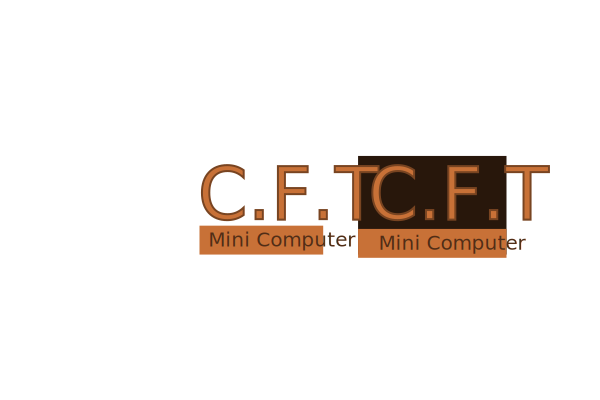
\includegraphics{figs/cft-logo-v1.pdf}\vspace{2em}\\
%% {\LARGE\bfseries CFT Minicomputer Programming Guide}
%% \vspace{10pt}

%% {\Large Alexios Chouchoulas}\\\vspace{5pt}
%% {\large \hyperemail{alexios@bedroomlan.org}}

%% \vspace{20pt}

%% %  \begin{abstract}
%%     \small
    
%%   This document discusses the architecture of the CFT computer from a
%%   programmer's perspective. The CFT is a solid-state, 16-bit,
%%   microcoded architecture reminiscent, among others, of the DEC
%%   PDP-8. The computer incorporates a 16-bit word width with separate
%%   memory and input/output addressing spaces and a minimal, orthogonal
%%   instruction set that is still particularly versatile. The design
%%   includes separate internal (processor) and external (peripheral)
%%   buses and is extensible both via processor extensions and
%%   peripherals.

%%   A brief explanation of the architecture is provided, along with a
%%   discussion of its programming model, instruction set, and
%%   limitations. Short examples of CFT Assembly code are provided, along
%%   with a complete opcode table with semantics and timing information.
    
%  \end{abstract}
  
%  \chapter{History of Changes}

  {\bfseries 2011-10-10} First draft compiled from notes, hardware description
  and schematics.

  {\bfseries 2011-10-18} Fixed hexadecimal opcode of macro \instr{ING} in the
  instruction table. Corrected minor semantic and typesetting errors.
  
  {\bfseries 2011-11-06} Added datapath diagram and description. Minor typo
  corrections.

  {\bfseries 2011-11-15} Added \instr{SEL} macro.

  {\bfseries 2011-11-17} Overflow detection and new instructions. Covered
  changes from Microcode Version 3 (\instr{OP1} and \instr{OP2} changes),
  register descriptions, new instructions.

  {\bfseries 2011-11-23} Accumulator acronym is now \A. Memory Address
  Register is now the Address Register (\AR). Various minor
  nomenclature changes and typographical errata.

  {\bfseries 2012-01-23} The {\sffamily R} instuction field is now reversed
  (microcode version 4).

  {\bfseries 2012-05-12} Further editing to account for microcode version 4,
  reworked figures.

%] % End of \twocolumn



%% \tikzset{boxes/.style={line width=2pt}}
%% \begin{figure*}[t!]
%%   \centering
%%   \begin{tikzpicture}[boxes]
%%     \begin{scope}[yshift=0cm]
%%       \draw[boxes, fill=red!30](0,0) rectangle (8,1);
%%       \draw (4,0.5) node {Microcode};
%%     \end{scope}

%%     \begin{scope}[yshift=1cm]
%%       \draw[boxes, fill=orange!30](0,0) rectangle (8,1);
%%       \draw (4,0.5) node {Instruction Set};
%%     \end{scope}

%%     \begin{scope}[yshift=2cm]
%%       \draw[boxes, fill=orange!30](0,0) rectangle (8,1);
%%       \draw (4,0.5) node {Instruction Macros and Extensions};
%%     \end{scope}

%%     \begin{scope}[yshift=3cm]
%%       \draw[boxes, fill=yellow!30](0,0) rectangle (8,1);
%%       \draw (4,0.5) node {Assembler Macros};
%%     \end{scope}

%%     \begin{scope}[yshift=4cm]
%%       \draw[boxes, fill=yellow!30](0,0) rectangle (8,1);
%%       \draw (4,0.5) node {Assembly Sub-programs};
%%     \end{scope}

%%     \begin{scope}[yshift=5cm]
%%       \draw[boxes, fill=green!30](0,0) rectangle (8,1);
%%       \draw (4,0.5) node {Forth Code Words};
%%     \end{scope}

%%     \begin{scope}[yshift=6cm]
%%       \draw[boxes, fill=cyan!30](0,0) rectangle (8,1);
%%       \draw (4,0.5) node {Native Forth Words};
%%     \end{scope}

%%     %% \begin{scope}[yshift=7cm]
%%     %%   \draw[boxes, fill=blue!30](0,0) rectangle (8,1);
%%     %%   \draw (4,0.5) node {Forth Applications};
%%     %% \end{scope}

%%     %% \begin{scope}[yshift=8cm]
%%     %%   \draw[boxes, fill=magenta!30](0,0) rectangle (8,1);
%%     %%   \draw (4,0.5) node {Higher Levels...};
%%     %% \end{scope}

%%   \end{tikzpicture}

%%   \caption{\label{fig-progmodel}Various levels of the CFT Programming Model.}

%% \end{figure*}



\section{Introduction}

  This document discusses the architecture of the CFT computer from a
  programmer's perspective. The CFT is a solid-state, 16-bit
  architecture reminiscent, among others, of the DEC
  PDP-8.\footnote{Newer versions of this document and additional
    documentation and downloads may be found at the following URL:\\
    \link{www.bedroomlan.org/hardware/cft}.}

  The computer incorporates a 16-bit word, 65,536 words of addressable
  main memory and 65,536 words of input/output (I/O) space.

  Instructions are 16-bits. There are ten \glspl{register} (five are 16-bits
  wide, the remaining five are single-bit flags) and a simple, nearly
  orthogonal instruction set. The computer is able to initialise itself without
  operator intervention using read-only ROM and a hardwired, turn-key bootstrap
  address. Communication to the outside world is attained using an interrupt
  facility, as part of a single expansion bus that connects to both main memory
  and peripherals. An autoindexing feature allows for very tightly coded
  looping structures.

  The design is microcoded for ease of upgrading.

\section{Architecture}

The CFT is a \gls{von Neumann architecture} \gls{stored program computer}. Data
is primarily manipulated in memory, using the system's single general-purpose
internal \gls{register} as an intermediate. The design is such that up to 1,024
general purpose memory-based registers may be accessed at any time. The
computer is completely solid-state, implemented using modern 74xxx integrated
circuits and some LSI memory.

The datapath of the CFT computer is shown in~\fcf{fig-datapath}. For
simplicity, it is built around a single bus, the \IBUS. All major
registers are connected to this bus.

The computer is microcoded. This simplifies upgrading and patching the
architecture to provide new features. Microcode consists of a number
of microprograms, each handling one CFT major state or
instruction. Each microprogram consists of up to 16 24-bit
microinstructions which operate directly the various physical units in
the computer and control the connection of registers and units to the
\IBUS.

The entire architecture is built around a 16-bit word. All data and
instructions is stored in 16-bit quantities, and all registers except
two are 16 bits wide. This allows programs and data to share the same
16-bit memory, and also makes programming significantly easier. A
rational, orthogonal instruction set with 16 main instructions and a
number of sub-instructions allows for ease of programming, yet
significant versatility.

The computer has separate address spaces for memory and input/output
devices, allowing the two to be kept separate. Through microcode
alterations additional wait states may be introduced for I/O, while
leaving memory accesses fast. This also allows processor extensions to
be built in I/O space, such as multiplication and division units,
novel instructions, et cetera.

\begin{figure*}
\includegraphics[width=\textwidth]{figs/datapath2.pdf}\vspace{2em}\\
\caption[Datapath]{\label{fig-datapath} The CFT datapath is organised around a
  single internal bus, the \IBUS. The {\em \gls{Accumulator}\/} (\A, bottom
  left) is the sole general-purpose internal register of the machine
  and is operated on by most instructions. A {\em Flag Unit\/} decodes
  the value of \A{} and accepts input from the \ALU{} to provide the
  basis for flow control. The \ALU{} performs all arithmetic and logic
  operations except register increments which are handled within the
  circuitry of those major registers that require it. The {\em Link\/}
  register (\Lreg) acts as a carry out register and extends \A{} by a
  single bit for certain operations. The {\em Control Unit\/} (centre)
  interprets microcode in response the the current instruction, which
  is stored in the {\em Instruction Register\/}. The {\em I Register}
  controls the reception of interrupts. The {\em Program Counter\/}
  (\PC) holds the location in memory of the next instruction to be
  fetched. The {\em Data Register\/} is an intermediate register used
  to implement indirect memory addressing. The {\em Memory Address
    Register\/} buffers addresses and directly drives the external
  address bus. The {\em Data Bus Transceiver\/} is a simple
  transceiver unit. When necessary, it connects the \IBUS{} to the
  external data bus to facilitate memory and I/O access. Finally, the
  {\em Constant Source\/} outputs to the \IBUS{} various constant
  values needed for resetting, address vectors, and other internal
  tasks.  }
\end{figure*}

\subsection{Word Size}

The word size is 16 bits. There are no facilities for accessing
quantities smaller than one word, and no single-instruction facilities
for accessing quantities longer than one word.

In this context, one kiloWord (kWord) is $2^{10}$ or 1,024 Words.

\subsection{Data Types}

CFT defines a single data type: a 16-bit unsigned integer,
i.e. integers in the range 0–65,535. There are no instructions
explicitly intended to handle signed numbers, but two's complement
operations may still be performed and the hardware has been designed
to make this easier.

\subsection{Addressing}

The CFT architecture can address up to 64~KWords of memory, plus up to
64~KWords of I/O space\footnote{Although, for practical reasons, 1
  KWord of I/O space is more readily available.}.

\subsubsection{Memory Space}
\label{sec:memory-space}

Main memory is split up into 64 {\em \gls{Page}s\/}, each 1 KWord in
size. Instructions usually reference memory addresses relative to the
page they are executing in.

The first page, Page Zero, is given special treatment by the
instruction set. If bit 10 (starting at zero) of an instruction is
clear, addresses in Page Zero may be accessed. This is the fastest and
most convenient way of accessing memory beyond the current page. As
such, Page Zero is always used for system variables, constants and
other data that must be globally accessible.

The 128 words in Zero Page addresses \hex{0080}–\hex{00FF} (inclusive)
are so-called Autoindex \glspl{register}. Using the Autoindex addressing
mode, each time one of these addresses is referenced, it is
automatically incremented by one. This allows loops to be coded very
tightly, with index register increments happening at the microcode
level.

\begin{figure}[bt]
  \centering
  \zebrahdr
  \begin{tabular}{cl}
    \hex{0000} & \asm{SUBRET} — return address for last \instr{JSR}.\\
    \hex{0001} & \asm{TRAPRET} — return address for last \instr{TRAP}\\
    \hex{0002} & \asm{ISRRET} — return address for last ISR.\\
    \hex{0080} & \asm{IR0} — first autoindex register.\\
    \hex{00FF} & \asm{IR7F} — last (128th) autoindex register.\\
    $\vdots$ & $\vdots$ \\
    \hex{03FF} & Last word of Page Zero.\\
    \hex{1000} & First word of Page 1.\\
    $\vdots$ & $\vdots$ \\
    \hex{8000} & First word of Page 32.\\
    $\vdots$ & $\vdots$ \\
    \hex{FC00} & First word of Page 63.\\
    \hex{FFF0} & Boot/reset address.\\
    \hex{FFF8} & Interrupt service routine.\\
    \hex{FFFF} & Highest memory address.\\
  \end{tabular}
  \caption{\label{fig-mm}Memory map of the CFT CPU's memory space.}
\end{figure}

\subsubsection{I/O Space}

Although there are 64 KWords of I/O space, this is limited by practical
limitations: Only the first 1,024 I/O addresses may be accessed from anywhere
in memory space (using the R field). Due to page-relative addressing, accessing
the rest of the I/O space is mostly convenient via indirect addressing. For
speed and ease of use, most I/O devices will thus occupy the first KWord of
address space. Page-relative addressing is discussed in detail in
\cf{sec-pagerel}.

\subsection{Registers}
\label{sec:registers}

\begin{figure}[tb]
  \centering
  % -*- latex -*-
\documentclass[class=memoir]{standalone}
% -*- latex -*-
\usepackage{pgf}
\usepackage{tikz}
%\usetikzlibrary{arrows,positioning,automata,shadows,fit,shapes,counters}
\usetikzlibrary{arrows,positioning,automata,shadows,fit,shapes,patterns}
%\usetikzlibrary{external}
%\tikzexternalize[prefix=tikz/]
%\tikzset{external/system call={xelatex \tikzexternalcheckshellescape -halt-on-error -interaction=batchmode -jobname "\image" "\texsource"}}
\usepackage{standalone}

\usepackage{layout}

%\usepackage[tocindentauto]{tocstyle}

%\usepackage[cam,a4,center]{crop}

\hypersetup{
    pdftitle={CFT Minicomputer Programming Guide},
    pdfauthor={Alexios Chouchoulas},
    pdfkeywords={},
    bookmarksnumbered,
    pagebackref=true,
    breaklinks=true,
%    pdfview=FitH,       % Or try pdfstartview={FitV}, This lead to uncorrect bookmarks
    urlcolor=darkblue,
    colorlinks=true,
    citecolor=cftoutline,          %citeref's color
    linkcolor=cftoutline,
        }

\makeindex
\makeglossaries
% -*- latex -*-

\renewcommand\glspostdescription{}

\newcommand\newglossaryabbr[3]{%
  \newglossaryentry{abbr#1}{name=\glslink{#1}{#2}, text={#2}, description={#3}}
  \newacronym[description={\glslink{abbr#1}{#2}}]{#1}{#1}{#2}
}

\newglossaryentry{IBUS}{name=IBUS,
  description={
  Internal Bus: the single, internal 16-bit bus of the CFT processor.
  }}
  
\newglossaryentry{Data Bus}{name=Data Bus, description={ A
    16-bit bus used to move data between the processor and
    peripherals.  }}
  
\newglossaryentry{Address Bus}{name=Address Bus, description={A
    16-bit bus used to select a peripheral nor memory location to
    access.}}
  
\newglossaryentry{Video Display Unit}{name=Video Display Unit,
  description={ Video Display Unit (VDU): a device that drives a
    display monitor to show character or graphics data on a
    screen. Often also contains one or more input devices (keyboard,
    mouse).}}
  
\newglossaryentry{von Neumann architecture}{name=Von Neumann architecture,
  description={ Named after the work of
    John von Neumann, the von Neumann architecture is a ‘modern’
    computer architecture that includes a register file, arithmetic
    and logic units, memory and input/output, and uses the same
    storage for programs and data.}}

\newglossaryentry{stored program computer}{name=Stored program computer,
  description={ A type of computer that
    uses the same storage for programs and data. All modern computers
    are stored program computers, allowing self-modification of their
    programs. Early designs and many modern microcontrollers stored
    programs and data in separate media, and did not or could not
    treat programs as data.}}

\newglossaryabbr{ALU}{Arithmetic/Logic Unit}{Describe this!}
\newglossaryabbr{ISR}{Interrupt Service Routine}{Describe this!}
\newglossaryentry{UART}{name=UART, description={
    Short for Universal Asynchronous Receiver/Transmitter. UARTs are
    devices that handle asynchronous serial communications such as RS-232, RS-485 or USB.
    }
}
%% \newglossaryentry{alu}{name=\glslink{ALU}{Arithmetic/Logic Unit}, text=Arithmetic/Logic Unit,
%%   description={TODO}}
%% \newacronym[description={\glslink{alu}{Arithmetic/Logic Unit}}]{ALU}{ALU}{Arithmetic/Logic Unit}

\newacronym{SBU}{SBU}{Skip/Branch Unit}

\newacronym{AGL}{AGL}{Address Generation Logic}

\newglossaryentry{DEB}{name=DEB, description={
    Designation of the CFT Debugging/Testing board, a peripheral that
    allows remote control and testing of the computer and its
    peripherals in the style of a virtual front panel. The DEB board
    is discussed in~\ccf{chap:deb}.
}}

\newglossaryentry{VDU}{name=VDU, description={ Video Display
    Unit. Designation of the CFT graphic card and keyboard
    controller. The VDU board is discussed in~\ccf{chap:vdu}.  }}

\newglossaryentry{MSB}{name=MSB, description={
    Most Significant Bits. Usually used to refer to the upper eight bits of a CFT word.
}}
\newglossaryentry{LSB}{name=LSB, description={
    Least Significant Bits. Usually used to refer to the lower eight bits of a CFT word.
}}

\newglossaryentry{NYBBLE}{name=Nybble, description={Sometimes
    nibble. A four-bit quantity, represented as a single hexadecimal
    digit.
}}

% \newacronym{MCU}{MCU}{Micro-Controller Unit}

\newglossaryabbr{MCU}{Micro-Controller Unit}{A single-chip device
  containing a simple microprocessor, general purpose input/output,
  serial input/output, timers, and other useful devices.}

\newacronym{USB}{USB}{Universal Serial Bus}

\newacronym{GPIO}{GPIO}{General-Purpose Input/Output}

\newglossaryentry{Verilog}{name=Verilog,
  description={
    One of the two major hardware
    description languages, the other being VHDL. In the CFT project,
    Verilog is used to perform 74xxx chip-level simulation and
    verification of the CFT processor.
}}

\newglossaryentry{I2C}{name=I²C, description={A two-wire, open-drain
    bus, often used for communication between \gls{MCU}s and
    peripheral chips, including EEPROMs and sensors. For more
    information, please consult
    \url{http://en.wikipedia.org/wiki/I2C}.}}

\newglossaryentry{data stack}{name=Data Stack,
  description=To Do}

\newglossaryentry{postfix}{name=postfix,
  description=To Do}

\newglossaryentry{stack effect comment}{name=stack effect comment,
  description=To Do}

\newglossaryentry{Wait State}{name=Wait State, 
  description={An additional state added to the processor state machine
  to accommodate slow devices. External devices signal their need for a
  wait state to the processor using an appropriate procotol. The
  processor then enters the Wait State and does not leave until the
  device is ready. The processor performs no action during this time,
  hence the name.}}


\newglossaryentry{Twos Complement}{name=Two's Complement,
  description={Currently the most popular means of representing signed
    integers in binary. For a bit width $n$, non-negative numbers $0 \leq
    x < 2^{n-1}$ are represented as unsigned $n$-bit binary
    integers. Negative numbers $-2^{n-1} \leq x < 0$ are represented in
    the form $2^n - x$, with the most significant bit set. On the CFT,
    with $n=16$, this provides a signed range of $[-32,768,
      32,767]$. Two's complement has many useful mathematical
    properties: only one representation of zero, the most significant
    bit also acts as a sign bit, and both addition and subtraction can
    be performed by the same circuitry. For a full discussion, please refer
    to \url{http://en.wikipedia.org/wiki/Two's\_complement}.  }}

\newglossaryentry{Assembly}{name=Assembly, description={A symbolic form of
    \gls{machine code}, meant to be used by humans. Some architectures,
    including the CFT, have simple machine code that can be learned in minutes,
    but the human brain deals better with symbols. Assembly languages also
    provide productivity enhancing features like comments, labels, macros,
    simple arithmetic for literals, and other such facilities. The CFT
    Assembler provides all of these facilities.  }}

\newglossaryentry{DIP}{name=DIP, description={Dual In-line Package, the
    most common integrated circuit package until the introduction of
    Surface Mount Technology: DIP chips have two rows of pins, with pins
    set at distances of 2.54~mm (0.1~inch).
}}

\newglossaryentry{PLCC}{name=PLCC, description={Plastic Leaded Chip
    Carrier, a square surface mount chip packaging easily adapted to
    2.54mm grids by means of suitable IC sockets. The CFT uses
    numerous PLCC chips to save board space and because they offer
    more choice of chips, and thus better value for money. All CFT
    PLCC packages are either Flash devices or UARTs.}}

\newglossaryentry{MEM}{name=MEM, description={ Designation of the
    memory board, which, depending on construction details provides up
    to 512 or 1,024 kWords of RAM and/or ROM. The MEM board is
    discussed in~\ccf{chap:mem}.
}}

\newglossaryentry{MBU}{name=MBU, description={Designation of the
    Memory Banking Unit. This was originally slated to be a separate
    peripheral, but has become so important to the project that it is
    now considered to be part of the processor, and constructed as
    such. The MBU breaks memory space in logical and physical
    addresses, and allows the processor's limited 64 kWord address
    space to be expanded to a 21 bit, 2,048 kWord address space using
    memory banking techniques. More details may be found in
    \ccf{chap:mbu}.  }}

\newglossaryentry{Interrupt Service Routine}{name=Interrupt Service Routine (ISR),
  description={TO DO}}

\newglossaryentry{Page}{name=Page, description={The CFT instruction set allows
    for a 10-bit operand, which allows instructions to address up to
    $2^{10}=1024$ locations. This 1,024-word range is known as a page. The CFT
    address space contains 64 such 1 kWord pages. \gls{Page Zero} at addresses
    \hex{0000}–\hex{03FF} has special significance in the programming model, as
    discussed in~\cf{sec:memory-space}.
 }}

\newglossaryentry{Page Zero}{name=Page Zero, description={Page Zero occupies
    the first 1,024 addresses (\hex{0000}–\hex{03FFF}) of the memory address
    space. It is used to simulate 1,024 registers, global variables or
    constants accessible from anywhere in memory. Addresses
    \hex{0080}–\hex{00FF} are autoindex locations: they increment when accessed
    in \gls{Indirect Mode}.}}

\newglossaryentry{Addressing Mode}{name=Addressing Mode, description={An
    addressing mode is the method in which an instruction operand is
    interpreted. The CFT can treat operands as literal values (\gls{Literal
      Mode}), addresses of data (\gls{Direct Mode}), or addresses of addresses
    of data (\gls{Indirect Mode}), similar to pointersin high-level languages
    such as C and Pascal. Addressing modes are discussed
    in~\cf{sec:addressing-modes}}.}

\newglossaryentry{Indirect Mode}{name=Indirect Mode, description={An addressing
    mode where an instruction operand identifies the memory location which
    contains the address of the data to access. Compare \gls{Direct
      Mode}. Addressing modes are discussed in~\cf{sec:addressing-modes}.}}

\newglossaryentry{Direct Mode}{name=Direct Mode, description={An addressing
    mode where an instruction operand identifies the memory location of the
    data to access. Compare \gls{Indirect Mode}. Addressing modes are discussed
    in~\cf{sec:addressing-modes}.}}

\newglossaryentry{Literal Mode}{name=Literal Mode, description={An addressing
    mode where an instruction operand identifies the memory location of the
    data to access. Compare \gls{Indirect Mode}. Addressing modes are discussed
    in~\cf{sec:addressing-modes}.}}

\newglossaryentry{register}{name=Register, description={ A data storage device
    inside a processor. Registers are usually faster than memory, and so are
    used to store intermediate results. In many architectures, notably
    \glspl{ABA}, the only way for the processor to
    manipulate data is to transfer it to a register, operate on the register,
    then transfer it back to its intended location. CFT registers are discussed
    in~\cf{sec:registers}.}}

\newglossaryentry{Accumulator}{name=Accumulator, description={The main
    \gls{register} in an \gls{ABA}. Data must be transferred to the Accumulator
    before it can be operated on by the processor. In the CFT, the Accumulator
    is the only such general purpose register available. The term comes from
    the days of tabulating machines, which used accumulators to accumulate
    (sum) numbers. The Accumulator is designated ‘\AC’ on the CFT. Its hardware
    design is discussed in~\cf{sec:major-registers} and its operation from a
    programmer's point of view is discussed in~\cf{sec:accumulator}.}}

\newglossaryabbr{ABA}{Accumulator-Based Architecture}{A processor architecture
  built around a single (or in some cases, a few) accumulators. Most early
  computers followed this design because of its simplicity, and the CFT does
  too. Having a single register draastically simplifies the instruction format,
  too: from a two-operand instruction format (source, destination), we move to
  a single operand (source or destination). The other operand is always the
  accumulator.  }

\newglossaryentry{nybble}{name=Nybble, description={(sometimes nibble)
    A 4-bit quantity, corresponding to one hexadecimal digit, half a
    byte, or one quarter of a CFT \gls{Word}.}}

\newglossaryentry{Word}{name=Word, description={One CFT Word is a
    16-bit quantity. CFT memory and I/O accesses transfer exactly one
    word each. CFT instructions are also one Word wide. This is not to
    be confused with the Forth concept of a \gls{word} (an identifier).}}

\newglossaryentry{word}{name=Word, description={A Forth word is any
    sequence of non-whitespace characters that is not a number. This
    is not to be confused with the more common concept of the
    \gls{Word} as a numeric datatype.}}

\newglossaryentry{machine code}{name=Machine code, description={Machine code is
    the native language of every processor, where machine instructions and data
    are represented in binary. Machine code is easy for the computer to
    process, but humans find it useful to apply abstraction layers to it: data
    are represented in other bases (octal, decimal and hexadecimal being the
    most common), and symbolic instruction names (rather than binary
    instruction numbers) are used. This set of abstractions is \gls{Assembly}
    language.}}

\newglossaryentry{disk label}{name=Disk Label, description={ A disk label
    stores information about a storage device (not always a disk), including a
    magic number to help detect the block, some optional boot code, and
    definitions for one to sixteen \glspl{disk slice} (partitions). The disk
    label always resides in the first block of a device. The best-known disk
    label format is the MS-DOS Master Boot Record, MBR. The CFT's disk label is
    discussed in~\cf{sec:disk-label}.}}

\newglossaryentry{disk slice}{name=Disk Slice, description={Part of a disk intended to
    hold a \gls{filesystem} or other data. Disks are sliced to make them easier
    to manage, so different operating systems can be used, to control the size
    of stored data, and to avoid corruption in one filesystem destroying all
    data. In the MS-DOS world, slices are known as ‘partitions’, and the
    \gls{disk label} is known as a ‘partition table’ or ‘Master Boot Record’
    depending whether it resides on a data disk or bootable disk. The CFT's
    slice scheme is discussed in~\cf{sec:disk-slices}}.}

\newglossaryentry{filesystem}{name=Filesystem, description={ A large data
    structure used to view a storage medium as a hierarchical collection of
    data objects called files. The filesystem abstracts the natural
    array-of-blocks structure of the storage medium, and provides the user with
    an interface for creating, reading and otherwise operating on files by
    their name, location and other attributes. Files can be larger than the
    natural block size, and this is again handled transparently by the
    filesystem code. The CFT's filesystem is described in~\cf{sec:fs}}}

\newglossaryabbr{VD}{Volume Directory}{A data structure
  describing a CFT \gls{filesystem}. Comparable to a Unix filesystem
  superblock. The VDD is the exact same data structure as a
  \gls{DD}. The difference is in the magic number and the contents of
  the first directory slot (the header), which contains a volume
  header structure.}

\newglossaryabbr{DD}{Directory Descriptor}{A data structure describing
  a directory in a CFT \gls{filesystem}.}

\newglossaryentry{block pointer}{name=Block Pointer, description={A
    32-bit value (\gls{MSB} first) denoting the number of a filesystem
    block. A filesystem's first block is block \hex{00000000}.}}

\newglossaryabbr{DH}{Directory Header}{A data structure describing a
  CFT directory. This is the first entry of a \gls{DD}.}

\newglossaryabbr{OOP}{Object Oriented Programming}{A programming
  paradigm where data and code are bundled together in data structures
  called objects. Programs are built based on the interactions and
  interrelations of these objects.}

\newglossaryentry{descriptor}{name=Descriptor, description={In the CFT Filesystem, a data structure
    that holds metadata on an object in the CFT filesystem. Descriptors share
    some common metadata (e.g. filenames, flags, creation time and date). They
    are located inside container objects (volumes and directories). Containers
    and descriptors are discussed in~\cfp{sec:fs-containers}.}}

\newglossaryentry{volume}{name=Volume, description={A \gls{disk slice} which
    has been structured according to the CFT Filesystem. In \gls{OOP} terms, a
    volume is the object (instance) and the CFT Filesystem is the class.}}

\newglossaryentry{container}{name=Container, description={In the CFT
    Filesystem, a data structure that contains other filesystem objects. Entire
    filesystem \glspl{volume} are containers, and so are directories. Each
    container owns a maximum number of \glspl{descriptor}, identifying the
    contained objects. Once this limit is reached, continuation blocks are
    allocated for the container. These continuation blocks form a doubly linked
    list. Containers are discussed in~\fcf{sec:fs-containers}.}}

\newglossaryabbr{PEL}{Picture Element}{The smallest addressable
  picture element of a display mode. A PEL is usually a block of
  multiple pixels.}

\newglossaryabbr{MTBF}{Mean Time Between Failures}{The average life
  expectancy of a device.}

\newglossaryentry{codepoint}{name=Codepoint, description={A number
    identifying a character within a character set. For example, in
    the ASCII set, codepoint 65 is the character ‘A’.}}

\newglossaryabbr{SDRAM}{Synchronous Dynamic Random Access Memory}{A
  type of modern dynamic RAM that operates using a clock, not
  asynchronously like original DRAMs. The memory contains a command
  pipeline, because data appears on the bus two to three clock ticks
  after a read is signalled. Multiple reads are pipelined, making the
  memory very fast for many use patterns.}

\newglossaryabbr{SRAM}{Static Random Access Memory}{A type of
  relatively low-density memory that trades off capacity and price for
  speed and interface simplicity. SRAMs do not need to be refreshed
  and are faster than similar dynamic RAMs.}

\newglossaryentry{extended instruction}{name=Instruction!Extended,
  description={An address in I/O space that provides side effects
    useful enough to be seen as extending the processor's instruction
    set. They are usually aliases of single \asm{IN}, \asm{OUT} or
    \asm{IOT} instructions.}}

\newglossaryabbr{SR}{Switch Register}{A 16-bit read-only register that
  provides the value of the 16 data entry switches on the front
  panel.}

\newglossaryabbr{DSR}{DIP Switch Register}{A 12 to 16-bit read-only
  register driven by a bank of DIP switches on the Front Panel
  Controller board. The DSR can be used to set non-volatile prefrences
  for the computer's early boot.}

\newglossaryabbr{MFD}{Multi-Function Display}{A bank of 16 lights on
  the front panel which can display a user-selectable register. The
  user can elect to show the value of the Data Register, Output
  Register, or the 15-bit microcode store address. A switch on the
  front panel is used to do this.}


\usepackage{listings}
\lstset{%
  xleftmargin=35pt,
  xrightmargin=5pt,
  basicstyle={\ttfamily},
  backgroundcolor=\color{cfthl!25},
  rulecolor=\color{cfthl!25},
  framesep=5pt,
  rulesep=5pt,
  frame=tlrb,
  framexleftmargin=10pt,
  flexiblecolumns=true,
  keepspaces=true,
  numbers=left,
  numbersep=5pt,
  numberstyle={\scriptsize\sffamily\color{cftlight}}
}




%%%%%%%%%%%%%%%%%%%%%%%%%%%%%%%%%%%%%%%%%%%%%%%%%%%%%%%%%%%%%%%%%%%%%%%%%%%%%%%
%%
%% LISTS OF THINGS
%%
%%%%%%%%%%%%%%%%%%%%%%%%%%%%%%%%%%%%%%%%%%%%%%%%%%%%%%%%%%%%%%%%%%%%%%%%%%%%%%%

%% %%%\addtolength\cftfignumwidth{1.5em}
\makeatletter
%% \addtolength{\cftchapternumwidth}{0.5em}
%% \addtolength{\cftsectionnumwidth}{0.5em}
%% \addtolength{\cftsubsectionnumwidth}{0.5em}
%% \addtolength{\cftfigurenumwidth}{0.5em}
%% \addtolength{\cfttablenumwidth}{0.5em}
\renewcommand*\l@section{\@dottedtocline{1}{1.5em}{2.3em}}
\renewcommand*\l@subsection{\@dottedtocline{2}{3.8em}{3.2em}}
\renewcommand*\l@subsubsection{\@dottedtocline{3}{7.0em}{4.1em}}
\renewcommand*\l@paragraph{\@dottedtocline{4}{10em}{5em}}
\renewcommand*\l@subparagraph{\@dottedtocline{5}{12em}{6em}}
\setcounter{maxsecnumdepth}{3}

%\addtolength{\cftschematicsnumwidth}{1em}
\renewcommand{\@pnumwidth}{3em}
\renewcommand{\@tocrmarg}{4em}
\makeatother

%\newcommand\listalgname{List of Algorithms} 
%\newlistof{alg}{algorithm}

%
% Schematics
%

\newcommand\listschematicname{List of Schematics} 
\newlistof{listofschematic}{los}{\listschematicname}
\newcounter{schematic}
\newcommand{\schematic}[1]{%
  \refstepcounter{schematic}%
  \par\noindent\textbf{Schematic \theschematic. #1}
  \addcontentsline{los}{section}{\protect\numberline{\theschematic}#1}\par%
}
\newcommand\listofschematics\listofschematic

%
% I/O Ports
%

\newcommand\listioportname{List of Input/Output Ports} 
\newlistof{listofioport}{loioport}{\listioportname}
%% \newcommand{\registerioport}[1]{%
%%   \refstepcounter{ioport}%
%%   \addcontentsline{loioport}{section}{\protect\numberline{\ }%
%% }
\newcommand\listofioports\listofioport



\newcommand\caution[1]{\textcolor{caution}{\textbf{#1}}}
%\newcommand\todo[1]{\textcolor{caution}{\bf{TODO: #1}}}

%
% Tasks
%

\newcommand\listtasksname{List of Incomplete Tasks} 
\newlistof{listoftask}{lotasks}{\listtasksname}
\newcounter{task}
\newcommand{\todo}[1]{%
  \refstepcounter{task}%
  {\textcolor{caution}{\textbf{TODO: #1}}}
  \addcontentsline{lotasks}{section}{\protect\numberline{\arabic{task}}To Do: #1}\par%
}
\newcommand{\bug}[2]{%
  \refstepcounter{task}%
  {\textcolor{caution}{\textbf{BUG: #1 #2}}}
  \addcontentsline{lotasks}{section}{\protect\numberline{\arabic{task}}Bug: #1}\par%
}
\newcommand\listoftasks\listoftask

%
% Data structures
%

\newcommand\listdatastructurename{List of Data Structures} 
\newlistof{listofdatastructure}{lods}{\listdatastructurename}
\newcounter{datastructure}
%\newcommand{\datastructure}[1]{%
%  \refstepcounter{datastructure}%
%  \par\noindent\textbf{Data Structure \thedatastructure. #1}
%  \addcontentsline{lods}{section}{\protect\numberline{\thedatastructure}#1}\par%
%}
\newcommand\listofdatastructures\listofdatastructure



%%%%%%%%%%%%%%%%%%%%%%%%%%%%%%%%%%%%%%%%%%%%%%%%%%%%%%%%%%%%%%%%%%%%%%%%%%%%%%%
%%
%% SECTION STYLING
%%
%%%%%%%%%%%%%%%%%%%%%%%%%%%%%%%%%%%%%%%%%%%%%%%%%%%%%%%%%%%%%%%%%%%%%%%%%%%%%%%



%% \usepackage{kpfonts}
\usepackage[explicit]{titlesec}

\counterwithin*{chapter}{part}
\counterwithin*{figure}{chapter}
\counterwithin*{schematic}{chapter}
\counterwithin*{datastructure}{chapter}
\counterwithin*{table}{chapter}

%%%%%%%%%%%%%%%%%%%%%%%%%%%%%%%%%%%%%%%%%%%%%%%%%%%%%%%%%%%%%%%%%%%%%%%%%%%%%%%

\renewcommand\thepart{\Alph{part}}
\cftpagenumbersoff{part}
%\newcommand*\partlabel{}

\makeatletter
\patchcmd{\l@part}{\hss#2}{}{}{}
\makeatother


\renewcommand\partnamefont{\normalfont\sffamily\Huge\scshape}
\renewcommand\partnumfont{\bfseries}
\renewcommand\printparttitle[1]{
  \thispagestyle{empty}
    \begin{tikzpicture}[remember picture,overlay]
      \node[yshift=-\paperheight, draw opacity=0] at (current page.north west)
           {\begin{tikzpicture}[remember picture, overlay]
               \draw[fill=cftlight] (0,0) rectangle
               (\paperwidth,\paperheight);
               \draw[fill=cftoutline] (0,1cm) rectangle
               (\paperwidth,0);
               \node[anchor=east,yshift=0.5\paperheight,xshift=.87\paperwidth,rectangle]
                    {\scalebox{2}{\color{white}\printpartname~\printpartnum}};
                    \node[anchor=east,yshift=0.43\paperheight,xshift=.87\paperwidth,rectangle]
                         {\scalebox{1.5}{\color{white} #1}};
             \end{tikzpicture}
           };
    \end{tikzpicture}
}


\newcommand*\chapterlabel{}
\titleformat{\chapter}
  {\gdef\chapterlabel{}
   \normalfont\sffamily\Huge}
  {\gdef\chapterlabel{\thechapter\ }}{0pt}
  {%
    \setcounter{page}{1}
    \begin{tikzpicture}[remember picture,overlay]
    \node[yshift=-5cm, draw opacity=0] at (current page.north west)
      {\begin{tikzpicture}[remember picture, overlay]
        \draw[fill=cftlight] (0,0) rectangle
          (\paperwidth,5cm);
        \draw[fill=cftoutline] (0,0.25cm) rectangle
          (\paperwidth,0);
        \node[anchor=east,yshift=2cm,xshift=.87\paperwidth,rectangle]
              {\color{white}\chapterlabel#1};
       \end{tikzpicture}
      };
   \end{tikzpicture}
  }
\titlespacing*{\chapter}{0pt}{50pt}{20pt}

\titleformat{\section}
            {\gdef\sectionlabel{}\normalfont\sffamily\Large}
            {\gdef\sectionlabel{\thesection\ }}{0pt}
            {\color{cftoutline}\thesection\quad #1\\
              \titlerule[2pt]
            }[{\vspace{-30pt}\color{cftoutline}\rule{\textwidth}{2pt}}]


\titleformat{\subsection}
  {\gdef\subsectionlabel{}
   \normalfont\sffamily\bfseries\large}
  {\gdef\subsectionlabel{\thesubsection\ }}{0pt}
  {\color{cftoutline}\thesubsection\quad #1}


\titleformat{\subsubsection}
  {\gdef\subsubsectionlabel{}
   \normalfont\sffamily\large}
  {\gdef\subsubsectionlabel{\thesubsubsection\ }}{0pt}
  {\color{cftoutline}#1}


%%%%%%%%%%%%%%%%%%%%%%%%%%%%%%%%%%%%%%%%%%%%%%%%%%%%%%%%%%%%%%%%%%%%%%%%%%%%%%%










%% \titleformat{\paragraph}
%%   {\gdef\chapterlabel{}
%%    \normalfont\bfseries}
%%   {\gdef\chapterlabel{\theparagraph\ }}{0pt}
%%   {\color{cftoutline}#1}



%\geometry{a4paper, hoffset=0in, voffset=-.25in, left=1.5cm, right=1.5cm,
%  top=2.5cm, bottom=2.5cm}
%\geometry{paperwidth=17.5cm, paperheight=23.1cm, hoffset=0in, voffset=-.25in, left=1in, right=1in,
%  top=1in, bottom=1in}
\geometry{a4paper, hoffset=0in, left=1.2in, right=1.2in,
  top=1.2in, bottom=1.2in, includefoot, footskip=40pt}
%\sloppy


% Fonts
%\defaultfontfeatures{Mapping=tex-text}
\setmainfont{Minion Pro}
\setsansfont{Myriad Pro}
\setmonofont[]{Inconsolata}


% Not really used here, but never mind.
\setlength\columnsep{7mm}


% Input our local macro definitions
% -*- latex -*-

\definecolor{caution}{RGB}{192,0,0}

\newcommand\textcond{\fontspec{Myriad Pro Condensed}}

% Primary index entries
\newcommand\pie[1]{\textbf{\hyperpage{#1}}}

% Use hyperlinking when rendering PDFs
\newcommand{\barecf}[1]{\hyperref[#1]{\ref*{#1}}}
\newcommand{\cf}[2][section]{\hyperref[#2]{%
        \ifthenelse{\equal{\pageref*{#2}}{\thepage}}%
        {#1 \ref*{#2}}%
        {#1 \ref*{#2} (p.~\pageref*{#2})}%
}}
\newcommand{\cfp}[2][section]{\hyperref[#2]{%
        \ifthenelse{\equal{\pageref*{#2}}{\thepage}}%
        {#1 \ref*{#2}}%
        {#1 \ref*{#2}, p.~\pageref*{#2}}%
}}
\newcommand{\fcf}[1]{\cf[figure]{#1}}
\newcommand{\fcfp}[1]{\cfp[figure]{#1}}
\newcommand{\tcf}[1]{\cf[table]{#1}}
\newcommand{\tcfp}[1]{\cfp[table]{#1}}
\newcommand{\ccf}[1]{\cf[chapter]{#1}}
\newcommand{\ccfp}[1]{\cfp[chapter]{#1}}
%
\newcommand{\npcf}[2][section]{\hyperref[#2]{#1 \ref*{#2}}}
\newcommand{\appcf}[1]{\cf[appendix]{#1}}
\newcommand{\ecf}[1]{\cf[equation]{#1}}
\newcommand{\algcf}[1]{\cf[algorithm]{#1}}
\newcommand{\npappcf}[1]{\npcf[appendix]{#1}}
\newcommand{\npccf}[1]{\npcf[chapter]{#1}}
\newcommand{\npfcf}[1]{\npcf[figure]{#1}}
\newcommand{\nptcf}[1]{\npcf[table]{#1}}
\newcommand{\npecf}[1]{\npcf[equation]{#1}}
\newcommand{\npalgcf}[1]{\npcf[algorithm]{#1}}

\newcommand\hyperemail[1]{\sffamily\href{mailto:#1}{#1}}
\newcommand\link[1]{\sffamily\href{http://#1}{#1}}
\newcommand\ahref[2]{\sffamily\href{#1}{#2}}

\newcommand\op[1]{{\ttfamily #1}}
\newcommand\fwni[1]{{\ttfamily{#1}}}
\newcommand\fw[1]{\fwni{#1}\index{#1@\protect\fwni{#1}}}
%                           \index{#1@\fwni{#1}|(pie}%

\newcommand\f[1]{{\texttt{#1}}}
\newcommand\hex[1]{\textsf{#1}}
\newcommand\bin[1]{\textsf{#1}}
\newcommand\bitmap[1]{\texttt{#1}}
\newcommand\bus[1]{{#1}}
\newcommand\unit[1]{{#1}}
\newcommand\IBUS{\bus{\gls{IBUS}\index{IBUS}}}
\newcommand\DBUS{\bus{\gls{Data Bus}\index{Data Bus}}}
\newcommand\ABUS{\bus{\gls{Address Bus}\index{Address Bus}}}
\newcommand\ALU{\unit{\gls{ALU}\index{ALU}}}
\newcommand\SBU{\unit{\gls{SBU}\index{SBU}}}
\newcommand\AGL{\unit{\gls{AGL}\index{AGL}}}
\newcommand\register[1]{\textsf{#1}\index{Registers!#1}}
\newcommand\A{\register{AC}}
\newcommand\AC{\A}
\newcommand\Areg{\A}
\newcommand\Lreg{\register{L}}
\newcommand\Ireg{\register{I}}
\newcommand\Zreg{\register{Z}}
\newcommand\Vreg{\register{V}}
\newcommand\Nreg{\register{N}}
\newcommand\AR{\register{AR}}
\newcommand\MAR{\AR}
\newcommand\DR{\register{DR}}
\newcommand\PC{\register{PC}}
\newcommand\IR{\register{IR}}

\newcommand{\asm}[1]{\texttt{#1}}
\newcommand{\instr}[1]{\asm{#1}}
\newcommand{\nsni}[1]{$\overline{\mbox{\textsf{{#1}}}}$}
\newcommand{\ns}[1]{\nsni{#1}\index{#1@{$\protect\overline{\protect\mbox{\textsf{#1}}}$}}}
\newcommand{\psni}[1]{\textsf{#1}}
\newcommand{\ps}[1]{\psni{#1}\index{#1@\psni{#1}}}
\newcommand{\lt}[1]{\textsf{#1}}
\newcommand{\sw}[1]{\textsf{#1\index{Switch, front panel!#1}}}
\newcommand{\HC}[1]{\chip{74HC{#1}}}
\newcommand{\HCT}[1]{\chip{74HCT{#1}}}
\newcommand{\chip}[1]{#1\index{#1}}

\newcommand{\schpt}[1]{#1\textsf{#1}}
\newcommand{\farnell}[1]{#1}

\newcommand\BUS[2]{\ps{#1}$_{\mbox{\scriptsize #2}}$}
\newcommand\nBUS[2]{\ns{#1}$_{\mbox{\scriptsize #2}}$}

\newcommand\UINSTR{\ns{uINSTR18}}
\newcommand\HALT{\ns{HALT}}
\newcommand\END{\ns{END}}
\newcommand\IRQ{\ns{IRQ}}
\newcommand\IRQS{\ns{IRQS}}
\newcommand\IRQn[1]{\nBUS{IRQ}{#1}}
\newcommand\RUNITn[1]{\BUS{RUNIT}{#1}}
\newcommand\WUNITn[1]{\BUS{WUNIT}{#1}}
\newcommand\TPA{\ps{TPA}}
\newcommand\TPC{\ps{TPC}}
\newcommand\WAC{\ns{WAC}}
\newcommand\WALU{\ns{WALU}}
\newcommand\WDR{\ns{WDR}}
\newcommand\WIR{\ns{WIR}}
\newcommand\WMAR{\ns{WMAR}}
\newcommand\WPC{\ns{WPC}}
\newcommand\SYSDEV{\ns{SYSDEV}}
\newcommand\IODEV[1]{\ns{IODEV{#1}XX}}
\newcommand\OPIFn[1]{\BUS{OPIF}{#1}}
\newcommand\OPIF{\ps{OPIF}}
\newcommand\GUARDPULSE{\ns{GUARD}}
\newcommand\GP{\GUARDPULSE}
\newcommand\CLOCK[1]{\BUS{CLK}{#1}}
\newcommand\RSTHOLD{\ns{RSTHOLD}}
\newcommand\BOE{\ns{BOE}}
\newcommand\UOE{\ns{UOE}}
\newcommand\SKIP{\ns{SKIP}}
\newcommand\AINDEX{\ps{AINDEX}}
\newcommand\CLL{\ns{CLL}}
\newcommand\CPL{\ns{CPL}}
\newcommand\CLI{\ns{CLI}}
\newcommand\STI{\ns{STI}}
\newcommand\IRn[1]{\BUS{IR}{#1}}
\newcommand\PCn[1]{\BUS{PC}{#1}}
\newcommand\IBUSn[1]{\BUS{IBUS}{#1}}
\newcommand\IRn[1]{\BUS{IR}{#1}}
\newcommand\ACn[1]{\BUS{AC}{#1}}
\newcommand\DBUSn[1]{\BUS{DBUS}{#1}}
\newcommand\ABUSn[1]{\BUS{AB}{#1}}
\newcommand\AEXTn[1]{\BUS{AEXT}{#1}}
\newcommand\ISROLL{\ps{ISROLL}}
\newcommand\RAC{\ns{RAC}}
\newcommand\RAGL{\ns{RAGL}}
\newcommand\RDR{\ns{RDR}}
\newcommand\RPC{\ns{RPC}}
\newcommand\INCPC{\ns{INCPC}}
\newcommand\STPAC{\ns{STPAC}}
\newcommand\STPDR{\ns{STPDR}}
\newcommand\INCAC{\STPAC}
\newcommand\INCDR{\STPDR}
\newcommand\DEC{\ns{DEC}}
\newcommand\MEM{\ns{MEM}}
\newcommand\IO{\ns{IO}}
\newcommand\R{\ns{R}}
\newcommand\WRITE{\ns{W}}
\newcommand\WEN{\ns{WEN}}
\newcommand\READ{\ns{R}}
\newcommand\FL{\ps{FL}}
\newcommand\FV{\ps{FV}}
\newcommand\FZERO{\ps{FZERO}}
\newcommand\FNEG{\ps{FNEG}}
\newcommand\RESET{\ns{RESET}}
\newcommand\abbr[1]{#1}
\newcommand\SKIPEXT{\ns{SKIPEXT}}
\newcommand\ENDEXT{\ns{ENDEXT}}
\newcommand\WS{\ns{WS}}
\newcommand\UPC{\ps{µPC}}
\newcommand\UCB{\ps{µCB}}

\newcommand\NB{\textbf{Nota Bene:\ }}

\newcommand\bit[1]{{\texttt{#1}}}

\newcommand\notes[1]{{\small\verbatiminput{#1}}}

\newcommand\field[1]{\textsf{#1}}
\newcommand\port[1]{\textsf{#1}}

\newcommand\cftin[1]{\textsf{#1}}
\newcommand\cftout[1]{\textsf{#1}}
\let\cftcode\cftout
\let\cftkbd\cftin

\newcommand\li[1]{\item{\bfseries #1}}

% Temporary question environment
\newcommand\question[2]{\textbf{#1} #2}


%%%%%%%%%%%%%%%%%%%%%%%%%%%%%%%%%%%%%%%%%%%%%%%%%%%%%%%%%%%%%%%%%%%%%%%%%%%%%%%
%
% THE I/O PORT AND EXTENDED COMMAND INDEX
%
%%%%%%%%%%%%%%%%%%%%%%%%%%%%%%%%%%%%%%%%%%%%%%%%%%%%%%%%%%%%%%%%%%%%%%%%%%%%%%%

%% \makeatletter
%% \newcommand\ioport@[4]{%
%%   \label{ioport:#1-#4}
%%   \vspace{0.5em}
%%   \noindent\hex{\bfseries{#2}} (\texttt{#1}): {\bfseries\asm{\bfseries{#3}}} — {#4}
%%   \vspace{0.5em}
%% }
%
%
% \ioport{port}{crwvehf}{regname}{descr}
%
%% \newcommand\ioport[4]{%
%%   \ioport@{#1}{#2}{#3}{#4}
%%   \addcontentsline{loioport}{section}{\hex{#2} (\texttt{#1}) \textbf{\asm{#3}} — soup}%
%% }

% \begin{ioport}{VDU}{1F0}{--wvehf}{MCR0}{Mode Control Register 0}
% ...
% \end{ioport}

\newenvironment{ioport}[5]{%
  \vspace{0.5em}
  \addcontentsline{loioport}{section}{\hex{#2} (\texttt{#3}) \textbf{\cftout{#1} \cftout{#4} — #5}}%
  \noindent\hex{\bfseries{#2}} (\texttt{#3}): {\bfseries\asm{\bfseries{#4}}} — {#5}%
  \noindent%
}{%
  \vspace{0.5em}
}

% \begin{extcmd}{PFP}{SR1}{4409}{009}{--wvehf}{Mode Control Register 0}
% ...
% \end{extcmd}
\newenvironment{extcmd}[7]{%
  \vspace{0.5em}
  \addcontentsline{loioport}{section}{\hex{#2} (\texttt{#4}) \textbf{\cftout{#1} \cftout{#2} — #6}}%
  \noindent\hex{\bfseries{#2}} \hex{#3} (I/O port \hex{#4} — \texttt{#5}): {\bfseries{#6}}%
  \noindent%
}{%
  \vspace{0.5em}
}

%\newcommand\extcmda[7]{%
%  \label{ioport:#5-#2}
%  \vspace{0.5em}
%  \noindent\hex{\bfseries{#2}} (\texttt{#1}): {\bfseries\asm{\bfseries{#3}}} — {#4}
%  \vspace{0.5em}
%  \ioport{#4}{#5}{#1}{#7}
%}
%\newcommand\extcmd[7]{% 
%  \extcmda{#1}{#2}{#3}{#4}{#5}{#6}{#7}
%  \addcontentsline{loioport}{section}{\hex{#5} (\texttt{#4}) \textbf{\asm{#1}} — {#6}}%
%  \addcontentsline{loioport}{section}{\protect\numberline{\ }%
%}
\makeatother


%%%%%%%%%%%%%%%%%%%%%%%%%%%%%%%%%%%%%%%%%%%%%%%%%%%%%%%%%%%%%%%%%%%%%%%%%%%%%%%
%
% CODE FOR DISPLAYING AND INDEXING SCHEMATICS
%
%%%%%%%%%%%%%%%%%%%%%%%%%%%%%%%%%%%%%%%%%%%%%%%%%%%%%%%%%%%%%%%%%%%%%%%%%%%%%%%


% \schematic{page number}{description}{label}
\def\schematicsFile{figs/schematics.pdf}
\newcommand\includesch[3]{%
  \stepcounter{subsection}%
  \phantomsection%
  \addcontentsline{toc}{subsection}{\protect\numberline{\thesubsection} #2}%
  \includeschns{#1}{#2}{#3}
}

\newcommand\includeschns[3]{%
  \label{#3}%
  \stepcounter{schematic}%
  \addcontentsline{los}{section}{\protect\numberline{\theschematic} #2}%
  \includepdf[
    pages={#1}
    ,landscape,
    ,fitpaper=true,
%    ,pagecommand={\thispagestyle{lscape}}  
    ,pagecommand={\thispagestyle{empty}}  
  ]{\schematicsFile}%
}


\newcommand\tU{$\uparrow$}
\newcommand\tD{$\downarrow$}

\newcommand\lstkbd[1]{\mathbf{\textbf{#1}}}
%\newcommand\lstfkbd[1]{\underline{\mathbf{\textbf{#1}}}}
\newcommand\lstfkbd[1]{\color{cftoutline}{\mathbf{\textbf{#1}}}}
\lstset{%
        keywordstyle=\fontspec{Inconsolata Bold},%
        keywordstyle=[2]\color{cftoutline}\fontspec{Inconsolata Bold},%
        keywordstyle=[3]\fontspec{Inconsolata Bold},%
        commentstyle=\color{cftlight}%
}
\lstdefinestyle{deb}{mathescape=true,numbers=none}
\lstdefinestyle{forthprogram}{}
\lstdefinelanguage{cftasm}{%
        mathescape=true,
        morekeywords={TRAP,IOT,LOAD,STORE,IN,OUT,JMP,JSR,ADD,AND,OR,%
                      XOR,OP1,OP2,ISZ,LIA,R,I,IFL,IFV,CLA,CLL,NOT,%
                      INC,CPL,RBL,RBR,RNL,RNR,NOP,SNA,SZA,SSL,SSV,SKIP,%
                      SNN,SNZ,SCL,SCV,CLI,SEI,SEL,NEG,ING,LI,SPA,SNP,RET,%
                      RTT,RTI,SBL,SBR},%
        morekeywords=[2]{.equ,.reg,.include,.word,.fill,%
                      .str,.data,.strp,.strn,.page,.macro,.end},%
        alsoletter=.,%
        sensitive=false,%
        morecomment=[l]{/},%
        morecomment=[l]{;},%
}

\lstdefinestyle{longmcasm}{%
        language=mcasm,
        xleftmargin=25pt,
        xrightmargin=5pt,
        framexleftmargin=20pt,
        basicstyle={\footnotesize\ttfamily},
}
\lstdefinelanguage{mcasm}{%
        mathescape=false,
        morekeywords={cond,field,signal,start,hold},%
        morekeywords=[2]{\#define,\#ifdef,\#endif,\#if,\#undef,\#line,\#warning,\#warn,\#error},%
        morekeywords=[3]{INT,RST,V,L,OP,I,SKIP,INC,uaddr},%
        alsoletter=\#,%
        sensitive=false,%
        morecomment=[l]{//},%
        %morecomment=[s]{( }{ )},%
}


\lstdefinelanguage{forth}{%
        mathescape=true,
        %morekeywords={TRAP,IOT,LOAD,STORE,IN,OUT,JMP,JSR,ADD,AND,OR,%
        %              XOR,OP1,OP2,ISZ,LIA,R,I,IFL,IFV,CLA,CLL,NOT,%
        %              INC,CPL,RBL,RBR,RNL,RNR,NOP,SNA,SZA,SSL,SSV,SKIP,%
        %              SNN,SNZ,SCL,SCV,CLI,SEI,SEL,NEG,ING,LI,SPA,SNP,RET,%
        %              RTT,RTI,SBL,SBR},%
        morekeywords=[3]{ok}
        %alsoletter=.,%
        sensitive=false,%
        %morecomment=[l]{\},%
        %morecomment=[s]{( }{ )},%
}

% Machine Code Semantics

\newcommand\mem[1]{\mbox{\bfseries mem}\left[#1\right]}
\newcommand\memmem[1]{\mbox{\bfseries mem}\left[\mbox{\bfseries mem}\left[{#1}\right]\right]}
\newcommand\io[1]{\mbox{\bfseries io}\left[#1\right]}
\newcommand\eq{\leftarrow}

%%%%%%%%%%%%%%%%%%%%%%%%%%%%%%%%%%%%%%%%%%%%%%%%%%%%%%%%%%%%%%%%%%%%%%%%%%%%%%%
%
% DATA STRUCTURES
%
%%%%%%%%%%%%%%%%%%%%%%%%%%%%%%%%%%%%%%%%%%%%%%%%%%%%%%%%%%%%%%%%%%%%%%%%%%%%%%%

% Data structures
\newcommand\ds[1]{{\ttfamily #1\index{#1@{\texttt{#1}}}}}
\makeatletter
\newcommand{\simpledatastructure}[1]{%
  \label{ds:#1}
  \refstepcounter{datastructure}%
  \addcontentsline{lods}{section}{\protect\numberline{\thedatastructure}{\ttfamily #1}}%
  \index{#1@{\texttt{#1}}|(pie}%
  {\textbf{\texttt{#1}:}}
}
\newenvironment{datastructure}[2][Address]{%
  \refstepcounter{datastructure}%
  \addcontentsline{lods}{section}{\protect\numberline{\thedatastructure}{\ttfamily #2}}%
  \index{#2@{\texttt{#2}}|(pie}%
  \label{ds:#1}
  \begin{center}
    \zebrarow{10}
    \begin{longtable}{>{\textbf\bgroup}r<{\egroup}lp{.7\columnwidth}}
      %
      % First header
      %
      \hiderowcolors
      {#1} & Type & Description\\
      \hline
      \noalign{\global\rownum 0\relax}\showrowcolors
      \endfirsthead
      %
      % Subsequent headers
      %
      \hiderowcolors
      \multicolumn{3}{l}{\em Continued from previous page.}\\
      \noalign{\smallskip\smallskip}
      {#1} & Type & Description\\
      \hline
      \noalign{\global\rownum 1\relax}\showrowcolors
      \endhead
      %
      % Footer
      %
      \hiderowcolors
      \hline\noalign{\smallskip\smallskip}
      \multicolumn{3}{r}{\em Continued on next page.}\\
      \endfoot
      %
      % Last footer
      %
      \hiderowcolors
      \hline
      \endlastfoot
      %
      % Content
      %
      \showrowcolors
}{%
    \end{longtable}
  \end{center}%
  \@afterindentfalse%
  \@afterheading%
}
\makeatother
\newcommand\dsdesc[3]{
{#1}&\ds{#2}&{#3}\\
}


%%%%%%%%%%%%%%%%%%%%%%%%%%%%%%%%%%%%%%%%%%%%%%%%%%%%%%%%%%%%%%%%%%%%%%%%%%%%%%%
%
% BITFIELDS
%
%%%%%%%%%%%%%%%%%%%%%%%%%%%%%%%%%%%%%%%%%%%%%%%%%%%%%%%%%%%%%%%%%%%%%%%%%%%%%%%

\newcounter{bitfieldBit}
\makeatletter
\def\bitfieldHeight{0.7}
\def\bitfieldHeightText{0.225}
\def\bitfieldTickMark{0.15}
\def\bitfieldBits{16}

\newenvironment{bitfield@}[1][]{%
  \pgfmathsetmacro{\bitfieldBitsMinusOne}{\bitfieldBits - 1}
  \pgfmathsetmacro{\bitfieldBitsMinusTwo}{\bitfieldBits - 2}
  \pgfmathsetmacro{\bitfieldStep}{\bitfieldWidth / \bitfieldBits}
  \vspace{0.5em}
  \setcounter{bitfieldBit}{0}
  \begin{tikzpicture}
    \draw[fill=white, heavy] (0,0) rectangle (\bitfieldWidth,\bitfieldHeight);
    \foreach \x in {0, ..., \bitfieldBitsMinusOne}{
      \begin{scope}[xshift=\bitfieldWidth cm - \bitfieldStep * (\x cm + 1 cm)]
        \draw(0,0) -- +(0,\bitfieldHeight);
        \draw(\bitfieldStep / 2, \bitfieldHeight / 2) %
        node {\textcond\small\textbf{#1}};
        \draw[color=cftdark!50](\bitfieldStep / 2,\bitfieldHeight) node[above] {\scriptsize\x};
      \end{scope}
      \foreach \x in {0, ..., \bitfieldBitsMinusTwo}{
        \draw[xshift=\bitfieldWidth cm - \bitfieldStep * (\x cm + 1 cm)]%
        (0,\bitfieldHeight) -- +(0, \bitfieldTickMark);
      }
    }
}{%
  \draw[fill=none, heavy] (0,0) rectangle (\bitfieldWidth,\bitfieldHeight);
  \end{tikzpicture}
  \vspace{0.5em}
}
\newenvironment{bitfield}[1][]{%
  \def\bitfieldWidth{10}
  \begin{center}%
    \begin{bitfield@}{#1}%
}{%
    \end{bitfield@}
  \end{center}
}
\newenvironment{cbitfield}[1][]{%
  \def\bitfieldWidth{14}
  \begin{center}%
    \begin{bitfield@}{#1}%
}{%
    \end{bitfield@}
  \end{center}
}

\newenvironment{nbitfield}[2][]{%
  \def\bitfieldWidth{14}
  \def\bitfieldBits{#2}
  \begin{center}%
    \begin{bitfield@}{#1}%
}{%
    \end{bitfield@}
  \end{center}
}


\makeatother

\newcommand\bitfieldItem[3]{%
  \begin{scope}[xshift=\bitfieldWidth cm - \bitfieldStep * (\arabic{bitfieldBit} cm + #1 cm)]
    \draw[fill=#2, draw opacity=0] (0,0) rectangle (\bitfieldStep * #1, \bitfieldHeight);
    \draw(\bitfieldStep * #1 / 2, \bitfieldHeightText) %
    node[anchor=base] {\textcond{\small {#3}}};
    \draw[thick] (0,0) -- +(0, \bitfieldHeight);
    \draw[thick,xshift=\bitfieldStep * #1 cm] (0,0) -- +(0, \bitfieldHeight);
  \end{scope}
  \addtocounter{bitfieldBit}{#1}
}

\newcommand\bitfieldGroup[3]{%
  \begin{scope}[xshift=\bitfieldWidth cm - \bitfieldStep * (\arabic{bitfieldBit} cm + #1 cm)]
    \draw[fill=#2, draw opacity=0] (0,0) rectangle (\bitfieldStep * #1, \bitfieldHeight);
    \draw(\bitfieldStep * #1 / 2, \bitfieldHeightText) %
    node[anchor=base] {\textcond{\small{#3}} };
    \draw[thick] (0,0) -- +(0, \bitfieldHeight);
    \draw[heavy,xshift=\bitfieldStep * #1 cm] (0,0) -- +(0, \bitfieldHeight);
  \end{scope}
  \addtocounter{bitfieldBit}{#1}
}

\newcommand\bitfieldConst[1]{\bitfieldItem{1}{white}{\textbf{#1}}}
\newcommand\bitfieldRepConst[2]{%
  \foreach \x in {1,...,#1} \bitfieldConst{#2};
  \draw[heavy,xshift=\bitfieldStep * #1 cm] (0,0) -- +(0, \bitfieldHeight);
}




% End of file.

%%%%%%%%%%%%%%%%%%%%%%%%%%%%%%%%%%%%%%%%%%%%%%%%%%%%%%%%%%%%%%%%%%%%%%%%%%%%%%%
%
% BILL OF MATERIALS (AUTOMATICALLY GENERATED)
%
%%%%%%%%%%%%%%%%%%%%%%%%%%%%%%%%%%%%%%%%%%%%%%%%%%%%%%%%%%%%%%%%%%%%%%%%%%%%%%%

\newcommand\bomv[1]{{%
    \footnotesize
    \zebrarow{10}
    \begin{longtable}{r%
        %@{{\scriptsize(line \number\rownum)\ }}%
        P{0.2\textwidth}P{0.2\textwidth}P{0.15\textwidth}P{0.2\textwidth}}
      %
      % First header
      %
      \hiderowcolors
    \noalign{\smallskip}\hline\noalign{\smallskip}
    \textbf{Qty} & \textbf{Description} & \textbf{Parts} & \textbf{Order No} & \textbf{Notes} \\
    \noalign{\smallskip}\hline\noalign{\smallskip}
    \noalign{\global\rownum 0\relax}\showrowcolors
    \endfirsthead
    %
    % Subsequent headers
    %
    \hiderowcolors
    \multicolumn{5}{l}{\em Continued from previous page.}\\
    \noalign{\smallskip\smallskip}\hline\noalign{\smallskip}
    \textbf{Qty} & \textbf{Description} & \textbf{Parts} & \textbf{Order No} & \textbf{Notes} \\
    \noalign{\smallskip}\hline\noalign{\smallskip}
    \noalign{\global\rownum 1\relax}\showrowcolors
    \endhead
    %
    % Footer
    %
    \hiderowcolors
    \noalign{\smallskip\smallskip}
    \multicolumn{5}{l}{\em Continued on next page.}\\
    \endfoot
    %
    % Last footer
    %
    \hiderowcolors
    \noalign{\smallskip}\hline\noalign{\smallskip}
    \endlastfoot
    %
    % Content
    %
    \showrowcolors
    \input{../generated/#1-bom-values}
  \end{longtable}
}}

%%%%%%%%%%%%%%%%%%%%%%%%%%%%%%%%%%%%%%%%%%%%%%%%%%%%%%%%%%%%%%%%%%%%%%%%%%%%%%%
%
% INDEX OF PARTS (AUTOMATICALLY GENERATED)
%
%%%%%%%%%%%%%%%%%%%%%%%%%%%%%%%%%%%%%%%%%%%%%%%%%%%%%%%%%%%%%%%%%%%%%%%%%%%%%%%

\newcommand\bomp[1]{{%
  \footnotesize
  \zebra
  \begin{longtable}{P{0.15\textwidth}P{0.3\textwidth}P{0.2\textwidth}P{0.2\textwidth}}
    %
    % First header
    %
    \hiderowcolors
    \noalign{\smallskip}\hline\noalign{\smallskip}
    {\textbf{Part}} & {\textbf{Description}} & {\textbf{Order No}} & {\textbf{Notes}}\\
    \noalign{\smallskip}\hline\noalign{\smallskip}
    \noalign{\global\rownum 1\relax}\showrowcolors
    \endfirsthead
    %
    % Subsequent headers
    %
    \hiderowcolors
    \multicolumn{4}{l}{\em Continued from previous page.}\\
    \noalign{\smallskip\smallskip}\hline\noalign{\smallskip}
    {\textbf{Part}} & {\textbf{Description}} & {\textbf{Order No}} & {\textbf{Notes}}\\
    \noalign{\smallskip}\hline\noalign{\smallskip}
    \noalign{\global\rownum 1\relax}\showrowcolors
    \endhead
    %
    % Footer
    %
    \hiderowcolors
    \noalign{\smallskip\smallskip}
    \multicolumn{4}{l}{\em Continued on next page.}\\
    \endfoot
    %
    % Last footer
    %
    \hiderowcolors
    \noalign{\smallskip}\hline\noalign{\smallskip}
    \endlastfoot
    %
    % Content
    %
    \showrowcolors
    \input{../generated/#1-bom-parts}
  \end{longtable}
}}


% End of file.


%%%%%%%%%%%%%%%%%%%%%%%%%%%%%%%%%%%%%%%%%%%%%%%%%%%%%%%%%%%%%%%%%%%%%%%%%%%%%%%
%%%%%%%%%%%%%%%%%%%%%%%%%%%%%%%%%%%%%%%%%%%%%%%%%%%%%%%%%%%%%%%%%%%%%%%%%%%%%%%
%%%%%%%%%%%%%%%%%%%%%%%%%%%%%%%%%%%%%%%%%%%%%%%%%%%%%%%%%%%%%%%%%%%%%%%%%%%%%%%
%%%%%%%%%%%%%%%%%%%%%%%%%%%%%%%%%%%%%%%%%%%%%%%%%%%%%%%%%%%%%%%%%%%%%%%%%%%%%%%




\begin{document}%
%\tikzexternaldisable%
\begin{tikzpicture}%

    \newcommand\xxregfile[2]{%
      \begin{scope}[#1]
        \draw[line width=0pt,fill=cfthl!25](0,0) rectangle (8,0.6);
        \foreach \x in {0, 1, 2, 3, 4, 5, 6, 7}{
          \draw[draw opacity=0, line width=0pt, fill=cfthl!50,xshift=\x cm](0,0) rectangle (0.5,0.6);
          %\draw[fill=cfthl!25,xshift=\x cm](0.5,0) rectangle (1,0.6);
        }
        \draw[line width=2pt](0,0) rectangle (8,0.6);
        \draw (4,0.3) node {#2};
        \draw (8,0) node[below] { \footnotesize 0 };
        \draw (0,0) node[below] { \footnotesize 15 };
      \end{scope}
    }
    \newcommand\xxregflag[2]{%
      \begin{scope}[#1]
        \draw[line width=2pt,fill=cfthl!25](0,0) rectangle (0.5,0.6);
        \draw (0.25,0.3) node {#2};
        \draw (0.5,0) node[below] { \footnotesize 0 };
        \draw (0,0) node[below] { \footnotesize 1 };
      \end{scope}
    }
    \xxregfile{}{\A}
    \xxregfile{yshift=-1.2cm}{\PC}
    \xxregfile{yshift=-2.4cm}{\DR}
    \xxregfile{yshift=-3.6cm}{\IR}
    \xxregfile{yshift=-4.8cm}{\AR}
    \begin{scope}[yshift=-6cm]
      \xxregflag{xshift=7.5cm}{\Ireg}
      \xxregflag{xshift=6.6cm}{\Vreg}
      \xxregflag{xshift=5.7cm}{\Zreg}
      \xxregflag{xshift=4.8cm}{\Nreg}
      \xxregflag{xshift=3.9cm}{\Lreg}
    \end{scope}

\end{tikzpicture}%
%\tikzexternalenable%
\end{document}

% End of file.

  \caption{\label{fig-rf}Full Register file. Only the \A{} major
    register and the five flag registers are accessible to the user,
    and only \A{} is directly accessible.}
\end{figure}

There are ten \glspl{register} in the CFT architecture. They are split into
the major registers, minor registers, and flag registers. Major and minor
registers are all 16 bits wide. Flag registers are one bit wide.

\subsubsection{Major Registers}

These registers are used directly by the programming model. These are
all 16-bit registers. They hardware provides facilities for these
registers to be read, written and incremented.

\paragraph{Accumulator (\A)}
\label{sec:accumulator}

This is a 16 bit register. It is the only 16-bit register directly and
fully accessible via the instruction set and the one almost all
instructions operate on. The value of \A{} influences directly the
values of the flag registers \Nreg (negative flag) and \Zreg (zero
flag).

\paragraph{Program Counter (\PC)}

A 16-bit register. It contains the address of the next instruction to
be executed. It may not be read, but can be indirectly affected by way
of skips, jumps, subroutine calls, traps, and interrupts.

\paragraph{Data Register (\DR)}

This is a 16-bit register used internally by the CFT to buffer
addresses during indirect addressing. It cannot be accessed directly
by the user.

\subsubsection{Minor Registers}

These registers are used internally by the system, and are built with
less functionality than major registers.

\paragraph{Instruction Register (\IR)}

The Instruction Register (\IR) holds the instruction currently being
executed. It is 16 bits wide and is used internally only. There is no
way to access it.

\paragraph{Address Register (\AR)}

The Address Register (\AR) is a 16-bit register that buffers addresses
that are put out on the CFT address bus. \AR{} is responsible for all
memory and I/O addressing with the exception of indirect addressing,
which also uses the \DR. Like the \IR, the {\AR} cannot be accessed by
the user.

\subsubsection{Flag Registers}

These are single-bit flags. They are used to sense or set the state of
the system and form the basis of flow control.

\paragraph{Link Register (\Lreg)}

Used as a carry bit during arithmetic, extending the \A{} register and
as the 17th bit during roll instructions. It may be used as a generic
flag by user programs and may be set or cleared by user programs.

\paragraph{Negative Flag (\Nreg)}

Directly linked to 16th bit of the \A{} register. This register may
not be directly controlled by the programmer. If set, the \A{}
register may be negative. This, of course, depends on the
interpretation of the contents of \A{}. If treating \A{} as an
unsigned quantity, the \Nreg{} register is a good means of testing the
highest-order bit of \A{}.

\paragraph{Zero Flag (\Zreg)}

Cannot be controlled directly by the user. This flag register is set
when \A{} is zero. This is among the fastest means of numerical
comparison on the CFT architecture.

\paragraph{Overflow Flag (\Vreg)}

Cannot be controlled directly by the user. This flag is set when an
addition results in a result that will not fit in 16 bits. Its
interpretation depends on the interpretation of the value of \A.

\paragraph{Interrupt Register (\Ireg)}

This single-bit register controls the computer's behaviour on
detecting an interrupt request. The register may be manipulated by the
user to allow or mask interrupts.


\subsubsection{Page Zero Registers}

In addition to the processor registers, the programming model treats memory
addresses \hex{0000}–\hex{03FF} as 1,024 \gls{Page Zero} registers. These are
often termed simply ‘registers’ in the context of CFT Assembly. This is not
ambiguous, since Assembly only ever deals with one processor register directly,
the \gls{Accumulator}.

This is identical to the way the PDP-8 treated its own page zero, and similar
to the way the 6502 treats {\em its\/} page zero.

In practical use, a ‘register’ in this context is the equivalent of a global
variable, and it is up to the operating system to decide how \gls{Page Zero} is
laid out and utilised.

\subsection{Instruction Format}
\label{sec:instruction-format}

\begin{figure}[tb]
  \centering
  % -*- latex -*-
\documentclass[class=memoir,preview]{standalone}
% -*- latex -*-
\usepackage{pgf}
\usepackage{tikz}
%\usetikzlibrary{arrows,positioning,automata,shadows,fit,shapes,counters}
\usetikzlibrary{arrows,positioning,automata,shadows,fit,shapes,patterns}
%\usetikzlibrary{external}
%\tikzexternalize[prefix=tikz/]
%\tikzset{external/system call={xelatex \tikzexternalcheckshellescape -halt-on-error -interaction=batchmode -jobname "\image" "\texsource"}}
\usepackage{standalone}

\usepackage{layout}

%\usepackage[tocindentauto]{tocstyle}

%\usepackage[cam,a4,center]{crop}

\hypersetup{
    pdftitle={CFT Minicomputer Programming Guide},
    pdfauthor={Alexios Chouchoulas},
    pdfkeywords={},
    bookmarksnumbered,
    pagebackref=true,
    breaklinks=true,
%    pdfview=FitH,       % Or try pdfstartview={FitV}, This lead to uncorrect bookmarks
    urlcolor=darkblue,
    colorlinks=true,
    citecolor=cftoutline,          %citeref's color
    linkcolor=cftoutline,
        }

\makeindex
\makeglossaries
% -*- latex -*-

\renewcommand\glspostdescription{}

\newcommand\newglossaryabbr[3]{%
  \newglossaryentry{abbr#1}{name=\glslink{#1}{#2}, text={#2}, description={#3}}
  \newacronym[description={\glslink{abbr#1}{#2}}]{#1}{#1}{#2}
}

\newglossaryentry{IBUS}{name=IBUS,
  description={
  Internal Bus: the single, internal 16-bit bus of the CFT processor.
  }}
  
\newglossaryentry{Data Bus}{name=Data Bus, description={ A
    16-bit bus used to move data between the processor and
    peripherals.  }}
  
\newglossaryentry{Address Bus}{name=Address Bus, description={A
    16-bit bus used to select a peripheral nor memory location to
    access.}}
  
\newglossaryentry{Video Display Unit}{name=Video Display Unit,
  description={ Video Display Unit (VDU): a device that drives a
    display monitor to show character or graphics data on a
    screen. Often also contains one or more input devices (keyboard,
    mouse).}}
  
\newglossaryentry{von Neumann architecture}{name=Von Neumann architecture,
  description={ Named after the work of
    John von Neumann, the von Neumann architecture is a ‘modern’
    computer architecture that includes a register file, arithmetic
    and logic units, memory and input/output, and uses the same
    storage for programs and data.}}

\newglossaryentry{stored program computer}{name=Stored program computer,
  description={ A type of computer that
    uses the same storage for programs and data. All modern computers
    are stored program computers, allowing self-modification of their
    programs. Early designs and many modern microcontrollers stored
    programs and data in separate media, and did not or could not
    treat programs as data.}}

\newglossaryabbr{ALU}{Arithmetic/Logic Unit}{Describe this!}
\newglossaryabbr{ISR}{Interrupt Service Routine}{Describe this!}
\newglossaryentry{UART}{name=UART, description={
    Short for Universal Asynchronous Receiver/Transmitter. UARTs are
    devices that handle asynchronous serial communications such as RS-232, RS-485 or USB.
    }
}
%% \newglossaryentry{alu}{name=\glslink{ALU}{Arithmetic/Logic Unit}, text=Arithmetic/Logic Unit,
%%   description={TODO}}
%% \newacronym[description={\glslink{alu}{Arithmetic/Logic Unit}}]{ALU}{ALU}{Arithmetic/Logic Unit}

\newacronym{SBU}{SBU}{Skip/Branch Unit}

\newacronym{AGL}{AGL}{Address Generation Logic}

\newglossaryentry{DEB}{name=DEB, description={
    Designation of the CFT Debugging/Testing board, a peripheral that
    allows remote control and testing of the computer and its
    peripherals in the style of a virtual front panel. The DEB board
    is discussed in~\ccf{chap:deb}.
}}

\newglossaryentry{VDU}{name=VDU, description={ Video Display
    Unit. Designation of the CFT graphic card and keyboard
    controller. The VDU board is discussed in~\ccf{chap:vdu}.  }}

\newglossaryentry{MSB}{name=MSB, description={
    Most Significant Bits. Usually used to refer to the upper eight bits of a CFT word.
}}
\newglossaryentry{LSB}{name=LSB, description={
    Least Significant Bits. Usually used to refer to the lower eight bits of a CFT word.
}}

\newglossaryentry{NYBBLE}{name=Nybble, description={Sometimes
    nibble. A four-bit quantity, represented as a single hexadecimal
    digit.
}}

% \newacronym{MCU}{MCU}{Micro-Controller Unit}

\newglossaryabbr{MCU}{Micro-Controller Unit}{A single-chip device
  containing a simple microprocessor, general purpose input/output,
  serial input/output, timers, and other useful devices.}

\newacronym{USB}{USB}{Universal Serial Bus}

\newacronym{GPIO}{GPIO}{General-Purpose Input/Output}

\newglossaryentry{Verilog}{name=Verilog,
  description={
    One of the two major hardware
    description languages, the other being VHDL. In the CFT project,
    Verilog is used to perform 74xxx chip-level simulation and
    verification of the CFT processor.
}}

\newglossaryentry{I2C}{name=I²C, description={A two-wire, open-drain
    bus, often used for communication between \gls{MCU}s and
    peripheral chips, including EEPROMs and sensors. For more
    information, please consult
    \url{http://en.wikipedia.org/wiki/I2C}.}}

\newglossaryentry{data stack}{name=Data Stack,
  description=To Do}

\newglossaryentry{postfix}{name=postfix,
  description=To Do}

\newglossaryentry{stack effect comment}{name=stack effect comment,
  description=To Do}

\newglossaryentry{Wait State}{name=Wait State, 
  description={An additional state added to the processor state machine
  to accommodate slow devices. External devices signal their need for a
  wait state to the processor using an appropriate procotol. The
  processor then enters the Wait State and does not leave until the
  device is ready. The processor performs no action during this time,
  hence the name.}}


\newglossaryentry{Twos Complement}{name=Two's Complement,
  description={Currently the most popular means of representing signed
    integers in binary. For a bit width $n$, non-negative numbers $0 \leq
    x < 2^{n-1}$ are represented as unsigned $n$-bit binary
    integers. Negative numbers $-2^{n-1} \leq x < 0$ are represented in
    the form $2^n - x$, with the most significant bit set. On the CFT,
    with $n=16$, this provides a signed range of $[-32,768,
      32,767]$. Two's complement has many useful mathematical
    properties: only one representation of zero, the most significant
    bit also acts as a sign bit, and both addition and subtraction can
    be performed by the same circuitry. For a full discussion, please refer
    to \url{http://en.wikipedia.org/wiki/Two's\_complement}.  }}

\newglossaryentry{Assembly}{name=Assembly, description={A symbolic form of
    \gls{machine code}, meant to be used by humans. Some architectures,
    including the CFT, have simple machine code that can be learned in minutes,
    but the human brain deals better with symbols. Assembly languages also
    provide productivity enhancing features like comments, labels, macros,
    simple arithmetic for literals, and other such facilities. The CFT
    Assembler provides all of these facilities.  }}

\newglossaryentry{DIP}{name=DIP, description={Dual In-line Package, the
    most common integrated circuit package until the introduction of
    Surface Mount Technology: DIP chips have two rows of pins, with pins
    set at distances of 2.54~mm (0.1~inch).
}}

\newglossaryentry{PLCC}{name=PLCC, description={Plastic Leaded Chip
    Carrier, a square surface mount chip packaging easily adapted to
    2.54mm grids by means of suitable IC sockets. The CFT uses
    numerous PLCC chips to save board space and because they offer
    more choice of chips, and thus better value for money. All CFT
    PLCC packages are either Flash devices or UARTs.}}

\newglossaryentry{MEM}{name=MEM, description={ Designation of the
    memory board, which, depending on construction details provides up
    to 512 or 1,024 kWords of RAM and/or ROM. The MEM board is
    discussed in~\ccf{chap:mem}.
}}

\newglossaryentry{MBU}{name=MBU, description={Designation of the
    Memory Banking Unit. This was originally slated to be a separate
    peripheral, but has become so important to the project that it is
    now considered to be part of the processor, and constructed as
    such. The MBU breaks memory space in logical and physical
    addresses, and allows the processor's limited 64 kWord address
    space to be expanded to a 21 bit, 2,048 kWord address space using
    memory banking techniques. More details may be found in
    \ccf{chap:mbu}.  }}

\newglossaryentry{Interrupt Service Routine}{name=Interrupt Service Routine (ISR),
  description={TO DO}}

\newglossaryentry{Page}{name=Page, description={The CFT instruction set allows
    for a 10-bit operand, which allows instructions to address up to
    $2^{10}=1024$ locations. This 1,024-word range is known as a page. The CFT
    address space contains 64 such 1 kWord pages. \gls{Page Zero} at addresses
    \hex{0000}–\hex{03FF} has special significance in the programming model, as
    discussed in~\cf{sec:memory-space}.
 }}

\newglossaryentry{Page Zero}{name=Page Zero, description={Page Zero occupies
    the first 1,024 addresses (\hex{0000}–\hex{03FFF}) of the memory address
    space. It is used to simulate 1,024 registers, global variables or
    constants accessible from anywhere in memory. Addresses
    \hex{0080}–\hex{00FF} are autoindex locations: they increment when accessed
    in \gls{Indirect Mode}.}}

\newglossaryentry{Addressing Mode}{name=Addressing Mode, description={An
    addressing mode is the method in which an instruction operand is
    interpreted. The CFT can treat operands as literal values (\gls{Literal
      Mode}), addresses of data (\gls{Direct Mode}), or addresses of addresses
    of data (\gls{Indirect Mode}), similar to pointersin high-level languages
    such as C and Pascal. Addressing modes are discussed
    in~\cf{sec:addressing-modes}}.}

\newglossaryentry{Indirect Mode}{name=Indirect Mode, description={An addressing
    mode where an instruction operand identifies the memory location which
    contains the address of the data to access. Compare \gls{Direct
      Mode}. Addressing modes are discussed in~\cf{sec:addressing-modes}.}}

\newglossaryentry{Direct Mode}{name=Direct Mode, description={An addressing
    mode where an instruction operand identifies the memory location of the
    data to access. Compare \gls{Indirect Mode}. Addressing modes are discussed
    in~\cf{sec:addressing-modes}.}}

\newglossaryentry{Literal Mode}{name=Literal Mode, description={An addressing
    mode where an instruction operand identifies the memory location of the
    data to access. Compare \gls{Indirect Mode}. Addressing modes are discussed
    in~\cf{sec:addressing-modes}.}}

\newglossaryentry{register}{name=Register, description={ A data storage device
    inside a processor. Registers are usually faster than memory, and so are
    used to store intermediate results. In many architectures, notably
    \glspl{ABA}, the only way for the processor to
    manipulate data is to transfer it to a register, operate on the register,
    then transfer it back to its intended location. CFT registers are discussed
    in~\cf{sec:registers}.}}

\newglossaryentry{Accumulator}{name=Accumulator, description={The main
    \gls{register} in an \gls{ABA}. Data must be transferred to the Accumulator
    before it can be operated on by the processor. In the CFT, the Accumulator
    is the only such general purpose register available. The term comes from
    the days of tabulating machines, which used accumulators to accumulate
    (sum) numbers. The Accumulator is designated ‘\AC’ on the CFT. Its hardware
    design is discussed in~\cf{sec:major-registers} and its operation from a
    programmer's point of view is discussed in~\cf{sec:accumulator}.}}

\newglossaryabbr{ABA}{Accumulator-Based Architecture}{A processor architecture
  built around a single (or in some cases, a few) accumulators. Most early
  computers followed this design because of its simplicity, and the CFT does
  too. Having a single register draastically simplifies the instruction format,
  too: from a two-operand instruction format (source, destination), we move to
  a single operand (source or destination). The other operand is always the
  accumulator.  }

\newglossaryentry{nybble}{name=Nybble, description={(sometimes nibble)
    A 4-bit quantity, corresponding to one hexadecimal digit, half a
    byte, or one quarter of a CFT \gls{Word}.}}

\newglossaryentry{Word}{name=Word, description={One CFT Word is a
    16-bit quantity. CFT memory and I/O accesses transfer exactly one
    word each. CFT instructions are also one Word wide. This is not to
    be confused with the Forth concept of a \gls{word} (an identifier).}}

\newglossaryentry{word}{name=Word, description={A Forth word is any
    sequence of non-whitespace characters that is not a number. This
    is not to be confused with the more common concept of the
    \gls{Word} as a numeric datatype.}}

\newglossaryentry{machine code}{name=Machine code, description={Machine code is
    the native language of every processor, where machine instructions and data
    are represented in binary. Machine code is easy for the computer to
    process, but humans find it useful to apply abstraction layers to it: data
    are represented in other bases (octal, decimal and hexadecimal being the
    most common), and symbolic instruction names (rather than binary
    instruction numbers) are used. This set of abstractions is \gls{Assembly}
    language.}}

\newglossaryentry{disk label}{name=Disk Label, description={ A disk label
    stores information about a storage device (not always a disk), including a
    magic number to help detect the block, some optional boot code, and
    definitions for one to sixteen \glspl{disk slice} (partitions). The disk
    label always resides in the first block of a device. The best-known disk
    label format is the MS-DOS Master Boot Record, MBR. The CFT's disk label is
    discussed in~\cf{sec:disk-label}.}}

\newglossaryentry{disk slice}{name=Disk Slice, description={Part of a disk intended to
    hold a \gls{filesystem} or other data. Disks are sliced to make them easier
    to manage, so different operating systems can be used, to control the size
    of stored data, and to avoid corruption in one filesystem destroying all
    data. In the MS-DOS world, slices are known as ‘partitions’, and the
    \gls{disk label} is known as a ‘partition table’ or ‘Master Boot Record’
    depending whether it resides on a data disk or bootable disk. The CFT's
    slice scheme is discussed in~\cf{sec:disk-slices}}.}

\newglossaryentry{filesystem}{name=Filesystem, description={ A large data
    structure used to view a storage medium as a hierarchical collection of
    data objects called files. The filesystem abstracts the natural
    array-of-blocks structure of the storage medium, and provides the user with
    an interface for creating, reading and otherwise operating on files by
    their name, location and other attributes. Files can be larger than the
    natural block size, and this is again handled transparently by the
    filesystem code. The CFT's filesystem is described in~\cf{sec:fs}}}

\newglossaryabbr{VD}{Volume Directory}{A data structure
  describing a CFT \gls{filesystem}. Comparable to a Unix filesystem
  superblock. The VDD is the exact same data structure as a
  \gls{DD}. The difference is in the magic number and the contents of
  the first directory slot (the header), which contains a volume
  header structure.}

\newglossaryabbr{DD}{Directory Descriptor}{A data structure describing
  a directory in a CFT \gls{filesystem}.}

\newglossaryentry{block pointer}{name=Block Pointer, description={A
    32-bit value (\gls{MSB} first) denoting the number of a filesystem
    block. A filesystem's first block is block \hex{00000000}.}}

\newglossaryabbr{DH}{Directory Header}{A data structure describing a
  CFT directory. This is the first entry of a \gls{DD}.}

\newglossaryabbr{OOP}{Object Oriented Programming}{A programming
  paradigm where data and code are bundled together in data structures
  called objects. Programs are built based on the interactions and
  interrelations of these objects.}

\newglossaryentry{descriptor}{name=Descriptor, description={In the CFT Filesystem, a data structure
    that holds metadata on an object in the CFT filesystem. Descriptors share
    some common metadata (e.g. filenames, flags, creation time and date). They
    are located inside container objects (volumes and directories). Containers
    and descriptors are discussed in~\cfp{sec:fs-containers}.}}

\newglossaryentry{volume}{name=Volume, description={A \gls{disk slice} which
    has been structured according to the CFT Filesystem. In \gls{OOP} terms, a
    volume is the object (instance) and the CFT Filesystem is the class.}}

\newglossaryentry{container}{name=Container, description={In the CFT
    Filesystem, a data structure that contains other filesystem objects. Entire
    filesystem \glspl{volume} are containers, and so are directories. Each
    container owns a maximum number of \glspl{descriptor}, identifying the
    contained objects. Once this limit is reached, continuation blocks are
    allocated for the container. These continuation blocks form a doubly linked
    list. Containers are discussed in~\fcf{sec:fs-containers}.}}

\newglossaryabbr{PEL}{Picture Element}{The smallest addressable
  picture element of a display mode. A PEL is usually a block of
  multiple pixels.}

\newglossaryabbr{MTBF}{Mean Time Between Failures}{The average life
  expectancy of a device.}

\newglossaryentry{codepoint}{name=Codepoint, description={A number
    identifying a character within a character set. For example, in
    the ASCII set, codepoint 65 is the character ‘A’.}}

\newglossaryabbr{SDRAM}{Synchronous Dynamic Random Access Memory}{A
  type of modern dynamic RAM that operates using a clock, not
  asynchronously like original DRAMs. The memory contains a command
  pipeline, because data appears on the bus two to three clock ticks
  after a read is signalled. Multiple reads are pipelined, making the
  memory very fast for many use patterns.}

\newglossaryabbr{SRAM}{Static Random Access Memory}{A type of
  relatively low-density memory that trades off capacity and price for
  speed and interface simplicity. SRAMs do not need to be refreshed
  and are faster than similar dynamic RAMs.}

\newglossaryentry{extended instruction}{name=Instruction!Extended,
  description={An address in I/O space that provides side effects
    useful enough to be seen as extending the processor's instruction
    set. They are usually aliases of single \asm{IN}, \asm{OUT} or
    \asm{IOT} instructions.}}

\newglossaryabbr{SR}{Switch Register}{A 16-bit read-only register that
  provides the value of the 16 data entry switches on the front
  panel.}

\newglossaryabbr{DSR}{DIP Switch Register}{A 12 to 16-bit read-only
  register driven by a bank of DIP switches on the Front Panel
  Controller board. The DSR can be used to set non-volatile prefrences
  for the computer's early boot.}

\newglossaryabbr{MFD}{Multi-Function Display}{A bank of 16 lights on
  the front panel which can display a user-selectable register. The
  user can elect to show the value of the Data Register, Output
  Register, or the 15-bit microcode store address. A switch on the
  front panel is used to do this.}


\usepackage{listings}
\lstset{%
  xleftmargin=35pt,
  xrightmargin=5pt,
  basicstyle={\ttfamily},
  backgroundcolor=\color{cfthl!25},
  rulecolor=\color{cfthl!25},
  framesep=5pt,
  rulesep=5pt,
  frame=tlrb,
  framexleftmargin=10pt,
  flexiblecolumns=true,
  keepspaces=true,
  numbers=left,
  numbersep=5pt,
  numberstyle={\scriptsize\sffamily\color{cftlight}}
}




%%%%%%%%%%%%%%%%%%%%%%%%%%%%%%%%%%%%%%%%%%%%%%%%%%%%%%%%%%%%%%%%%%%%%%%%%%%%%%%
%%
%% LISTS OF THINGS
%%
%%%%%%%%%%%%%%%%%%%%%%%%%%%%%%%%%%%%%%%%%%%%%%%%%%%%%%%%%%%%%%%%%%%%%%%%%%%%%%%

%% %%%\addtolength\cftfignumwidth{1.5em}
\makeatletter
%% \addtolength{\cftchapternumwidth}{0.5em}
%% \addtolength{\cftsectionnumwidth}{0.5em}
%% \addtolength{\cftsubsectionnumwidth}{0.5em}
%% \addtolength{\cftfigurenumwidth}{0.5em}
%% \addtolength{\cfttablenumwidth}{0.5em}
\renewcommand*\l@section{\@dottedtocline{1}{1.5em}{2.3em}}
\renewcommand*\l@subsection{\@dottedtocline{2}{3.8em}{3.2em}}
\renewcommand*\l@subsubsection{\@dottedtocline{3}{7.0em}{4.1em}}
\renewcommand*\l@paragraph{\@dottedtocline{4}{10em}{5em}}
\renewcommand*\l@subparagraph{\@dottedtocline{5}{12em}{6em}}
\setcounter{maxsecnumdepth}{3}

%\addtolength{\cftschematicsnumwidth}{1em}
\renewcommand{\@pnumwidth}{3em}
\renewcommand{\@tocrmarg}{4em}
\makeatother

%\newcommand\listalgname{List of Algorithms} 
%\newlistof{alg}{algorithm}

%
% Schematics
%

\newcommand\listschematicname{List of Schematics} 
\newlistof{listofschematic}{los}{\listschematicname}
\newcounter{schematic}
\newcommand{\schematic}[1]{%
  \refstepcounter{schematic}%
  \par\noindent\textbf{Schematic \theschematic. #1}
  \addcontentsline{los}{section}{\protect\numberline{\theschematic}#1}\par%
}
\newcommand\listofschematics\listofschematic

%
% I/O Ports
%

\newcommand\listioportname{List of Input/Output Ports} 
\newlistof{listofioport}{loioport}{\listioportname}
%% \newcommand{\registerioport}[1]{%
%%   \refstepcounter{ioport}%
%%   \addcontentsline{loioport}{section}{\protect\numberline{\ }%
%% }
\newcommand\listofioports\listofioport



\newcommand\caution[1]{\textcolor{caution}{\textbf{#1}}}
%\newcommand\todo[1]{\textcolor{caution}{\bf{TODO: #1}}}

%
% Tasks
%

\newcommand\listtasksname{List of Incomplete Tasks} 
\newlistof{listoftask}{lotasks}{\listtasksname}
\newcounter{task}
\newcommand{\todo}[1]{%
  \refstepcounter{task}%
  {\textcolor{caution}{\textbf{TODO: #1}}}
  \addcontentsline{lotasks}{section}{\protect\numberline{\arabic{task}}To Do: #1}\par%
}
\newcommand{\bug}[2]{%
  \refstepcounter{task}%
  {\textcolor{caution}{\textbf{BUG: #1 #2}}}
  \addcontentsline{lotasks}{section}{\protect\numberline{\arabic{task}}Bug: #1}\par%
}
\newcommand\listoftasks\listoftask

%
% Data structures
%

\newcommand\listdatastructurename{List of Data Structures} 
\newlistof{listofdatastructure}{lods}{\listdatastructurename}
\newcounter{datastructure}
%\newcommand{\datastructure}[1]{%
%  \refstepcounter{datastructure}%
%  \par\noindent\textbf{Data Structure \thedatastructure. #1}
%  \addcontentsline{lods}{section}{\protect\numberline{\thedatastructure}#1}\par%
%}
\newcommand\listofdatastructures\listofdatastructure



%%%%%%%%%%%%%%%%%%%%%%%%%%%%%%%%%%%%%%%%%%%%%%%%%%%%%%%%%%%%%%%%%%%%%%%%%%%%%%%
%%
%% SECTION STYLING
%%
%%%%%%%%%%%%%%%%%%%%%%%%%%%%%%%%%%%%%%%%%%%%%%%%%%%%%%%%%%%%%%%%%%%%%%%%%%%%%%%



%% \usepackage{kpfonts}
\usepackage[explicit]{titlesec}

\counterwithin*{chapter}{part}
\counterwithin*{figure}{chapter}
\counterwithin*{schematic}{chapter}
\counterwithin*{datastructure}{chapter}
\counterwithin*{table}{chapter}

%%%%%%%%%%%%%%%%%%%%%%%%%%%%%%%%%%%%%%%%%%%%%%%%%%%%%%%%%%%%%%%%%%%%%%%%%%%%%%%

\renewcommand\thepart{\Alph{part}}
\cftpagenumbersoff{part}
%\newcommand*\partlabel{}

\makeatletter
\patchcmd{\l@part}{\hss#2}{}{}{}
\makeatother


\renewcommand\partnamefont{\normalfont\sffamily\Huge\scshape}
\renewcommand\partnumfont{\bfseries}
\renewcommand\printparttitle[1]{
  \thispagestyle{empty}
    \begin{tikzpicture}[remember picture,overlay]
      \node[yshift=-\paperheight, draw opacity=0] at (current page.north west)
           {\begin{tikzpicture}[remember picture, overlay]
               \draw[fill=cftlight] (0,0) rectangle
               (\paperwidth,\paperheight);
               \draw[fill=cftoutline] (0,1cm) rectangle
               (\paperwidth,0);
               \node[anchor=east,yshift=0.5\paperheight,xshift=.87\paperwidth,rectangle]
                    {\scalebox{2}{\color{white}\printpartname~\printpartnum}};
                    \node[anchor=east,yshift=0.43\paperheight,xshift=.87\paperwidth,rectangle]
                         {\scalebox{1.5}{\color{white} #1}};
             \end{tikzpicture}
           };
    \end{tikzpicture}
}


\newcommand*\chapterlabel{}
\titleformat{\chapter}
  {\gdef\chapterlabel{}
   \normalfont\sffamily\Huge}
  {\gdef\chapterlabel{\thechapter\ }}{0pt}
  {%
    \setcounter{page}{1}
    \begin{tikzpicture}[remember picture,overlay]
    \node[yshift=-5cm, draw opacity=0] at (current page.north west)
      {\begin{tikzpicture}[remember picture, overlay]
        \draw[fill=cftlight] (0,0) rectangle
          (\paperwidth,5cm);
        \draw[fill=cftoutline] (0,0.25cm) rectangle
          (\paperwidth,0);
        \node[anchor=east,yshift=2cm,xshift=.87\paperwidth,rectangle]
              {\color{white}\chapterlabel#1};
       \end{tikzpicture}
      };
   \end{tikzpicture}
  }
\titlespacing*{\chapter}{0pt}{50pt}{20pt}

\titleformat{\section}
            {\gdef\sectionlabel{}\normalfont\sffamily\Large}
            {\gdef\sectionlabel{\thesection\ }}{0pt}
            {\color{cftoutline}\thesection\quad #1\\
              \titlerule[2pt]
            }[{\vspace{-30pt}\color{cftoutline}\rule{\textwidth}{2pt}}]


\titleformat{\subsection}
  {\gdef\subsectionlabel{}
   \normalfont\sffamily\bfseries\large}
  {\gdef\subsectionlabel{\thesubsection\ }}{0pt}
  {\color{cftoutline}\thesubsection\quad #1}


\titleformat{\subsubsection}
  {\gdef\subsubsectionlabel{}
   \normalfont\sffamily\large}
  {\gdef\subsubsectionlabel{\thesubsubsection\ }}{0pt}
  {\color{cftoutline}#1}


%%%%%%%%%%%%%%%%%%%%%%%%%%%%%%%%%%%%%%%%%%%%%%%%%%%%%%%%%%%%%%%%%%%%%%%%%%%%%%%










%% \titleformat{\paragraph}
%%   {\gdef\chapterlabel{}
%%    \normalfont\bfseries}
%%   {\gdef\chapterlabel{\theparagraph\ }}{0pt}
%%   {\color{cftoutline}#1}



%\geometry{a4paper, hoffset=0in, voffset=-.25in, left=1.5cm, right=1.5cm,
%  top=2.5cm, bottom=2.5cm}
%\geometry{paperwidth=17.5cm, paperheight=23.1cm, hoffset=0in, voffset=-.25in, left=1in, right=1in,
%  top=1in, bottom=1in}
\geometry{a4paper, hoffset=0in, left=1.2in, right=1.2in,
  top=1.2in, bottom=1.2in, includefoot, footskip=40pt}
%\sloppy


% Fonts
%\defaultfontfeatures{Mapping=tex-text}
\setmainfont{Minion Pro}
\setsansfont{Myriad Pro}
\setmonofont[]{Inconsolata}


% Not really used here, but never mind.
\setlength\columnsep{7mm}


% Input our local macro definitions
% -*- latex -*-

\definecolor{caution}{RGB}{192,0,0}

\newcommand\textcond{\fontspec{Myriad Pro Condensed}}

% Primary index entries
\newcommand\pie[1]{\textbf{\hyperpage{#1}}}

% Use hyperlinking when rendering PDFs
\newcommand{\barecf}[1]{\hyperref[#1]{\ref*{#1}}}
\newcommand{\cf}[2][section]{\hyperref[#2]{%
        \ifthenelse{\equal{\pageref*{#2}}{\thepage}}%
        {#1 \ref*{#2}}%
        {#1 \ref*{#2} (p.~\pageref*{#2})}%
}}
\newcommand{\cfp}[2][section]{\hyperref[#2]{%
        \ifthenelse{\equal{\pageref*{#2}}{\thepage}}%
        {#1 \ref*{#2}}%
        {#1 \ref*{#2}, p.~\pageref*{#2}}%
}}
\newcommand{\fcf}[1]{\cf[figure]{#1}}
\newcommand{\fcfp}[1]{\cfp[figure]{#1}}
\newcommand{\tcf}[1]{\cf[table]{#1}}
\newcommand{\tcfp}[1]{\cfp[table]{#1}}
\newcommand{\ccf}[1]{\cf[chapter]{#1}}
\newcommand{\ccfp}[1]{\cfp[chapter]{#1}}
%
\newcommand{\npcf}[2][section]{\hyperref[#2]{#1 \ref*{#2}}}
\newcommand{\appcf}[1]{\cf[appendix]{#1}}
\newcommand{\ecf}[1]{\cf[equation]{#1}}
\newcommand{\algcf}[1]{\cf[algorithm]{#1}}
\newcommand{\npappcf}[1]{\npcf[appendix]{#1}}
\newcommand{\npccf}[1]{\npcf[chapter]{#1}}
\newcommand{\npfcf}[1]{\npcf[figure]{#1}}
\newcommand{\nptcf}[1]{\npcf[table]{#1}}
\newcommand{\npecf}[1]{\npcf[equation]{#1}}
\newcommand{\npalgcf}[1]{\npcf[algorithm]{#1}}

\newcommand\hyperemail[1]{\sffamily\href{mailto:#1}{#1}}
\newcommand\link[1]{\sffamily\href{http://#1}{#1}}
\newcommand\ahref[2]{\sffamily\href{#1}{#2}}

\newcommand\op[1]{{\ttfamily #1}}
\newcommand\fwni[1]{{\ttfamily{#1}}}
\newcommand\fw[1]{\fwni{#1}\index{#1@\protect\fwni{#1}}}
%                           \index{#1@\fwni{#1}|(pie}%

\newcommand\f[1]{{\texttt{#1}}}
\newcommand\hex[1]{\textsf{#1}}
\newcommand\bin[1]{\textsf{#1}}
\newcommand\bitmap[1]{\texttt{#1}}
\newcommand\bus[1]{{#1}}
\newcommand\unit[1]{{#1}}
\newcommand\IBUS{\bus{\gls{IBUS}\index{IBUS}}}
\newcommand\DBUS{\bus{\gls{Data Bus}\index{Data Bus}}}
\newcommand\ABUS{\bus{\gls{Address Bus}\index{Address Bus}}}
\newcommand\ALU{\unit{\gls{ALU}\index{ALU}}}
\newcommand\SBU{\unit{\gls{SBU}\index{SBU}}}
\newcommand\AGL{\unit{\gls{AGL}\index{AGL}}}
\newcommand\register[1]{\textsf{#1}\index{Registers!#1}}
\newcommand\A{\register{AC}}
\newcommand\AC{\A}
\newcommand\Areg{\A}
\newcommand\Lreg{\register{L}}
\newcommand\Ireg{\register{I}}
\newcommand\Zreg{\register{Z}}
\newcommand\Vreg{\register{V}}
\newcommand\Nreg{\register{N}}
\newcommand\AR{\register{AR}}
\newcommand\MAR{\AR}
\newcommand\DR{\register{DR}}
\newcommand\PC{\register{PC}}
\newcommand\IR{\register{IR}}

\newcommand{\asm}[1]{\texttt{#1}}
\newcommand{\instr}[1]{\asm{#1}}
\newcommand{\nsni}[1]{$\overline{\mbox{\textsf{{#1}}}}$}
\newcommand{\ns}[1]{\nsni{#1}\index{#1@{$\protect\overline{\protect\mbox{\textsf{#1}}}$}}}
\newcommand{\psni}[1]{\textsf{#1}}
\newcommand{\ps}[1]{\psni{#1}\index{#1@\psni{#1}}}
\newcommand{\lt}[1]{\textsf{#1}}
\newcommand{\sw}[1]{\textsf{#1\index{Switch, front panel!#1}}}
\newcommand{\HC}[1]{\chip{74HC{#1}}}
\newcommand{\HCT}[1]{\chip{74HCT{#1}}}
\newcommand{\chip}[1]{#1\index{#1}}

\newcommand{\schpt}[1]{#1\textsf{#1}}
\newcommand{\farnell}[1]{#1}

\newcommand\BUS[2]{\ps{#1}$_{\mbox{\scriptsize #2}}$}
\newcommand\nBUS[2]{\ns{#1}$_{\mbox{\scriptsize #2}}$}

\newcommand\UINSTR{\ns{uINSTR18}}
\newcommand\HALT{\ns{HALT}}
\newcommand\END{\ns{END}}
\newcommand\IRQ{\ns{IRQ}}
\newcommand\IRQS{\ns{IRQS}}
\newcommand\IRQn[1]{\nBUS{IRQ}{#1}}
\newcommand\RUNITn[1]{\BUS{RUNIT}{#1}}
\newcommand\WUNITn[1]{\BUS{WUNIT}{#1}}
\newcommand\TPA{\ps{TPA}}
\newcommand\TPC{\ps{TPC}}
\newcommand\WAC{\ns{WAC}}
\newcommand\WALU{\ns{WALU}}
\newcommand\WDR{\ns{WDR}}
\newcommand\WIR{\ns{WIR}}
\newcommand\WMAR{\ns{WMAR}}
\newcommand\WPC{\ns{WPC}}
\newcommand\SYSDEV{\ns{SYSDEV}}
\newcommand\IODEV[1]{\ns{IODEV{#1}XX}}
\newcommand\OPIFn[1]{\BUS{OPIF}{#1}}
\newcommand\OPIF{\ps{OPIF}}
\newcommand\GUARDPULSE{\ns{GUARD}}
\newcommand\GP{\GUARDPULSE}
\newcommand\CLOCK[1]{\BUS{CLK}{#1}}
\newcommand\RSTHOLD{\ns{RSTHOLD}}
\newcommand\BOE{\ns{BOE}}
\newcommand\UOE{\ns{UOE}}
\newcommand\SKIP{\ns{SKIP}}
\newcommand\AINDEX{\ps{AINDEX}}
\newcommand\CLL{\ns{CLL}}
\newcommand\CPL{\ns{CPL}}
\newcommand\CLI{\ns{CLI}}
\newcommand\STI{\ns{STI}}
\newcommand\IRn[1]{\BUS{IR}{#1}}
\newcommand\PCn[1]{\BUS{PC}{#1}}
\newcommand\IBUSn[1]{\BUS{IBUS}{#1}}
\newcommand\IRn[1]{\BUS{IR}{#1}}
\newcommand\ACn[1]{\BUS{AC}{#1}}
\newcommand\DBUSn[1]{\BUS{DBUS}{#1}}
\newcommand\ABUSn[1]{\BUS{AB}{#1}}
\newcommand\AEXTn[1]{\BUS{AEXT}{#1}}
\newcommand\ISROLL{\ps{ISROLL}}
\newcommand\RAC{\ns{RAC}}
\newcommand\RAGL{\ns{RAGL}}
\newcommand\RDR{\ns{RDR}}
\newcommand\RPC{\ns{RPC}}
\newcommand\INCPC{\ns{INCPC}}
\newcommand\STPAC{\ns{STPAC}}
\newcommand\STPDR{\ns{STPDR}}
\newcommand\INCAC{\STPAC}
\newcommand\INCDR{\STPDR}
\newcommand\DEC{\ns{DEC}}
\newcommand\MEM{\ns{MEM}}
\newcommand\IO{\ns{IO}}
\newcommand\R{\ns{R}}
\newcommand\WRITE{\ns{W}}
\newcommand\WEN{\ns{WEN}}
\newcommand\READ{\ns{R}}
\newcommand\FL{\ps{FL}}
\newcommand\FV{\ps{FV}}
\newcommand\FZERO{\ps{FZERO}}
\newcommand\FNEG{\ps{FNEG}}
\newcommand\RESET{\ns{RESET}}
\newcommand\abbr[1]{#1}
\newcommand\SKIPEXT{\ns{SKIPEXT}}
\newcommand\ENDEXT{\ns{ENDEXT}}
\newcommand\WS{\ns{WS}}
\newcommand\UPC{\ps{µPC}}
\newcommand\UCB{\ps{µCB}}

\newcommand\NB{\textbf{Nota Bene:\ }}

\newcommand\bit[1]{{\texttt{#1}}}

\newcommand\notes[1]{{\small\verbatiminput{#1}}}

\newcommand\field[1]{\textsf{#1}}
\newcommand\port[1]{\textsf{#1}}

\newcommand\cftin[1]{\textsf{#1}}
\newcommand\cftout[1]{\textsf{#1}}
\let\cftcode\cftout
\let\cftkbd\cftin

\newcommand\li[1]{\item{\bfseries #1}}

% Temporary question environment
\newcommand\question[2]{\textbf{#1} #2}


%%%%%%%%%%%%%%%%%%%%%%%%%%%%%%%%%%%%%%%%%%%%%%%%%%%%%%%%%%%%%%%%%%%%%%%%%%%%%%%
%
% THE I/O PORT AND EXTENDED COMMAND INDEX
%
%%%%%%%%%%%%%%%%%%%%%%%%%%%%%%%%%%%%%%%%%%%%%%%%%%%%%%%%%%%%%%%%%%%%%%%%%%%%%%%

%% \makeatletter
%% \newcommand\ioport@[4]{%
%%   \label{ioport:#1-#4}
%%   \vspace{0.5em}
%%   \noindent\hex{\bfseries{#2}} (\texttt{#1}): {\bfseries\asm{\bfseries{#3}}} — {#4}
%%   \vspace{0.5em}
%% }
%
%
% \ioport{port}{crwvehf}{regname}{descr}
%
%% \newcommand\ioport[4]{%
%%   \ioport@{#1}{#2}{#3}{#4}
%%   \addcontentsline{loioport}{section}{\hex{#2} (\texttt{#1}) \textbf{\asm{#3}} — soup}%
%% }

% \begin{ioport}{VDU}{1F0}{--wvehf}{MCR0}{Mode Control Register 0}
% ...
% \end{ioport}

\newenvironment{ioport}[5]{%
  \vspace{0.5em}
  \addcontentsline{loioport}{section}{\hex{#2} (\texttt{#3}) \textbf{\cftout{#1} \cftout{#4} — #5}}%
  \noindent\hex{\bfseries{#2}} (\texttt{#3}): {\bfseries\asm{\bfseries{#4}}} — {#5}%
  \noindent%
}{%
  \vspace{0.5em}
}

% \begin{extcmd}{PFP}{SR1}{4409}{009}{--wvehf}{Mode Control Register 0}
% ...
% \end{extcmd}
\newenvironment{extcmd}[7]{%
  \vspace{0.5em}
  \addcontentsline{loioport}{section}{\hex{#2} (\texttt{#4}) \textbf{\cftout{#1} \cftout{#2} — #6}}%
  \noindent\hex{\bfseries{#2}} \hex{#3} (I/O port \hex{#4} — \texttt{#5}): {\bfseries{#6}}%
  \noindent%
}{%
  \vspace{0.5em}
}

%\newcommand\extcmda[7]{%
%  \label{ioport:#5-#2}
%  \vspace{0.5em}
%  \noindent\hex{\bfseries{#2}} (\texttt{#1}): {\bfseries\asm{\bfseries{#3}}} — {#4}
%  \vspace{0.5em}
%  \ioport{#4}{#5}{#1}{#7}
%}
%\newcommand\extcmd[7]{% 
%  \extcmda{#1}{#2}{#3}{#4}{#5}{#6}{#7}
%  \addcontentsline{loioport}{section}{\hex{#5} (\texttt{#4}) \textbf{\asm{#1}} — {#6}}%
%  \addcontentsline{loioport}{section}{\protect\numberline{\ }%
%}
\makeatother


%%%%%%%%%%%%%%%%%%%%%%%%%%%%%%%%%%%%%%%%%%%%%%%%%%%%%%%%%%%%%%%%%%%%%%%%%%%%%%%
%
% CODE FOR DISPLAYING AND INDEXING SCHEMATICS
%
%%%%%%%%%%%%%%%%%%%%%%%%%%%%%%%%%%%%%%%%%%%%%%%%%%%%%%%%%%%%%%%%%%%%%%%%%%%%%%%


% \schematic{page number}{description}{label}
\def\schematicsFile{figs/schematics.pdf}
\newcommand\includesch[3]{%
  \stepcounter{subsection}%
  \phantomsection%
  \addcontentsline{toc}{subsection}{\protect\numberline{\thesubsection} #2}%
  \includeschns{#1}{#2}{#3}
}

\newcommand\includeschns[3]{%
  \label{#3}%
  \stepcounter{schematic}%
  \addcontentsline{los}{section}{\protect\numberline{\theschematic} #2}%
  \includepdf[
    pages={#1}
    ,landscape,
    ,fitpaper=true,
%    ,pagecommand={\thispagestyle{lscape}}  
    ,pagecommand={\thispagestyle{empty}}  
  ]{\schematicsFile}%
}


\newcommand\tU{$\uparrow$}
\newcommand\tD{$\downarrow$}

\newcommand\lstkbd[1]{\mathbf{\textbf{#1}}}
%\newcommand\lstfkbd[1]{\underline{\mathbf{\textbf{#1}}}}
\newcommand\lstfkbd[1]{\color{cftoutline}{\mathbf{\textbf{#1}}}}
\lstset{%
        keywordstyle=\fontspec{Inconsolata Bold},%
        keywordstyle=[2]\color{cftoutline}\fontspec{Inconsolata Bold},%
        keywordstyle=[3]\fontspec{Inconsolata Bold},%
        commentstyle=\color{cftlight}%
}
\lstdefinestyle{deb}{mathescape=true,numbers=none}
\lstdefinestyle{forthprogram}{}
\lstdefinelanguage{cftasm}{%
        mathescape=true,
        morekeywords={TRAP,IOT,LOAD,STORE,IN,OUT,JMP,JSR,ADD,AND,OR,%
                      XOR,OP1,OP2,ISZ,LIA,R,I,IFL,IFV,CLA,CLL,NOT,%
                      INC,CPL,RBL,RBR,RNL,RNR,NOP,SNA,SZA,SSL,SSV,SKIP,%
                      SNN,SNZ,SCL,SCV,CLI,SEI,SEL,NEG,ING,LI,SPA,SNP,RET,%
                      RTT,RTI,SBL,SBR},%
        morekeywords=[2]{.equ,.reg,.include,.word,.fill,%
                      .str,.data,.strp,.strn,.page,.macro,.end},%
        alsoletter=.,%
        sensitive=false,%
        morecomment=[l]{/},%
        morecomment=[l]{;},%
}

\lstdefinestyle{longmcasm}{%
        language=mcasm,
        xleftmargin=25pt,
        xrightmargin=5pt,
        framexleftmargin=20pt,
        basicstyle={\footnotesize\ttfamily},
}
\lstdefinelanguage{mcasm}{%
        mathescape=false,
        morekeywords={cond,field,signal,start,hold},%
        morekeywords=[2]{\#define,\#ifdef,\#endif,\#if,\#undef,\#line,\#warning,\#warn,\#error},%
        morekeywords=[3]{INT,RST,V,L,OP,I,SKIP,INC,uaddr},%
        alsoletter=\#,%
        sensitive=false,%
        morecomment=[l]{//},%
        %morecomment=[s]{( }{ )},%
}


\lstdefinelanguage{forth}{%
        mathescape=true,
        %morekeywords={TRAP,IOT,LOAD,STORE,IN,OUT,JMP,JSR,ADD,AND,OR,%
        %              XOR,OP1,OP2,ISZ,LIA,R,I,IFL,IFV,CLA,CLL,NOT,%
        %              INC,CPL,RBL,RBR,RNL,RNR,NOP,SNA,SZA,SSL,SSV,SKIP,%
        %              SNN,SNZ,SCL,SCV,CLI,SEI,SEL,NEG,ING,LI,SPA,SNP,RET,%
        %              RTT,RTI,SBL,SBR},%
        morekeywords=[3]{ok}
        %alsoletter=.,%
        sensitive=false,%
        %morecomment=[l]{\},%
        %morecomment=[s]{( }{ )},%
}

% Machine Code Semantics

\newcommand\mem[1]{\mbox{\bfseries mem}\left[#1\right]}
\newcommand\memmem[1]{\mbox{\bfseries mem}\left[\mbox{\bfseries mem}\left[{#1}\right]\right]}
\newcommand\io[1]{\mbox{\bfseries io}\left[#1\right]}
\newcommand\eq{\leftarrow}

%%%%%%%%%%%%%%%%%%%%%%%%%%%%%%%%%%%%%%%%%%%%%%%%%%%%%%%%%%%%%%%%%%%%%%%%%%%%%%%
%
% DATA STRUCTURES
%
%%%%%%%%%%%%%%%%%%%%%%%%%%%%%%%%%%%%%%%%%%%%%%%%%%%%%%%%%%%%%%%%%%%%%%%%%%%%%%%

% Data structures
\newcommand\ds[1]{{\ttfamily #1\index{#1@{\texttt{#1}}}}}
\makeatletter
\newcommand{\simpledatastructure}[1]{%
  \label{ds:#1}
  \refstepcounter{datastructure}%
  \addcontentsline{lods}{section}{\protect\numberline{\thedatastructure}{\ttfamily #1}}%
  \index{#1@{\texttt{#1}}|(pie}%
  {\textbf{\texttt{#1}:}}
}
\newenvironment{datastructure}[2][Address]{%
  \refstepcounter{datastructure}%
  \addcontentsline{lods}{section}{\protect\numberline{\thedatastructure}{\ttfamily #2}}%
  \index{#2@{\texttt{#2}}|(pie}%
  \label{ds:#1}
  \begin{center}
    \zebrarow{10}
    \begin{longtable}{>{\textbf\bgroup}r<{\egroup}lp{.7\columnwidth}}
      %
      % First header
      %
      \hiderowcolors
      {#1} & Type & Description\\
      \hline
      \noalign{\global\rownum 0\relax}\showrowcolors
      \endfirsthead
      %
      % Subsequent headers
      %
      \hiderowcolors
      \multicolumn{3}{l}{\em Continued from previous page.}\\
      \noalign{\smallskip\smallskip}
      {#1} & Type & Description\\
      \hline
      \noalign{\global\rownum 1\relax}\showrowcolors
      \endhead
      %
      % Footer
      %
      \hiderowcolors
      \hline\noalign{\smallskip\smallskip}
      \multicolumn{3}{r}{\em Continued on next page.}\\
      \endfoot
      %
      % Last footer
      %
      \hiderowcolors
      \hline
      \endlastfoot
      %
      % Content
      %
      \showrowcolors
}{%
    \end{longtable}
  \end{center}%
  \@afterindentfalse%
  \@afterheading%
}
\makeatother
\newcommand\dsdesc[3]{
{#1}&\ds{#2}&{#3}\\
}


%%%%%%%%%%%%%%%%%%%%%%%%%%%%%%%%%%%%%%%%%%%%%%%%%%%%%%%%%%%%%%%%%%%%%%%%%%%%%%%
%
% BITFIELDS
%
%%%%%%%%%%%%%%%%%%%%%%%%%%%%%%%%%%%%%%%%%%%%%%%%%%%%%%%%%%%%%%%%%%%%%%%%%%%%%%%

\newcounter{bitfieldBit}
\makeatletter
\def\bitfieldHeight{0.7}
\def\bitfieldHeightText{0.225}
\def\bitfieldTickMark{0.15}
\def\bitfieldBits{16}

\newenvironment{bitfield@}[1][]{%
  \pgfmathsetmacro{\bitfieldBitsMinusOne}{\bitfieldBits - 1}
  \pgfmathsetmacro{\bitfieldBitsMinusTwo}{\bitfieldBits - 2}
  \pgfmathsetmacro{\bitfieldStep}{\bitfieldWidth / \bitfieldBits}
  \vspace{0.5em}
  \setcounter{bitfieldBit}{0}
  \begin{tikzpicture}
    \draw[fill=white, heavy] (0,0) rectangle (\bitfieldWidth,\bitfieldHeight);
    \foreach \x in {0, ..., \bitfieldBitsMinusOne}{
      \begin{scope}[xshift=\bitfieldWidth cm - \bitfieldStep * (\x cm + 1 cm)]
        \draw(0,0) -- +(0,\bitfieldHeight);
        \draw(\bitfieldStep / 2, \bitfieldHeight / 2) %
        node {\textcond\small\textbf{#1}};
        \draw[color=cftdark!50](\bitfieldStep / 2,\bitfieldHeight) node[above] {\scriptsize\x};
      \end{scope}
      \foreach \x in {0, ..., \bitfieldBitsMinusTwo}{
        \draw[xshift=\bitfieldWidth cm - \bitfieldStep * (\x cm + 1 cm)]%
        (0,\bitfieldHeight) -- +(0, \bitfieldTickMark);
      }
    }
}{%
  \draw[fill=none, heavy] (0,0) rectangle (\bitfieldWidth,\bitfieldHeight);
  \end{tikzpicture}
  \vspace{0.5em}
}
\newenvironment{bitfield}[1][]{%
  \def\bitfieldWidth{10}
  \begin{center}%
    \begin{bitfield@}{#1}%
}{%
    \end{bitfield@}
  \end{center}
}
\newenvironment{cbitfield}[1][]{%
  \def\bitfieldWidth{14}
  \begin{center}%
    \begin{bitfield@}{#1}%
}{%
    \end{bitfield@}
  \end{center}
}

\newenvironment{nbitfield}[2][]{%
  \def\bitfieldWidth{14}
  \def\bitfieldBits{#2}
  \begin{center}%
    \begin{bitfield@}{#1}%
}{%
    \end{bitfield@}
  \end{center}
}


\makeatother

\newcommand\bitfieldItem[3]{%
  \begin{scope}[xshift=\bitfieldWidth cm - \bitfieldStep * (\arabic{bitfieldBit} cm + #1 cm)]
    \draw[fill=#2, draw opacity=0] (0,0) rectangle (\bitfieldStep * #1, \bitfieldHeight);
    \draw(\bitfieldStep * #1 / 2, \bitfieldHeightText) %
    node[anchor=base] {\textcond{\small {#3}}};
    \draw[thick] (0,0) -- +(0, \bitfieldHeight);
    \draw[thick,xshift=\bitfieldStep * #1 cm] (0,0) -- +(0, \bitfieldHeight);
  \end{scope}
  \addtocounter{bitfieldBit}{#1}
}

\newcommand\bitfieldGroup[3]{%
  \begin{scope}[xshift=\bitfieldWidth cm - \bitfieldStep * (\arabic{bitfieldBit} cm + #1 cm)]
    \draw[fill=#2, draw opacity=0] (0,0) rectangle (\bitfieldStep * #1, \bitfieldHeight);
    \draw(\bitfieldStep * #1 / 2, \bitfieldHeightText) %
    node[anchor=base] {\textcond{\small{#3}} };
    \draw[thick] (0,0) -- +(0, \bitfieldHeight);
    \draw[heavy,xshift=\bitfieldStep * #1 cm] (0,0) -- +(0, \bitfieldHeight);
  \end{scope}
  \addtocounter{bitfieldBit}{#1}
}

\newcommand\bitfieldConst[1]{\bitfieldItem{1}{white}{\textbf{#1}}}
\newcommand\bitfieldRepConst[2]{%
  \foreach \x in {1,...,#1} \bitfieldConst{#2};
  \draw[heavy,xshift=\bitfieldStep * #1 cm] (0,0) -- +(0, \bitfieldHeight);
}




% End of file.

%%%%%%%%%%%%%%%%%%%%%%%%%%%%%%%%%%%%%%%%%%%%%%%%%%%%%%%%%%%%%%%%%%%%%%%%%%%%%%%
%
% BILL OF MATERIALS (AUTOMATICALLY GENERATED)
%
%%%%%%%%%%%%%%%%%%%%%%%%%%%%%%%%%%%%%%%%%%%%%%%%%%%%%%%%%%%%%%%%%%%%%%%%%%%%%%%

\newcommand\bomv[1]{{%
    \footnotesize
    \zebrarow{10}
    \begin{longtable}{r%
        %@{{\scriptsize(line \number\rownum)\ }}%
        P{0.2\textwidth}P{0.2\textwidth}P{0.15\textwidth}P{0.2\textwidth}}
      %
      % First header
      %
      \hiderowcolors
    \noalign{\smallskip}\hline\noalign{\smallskip}
    \textbf{Qty} & \textbf{Description} & \textbf{Parts} & \textbf{Order No} & \textbf{Notes} \\
    \noalign{\smallskip}\hline\noalign{\smallskip}
    \noalign{\global\rownum 0\relax}\showrowcolors
    \endfirsthead
    %
    % Subsequent headers
    %
    \hiderowcolors
    \multicolumn{5}{l}{\em Continued from previous page.}\\
    \noalign{\smallskip\smallskip}\hline\noalign{\smallskip}
    \textbf{Qty} & \textbf{Description} & \textbf{Parts} & \textbf{Order No} & \textbf{Notes} \\
    \noalign{\smallskip}\hline\noalign{\smallskip}
    \noalign{\global\rownum 1\relax}\showrowcolors
    \endhead
    %
    % Footer
    %
    \hiderowcolors
    \noalign{\smallskip\smallskip}
    \multicolumn{5}{l}{\em Continued on next page.}\\
    \endfoot
    %
    % Last footer
    %
    \hiderowcolors
    \noalign{\smallskip}\hline\noalign{\smallskip}
    \endlastfoot
    %
    % Content
    %
    \showrowcolors
    \input{../generated/#1-bom-values}
  \end{longtable}
}}

%%%%%%%%%%%%%%%%%%%%%%%%%%%%%%%%%%%%%%%%%%%%%%%%%%%%%%%%%%%%%%%%%%%%%%%%%%%%%%%
%
% INDEX OF PARTS (AUTOMATICALLY GENERATED)
%
%%%%%%%%%%%%%%%%%%%%%%%%%%%%%%%%%%%%%%%%%%%%%%%%%%%%%%%%%%%%%%%%%%%%%%%%%%%%%%%

\newcommand\bomp[1]{{%
  \footnotesize
  \zebra
  \begin{longtable}{P{0.15\textwidth}P{0.3\textwidth}P{0.2\textwidth}P{0.2\textwidth}}
    %
    % First header
    %
    \hiderowcolors
    \noalign{\smallskip}\hline\noalign{\smallskip}
    {\textbf{Part}} & {\textbf{Description}} & {\textbf{Order No}} & {\textbf{Notes}}\\
    \noalign{\smallskip}\hline\noalign{\smallskip}
    \noalign{\global\rownum 1\relax}\showrowcolors
    \endfirsthead
    %
    % Subsequent headers
    %
    \hiderowcolors
    \multicolumn{4}{l}{\em Continued from previous page.}\\
    \noalign{\smallskip\smallskip}\hline\noalign{\smallskip}
    {\textbf{Part}} & {\textbf{Description}} & {\textbf{Order No}} & {\textbf{Notes}}\\
    \noalign{\smallskip}\hline\noalign{\smallskip}
    \noalign{\global\rownum 1\relax}\showrowcolors
    \endhead
    %
    % Footer
    %
    \hiderowcolors
    \noalign{\smallskip\smallskip}
    \multicolumn{4}{l}{\em Continued on next page.}\\
    \endfoot
    %
    % Last footer
    %
    \hiderowcolors
    \noalign{\smallskip}\hline\noalign{\smallskip}
    \endlastfoot
    %
    % Content
    %
    \showrowcolors
    \input{../generated/#1-bom-parts}
  \end{longtable}
}}


% End of file.


%%%%%%%%%%%%%%%%%%%%%%%%%%%%%%%%%%%%%%%%%%%%%%%%%%%%%%%%%%%%%%%%%%%%%%%%%%%%%%%
%%%%%%%%%%%%%%%%%%%%%%%%%%%%%%%%%%%%%%%%%%%%%%%%%%%%%%%%%%%%%%%%%%%%%%%%%%%%%%%
%%%%%%%%%%%%%%%%%%%%%%%%%%%%%%%%%%%%%%%%%%%%%%%%%%%%%%%%%%%%%%%%%%%%%%%%%%%%%%%
%%%%%%%%%%%%%%%%%%%%%%%%%%%%%%%%%%%%%%%%%%%%%%%%%%%%%%%%%%%%%%%%%%%%%%%%%%%%%%%




\begin{document}%
%\tikzexternaldisable%
\begin{tikzpicture}%

    \begin{scope}[thin,draw opacity=0,line width=0pt]
    \foreach \x in {0, 1, 2, 3, 4, 5, 6, 7}{
      \draw[fill=cfthl!50,xshift=\x cm](0,0) rectangle (0.5,0.6);
      \draw[fill=cfthl!25,xshift=\x cm](0.5,0) rectangle (1,0.6);
    }
    \end{scope}
    \foreach \x in {0.5, 1, ..., 7.5}{
      \draw[thin] (\x cm, 0) -- (\x cm, -0.1cm);
    }
    \draw[line width=2pt](0,0) rectangle (8,0.6);
    \draw (8,0) node[below] { \footnotesize 0 };
    \draw (2,0) node[below left] { \footnotesize 12 };
    \draw (2,0) node[below right] { \footnotesize 11 };
    \draw (2.5,0) node[below right] { \footnotesize 10 };
    \draw (3,0) node[below right] { \footnotesize 9 };
    \draw (0,0) node[below] { \footnotesize 15 };
    \draw[thick](2,-0.1) -- (2,0.6);
    \draw[thick](2.5,-0.1) -- (2.5,0.6);
    \draw[thick](3,-0.1) -- (3,0.6);
    \draw (1, 0.3) node { Opcode };
    \draw (2.25, 0.3) node { I };
    \draw (2.75, 0.3) node { R };
    \draw (5.5, 0.3) node { Operand };

\end{tikzpicture}%
%\tikzexternalenable%
\end{document}

% End of file.


  \caption{\label{fig-if}Instruction Format of the CFT architecture.}
\end{figure}

The CFT computer uses a single instruction format. All instructions are exactly
16 bits wide and comprise the same fields, as shown in~\fcf{fig-if}. Each
instruction contains four fields. From most to least significant, they are:

\begin{description}
\item{\bfseries The Instruction opcode (most significant 4 bits)}. This
  field identifies the instruction to be performed.
\item{\bfseries The Indirection mode (1 bit)}. Depending on the instruction,
  this bit selects between the literal and direct, or the direct and
  indirect addressing mode.
\item{\bfseries The Register Mode (1 bit)}. This bit controls whether
  addresses and literals are relative to the current page, or relative
  to page zero (the register page).
\item{\bfseries The Operand or address offset (least significant 10
  bits)}. This allows only ten bits of literals or addresses to be
  specified in an instruction. The most significant six bits are
  filled in from one of two sources as follows:
  \begin{itemize}
  \item If the Register Mode bit is set (1), the six most significant bits
    of the \PC\ register are used. This is page-relative addressing.
  \item If the Register Mode bit is clear (0), the six most
    significant bits of the operand are zero. This is Register
    addressing, also known as Page-Zero addressing, since Page Zero is
    used for system registers.
  \end{itemize}
  This introduces a number of limitations, discussed in~\cf{sec-pagerel}.
\end{description}

\subsection{Page-Relative Limitations}
\label{sec-pagerel}

Unless the Register Mode (R) bit is set (field R in the instruction
equal to \bin{1}), an instruction at address {\ttfamily addr} may only access
memory (and I/O) address between {\ttfamily addr AND FC00} and {\ttfamily (ADDR
  AND FC00) OR 3FF}. This introduces a number of limitations and
defines the programming style of CFT more than any other single aspect
of the design.

There are four obvious solutions to the limitation:

Subprograms need to store temporary data on the local page, or to use
special ‘scratch’ registers in Page Zero. Both \glspl{Addressing Mode}
take the same time to execute.

In the case of constants, the programmer can either limit themselves
to constants in the range \hex{0000}–\hex{03FF}, store commonly-used
large constants (such as -1, \hex{FFFF} and -2, \hex{FFFE}) in a Page
Zero constant table, or a combination of these techniques\footnote{A
  note for PDP-8 programmers: the CFT has a \instr{LI} (Load Immediate
  or LIteral) instruction that can load the \gls{Accumulator} with a 10-bit
  literal. This is considerably faster the the only PDP-8 alternative,
  constructing basic constants using microcoded instructions.}.

Special care needs to be taken for subprograms longer than 1,024
words. If code crosses a page boundary, references to any local data
will in fact refer to the same offset within the {\em new\/} page, and
will of course be invalid.

The standard assembler issues a cross-page warning when using symbolic
names (labels) for such local data, which is a very good practice.

Jumps, subroutine calls and traps suffer from the same issue. Indirect
Register addressing is commonly used as a solution to this problem:
the address (vector) of the subprogram in question is stored in a Page
Zero location, and the jump is made using indirection. This has the
added benefit of allowing the vectors to be changed so that system
services may be overridden.

Perhaps the most significant limitation, however, is on the size of the I/O
address space. When performing page-relative I/O operations (\instr{IN},
\instr{OUT} and \instr{IOT}), the most significant six bits of the I/O
address will {\em still\/} be taken from the six most significant bits of
the \PC. Because of this, different I/O devices will be accessed depending on
the location of the program in memory. There are two ways to avoid this: the
primary one is to only use 10 bits of I/O space. Either the R field in all I/O
instructions must be \bin{1}, or the hardware must decode only the 10 least
significant address lines\footnote{Thus providing six don't care bits, which is
64 copies of every I/O device, one for every page.}, or a combination of
both. The secondary means of avoiding this issue is indirect addressing. It is
assumed that a mixture of these techniques will be used in practice. Please
refer to your system documentation for exact details.

\subsection{Addressing Modes}
\label{sec:addressing-modes}

CFT instructions have two bits that modify how instructions interpret the
operand field: the R (register) field, and the I (indirection) field.

The R field controls how the six most significant bits of the operand are
derived, as described in~\cf{sec:instruction-format}. When R is \bin{0}, the
six most significant bits of the \PC{} are used to form the default,
page-relative modes\footnote{Please note that ‘page-relative’ is the default
  and not indicated in the names of \glspl{Addressing Mode}.}. When R is
\bin{1}, the six most significant bits of the address are \bin{000000},
addressing \gls{Page Zero} (\hex{0000}–\hex{03FF}), and thus accessing
\gls{Page Zero} registers.

The I field controls how the resultant operand is used. This depends on the
instruction, but in most cases, setting the I field adds one level of
indirection to the operation.

Combined, these two bits allow up to four \glspl{Addressing Mode} per
instruction. An additional Autoindex variant mode is available for most
instructions. This is automatically enabled when both I and R fields are set,
and addresses in the range \hex{0080}–\hex{00FF} are used.

Thus, most instructions support up to five addressing modes from the full range
of fourteen. No instruction supports all addressing modes, and some instructions
perform tasks that do not conform to the canonical definition of ‘addressing
mode’. These ignore either or both of the R and I fields. The addressing modes
are tabulated by instruction type and number of memory accesses
in~\tcf{table:addressing-modes}.

Despite this somewhat limited model, because of the microcoded nature of the
CFT, a surprising 14 addressing modes are available, some of which are quite
complex:

\begin{itemize}
  \item Immediate (\cfp{sec:immediate-mode}).
  \item Address (\cfp{sec:address-mode}).
  \item Register Address (\cfp{sec:register-address-mode}).
  \item Indirect Address (\cfp{sec:indirect-address-mode}).
  \item Register Indirect Address (\cfp{sec:register-indirect-address-mode}).
  %% Not possible with 2013-02-19 changes to Autoindex circuit.
  %%\item Autoindex Address (\cfp{sec:autoindex-address-mode}).
  \item Autoindex Address (\cfp{sec:autoindex-address-mode}).
  \item Direct (\cfp{sec:direct-mode}).
  \item Register Direct (\cfp{sec:register-direct-mode}).
  \item Indirect (\cfp{sec:indirect-mode}).
  \item Register Indirect (\cfp{sec:register-indirect-mode}).
  %% Not possible with 2013-02-19 changes to Autoindex circuit.
  %%\item Autoindex (\cfp{sec:autoindex-mode}).
  \item Autoindex (\cfp{sec:autoindex-mode}).
  \item Conditional (\cfp{sec:conditional-mode}).
  \item Double Indirect (\cfp{sec:double-indirect-mode}).
  \item Autoindex Decrement (\cfp{sec:autoindex-decrement-mode}).
\end{itemize}

\begin{table}
  \centering
  \zebra
  \begin{tabular}{l*{2}{>{\textsf\bgroup}c<{\egroup}}cl}
    Addressing Mode & I & R & MC & Notes \\
    %\noalign{\smallskip}\hline\noalign{\smallskip}
    \hline
    Address                    & X & 0 & 0 & \instr{LIA} instruction only. \\
    Immediate                  & X & 1 & 0 & \instr{LI} macro only. \\
    %
    %
    Address                    & 0 & 0 & 0 & Flow control instructions. \\
    Register Address           & 0 & 1 & 0 & Flow control instructions. \\
    %
    Indirect Address           & 1 & 0 & 1 & Flow control instructions. \\
    Register Indirect Address  & 1 & 1 & 1 & Flow control instructions. \\
    %
    Autoindex Address          & 1 & 1 & 2 & Flow control instructions. \\
    %
    %
    Direct                     & 0 & 0 & 1 & Memory, I/O, Arithmetic \& Logic instructions. \\
    Register Direct            & 0 & 1 & 1 & Memory, I/O, Arithmetic \& Logic instructions. \\
    %
    Indirect                   & 1 & 0 & 2 & Memory, I/O, Arithmetic \& Logic instructions. \\
    Register Indirect          & 1 & 1 & 2 & Memory, I/O, Arithmetic \& Logic instructions. \\
    %
    Autoindex                  & 1 & 1 & 3 & Memory, I/O, Arithmetic \& Logic instructions. \\
    %
    %
    Conditional                & X & X & - & \instr{OP1} and \instr{OP2} instructions. \\
    %
    Double Indirect            & X & X & 0 & \instr{JMPII} instruction. \\
    \hline
  \end{tabular}

  \caption[Effective Addressing Modes]{\label{table:addressing-modes}Effective
  Addressing Modes based on behaviour and number of memory accesses (and hence
  timing). The ‘MC’ column shows the number of memory cycles required in each
  addressing mode, excluding the instruction fetch. Note that ‘memory cycle’ is
  used loosely: it does not apply exactly to I/O instructions.}
\end{table}

\subsubsection{Immediate Mode}
\label{sec:immediate-mode}

When using applicable instructions with R=1 and I=0, the value field
in the instruction is used as the least significant 10 bits of a
literal value. The most significant six bits are zero. This allows
literal values in the range \hex{0000}–\hex{03FF} to be
specified. This is illustrated in~\fcf{fig:immediate-mode}.

For example, executing the Load Immediate (\asm{LI R}) instruction \asm{LI R
0350} will set \A=\hex{0350}.

This addressing moed does not involve any memory cycles aside from the
instruction fetch.



\begin{figure}[htb]
 \centering
 % -*- latex -*-
\documentclass[class=memoir,border=200pt]{standalone}
% -*- latex -*-

% Conditional compilation
\usepackage{ifxetex}
\usepackage{graphicx}
\usepackage{tikz}
\usepackage{rotating}
\usepackage{lipsum}

\ifxetex
  \usepackage{fontspec}
  \setmainfont{Minion Pro}
  \setsansfont{Myriad Pro}
  \setmonofont[]{Inconsolata}
\else
  \newcommand\fontspec[1]{}
  %\usepackage[main=english,greek]{babel}
  \usepackage[utf8]{inputenc}
  \usepackage{newunicodechar}
  \newunicodechar{µ}{\ensuremath{\mu}} % ‘micro’ (from latin-1 plane)
  \newunicodechar{μ}{\ensuremath{\mu}} % mu (from Greek plane)
  \newunicodechar{–}{--}
  \newunicodechar{—}{---}
  \newunicodechar{×}{\ensuremath{\times}}
  \newunicodechar{°}{\ensuremath{\deg}}
  \newunicodechar{Ω}{\ensuremath{\Omega}}
  \newunicodechar{÷}{\ensuremath{\div}}
\fi

\definecolor{r0}{rgb}{0.33, 0.1, 0.1}
\definecolor{r1}{rgb}{1, 0.3, 0.3}

\definecolor{g0}{rgb}{0.1, 0.33, 0.1}
\definecolor{g1}{rgb}{0.3, 1, 0.3}

\definecolor{cftdark}{cmyk}{0,0.42,0.72,0.84}
\definecolor{cftoutline}{cmyk}{0,0.43,0.72,0.53}
\definecolor{cftlight}{cmyk}{0,0.43,0.72,0.22}
\definecolor{cfthl}{rgb}{.89,.698,.529}


%%%%%%%%%%%%%%%%%%%%%%%%%%%%%%%%%%%%%%%%%%%%%%%%%%%%%%%%%%%%%%%%%%%%%%%%%%%%%%%
%%
%% FIGURE DRAWING
%%
%%%%%%%%%%%%%%%%%%%%%%%%%%%%%%%%%%%%%%%%%%%%%%%%%%%%%%%%%%%%%%%%%%%%%%%%%%%%%%%

\ifxetex
  \usepackage{pgf}
  \usepackage{tikz}
  %\usetikzlibrary{arrows,positioning,automata,shadows,fit,shapes,counters}
  \usetikzlibrary{arrows,positioning,automata,shadows,fit,shapes,patterns}
  %\usetikzlibrary{external}
  %\tikzexternalize[prefix=tikz/]
  %\tikzset{external/system call={xelatex \tikzexternalcheckshellescape -halt-on-error -interaction=batchmode -jobname "\image" "\texsource"}}
  \usepackage{standalone}

  \usepackage{tikz-timing}[2009/07/28]
  \usetikztiminglibrary{either}[2009/07/28]
  \tikzset{timing/z/.append style={black},}
  \tikzset{timing/.append style={x=1ex, y=2ex, line cap=round, line join=round, line width=1.3pt}}
  \tikzset{timing/slope=0.33}
  \tikzstyle{semithick}=[line width=1pt]
  \tikzstyle{heavy}=[line width=2pt]
  \tikzstyle{heavy outline}=[line width=3.5pt]
  \tikzstyle{plot line}=[line width=4pt]
  \tikzstyle{arrow}=[semithick]
  \tikzstyle{thick arrow}=[heavy]
  \tikzstyle{thick outline arrow}=[thick arrow, heavy outline, color=white, draw opacity=0.8]
  % Create a hatch pattern
  \newlength{\hatchspread}
  \newlength{\hatchthickness}
  % declaring the keys in tikz
  \tikzset{hatchspread/.code={\setlength{\hatchspread}{#1}},
           hatchthickness/.code={\setlength{\hatchthickness}{#1}}}
  \tikzset{hatchspread=3pt,
           hatchthickness=0.4pt}
  \pgfdeclarepatternformonly[\hatchspread,\hatchthickness]% variables
     {hatch}% name
     {\pgfqpoint{-2\hatchthickness}{-2\hatchthickness}}% lower left corner
     {\pgfqpoint{\dimexpr\hatchspread+2\hatchthickness}{\dimexpr\hatchspread+2\hatchthickness}}% upper right corner
     {\pgfqpoint{\hatchspread}{\hatchspread}}% tile size
     {% shape description
      \pgfsetlinewidth{\hatchthickness}
      \pgfpathmoveto{\pgfqpoint{0pt}{\hatchspread}}
      \pgfpathlineto{\pgfqpoint{\dimexpr\hatchspread+0.15pt}{-0.15pt}}
      \pgfusepath{stroke}
     }
\fi


%%%%%%%%%%%%%%%%%%%%%%%%%%%%%%%%%%%%%%%%%%%%%%%%%%%%%%%%%%%%%%%%%%%%%%%%%%%%%%%
%%
%% GLOSSARIES
%%
%%%%%%%%%%%%%%%%%%%%%%%%%%%%%%%%%%%%%%%%%%%%%%%%%%%%%%%%%%%%%%%%%%%%%%%%%%%%%%%

% Glossaries
%\usepackage[acronym]{glossaries}
%\makeindex
%\makeglossaries
%% -*- latex -*-

\renewcommand\glspostdescription{}

\newcommand\newglossaryabbr[3]{%
  \newglossaryentry{abbr#1}{name=\glslink{#1}{#2}, text={#2}, description={#3}}
  \newacronym[description={\glslink{abbr#1}{#2}}]{#1}{#1}{#2}
}

\newglossaryentry{IBUS}{name=IBUS,
  description={
  Internal Bus: the single, internal 16-bit bus of the CFT processor.
  }}
  
\newglossaryentry{Data Bus}{name=Data Bus, description={ A
    16-bit bus used to move data between the processor and
    peripherals.  }}
  
\newglossaryentry{Address Bus}{name=Address Bus, description={A
    16-bit bus used to select a peripheral nor memory location to
    access.}}
  
\newglossaryentry{Video Display Unit}{name=Video Display Unit,
  description={ Video Display Unit (VDU): a device that drives a
    display monitor to show character or graphics data on a
    screen. Often also contains one or more input devices (keyboard,
    mouse).}}
  
\newglossaryentry{von Neumann architecture}{name=Von Neumann architecture,
  description={ Named after the work of
    John von Neumann, the von Neumann architecture is a ‘modern’
    computer architecture that includes a register file, arithmetic
    and logic units, memory and input/output, and uses the same
    storage for programs and data.}}

\newglossaryentry{stored program computer}{name=Stored program computer,
  description={ A type of computer that
    uses the same storage for programs and data. All modern computers
    are stored program computers, allowing self-modification of their
    programs. Early designs and many modern microcontrollers stored
    programs and data in separate media, and did not or could not
    treat programs as data.}}

\newglossaryabbr{ALU}{Arithmetic/Logic Unit}{Describe this!}
\newglossaryabbr{ISR}{Interrupt Service Routine}{Describe this!}
\newglossaryentry{UART}{name=UART, description={
    Short for Universal Asynchronous Receiver/Transmitter. UARTs are
    devices that handle asynchronous serial communications such as RS-232, RS-485 or USB.
    }
}
%% \newglossaryentry{alu}{name=\glslink{ALU}{Arithmetic/Logic Unit}, text=Arithmetic/Logic Unit,
%%   description={TODO}}
%% \newacronym[description={\glslink{alu}{Arithmetic/Logic Unit}}]{ALU}{ALU}{Arithmetic/Logic Unit}

\newacronym{SBU}{SBU}{Skip/Branch Unit}

\newacronym{AGL}{AGL}{Address Generation Logic}

\newglossaryentry{DEB}{name=DEB, description={
    Designation of the CFT Debugging/Testing board, a peripheral that
    allows remote control and testing of the computer and its
    peripherals in the style of a virtual front panel. The DEB board
    is discussed in~\ccf{chap:deb}.
}}

\newglossaryentry{VDU}{name=VDU, description={ Video Display
    Unit. Designation of the CFT graphic card and keyboard
    controller. The VDU board is discussed in~\ccf{chap:vdu}.  }}

\newglossaryentry{MSB}{name=MSB, description={
    Most Significant Bits. Usually used to refer to the upper eight bits of a CFT word.
}}
\newglossaryentry{LSB}{name=LSB, description={
    Least Significant Bits. Usually used to refer to the lower eight bits of a CFT word.
}}

\newglossaryentry{NYBBLE}{name=Nybble, description={Sometimes
    nibble. A four-bit quantity, represented as a single hexadecimal
    digit.
}}

% \newacronym{MCU}{MCU}{Micro-Controller Unit}

\newglossaryabbr{MCU}{Micro-Controller Unit}{A single-chip device
  containing a simple microprocessor, general purpose input/output,
  serial input/output, timers, and other useful devices.}

\newacronym{USB}{USB}{Universal Serial Bus}

\newacronym{GPIO}{GPIO}{General-Purpose Input/Output}

\newglossaryentry{Verilog}{name=Verilog,
  description={
    One of the two major hardware
    description languages, the other being VHDL. In the CFT project,
    Verilog is used to perform 74xxx chip-level simulation and
    verification of the CFT processor.
}}

\newglossaryentry{I2C}{name=I²C, description={A two-wire, open-drain
    bus, often used for communication between \gls{MCU}s and
    peripheral chips, including EEPROMs and sensors. For more
    information, please consult
    \url{http://en.wikipedia.org/wiki/I2C}.}}

\newglossaryentry{data stack}{name=Data Stack,
  description=To Do}

\newglossaryentry{postfix}{name=postfix,
  description=To Do}

\newglossaryentry{stack effect comment}{name=stack effect comment,
  description=To Do}

\newglossaryentry{Wait State}{name=Wait State, 
  description={An additional state added to the processor state machine
  to accommodate slow devices. External devices signal their need for a
  wait state to the processor using an appropriate procotol. The
  processor then enters the Wait State and does not leave until the
  device is ready. The processor performs no action during this time,
  hence the name.}}


\newglossaryentry{Twos Complement}{name=Two's Complement,
  description={Currently the most popular means of representing signed
    integers in binary. For a bit width $n$, non-negative numbers $0 \leq
    x < 2^{n-1}$ are represented as unsigned $n$-bit binary
    integers. Negative numbers $-2^{n-1} \leq x < 0$ are represented in
    the form $2^n - x$, with the most significant bit set. On the CFT,
    with $n=16$, this provides a signed range of $[-32,768,
      32,767]$. Two's complement has many useful mathematical
    properties: only one representation of zero, the most significant
    bit also acts as a sign bit, and both addition and subtraction can
    be performed by the same circuitry. For a full discussion, please refer
    to \url{http://en.wikipedia.org/wiki/Two's\_complement}.  }}

\newglossaryentry{Assembly}{name=Assembly, description={A symbolic form of
    \gls{machine code}, meant to be used by humans. Some architectures,
    including the CFT, have simple machine code that can be learned in minutes,
    but the human brain deals better with symbols. Assembly languages also
    provide productivity enhancing features like comments, labels, macros,
    simple arithmetic for literals, and other such facilities. The CFT
    Assembler provides all of these facilities.  }}

\newglossaryentry{DIP}{name=DIP, description={Dual In-line Package, the
    most common integrated circuit package until the introduction of
    Surface Mount Technology: DIP chips have two rows of pins, with pins
    set at distances of 2.54~mm (0.1~inch).
}}

\newglossaryentry{PLCC}{name=PLCC, description={Plastic Leaded Chip
    Carrier, a square surface mount chip packaging easily adapted to
    2.54mm grids by means of suitable IC sockets. The CFT uses
    numerous PLCC chips to save board space and because they offer
    more choice of chips, and thus better value for money. All CFT
    PLCC packages are either Flash devices or UARTs.}}

\newglossaryentry{MEM}{name=MEM, description={ Designation of the
    memory board, which, depending on construction details provides up
    to 512 or 1,024 kWords of RAM and/or ROM. The MEM board is
    discussed in~\ccf{chap:mem}.
}}

\newglossaryentry{MBU}{name=MBU, description={Designation of the
    Memory Banking Unit. This was originally slated to be a separate
    peripheral, but has become so important to the project that it is
    now considered to be part of the processor, and constructed as
    such. The MBU breaks memory space in logical and physical
    addresses, and allows the processor's limited 64 kWord address
    space to be expanded to a 21 bit, 2,048 kWord address space using
    memory banking techniques. More details may be found in
    \ccf{chap:mbu}.  }}

\newglossaryentry{Interrupt Service Routine}{name=Interrupt Service Routine (ISR),
  description={TO DO}}

\newglossaryentry{Page}{name=Page, description={The CFT instruction set allows
    for a 10-bit operand, which allows instructions to address up to
    $2^{10}=1024$ locations. This 1,024-word range is known as a page. The CFT
    address space contains 64 such 1 kWord pages. \gls{Page Zero} at addresses
    \hex{0000}–\hex{03FF} has special significance in the programming model, as
    discussed in~\cf{sec:memory-space}.
 }}

\newglossaryentry{Page Zero}{name=Page Zero, description={Page Zero occupies
    the first 1,024 addresses (\hex{0000}–\hex{03FFF}) of the memory address
    space. It is used to simulate 1,024 registers, global variables or
    constants accessible from anywhere in memory. Addresses
    \hex{0080}–\hex{00FF} are autoindex locations: they increment when accessed
    in \gls{Indirect Mode}.}}

\newglossaryentry{Addressing Mode}{name=Addressing Mode, description={An
    addressing mode is the method in which an instruction operand is
    interpreted. The CFT can treat operands as literal values (\gls{Literal
      Mode}), addresses of data (\gls{Direct Mode}), or addresses of addresses
    of data (\gls{Indirect Mode}), similar to pointersin high-level languages
    such as C and Pascal. Addressing modes are discussed
    in~\cf{sec:addressing-modes}}.}

\newglossaryentry{Indirect Mode}{name=Indirect Mode, description={An addressing
    mode where an instruction operand identifies the memory location which
    contains the address of the data to access. Compare \gls{Direct
      Mode}. Addressing modes are discussed in~\cf{sec:addressing-modes}.}}

\newglossaryentry{Direct Mode}{name=Direct Mode, description={An addressing
    mode where an instruction operand identifies the memory location of the
    data to access. Compare \gls{Indirect Mode}. Addressing modes are discussed
    in~\cf{sec:addressing-modes}.}}

\newglossaryentry{Literal Mode}{name=Literal Mode, description={An addressing
    mode where an instruction operand identifies the memory location of the
    data to access. Compare \gls{Indirect Mode}. Addressing modes are discussed
    in~\cf{sec:addressing-modes}.}}

\newglossaryentry{register}{name=Register, description={ A data storage device
    inside a processor. Registers are usually faster than memory, and so are
    used to store intermediate results. In many architectures, notably
    \glspl{ABA}, the only way for the processor to
    manipulate data is to transfer it to a register, operate on the register,
    then transfer it back to its intended location. CFT registers are discussed
    in~\cf{sec:registers}.}}

\newglossaryentry{Accumulator}{name=Accumulator, description={The main
    \gls{register} in an \gls{ABA}. Data must be transferred to the Accumulator
    before it can be operated on by the processor. In the CFT, the Accumulator
    is the only such general purpose register available. The term comes from
    the days of tabulating machines, which used accumulators to accumulate
    (sum) numbers. The Accumulator is designated ‘\AC’ on the CFT. Its hardware
    design is discussed in~\cf{sec:major-registers} and its operation from a
    programmer's point of view is discussed in~\cf{sec:accumulator}.}}

\newglossaryabbr{ABA}{Accumulator-Based Architecture}{A processor architecture
  built around a single (or in some cases, a few) accumulators. Most early
  computers followed this design because of its simplicity, and the CFT does
  too. Having a single register draastically simplifies the instruction format,
  too: from a two-operand instruction format (source, destination), we move to
  a single operand (source or destination). The other operand is always the
  accumulator.  }

\newglossaryentry{nybble}{name=Nybble, description={(sometimes nibble)
    A 4-bit quantity, corresponding to one hexadecimal digit, half a
    byte, or one quarter of a CFT \gls{Word}.}}

\newglossaryentry{Word}{name=Word, description={One CFT Word is a
    16-bit quantity. CFT memory and I/O accesses transfer exactly one
    word each. CFT instructions are also one Word wide. This is not to
    be confused with the Forth concept of a \gls{word} (an identifier).}}

\newglossaryentry{word}{name=Word, description={A Forth word is any
    sequence of non-whitespace characters that is not a number. This
    is not to be confused with the more common concept of the
    \gls{Word} as a numeric datatype.}}

\newglossaryentry{machine code}{name=Machine code, description={Machine code is
    the native language of every processor, where machine instructions and data
    are represented in binary. Machine code is easy for the computer to
    process, but humans find it useful to apply abstraction layers to it: data
    are represented in other bases (octal, decimal and hexadecimal being the
    most common), and symbolic instruction names (rather than binary
    instruction numbers) are used. This set of abstractions is \gls{Assembly}
    language.}}

\newglossaryentry{disk label}{name=Disk Label, description={ A disk label
    stores information about a storage device (not always a disk), including a
    magic number to help detect the block, some optional boot code, and
    definitions for one to sixteen \glspl{disk slice} (partitions). The disk
    label always resides in the first block of a device. The best-known disk
    label format is the MS-DOS Master Boot Record, MBR. The CFT's disk label is
    discussed in~\cf{sec:disk-label}.}}

\newglossaryentry{disk slice}{name=Disk Slice, description={Part of a disk intended to
    hold a \gls{filesystem} or other data. Disks are sliced to make them easier
    to manage, so different operating systems can be used, to control the size
    of stored data, and to avoid corruption in one filesystem destroying all
    data. In the MS-DOS world, slices are known as ‘partitions’, and the
    \gls{disk label} is known as a ‘partition table’ or ‘Master Boot Record’
    depending whether it resides on a data disk or bootable disk. The CFT's
    slice scheme is discussed in~\cf{sec:disk-slices}}.}

\newglossaryentry{filesystem}{name=Filesystem, description={ A large data
    structure used to view a storage medium as a hierarchical collection of
    data objects called files. The filesystem abstracts the natural
    array-of-blocks structure of the storage medium, and provides the user with
    an interface for creating, reading and otherwise operating on files by
    their name, location and other attributes. Files can be larger than the
    natural block size, and this is again handled transparently by the
    filesystem code. The CFT's filesystem is described in~\cf{sec:fs}}}

\newglossaryabbr{VD}{Volume Directory}{A data structure
  describing a CFT \gls{filesystem}. Comparable to a Unix filesystem
  superblock. The VDD is the exact same data structure as a
  \gls{DD}. The difference is in the magic number and the contents of
  the first directory slot (the header), which contains a volume
  header structure.}

\newglossaryabbr{DD}{Directory Descriptor}{A data structure describing
  a directory in a CFT \gls{filesystem}.}

\newglossaryentry{block pointer}{name=Block Pointer, description={A
    32-bit value (\gls{MSB} first) denoting the number of a filesystem
    block. A filesystem's first block is block \hex{00000000}.}}

\newglossaryabbr{DH}{Directory Header}{A data structure describing a
  CFT directory. This is the first entry of a \gls{DD}.}

\newglossaryabbr{OOP}{Object Oriented Programming}{A programming
  paradigm where data and code are bundled together in data structures
  called objects. Programs are built based on the interactions and
  interrelations of these objects.}

\newglossaryentry{descriptor}{name=Descriptor, description={In the CFT Filesystem, a data structure
    that holds metadata on an object in the CFT filesystem. Descriptors share
    some common metadata (e.g. filenames, flags, creation time and date). They
    are located inside container objects (volumes and directories). Containers
    and descriptors are discussed in~\cfp{sec:fs-containers}.}}

\newglossaryentry{volume}{name=Volume, description={A \gls{disk slice} which
    has been structured according to the CFT Filesystem. In \gls{OOP} terms, a
    volume is the object (instance) and the CFT Filesystem is the class.}}

\newglossaryentry{container}{name=Container, description={In the CFT
    Filesystem, a data structure that contains other filesystem objects. Entire
    filesystem \glspl{volume} are containers, and so are directories. Each
    container owns a maximum number of \glspl{descriptor}, identifying the
    contained objects. Once this limit is reached, continuation blocks are
    allocated for the container. These continuation blocks form a doubly linked
    list. Containers are discussed in~\fcf{sec:fs-containers}.}}

\newglossaryabbr{PEL}{Picture Element}{The smallest addressable
  picture element of a display mode. A PEL is usually a block of
  multiple pixels.}

\newglossaryabbr{MTBF}{Mean Time Between Failures}{The average life
  expectancy of a device.}

\newglossaryentry{codepoint}{name=Codepoint, description={A number
    identifying a character within a character set. For example, in
    the ASCII set, codepoint 65 is the character ‘A’.}}

\newglossaryabbr{SDRAM}{Synchronous Dynamic Random Access Memory}{A
  type of modern dynamic RAM that operates using a clock, not
  asynchronously like original DRAMs. The memory contains a command
  pipeline, because data appears on the bus two to three clock ticks
  after a read is signalled. Multiple reads are pipelined, making the
  memory very fast for many use patterns.}

\newglossaryabbr{SRAM}{Static Random Access Memory}{A type of
  relatively low-density memory that trades off capacity and price for
  speed and interface simplicity. SRAMs do not need to be refreshed
  and are faster than similar dynamic RAMs.}

\newglossaryentry{extended instruction}{name=Instruction!Extended,
  description={An address in I/O space that provides side effects
    useful enough to be seen as extending the processor's instruction
    set. They are usually aliases of single \asm{IN}, \asm{OUT} or
    \asm{IOT} instructions.}}

\newglossaryabbr{SR}{Switch Register}{A 16-bit read-only register that
  provides the value of the 16 data entry switches on the front
  panel.}

\newglossaryabbr{DSR}{DIP Switch Register}{A 12 to 16-bit read-only
  register driven by a bank of DIP switches on the Front Panel
  Controller board. The DSR can be used to set non-volatile prefrences
  for the computer's early boot.}

\newglossaryabbr{MFD}{Multi-Function Display}{A bank of 16 lights on
  the front panel which can display a user-selectable register. The
  user can elect to show the value of the Data Register, Output
  Register, or the 15-bit microcode store address. A switch on the
  front panel is used to do this.}

\newcommand\gls[1]{#1}
\newcommand\glsresetall{}


%%%%%%%%%%%%%%%%%%%%%%%%%%%%%%%%%%%%%%%%%%%%%%%%%%%%%%%%%%%%%%%%%%%%%%%%%%%%%%%
%%
%% HYPERREF
%%
%%%%%%%%%%%%%%%%%%%%%%%%%%%%%%%%%%%%%%%%%%%%%%%%%%%%%%%%%%%%%%%%%%%%%%%%%%%%%%%

\ifxetex
  \usepackage[a4paper,CJKbookmarks,bookmarks=true,bookmarksopen=true,pdfpagelabels,pdfstartpage=1]{hyperref}
\else
  \usepackage[tex4ht]{hyperref}
\fi


%%%%%%%%%%%%%%%%%%%%%%%%%%%%%%%%%%%%%%%%%%%%%%%%%%%%%%%%%%%%%%%%%%%%%%%%%%%%%%%
%%
%% LISTINGS OF THINGS
%%
%%%%%%%%%%%%%%%%%%%%%%%%%%%%%%%%%%%%%%%%%%%%%%%%%%%%%%%%%%%%%%%%%%%%%%%%%%%%%%%

% Lists of things (memoir already includes this if running XeTeX)
\ifxetex
  \relax
\else
  \usepackage{tocloft}
\fi


% Listings
\usepackage{listings}
\lstset{%
  xleftmargin=35pt,
  xrightmargin=5pt,
  basicstyle={\ttfamily},
  backgroundcolor=\color{cfthl!25},
  rulecolor=\color{cfthl!25},
  framesep=5pt,
  rulesep=5pt,
  frame=tlrb,
  framexleftmargin=10pt,
  flexiblecolumns=true,
  keepspaces=true,
  numbers=left,
  numbersep=5pt,
  numberstyle={\scriptsize\sffamily\color{cftlight}}
}










% End of file.

% -*- latex -*-


%%%%%%%%%%%%%%%%%%%%%%%%%%%%%%%%%%%%%%%%%%%%%%%%%%%%%%%%%%%%%%%%%%%%%%%%%%%%%%%
%%
%% WORKAROUNDS
%%
%%%%%%%%%%%%%%%%%%%%%%%%%%%%%%%%%%%%%%%%%%%%%%%%%%%%%%%%%%%%%%%%%%%%%%%%%%%%%%%

\ifxetex
  % XeTeX doesn't have HTML output, of course.
  \def\HCode#1{}
\else
  % This is a hack.
  \newcounter{Hfootnote}
\fi



%%%%%%%%%%%%%%%%%%%%%%%%%%%%%%%%%%%%%%%%%%%%%%%%%%%%%%%%%%%%%%%%%%%%%%%%%%%%%%%
%%
%% HTML GENERATION
%%
%%%%%%%%%%%%%%%%%%%%%%%%%%%%%%%%%%%%%%%%%%%%%%%%%%%%%%%%%%%%%%%%%%%%%%%%%%%%%%%

\ifxetex
  \def\texonly#1{#1}
  \def\htmlonly#1{}
  \newenvironment{htmldiv}[1]{}{}
  \newcommand{\htmlspan}[2]{#2}
\else
  \def\texonly#1{}
  \def\htmlonly#1{#1}
  \newenvironment{htmldiv}[1]{\HCode{<div class="#1">}}{\HCode{</div>}}
  \newcommand{\htmlspan}[2]{\HCode{<span class="#1">}{#2}\HCode{</span>}}
\fi


%%%%%%%%%%%%%%%%%%%%%%%%%%%%%%%%%%%%%%%%%%%%%%%%%%%%%%%%%%%%%%%%%%%%%%%%%%%%%%%
%%
%% LINKING TO LOCATIONS IN THE DOCUMENT
%%
%%%%%%%%%%%%%%%%%%%%%%%%%%%%%%%%%%%%%%%%%%%%%%%%%%%%%%%%%%%%%%%%%%%%%%%%%%%%%%%

% Use hyperlinking when rendering PDFs
\newcommand{\barecf}[1]{\hyperref[#1]{\ref*{#1}}}

\newcommand{\cf}[2][section]{\hyperref[#2]{%
        \ifthenelse{\equal{\pageref*{#2}}{\thepage}}%
        {#1 \ref*{#2}}%
        {#1 \ref*{#2} (p.~\pageref*{#2})}%
}}

\newcommand{\cfp}[2][section]{\hyperref[#2]{%
        \ifthenelse{\equal{\pageref*{#2}}{\thepage}}%
        {#1 \ref*{#2}}%
        {#1 \ref*{#2}, p.~\pageref*{#2}}%
}}

\newcommand{\fcf}[1]{\cf[figure]{#1}}
\newcommand{\fcfp}[1]{\cfp[figure]{#1}}
\newcommand{\tcf}[1]{\cf[table]{#1}}
\newcommand{\tcfp}[1]{\cfp[table]{#1}}
\newcommand{\ccf}[1]{\cf[chapter]{#1}}
\newcommand{\ccfp}[1]{\cfp[chapter]{#1}}
%
\newcommand{\npcf}[2][section]{\hyperref[#2]{#1 \ref*{#2}}}
\newcommand{\appcf}[1]{\cf[appendix]{#1}}
\newcommand{\ecf}[1]{\cf[equation]{#1}}
\newcommand{\algcf}[1]{\cf[algorithm]{#1}}
\newcommand{\npappcf}[1]{\npcf[appendix]{#1}}
\newcommand{\npccf}[1]{\npcf[chapter]{#1}}
\newcommand{\npfcf}[1]{\npcf[figure]{#1}}
\newcommand{\nptcf}[1]{\npcf[table]{#1}}
\newcommand{\npecf}[1]{\npcf[equation]{#1}}
\newcommand{\npalgcf}[1]{\npcf[algorithm]{#1}}



%%%%%%%%%%%%%%%%%%%%%%%%%%%%%%%%%%%%%%%%%%%%%%%%%%%%%%%%%%%%%%%%%%%%%%%%%%%%%%%
%%
%% LISTS OF THINGS
%%
%%%%%%%%%%%%%%%%%%%%%%%%%%%%%%%%%%%%%%%%%%%%%%%%%%%%%%%%%%%%%%%%%%%%%%%%%%%%%%%

%% %%%\addtolength\cftfignumwidth{1.5em}
\ifxetex
  \makeatletter
  \renewcommand*\l@section{\@dottedtocline{1}{1.5em}{2.3em}}
  \renewcommand*\l@subsection{\@dottedtocline{2}{3.8em}{3.2em}}
  \renewcommand*\l@subsubsection{\@dottedtocline{3}{7.0em}{4.1em}}
  \renewcommand*\l@paragraph{\@dottedtocline{4}{10em}{5em}}
  \renewcommand*\l@subparagraph{\@dottedtocline{5}{12em}{6em}}
  \setcounter{maxsecnumdepth}{3}

  \renewcommand{\@pnumwidth}{3em}
  \renewcommand{\@tocrmarg}{4em}
  \makeatother
\else
  \relax
\fi

%
% Schematics
%

\newcommand\listschematicname{List of Schematics} 
\newcommand{\schematic}[1]{%
  \refstepcounter{schematic}%
  \par\noindent\textbf{Schematic \theschematic. #1}
  \addcontentsline{los}{section}{\protect\numberline{\theschematic}#1}\par%
}
\newcommand{\listofschematics}{\listofschematic}

%
% I/O Ports
%

\newcommand\listioportname{List of Input/Output Ports} 
\newlistof{listofioport}{loioport}{\listioportname}
%% \newcommand{\registerioport}[1]{%
%%   \refstepcounter{ioport}%
%%   \addcontentsline{loioport}{section}{\protect\numberline{\ }%
%% }
\newcommand\listofioports\listofioport



\newcommand\caution[1]{\textcolor{caution}{\textbf{#1}}}
%\newcommand\todo[1]{\textcolor{caution}{\bf{TODO: #1}}}

%
% Tasks
%

\newcommand\listtasksname{List of Incomplete Tasks} 
\newlistof{listoftask}{lotasks}{\listtasksname}
\newcounter{task}

\ifxetex
  \newcommand{\todo}[1]{%
    \refstepcounter{task}%
    {\textcolor{caution}{\textbf{TODO: #1}}}
    \addcontentsline{lotasks}{section}{\protect\numberline{\arabic{task}}To Do: #1}\par%
  }
  \newcommand{\bug}[2]{%
    \refstepcounter{task}%
    {\textcolor{caution}{\textbf{BUG: #1 #2}}}
    \addcontentsline{lotasks}{section}{\protect\numberline{\arabic{task}}Bug: #1}\par%
  }
\else
  \newcommand{\todo}[1]{%
    \refstepcounter{task}%
    {\htmlspan{todo}{#1}}%
  }
  \newcommand{\bug}[2]{%
    \refstepcounter{task}%
    {\htmlspan{bug}{#1 #2}}%
  }
\fi
\newcommand\listoftasks\listoftask

%
% Data structures
%

\newcommand\listdatastructurename{List of Data Structures} 
\newlistof{listofdatastructure}{lods}{\listdatastructurename}
\newcounter{datastructure}
%\newcommand{\datastructure}[1]{%
%  \refstepcounter{datastructure}%
%  \par\noindent\textbf{Data Structure \thedatastructure. #1}
%  \addcontentsline{lods}{section}{\protect\numberline{\thedatastructure}#1}\par%
%}
\newcommand\listofdatastructures\listofdatastructure


%%%%%%%%%%%%%%%%%%%%%%%%%%%%%%%%%%%%%%%%%%%%%%%%%%%%%%%%%%%%%%%%%%%%%%%%%%%%%%%
%%
%% LISTINGS
%%
%%%%%%%%%%%%%%%%%%%%%%%%%%%%%%%%%%%%%%%%%%%%%%%%%%%%%%%%%%%%%%%%%%%%%%%%%%%%%%%

\newcommand\lstkbd[1]{\mathbf{\textbf{#1}}}
%\newcommand\lstfkbd[1]{\underline{\mathbf{\textbf{#1}}}}
\newcommand\lstfkbd[1]{\color{cftoutline}{\mathbf{\textbf{#1}}}}
\ifxetex
  \lstset{%
          keywordstyle=\fontspec{Inconsolata Bold},%
          keywordstyle=[2]\color{cftoutline}\fontspec{Inconsolata Bold},%
          keywordstyle=[3]\fontspec{Inconsolata Bold},%
          commentstyle=\color{cftlight}%
  }
\else
  \lstset{%
          keywordstyle=\textbf,%
          keywordstyle=[2]\textbf,%
          keywordstyle=[3]\textit,%
          commentstyle=\texttt%
  }
\fi
\lstdefinestyle{deb}{mathescape=true,numbers=none}
\lstdefinestyle{forthprogram}{}
\lstdefinelanguage{cftasm}{%
        mathescape=true,
        morekeywords={TRAP,IOT,LOAD,STORE,IN,OUT,JMP,JSR,ADD,AND,OR,%
                      XOR,OP1,OP2,ISZ,LIA,R,I,IFL,IFV,CLA,CLL,NOT,%
                      INC,CPL,RBL,RBR,RNL,RNR,NOP,SNA,SZA,SSL,SSV,SKIP,%
                      SNN,SNZ,SCL,SCV,CLI,SEI,SEL,NEG,ING,LI,SPA,SNP,RET,%
                      RTT,RTI,SBL,SBR},%
        morekeywords=[2]{.equ,.reg,.include,.word,.fill,%
                      .str,.data,.strp,.strn,.page,.macro,.end},%
        alsoletter=.,%
        sensitive=false,%
        morecomment=[l]{/},%
        morecomment=[l]{;},%
}

\lstdefinestyle{longmcasm}{%
        language=mcasm,
        xleftmargin=25pt,
        xrightmargin=5pt,
        framexleftmargin=20pt,
        basicstyle={\footnotesize\ttfamily},
}
\lstdefinelanguage{mcasm}{%
        mathescape=false,
        morekeywords={cond,field,signal,start,hold},%
        morekeywords=[2]{\#define,\#ifdef,\#endif,\#if,\#undef,\#line,\#warning,\#warn,\#error},%
        morekeywords=[3]{INT,RST,V,L,OP,I,SKIP,INC,uaddr},%
        alsoletter=\#,%
        sensitive=false,%
        morecomment=[l]{//},%
        %morecomment=[s]{( }{ )},%
}


\lstdefinelanguage{forth}{%
        mathescape=true,
        %morekeywords={TRAP,IOT,LOAD,STORE,IN,OUT,JMP,JSR,ADD,AND,OR,%
        %              XOR,OP1,OP2,ISZ,LIA,R,I,IFL,IFV,CLA,CLL,NOT,%
        %              INC,CPL,RBL,RBR,RNL,RNR,NOP,SNA,SZA,SSL,SSV,SKIP,%
        %              SNN,SNZ,SCL,SCV,CLI,SEI,SEL,NEG,ING,LI,SPA,SNP,RET,%
        %              RTT,RTI,SBL,SBR},%
        morekeywords=[3]{ok}
        %alsoletter=.,%
        sensitive=false,%
        %morecomment=[l]{\},%
        %morecomment=[s]{( }{ )},%
}


%%%%%%%%%%%%%%%%%%%%%%%%%%%%%%%%%%%%%%%%%%%%%%%%%%%%%%%%%%%%%%%%%%%%%%%%%%%%%%%
%%
%% GRAPHICS
%%
%%%%%%%%%%%%%%%%%%%%%%%%%%%%%%%%%%%%%%%%%%%%%%%%%%%%%%%%%%%%%%%%%%%%%%%%%%%%%%%

% This includes a TikZ figure (if compiling with XeTeX), or a static
% PNG image (for htLaTeX).
\ifxetex
  \newcommand{\inputfigure}[1]{\input{#1}}
\else
  \newcommand{\inputfigure}[1]{%
    \begin{htmldiv}{includegraphics}%
      \includegraphics{#1.png}%
    \end{htmldiv}%
  }
\fi


%%%%%%%%%%%%%%%%%%%%%%%%%%%%%%%%%%%%%%%%%%%%%%%%%%%%%%%%%%%%%%%%%%%%%%%%%%%%%%%
%%
%% TYPOGRAPHY
%%
%%%%%%%%%%%%%%%%%%%%%%%%%%%%%%%%%%%%%%%%%%%%%%%%%%%%%%%%%%%%%%%%%%%%%%%%%%%%%%%

% Hypertext
\newcommand\hyperemail[1]{\sffamily\href{mailto:#1}{#1}}
\newcommand\link[1]{\sffamily\href{http://#1}{#1}}
\newcommand\ahref[2]{\sffamily\href{#1}{#2}}

% Basic stuff
\newcommand\hex[1]{\textsf{#1}}
\newcommand\bin[1]{\textsf{#1}}

% Signals
\newcommand\tU{$\uparrow$}
\newcommand\tD{$\downarrow$}
\ifxetex
  \newcommand{\nsni}[1]{$\overline{\mbox{\textsf{{#1}}}}$}
  \newcommand{\psni}[1]{\textsf{#1}}
\else
  \newcommand{\nsni}[1]{\htmlspan{signal neg}{#1}}
  \newcommand{\psni}[1]{\htmlspan{signal}{#1}}
\fi
\newcommand{\ps}[1]{\index{#1@\psni{#1}}%
  \psni{#1}}
\newcommand{\ns}[1]{\index{#1@{$\protect\overline{\protect\mbox{\textsf{#1}}}$}}%
  \nsni{#1}}
\newcommand\BUS[2]{\ps{#1}$_{\mbox{\scriptsize #2}}$}
\newcommand\nBUS[2]{\ns{#1}$_{\mbox{\scriptsize #2}}$}

% Less than basic stuff
\newcommand{\asm}[1]{\texttt{#1}}
\newcommand\register[1]{\textsf{#1}\index{Registers!#1}}
\newcommand\bus[1]{{#1}}
\newcommand\unit[1]{{#1}}
\newcommand\board[1]{#1\index{Boards!#1}}


% CFT input and output typesetting
\newcommand\cftin[1]{\textsf{#1}}
\newcommand\cftout[1]{\textsf{#1}}
\let\cftcode\cftout
\let\cftkbd\cftin

% Machine registers
\newcommand\A{\register{AC}}
\newcommand\AC{\A}
\newcommand\DR{\register{DR}}
\newcommand\PC{\register{PC}}
\newcommand\IR{\register{IR}}
\newcommand\AR{\register{AR}}
\newcommand\MAR{\AR}
\newcommand\Areg{\A}
\newcommand\Ireg{\register{I}}
\newcommand\Lreg{\register{L}}
\newcommand\Zreg{\register{Z}}
\newcommand\Vreg{\register{V}}
\newcommand\Nreg{\register{N}}

% Buses and units
\newcommand\IBUS{\bus{\gls{IBUS}\index{IBUS}}}
\newcommand\DBUS{\bus{\gls{Data Bus}\index{Data Bus}}}
\newcommand\AEXT{\bus{\gls{AExt}\index{AExt}}}
\newcommand\ABUS{\bus{\gls{Address Bus}\index{Address Bus}}}
\newcommand\ALU{\unit{\gls{ALU}\index{ALU}}}

\newcommand\SBU{\unit{\gls{SBU}\index{SBU}}}
\newcommand\AGL{\unit{\gls{AGL}\index{AGL}}}

% Signals
\newcommand\CLOCK[1]{\BUS{CLK}{#1}}
\newcommand\CLKn[1]{\CLOCK{#1}}
\newcommand\CLL{\ns{CLL}}
\newcommand\CPL{\ns{CPL}}
\newcommand\STPAC{\ns{STPAC}}
\newcommand\STPDR{\ns{STPDR}}
\newcommand\UINSTR{\ns{uINSTR18}}
\newcommand\HALT{\ns{HALT}}
\newcommand\END{\ns{END}}
\newcommand\IRQ{\ns{IRQ}}
\newcommand\IRQS{\ns{IRQS}}
\newcommand\IRQn[1]{\nBUS{IRQ}{#1}}
\newcommand\RUNITn[1]{\BUS{RUNIT}{#1}}
\newcommand\WUNITn[1]{\BUS{WUNIT}{#1}}
\newcommand\TPA{\ps{TPA}}
\newcommand\TPC{\ps{TPC}}
\newcommand\WAC{\ns{WAC}}
\newcommand\WALU{\ns{WALU}}
\newcommand\WDR{\ns{WDR}}
\newcommand\WIR{\ns{WIR}}
\newcommand\WMAR{\ns{WMAR}}
\newcommand\WPC{\ns{WPC}}
\newcommand\SYSDEV{\ns{SYSDEV}}
\newcommand\IODEV[1]{\ns{IODEV{#1}XX}}
\newcommand\OPIFn[1]{\BUS{OPIF}{#1}}
\newcommand\OPIF{\ps{OPIF}}
\newcommand\GUARDPULSE{\ns{GUARD}}
\newcommand\GP{\GUARDPULSE}
\newcommand\RSTHOLD{\ns{RSTHOLD}}
\newcommand\BOE{\ns{BOE}}
\newcommand\UOE{\ns{UOE}}
\newcommand\SKIP{\ns{SKIP}}
\newcommand\AINDEX{\ps{AINDEX}}
\newcommand\CLI{\ns{CLI}}
\newcommand\STI{\ns{STI}}
\newcommand\IRn[1]{\BUS{IR}{#1}}
\newcommand\PCn[1]{\BUS{PC}{#1}}
\newcommand\IBUSn[1]{\BUS{IBUS}{#1}}
\newcommand\ACn[1]{\BUS{AC}{#1}}
\newcommand\DBUSn[1]{\BUS{DBUS}{#1}}
\newcommand\ABUSn[1]{\BUS{AB}{#1}}
\newcommand\AEXTn[1]{\BUS{AEXT}{#1}}
\newcommand\ISROLL{\ps{ISROLL}}
\newcommand\RAC{\ns{RAC}}
\newcommand\RAGL{\ns{RAGL}}
\newcommand\RDR{\ns{RDR}}
\newcommand\RPC{\ns{RPC}}
\newcommand\INCPC{\ns{INCPC}}
\newcommand\INCAC{\STPAC}
\newcommand\INCDR{\STPDR}
\newcommand\DEC{\ns{DEC}}
\newcommand\MEM{\ns{MEM}}
\newcommand\IO{\ns{IO}}
\newcommand\R{\ns{R}}
\newcommand\WRITE{\ns{W}}
\newcommand\WEN{\ns{WEN}}
\newcommand\WAR{\ns{WAR}}
\newcommand\READ{\ns{R}}
\newcommand\FL{\ps{FL}}
\newcommand\FV{\ps{FV}}
\newcommand\FZERO{\ps{FZERO}}
\newcommand\FNEG{\ps{FNEG}}
\newcommand\RESET{\ns{RESET}}
\newcommand\abbr[1]{#1}
\newcommand\SKIPEXT{\ns{SKIPEXT}}
\newcommand\ENDEXT{\ns{ENDEXT}}
\newcommand\WS{\ns{WS}}
\newcommand\UPC{\ps{µPC}}
\newcommand\UCB{\ps{µCB}}
\newcommand\ACCPL{\ns{ACCPL}}


%%%%%%%%%%%%%%%%%%%%%%%%%%%%%%%%%%%%%%%%%%%%%%%%%%%%%%%%%%%%%%%%%%%%%%%%%%%%%%%
%%
%% MEMORY LOCATIONS
%%
%%%%%%%%%%%%%%%%%%%%%%%%%%%%%%%%%%%%%%%%%%%%%%%%%%%%%%%%%%%%%%%%%%%%%%%%%%%%%%%

\makeatletter
\newcommand\ioport@[4]{%
  \label{ioport:#1-#4}
  \vspace{0.5em}
  \noindent\hex{\bfseries{#2}} (\texttt{#1}): {\bfseries\asm{\bfseries{#3}}} — {#4}
  \vspace{0.5em}
}

% \ioport{port}{crwvehf}{regname}{descr}
%
%% \newcommand\ioport[4]{%
%%   \ioport@{#1}{#2}{#3}{#4}
%%   \addcontentsline{loioport}{section}{\hex{#2} (\texttt{#1}) \textbf{\asm{#3}} — soup}%
%% }

\newenvironment{ioport}[5]{%
  \begin{htmldiv}{ioport}
    \vspace{0.5em}
    \addcontentsline{loioport}{section}{\hex{#2} (\texttt{#3}) \textbf{\cftout{#1} \cftout{#4} — #5}}%
    \noindent\hex{\bfseries{#2}} (\texttt{#3}): {\bfseries\asm{\bfseries{#4}}} — {#5}%
    \noindent%
}{%
  \vspace{0.5em}
  \end{htmldiv}
}

\newenvironment{extcmd}[7]{%
  \begin{htmldiv}{extcmd}
    \vspace{0.5em}
    \addcontentsline{loioport}{section}{\hex{#2} (\texttt{#4}) \textbf{\cftout{#1} \cftout{#2} — #6}}%
    \noindent\hex{\bfseries{#2}} \hex{#3} (I/O port \hex{#4} — \texttt{#5}): {\bfseries{#6}}%
    \noindent%
}{%
  \vspace{0.5em}
  \end{htmldiv}
}


% \extcmda{HALT}{OUT R 000A}{540A}{crwvehf}{00a}{Short Descr}{Long Descr}
\newcommand\extcmda[7]{%
  \begin{htmldiv}{extcmda}
    \label{ioport:#5-#2}
    \vspace{0.5em}
    \noindent\hex{\bfseries{#2}} (\texttt{#1}): {\bfseries\asm{\bfseries{#3}}} — {#4}
    \vspace{0.5em}
    #1 #2 #3 #4 #5 #6 #7
    %% \ioport{#4}{#5}{#1}{#7}
  \end{htmldiv}
}
\makeatother


%%%%%%%%%%%%%%%%%%%%%%%%%%%%%%%%%%%%%%%%%%%%%%%%%%%%%%%%%%%%%%%%%%%%%%%%%%%%%%%
%%
%% TABLES
%%
%%%%%%%%%%%%%%%%%%%%%%%%%%%%%%%%%%%%%%%%%%%%%%%%%%%%%%%%%%%%%%%%%%%%%%%%%%%%%%%

\ifxetex
  \newcommand{\zebrarow}[1]{\rowcolors{#1}{cfthl!50}{cfthl!25}}
  \newcommand\zebra{\zebrarow{2}}
  \newcommand\zebrahdr{\zebrarow{1}}
  %\newcommand\zebra*[1]{\rowcolors{#1}{gray!10}{white}}
\else
  \newcommand{\zebrarow}[1]{}
  \newcommand\zebra{\zebrarow{2}}
  \newcommand\zebrahdr{\zebrarow{1}}
\fi


%%%%%%%%%%%%%%%%%%%%%%%%%%%%%%%%%%%%%%%%%%%%%%%%%%%%%%%%%%%%%%%%%%%%%%%%%%%%%%%
%%
%% CONVENIENCE
%%
%%%%%%%%%%%%%%%%%%%%%%%%%%%%%%%%%%%%%%%%%%%%%%%%%%%%%%%%%%%%%%%%%%%%%%%%%%%%%%%

\newcommand\op[1]{{\ttfamily #1}}
\newcommand\fwni[1]{{\ttfamily{#1}}}
\newcommand\fw[1]{\fwni{#1}\index{#1@\protect\fwni{#1}}}
%                           \index{#1@\fwni{#1}|(pie}%




\newcommand\li[1]{\item{\bfseries #1}}
\newcommand\NB{\textbf{Nota Bene:\ }}



% End of file.


\begin{document}%
%\tikzexternaldisable%
\begin{tikzpicture}%

  %%%%%%%%%%%%%%%%%%%%%%%%%%%%%%%%%%%%%%%%%%%%%%%%%%%%%%%%%%%%%%%%%%%%%%%%%%%%%%%
%
% Some macros for addressing mode diagrams.
%
%%%%%%%%%%%%%%%%%%%%%%%%%%%%%%%%%%%%%%%%%%%%%%%%%%%%%%%%%%%%%%%%%%%%%%%%%%%%%%%

\newcommand\AddressingModeIR[3]{
  \begin{scope}[thin,draw opacity=0,line width=0pt]
    %% \foreach \x in {0, 1, 2}{
    %%   \draw[fill=cfthl!50,xshift=\x cm](0,0) rectangle (0.5,0.6);
    %%   \draw[fill=cfthl!25,xshift=\x cm](0.5,0) rectangle (1,0.6);
    %% }
    \draw[fill=#3](3,0) rectangle (8,0.6);
  \end{scope}
  \foreach \x in {0.5, 1, ..., 7.5}{
    \draw[thin] (\x cm, 0) -- (\x cm, -0.1cm);
  }
  \draw[line width=2pt](0,0) rectangle (8,0.6);
  \draw (8,0) node[below] { \footnotesize 0 };
  \draw (1.75,0) node[below] { \footnotesize 12 };
  \draw (2.25,0) node[below] { \footnotesize 11 };
  \draw (2.75,0) node[below] { \footnotesize 10 };
  %\draw (3,0) node[below right] { \footnotesize 9 };
  \draw (.25,0) node[below] { \footnotesize 15 };
  \draw[thick](2,-0.1) -- (2,0.6);
  \draw[thick](2.5,-0.1) -- (2.5,0.6);
  \draw[thick](3,-0.1) -- (3,0.6);

  \draw (1, 0.3) node { Instruction };
  \draw (2.25, 0.3) node { \bin{#1} }; % I
  \draw (2.75, 0.3) node { \bin{#2} }; % R
  \draw (5.5, 0.3) node { Operand };
  \draw (8.2,0.3) node[right] { \IR };
  \draw (-0.2,0.3) node[left] { \color{white}\IR };       

  \draw (2.25, 0.6) node[above] { I };
  \draw (2.75, 0.6) node[above] { R };
}

\newcommand\SixBitsOfZeroes{
    \begin{scope}[thin,draw opacity=0,line width=0pt]
      \draw[fill=col14!50](0,0) rectangle (3,0.6);
      %% \foreach \x in {0, 1, 2}{
      %%   \draw[fill=cfthl!50,xshift=\x cm](0,0) rectangle (0.5,0.6);
      %%   \draw[fill=cfthl!25,xshift=\x cm](0.5,0) rectangle (1,0.6);
      %% }
    \end{scope}
    \foreach \x in {0, 1, ..., 5}{
      \draw (0.25 + 0.5 * \x, 0.3) node { \bin{0} };
    }
    \foreach \x in {0.5, 1, ..., 2.5}{
      \draw[thin] (\x cm, 0) -- (\x cm, -0.1cm);
    }
    \draw[line width=2pt](0,0) rectangle (3,0.6);
}

% Updated in 2018
\newcommand\PageFromPC[1]{
    \begin{scope}[thin,draw opacity=0,line width=0pt]
      %% \foreach \x in {0, 1, 2, 3, 4, 5, 6, 7}{
      %%   \draw[fill=cfthl!50,xshift=\x cm](0,0) rectangle (0.5,0.6);
      %%   \draw[fill=cfthl!25,xshift=\x cm](0.5,0) rectangle (1,0.6);
      %% }
      \draw[fill=#1](0,0) rectangle (3,0.6);
      %\draw[fill=cfthl!50](3,0) rectangle (8,0.6);
    \end{scope}
    \draw (1.5, 0.26) node[baseline] { Page };
    \draw[thick](3,-0.1) -- (3,0.6);
    \foreach \x in {0.5, 1, ..., 7.5}{
      \draw[thin] (\x cm, 0) -- (\x cm, -0.1cm);
    }
    \draw[line width=2pt](0,0) rectangle (8,0.6);
    \draw (8.2,0.3) node[right] { \PC };
}

\newcommand\TargetRegister[4]{
    \begin{scope}[thin,draw opacity=0,line width=0pt]
      \draw[fill=#4](0,0) rectangle (8,0.6);
    \end{scope}
    \foreach \x in {0.5, 1, ..., 7.5}{
      \draw[thin] (\x cm, 0) -- (\x cm, -0.1cm);
    }
    \draw (4, 0.3) node { #1 };
    \draw[line width=2pt](0,0) rectangle (8,0.6);
    \draw (8,0) node[below] { \footnotesize 0 };
    \draw (.25,0) node[below] { \footnotesize 15 };
    \draw (8.2,0.3) node[#2] {#3};
}
\newcommand\TargetRegisterDark[3]{
    \begin{scope}[thin,draw opacity=0,line width=0pt]
      \draw[fill=cfthl!50](0,0) rectangle (8,0.6);
    \end{scope}
    \foreach \x in {0.5, 1, ..., 7.5}{
      \draw[thin] (\x cm, 0) -- (\x cm, -0.1cm);
    }
    \draw (4, 0.3) node { #1 };
    \draw[line width=2pt](0,0) rectangle (8,0.6);
    \draw (8,0) node[below] { \footnotesize 0 };
    \draw (.25,0) node[below] { \footnotesize 15 };
    \draw (8.2,0.3) node[#2] {#3};
}

% Updated in 2018
\newcommand\TargetRegisterTwo[5]{
    \begin{scope}[thin,draw opacity=0,line width=0pt]
      \draw[fill=#4](0,0) rectangle (3,0.6);
      \draw[fill=#5](3,0) rectangle (8,0.6);
    \end{scope}
    \foreach \x in {0.5, 1, ..., 7.5}{
      \draw[thin] (\x cm, 0) -- (\x cm, -0.1cm);
    }
    \draw (4, 0.3) node { #1 };
    \draw[line width=2pt](0,0) rectangle (8,0.6);
    \draw (8,0) node[below] { \footnotesize 0 };
    \draw (.25,0) node[below] { \footnotesize 15 };
    \draw (8.2,0.3) node[#2] {#3};
}

\newcommand\TargetRegisterPageZero[5]{
    \begin{scope}[thin,draw opacity=0,line width=0pt]
      \draw[fill=#4](0,0) rectangle (3,0.6);
      \draw[fill=#5](3,0) rectangle (8,0.6);
    \end{scope}
    \draw[thick](3,-0.1) -- (3,0.6);
    \foreach \x in {0.5, 1, ..., 7.5}{
      \draw[thin] (\x cm, 0) -- (\x cm, -0.1cm);
    }
    \foreach \x in {0, 1, ..., 5}{
      \draw (0.25 + 0.5 * \x, 0.3) node { \bin{0} };
    }
    \draw (5.5, 0.3) node {#1};
    \draw[line width=2pt](0,0) rectangle (8,0.6);
    \draw (8,0) node[below] { \footnotesize 0 };
    \draw (.25,0) node[below] { \footnotesize 15 };
    \draw (8.2,0.3) node[#2] {#3};
}

\newcommand\TheMemoryBox[1]{
    \draw (1.5, 0) node[above] { Memory };
    \draw[top color=col17!50, bottom color=white](0,0) rectangle (3,-4);
    \draw[fill=#1, yshift=-3.55cm, thick](0,0) rectangle (3,0.5);
    \draw[line width=2pt](0,0) rectangle (3,-4);
    \draw (3, -4) node[right] { \footnotesize\hex{0000} };
    \draw (3, 0) node[right] { \footnotesize\hex{FFFF} };
    \draw (0, -4) node[below] { \footnotesize 15 };
    \draw (3, -4) node[below] { \footnotesize 0 };
}

\newcommand\TheIndirectionMemoryBox{
    \draw (1.5, 0) node[above] { Memory };
    \draw[top color=cfthl!50, bottom color=white](0,0) rectangle (3,-5.5);
    \draw[fill=cfthl!50, yshift=-3.55cm, thick](0,0) rectangle (3,0.5);
    \draw[fill=cfthl!25, yshift=-5.05cm, thick](0,0) rectangle (3,0.5);
    \draw[line width=2pt](0,0) rectangle (3,-5.5);
    \draw (3, -5.5) node[right] { \footnotesize\hex{0000} };
    \draw (3, 0) node[right] { \footnotesize\hex{FFFF} };
    \draw (0, -5.5) node[below] { \footnotesize 15 };
    \draw (3, -5.5) node[below] { \footnotesize 0 };
}

% End of file.


  % The IR
  \AddressingModeIR{0}{1}

  % Six bits of zeroes.
  \begin{scope}[,yshift=-1.5cm]
    \SixBitsOfZeroes
  \end{scope}

  % The Accumulator.

  \begin{scope}[,yshift=-3cm]
    \TargetRegisterPageZero{Literal \hex{000}–\hex{3FF}}{right}{\AC}
  \end{scope}

  % The arrows
  \foreach \x in {0.25, 0.75, ..., 2.75} {
    \draw[arrow, -stealth] (\x, -1.5) -- (\x, -2.4);
  }
  \foreach \x in {3.25, 3.75, ..., 7.75} {
    \draw[arrow, -stealth] (\x, 0) -- (\x, -2.4);
  }
    
\end{tikzpicture}%
%\tikzexternalenable%
\end{document}

% End of file.
    
\caption[Immediate Mode]{\label{fig:immediate-mode} Operation of Immediate
  Mode. The \AC{} is loaded with the bit pattern in the operand field of the
  \IR. The six most significant bits are zeroed. This addressing mode is only
  used by the \asm{LIA R} instruction, commonly used as the Load Immediate
  macro, \instr{LI}.}
\end{figure}





\subsubsection{Address Mode}
\label{sec:address-mode}

When using applicable instructions with R=0 and I=0, the value field in the
instruction is used as the least significant 10 bits of a literal value. The
most significant six bits are taken from the \PC to generate an address
relative to the current page's origin. This is illustrated
in~\fcf{fig:address-mode}.

For example, executing the instruction \asm{JMP 9} at address \hex{FFF8} (page
\hex{3F}, page origin \hex{FC00}) would set the \PC{} to \hex{FC09}.

Like Immediate mode, this addressing mode does not involve any memory cycles
aside from the instruction set. Address Mode is used by the \instr{LIA} (Load
Immediate Address) instruction, and by all flow control instructions
(\instr{TRAP}, \instr{JSR} and \instr{JMP}).


\begin{figure}[htb]
 \centering
 % -*- latex -*-
\documentclass[class=memoir,border=200pt]{standalone}
\input{preamble-2018}
% -*- latex -*-


%% %%%%%%%%%%%%%%%%%%%%%%%%%%%%%%%%%%%%%%%%%%%%%%%%%%%%%%%%%%%%%%%%%%%%%%%%%%%%%%%
%% %%
%% %% WORKAROUNDS
%% %%
%% %%%%%%%%%%%%%%%%%%%%%%%%%%%%%%%%%%%%%%%%%%%%%%%%%%%%%%%%%%%%%%%%%%%%%%%%%%%%%%%

%% %% \ifxetex
%% %%   % XeTeX doesn't have HTML output, of course.
%% %%   \def\HCode#1{}
%% %% \else
%% %%   % This is a hack.
%% %%   \newcounter{Hfootnote}
%% %% \fi



%% %%%%%%%%%%%%%%%%%%%%%%%%%%%%%%%%%%%%%%%%%%%%%%%%%%%%%%%%%%%%%%%%%%%%%%%%%%%%%%%
%% %%
%% %% HTML GENERATION
%% %%
%% %%%%%%%%%%%%%%%%%%%%%%%%%%%%%%%%%%%%%%%%%%%%%%%%%%%%%%%%%%%%%%%%%%%%%%%%%%%%%%%

%% \ifxetex
%%   \def\texonly#1{#1}
%%   \def\htmlonly#1{}
%%   \newenvironment{htmldiv}[1]{}{}
%%   \newcommand{\htmlspan}[2]{#2}
%%   \newcommand{\htmlbreak}{}
%% \else
%%   \def\texonly#1{}
%%   \def\htmlonly#1{#1}
%%   \newenvironment{htmldiv}[1]{\HCode{<div class="#1">}}{\HCode{</div>}}
%%   \newcommand{\htmlspan}[2]{\HCode{<span class="#1">}{#2}\HCode{</span>}}
%%   \newcommand{\htmlbreak}{\HCode{<div class="break" />}}
%% \fi


%% %%%%%%%%%%%%%%%%%%%%%%%%%%%%%%%%%%%%%%%%%%%%%%%%%%%%%%%%%%%%%%%%%%%%%%%%%%%%%%%
%% %%
%% %% LINKING TO LOCATIONS IN THE DOCUMENT
%% %%
%% %%%%%%%%%%%%%%%%%%%%%%%%%%%%%%%%%%%%%%%%%%%%%%%%%%%%%%%%%%%%%%%%%%%%%%%%%%%%%%%

%% % Use hyperlinking when rendering PDFs
%% \newcommand{\barecf}[1]{\hyperref[#1]{\ref*{#1}}}

%% \newcommand{\cf}[2][section]{\hyperref[#2]{%
%%   \ifxetex%
%%     \ifthenelse{\equal{\pageref*{#2}}{\thepage}}%
%%                {#1 \ref*{#2}}%
%%                {#1 \ref*{#2} (p.~\pageref*{#2})}%
%%   \else%
%%                {#1 \ref*{#2}}%
%%   \fi%
%% }}

%% \newcommand{\cfp}[2][section]{\hyperref[#2]{%
%%   \ifxetex%
%%     \ifthenelse{\equal{\pageref*{#2}}{\thepage}}%
%%       {#1 \ref*{#2}}%
%%       {#1 \ref*{#2}, p.~\pageref*{#2}}%
%%   \else
%%      {#1 \ref*{#2}}%
%%   \fi%
%% }}

%% \newcommand{\fcf}[1]{\cf[figure]{#1}}
%% \newcommand{\fcfp}[1]{\cfp[figure]{#1}}
%% \newcommand{\tcf}[1]{\cf[table]{#1}}
%% \newcommand{\tcfp}[1]{\cfp[table]{#1}}
%% \newcommand{\ccf}[1]{\cf[chapter]{#1}}
%% \newcommand{\ccfp}[1]{\cfp[chapter]{#1}}
%% %
%% \newcommand{\npcf}[2][section]{\hyperref[#2]{#1 \ref*{#2}}}
%% \newcommand{\appcf}[1]{\cf[appendix]{#1}}
%% \newcommand{\ecf}[1]{\cf[equation]{#1}}
%% \newcommand{\algcf}[1]{\cf[algorithm]{#1}}
%% \newcommand{\npappcf}[1]{\npcf[appendix]{#1}}
%% \newcommand{\npccf}[1]{\npcf[chapter]{#1}}
%% \newcommand{\npfcf}[1]{\npcf[figure]{#1}}
%% \newcommand{\nptcf}[1]{\npcf[table]{#1}}
%% \newcommand{\npecf}[1]{\npcf[equation]{#1}}
%% \newcommand{\npalgcf}[1]{\npcf[algorithm]{#1}}



%% %%%%%%%%%%%%%%%%%%%%%%%%%%%%%%%%%%%%%%%%%%%%%%%%%%%%%%%%%%%%%%%%%%%%%%%%%%%%%%%
%% %%
%% %% LISTS OF THINGS
%% %%
%% %%%%%%%%%%%%%%%%%%%%%%%%%%%%%%%%%%%%%%%%%%%%%%%%%%%%%%%%%%%%%%%%%%%%%%%%%%%%%%%

%% %% %%%\addtolength\cftfignumwidth{1.5em}
%% \ifxetex
%%   \makeatletter
%%   \renewcommand*\l@section{\@dottedtocline{1}{1.5em}{2.3em}}
%%   \renewcommand*\l@subsection{\@dottedtocline{2}{3.8em}{3.2em}}
%%   \renewcommand*\l@subsubsection{\@dottedtocline{3}{7.0em}{4.1em}}
%%   \renewcommand*\l@paragraph{\@dottedtocline{4}{10em}{5em}}
%%   \renewcommand*\l@subparagraph{\@dottedtocline{5}{12em}{6em}}
%%   \setcounter{maxsecnumdepth}{3}

%%   \renewcommand{\@pnumwidth}{3em}
%%   \renewcommand{\@tocrmarg}{4em}
%%   \makeatother
%% \else
%%   \relax
%% \fi

%% %
%% % Schematics
%% %

%% \newcommand\listschematicname{List of Schematics} 
%% \newcommand{\schematic}[1]{%
%%   \refstepcounter{schematic}%
%%   \par\noindent\textbf{Schematic \theschematic. #1}
%%   \addcontentsline{los}{section}{\protect\numberline{\theschematic}#1}\par%
%% }
%% \newcommand{\listofschematics}{\listofschematic}

%% %
%% % I/O Ports
%% %

%% \newcommand\listioportname{List of Input/Output Ports} 
%% \newlistof{listofioport}{loioport}{\listioportname}
%% %% \newcommand{\registerioport}[1]{%
%% %%   \refstepcounter{ioport}%
%% %%   \addcontentsline{loioport}{section}{\protect\numberline{\ }%
%% %% }
%% \newcommand\listofioports\listofioport



%% \newcommand\caution[1]{\textcolor{caution}{\textbf{#1}}}
%% %\newcommand\todo[1]{\textcolor{caution}{\bf{TODO: #1}}}

%% \ifxetex
%%   \newenvironment{obsoleted}{}{}
%% \else
%%   \newenvironment{obsoleted}{\begin{htmldiv}{obsoleted box}}{\end{htmldiv}}
%% \fi

%% %
%% % Tasks
%% %

%% \newcommand\listtasksname{List of Incomplete Tasks} 
%% \newlistof{listoftask}{lotasks}{\listtasksname}
%% \newcounter{task}

%% \ifxetex
%%   \newcommand{\todo}[1]{%
%%     \refstepcounter{task}%
%%     {\textcolor{caution}{\textbf{TODO: #1}}}
%%     \addcontentsline{lotasks}{section}{\protect\numberline{\arabic{task}}To Do: #1}\par%
%%   }
%%   \newcommand{\bug}[2]{%
%%     \refstepcounter{task}%
%%     {\textcolor{caution}{\textbf{BUG: #1 #2}}}
%%     \addcontentsline{lotasks}{section}{\protect\numberline{\arabic{task}}Bug: #1}\par%
%%   }
%% \else
%%   \newcommand{\todo}[1]{%
%%     \refstepcounter{task}%
%%     {\htmlspan{todo}{#1}}%
%%   }
%%   \newcommand{\bug}[2]{%
%%     \refstepcounter{task}%
%%     {\htmlspan{bug}{#1 #2}}%
%%   }
%% \fi
%% \newcommand\listoftasks\listoftask

%% %
%% % Data structures
%% %

%% \newcommand\listdatastructurename{List of Data Structures} 
%% \newlistof{listofdatastructure}{lods}{\listdatastructurename}
%% \newcounter{datastructure}
%% %\newcommand{\datastructure}[1]{%
%% %  \refstepcounter{datastructure}%
%% %  \par\noindent\textbf{Data Structure \thedatastructure. #1}
%% %  \addcontentsline{lods}{section}{\protect\numberline{\thedatastructure}#1}\par%
%% %}
%% \newcommand\listofdatastructures\listofdatastructure


%% %%%%%%%%%%%%%%%%%%%%%%%%%%%%%%%%%%%%%%%%%%%%%%%%%%%%%%%%%%%%%%%%%%%%%%%%%%%%%%%
%% %%
%% %% LISTINGS
%% %%
%% %%%%%%%%%%%%%%%%%%%%%%%%%%%%%%%%%%%%%%%%%%%%%%%%%%%%%%%%%%%%%%%%%%%%%%%%%%%%%%%

%% \newcommand\lstkbd[1]{%
%%   \ifxetex%
%%     \ensuremath{\mathbf{\textbf{#1}}}%
%%   \else%
%%     \htmlspan{input}{#1 }%
%%   \fi%
%% }
%% %\newcommand\lstfkbd[1]{\underline{\mathbf{\textbf{#1}}}}
%% \newcommand\lstfkbd[1]{\color{cftoutline}{\mathbf{\textbf{#1}}}}
%% \ifxetex
%%   \lstset{%
%%           keywordstyle=\fontspec{Inconsolata Bold},%
%%           keywordstyle=[2]\color{cftoutline}\fontspec{Inconsolata Bold},%
%%           keywordstyle=[3]\fontspec{Inconsolata Bold},%
%%           commentstyle=\color{cftlight}%
%%   }
%% \else
%%   \lstset{%
%%           keywordstyle=\textbf,%
%%           keywordstyle=[2]\textbf,%
%%           keywordstyle=[3]\textit,%
%%           commentstyle=\texttt%
%%   }
%% \fi
%% \lstdefinestyle{deb}{
%%   mathescape=true,
%%   numbers=none,
%%   moredelim=*[s][\textbf]{[}{]}
%% }
%% \lstdefinestyle{forthprogram}{}
%% \lstdefinelanguage{cftasm}{%
%%         mathescape=true,
%%         morekeywords={TRAP,IOT,LOAD,STORE,IN,OUT,JMP,JSR,ADD,AND,OR,%
%%                       XOR,OP1,OP2,ISZ,LIA,R,I,IFL,IFV,CLA,CLL,NOT,%
%%                       INC,CPL,RBL,RBR,RNL,RNR,NOP,SNA,SZA,SSL,SSV,SKIP,%
%%                       SNN,SNZ,SCL,SCV,CLI,SEI,SEL,NEG,ING,LI,SPA,SNP,RET,%
%%                       RTT,RTI,SBL,SBR},%
%%         morekeywords=[2]{.equ,.reg,.include,.word,.fill,%
%%                       .str,.data,.strp,.strn,.page,.macro,.end},%
%%         alsoletter=.,%
%%         sensitive=false,%
%%         morecomment=[l]{/},%
%%         morecomment=[l]{;},%
%% }

%% \lstdefinestyle{longmcasm}{%
%%         language=mcasm,
%%         xleftmargin=25pt,
%%         xrightmargin=5pt,
%%         framexleftmargin=20pt,
%%         basicstyle={\footnotesize\ttfamily},
%% }
%% \lstdefinelanguage{mcasm}{%
%%         mathescape=false,
%%         morekeywords={cond,field,signal,start,hold},%
%%         morekeywords=[2]{\#define,\#ifdef,\#endif,\#if,\#undef,\#line,\#warning,\#warn,\#error},%
%%         morekeywords=[3]{INT,RST,V,L,OP,I,SKIP,INC,uaddr},%
%%         alsoletter=\#,%
%%         sensitive=false,%
%%         morecomment=[l]{//},%
%%         %morecomment=[s]{( }{ )},%
%% }


%% \lstdefinelanguage{forth}{%
%%         mathescape=true,
%%         %morekeywords={TRAP,IOT,LOAD,STORE,IN,OUT,JMP,JSR,ADD,AND,OR,%
%%         %              XOR,OP1,OP2,ISZ,LIA,R,I,IFL,IFV,CLA,CLL,NOT,%
%%         %              INC,CPL,RBL,RBR,RNL,RNR,NOP,SNA,SZA,SSL,SSV,SKIP,%
%%         %              SNN,SNZ,SCL,SCV,CLI,SEI,SEL,NEG,ING,LI,SPA,SNP,RET,%
%%         %              RTT,RTI,SBL,SBR},%
%%         morekeywords=[3]{ok}
%%         %alsoletter=.,%
%%         sensitive=false,%
%%         %morecomment=[l]{\},%
%%         %morecomment=[s]{( }{ )},%
%% }
%% \newcommand\notes[1]{{\small\verbatiminput{#1}}}


%% %%%%%%%%%%%%%%%%%%%%%%%%%%%%%%%%%%%%%%%%%%%%%%%%%%%%%%%%%%%%%%%%%%%%%%%%%%%%%%%
%% %%
%% %% GRAPHICS
%% %%
%% %%%%%%%%%%%%%%%%%%%%%%%%%%%%%%%%%%%%%%%%%%%%%%%%%%%%%%%%%%%%%%%%%%%%%%%%%%%%%%%

%% % This includes a TikZ figure (if compiling with XeTeX), or a static
%% % PNG image (for htLaTeX).
%% \ifxetex
%%   \newcommand{\inputfigure}[2][]{\input{#2}}
%% \else
%%   %% \newcommand{\inputfigure}[2][]{%
%%   %%   \begin{htmldiv}{includegraphics png}%
%%   %%     \includegraphics{#2.png}%
%%   %%   \end{htmldiv}%
%%   %% }
%%   \newcommand{\inputfigure}[2][]{%
%%     \begin{htmldiv}{includegraphics svg}%
%%       %\special{t4ht*<#2.svg}
%%       \HCode{<img src="#2.svg" />}
%%     \end{htmldiv}%
%%   }
%% \fi


%% % This includes a PDF image (for PDF generation), or a PNG
%% % (autoconverted from the PDF).
%% \ifxetex
%%   \newcommand{\includeimage}[2]{\includegraphics[#1]{#2.pdf}}
%% \else
%%   \newcommand{\includeimage}[2][]{%
%%     \begin{htmldiv}{includegraphics png}%
%%       \includegraphics[#1]{#2.png}%
%%     \end{htmldiv}%
%%   }
%% \fi

%% \ifxetex
%%   \newcommand{\includelarge}[2]{\includegraphics[#1]{#2}}
%% \else
%%   \newcommand{\includelarge}[2][]{%
%%     \begin{htmldiv}{includegraphics large jpeg}%
%%       \includegraphics[#1]{#2}%
%%     \end{htmldiv}%
%%   }
%% \fi

%% \ifxetex
%%   \newcommand{\includesmall}[2]{\includegraphics[#1]{#2}}
%% \else
%%   \newcommand{\includesmall}[2][]{%
%%     \begin{htmldiv}{includegraphics small jpeg}%
%%       \includegraphics[#1]{#2}%
%%     \end{htmldiv}%
%%   }
%% \fi

%%%%%%%%%%%%%%%%%%%%%%%%%%%%%%%%%%%%%%%%%%%%%%%%%%%%%%%%%%%%%%%%%%%%%%%%%%%%%%%
%%
%% TYPOGRAPHY
%%
%%%%%%%%%%%%%%%%%%%%%%%%%%%%%%%%%%%%%%%%%%%%%%%%%%%%%%%%%%%%%%%%%%%%%%%%%%%%%%%

\newcommand\textcond{%
  \ifxetex%
    \fontspec{Myriad Pro Condensed}%
  \else%
    \relax%
  \fi%
}


% Hypertext
\newcommand\hyperemail[1]{\sffamily\href{mailto:#1}{#1}}
\newcommand\link[1]{\sffamily\href{http://#1}{#1}}
\newcommand\ahref[2]{\sffamily\href{#1}{#2}}

% Basic stuff
\newcommand\hex[1]{\textsf{#1}}
\newcommand\bin[1]{\textsf{#1}}

% Signals
\newcommand\tU{$\uparrow$}
\newcommand\tD{$\downarrow$}
\ifxetex
  \newcommand{\nsni}[1]{$\overline{\mbox{\textsf{{#1}}}}$}
  \newcommand{\psni}[1]{\textsf{#1}}
\else
  \newcommand{\nsni}[1]{\htmlspan{signal neg}{#1}}
  \newcommand{\psni}[1]{\htmlspan{signal}{#1}}
\fi
\newcommand{\ps}[1]{\index{#1@\psni{#1}}%
  \psni{#1}}
\newcommand{\ns}[1]{\index{#1@{$\protect\overline{\protect\mbox{\textsf{#1}}}$}}%
  \nsni{#1}}
\newcommand\BUS[2]{\ps{#1}$_{\mbox{\scriptsize #2}}$}
\newcommand\nBUS[2]{\ns{#1}$_{\mbox{\scriptsize #2}}$}

% Less than basic stuff
\newcommand{\asm}[1]{\texttt{#1}}
\newcommand{\register}[1]{\textsf{#1}\index{Registers!#1}}
\newcommand{\bus}[1]{{#1}}
\newcommand{\unit}[1]{{#1}}
\newcommand{\board}[1]{#1\index{Boards!#1}}
\newcommand{\lt}[1]{\textsf{#1}}
\newcommand{\sw}[1]{\textsf{#1\index{Switch, front panel!#1}}}
\newcommand{\instr}[1]{\asm{#1}}
\newcommand{\HC}[1]{\chip{74HC{#1}}}
\newcommand{\HCT}[1]{\chip{74HCT{#1}}}
\newcommand{\chip}[1]{#1\index{#1}}
\newcommand{\schpt}[1]{#1\textsf{#1}}
\newcommand\field[1]{\textsf{#1}}
\newcommand\port[1]{\textsf{#1}}
\newcommand\bit[1]{{\texttt{#1}}}

% CFT input and output typesetting
\newcommand\cftin[1]{\textsf{#1}}
\newcommand\cftout[1]{\textsf{#1}}
\let\cftcode\cftout
\let\cftkbd\cftin

% Machine registers
\newcommand\A{\register{AC}}
\newcommand\AC{\A}
\newcommand\DR{\register{DR}}
\newcommand\PC{\register{PC}}
\newcommand\IR{\register{IR}}
\newcommand\AR{\register{AR}}
\newcommand\MAR{\AR}
\newcommand\Areg{\A}
\newcommand\Ireg{\register{I}}
\newcommand\Lreg{\register{L}}
\newcommand\Zreg{\register{Z}}
\newcommand\Vreg{\register{V}}
\newcommand\Nreg{\register{N}}
\newcommand\LAC{\ensuremath{<}\Lreg,~\AC\ensuremath{>}}

% Buses and units
\newcommand\IBUS{\bus{\gls{IBUS}\index{IBUS}}}
\newcommand\DBUS{\bus{\gls{Data Bus}\index{Data Bus}}}
\newcommand\AEXT{\bus{\gls{AExt}\index{AExt}}}
\newcommand\Aext{\bus{\gls{AExt}\index{AExt}}}
\newcommand\ABUS{\bus{\gls{Address Bus}\index{Address Bus}}}
\newcommand\ALU{\unit{\abbr{ALU}\index{ALU}}}

\newcommand\SBU{\unit{\abbr{SBU}\index{SBU}}}
\newcommand\AGL{\unit{\abbr{AGL}\index{AGL}}}
\newcommand\MBU{\unit{\abbr{MBU}\index{MBU}}}

% Signals
\newcommand\CLOCK[1]{\BUS{CLK}{#1}}
\newcommand\CLKn[1]{\CLOCK{#1}}
\newcommand\CLL{\ns{CLL}}
\newcommand\CPL{\ns{CPL}}
\newcommand\STPAC{\ns{STPAC}}
\newcommand\STPDR{\ns{STPDR}}
\newcommand\UINSTR{\ns{uINSTR18}}
\newcommand\HALT{\ns{HALT}}
\newcommand\END{\ns{END}}
\newcommand\IRQ{\ns{IRQ}}
\newcommand\IRQS{\ns{IRQS}}
\newcommand\IRQn[1]{\nBUS{IRQ}{#1}}
\newcommand\RUNITn[1]{\BUS{RUNIT}{#1}}
\newcommand\WUNITn[1]{\BUS{WUNIT}{#1}}
\newcommand\TPA{\ps{TPA}}
\newcommand\TPC{\ps{TPC}}
\newcommand\WAC{\ns{WAC}}
\newcommand\WALU{\ns{WALU}}
\newcommand\WDR{\ns{WDR}}
\newcommand\WIR{\ns{WIR}}
\newcommand\WMAR{\ns{WMAR}}
\newcommand\WPC{\ns{WPC}}
\newcommand\SYSDEV{\ns{SYSDEV}}
\newcommand\IODEV[1]{\ns{IODEV{#1}XX}}
\newcommand\OPIFn[1]{\BUS{OPIF}{#1}}
\newcommand\OPIF{\ps{OPIF}}
\newcommand\GUARDPULSE{\ns{GUARD}}
\newcommand\GP{\GUARDPULSE}
\newcommand\RSTHOLD{\ns{RSTHOLD}}
\newcommand\BOE{\ns{BOE}}
\newcommand\UOE{\ns{UOE}}
\newcommand\SKIP{\ns{SKIP}}
\newcommand\AINDEX{\ps{AINDEX}}
\newcommand\CLI{\ns{CLI}}
\newcommand\STI{\ns{STI}}
\newcommand\IRn[1]{\BUS{IR}{#1}}
\newcommand\PCn[1]{\BUS{PC}{#1}}
\newcommand\IBUSn[1]{\BUS{IBUS}{#1}}
\newcommand\ACn[1]{\BUS{AC}{#1}}
\newcommand\DBUSn[1]{\BUS{DBUS}{#1}}
\newcommand\ABUSn[1]{\BUS{AB}{#1}}
\newcommand\AEXTn[1]{\BUS{AEXT}{#1}}
\newcommand\ISROLL{\ps{ISROLL}}
\newcommand\RAC{\ns{RAC}}
\newcommand\RAGL{\ns{RAGL}}
\newcommand\RDR{\ns{RDR}}
\newcommand\RPC{\ns{RPC}}
\newcommand\INCPC{\ns{INCPC}}
\newcommand\INCAC{\STPAC}
\newcommand\INCDR{\STPDR}
\newcommand\DEC{\ns{DEC}}
\newcommand\MEM{\ns{MEM}}
\newcommand\IO{\ns{IO}}
\newcommand\R{\ns{R}}
\newcommand\WRITE{\ns{W}}
\newcommand\WEN{\ns{WEN}}
\newcommand\WAR{\ns{WAR}}
\newcommand\READ{\ns{R}}
\newcommand\FL{\ps{FL}}
\newcommand\FV{\ps{FV}}
\newcommand\FZERO{\ps{FZERO}}
\newcommand\FNEG{\ps{FNEG}}
\newcommand\RESET{\ns{RESET}}
\newcommand\abbr[1]{#1}
\newcommand\SKIPEXT{\ns{SKIPEXT}}
\newcommand\ENDEXT{\ns{ENDEXT}}
\newcommand\WS{\ns{WS}}
\newcommand\UPC{\ps{µPC}}
\newcommand\UCB{\ps{µCB}}
\newcommand\ACCPL{\ns{ACCPL}}

% Semantics
\newcommand\mem[1]{\mbox{\bfseries mem}\left[#1\right]}
\newcommand\memmem[1]{\mbox{\bfseries mem}\left[\mbox{\bfseries mem}\left[{#1}\right]\right]}
\newcommand\io[1]{\mbox{\bfseries io}\left[#1\right]}
\newcommand\eq{\leftarrow}

% Forth
\newcommand\f[1]{{\texttt{#1}}}



%%%%%%%%%%%%%%%%%%%%%%%%%%%%%%%%%%%%%%%%%%%%%%%%%%%%%%%%%%%%%%%%%%%%%%%%%%%%%%%
%%
%% MEMORY LOCATIONS
%%
%%%%%%%%%%%%%%%%%%%%%%%%%%%%%%%%%%%%%%%%%%%%%%%%%%%%%%%%%%%%%%%%%%%%%%%%%%%%%%%

\makeatletter
\newcommand\ioport@[4]{%
  \label{ioport:#1-#4}
  \vspace{0.5em}
  \noindent\hex{\bfseries{#2}} (\texttt{#1}): {\bfseries\asm{\bfseries{#3}}} — {#4}
  \vspace{0.5em}
}

% \ioport{port}{crwvehf}{regname}{descr}
%
%% \newcommand\ioport[4]{%
%%   \ioport@{#1}{#2}{#3}{#4}
%%   \addcontentsline{loioport}{section}{\hex{#2} (\texttt{#1}) \textbf{\asm{#3}} — soup}%
%% }

\newenvironment{ioport}[5]{%
  \begin{htmldiv}{ioport}
    \vspace{0.5em}
    \addcontentsline{loioport}{section}{\hex{#2} (\texttt{#3}) \textbf{\cftout{#1} \cftout{#4} — #5}}%
    \noindent\hex{\bfseries{#2}} (\texttt{#3}): {\bfseries\asm{\bfseries{#4}}} — {#5}%
    \noindent%
}{%
    \vspace{0.5em}
  \end{htmldiv}
}

\ifxetex
  \newenvironment{extcmd}[7]{%
    \vspace{0.5em}
    %% \addcontentsline{loioport}{section}{\hex{#2} (\texttt{#4}) \textbf{\cftout{#1} \cftout{#2} — #6}}%
    \noindent\hex{\bfseries{#2}} \hex{#3} (I/O port \hex{#4} — \texttt{#5}): {\bfseries{#6}}%
    \noindent%
  }{%
    \vspace{0.5em}
  }
\else
  \newenvironment{extcmd}[6]{%
    \begin{htmldiv}{extcmd}
      \begin{htmldiv}{header}
        %% \addcontentsline{loioport}{section}{\hex{#2} (\texttt{#4}) \textbf{\cftout{#1} \cftout{#2} — #6}}%
        \noindent%
        \htmlspan{instruction}{#2}
        \htmlspan{addr}{I/O port \hex{#3}}
        \htmlspan{flags}{#4}
        \htmlspan{title}{#6}
      \end{htmldiv}
      \begin{htmldiv}{body}
  }{%
      \end{htmldiv}
    \end{htmldiv}
  }
\fi


% \extcmda{HALT}{OUT R 000A}{540A}{crwvehf}{00a}{Short Descr}{Long Descr}
\newcommand\extcmda[7]{%
  \begin{htmldiv}{extcmda}
    \label{ioport:#5-#2}
    \vspace{0.5em}
    \noindent\hex{\bfseries{#2}} (\texttt{#1}): {\bfseries\asm{\bfseries{#3}}} — {#4}
    \vspace{0.5em}
    #1 #2 #3 #4 #5 #6 #7
    %% \ioport{#4}{#5}{#1}{#7}
  \end{htmldiv}
}
\makeatother


%%%%%%%%%%%%%%%%%%%%%%%%%%%%%%%%%%%%%%%%%%%%%%%%%%%%%%%%%%%%%%%%%%%%%%%%%%%%%%%
%%
%% TABLES
%%
%%%%%%%%%%%%%%%%%%%%%%%%%%%%%%%%%%%%%%%%%%%%%%%%%%%%%%%%%%%%%%%%%%%%%%%%%%%%%%%

\ifxetex
  \newcommand{\zebrarow}[1]{\rowcolors{#1}{cfthl!50}{cfthl!25}}
  \newcommand\zebra{\zebrarow{2}}
  \newcommand\zebrahdr{\zebrarow{1}}
  %\newcommand\zebra*[1]{\rowcolors{#1}{gray!10}{white}}
\else
  \newcommand{\zebrarow}[1]{}
  \newcommand\zebra{\zebrarow{2}}
  \newcommand\zebrahdr{\zebrarow{1}}
\fi


%%%%%%%%%%%%%%%%%%%%%%%%%%%%%%%%%%%%%%%%%%%%%%%%%%%%%%%%%%%%%%%%%%%%%%%%%%%%%%%
%
% DISPLAYING AND INDEXING SCHEMATICS
%
%%%%%%%%%%%%%%%%%%%%%%%%%%%%%%%%%%%%%%%%%%%%%%%%%%%%%%%%%%%%%%%%%%%%%%%%%%%%%%%


% \schematic{page number}{description}{label}
\newcounter{schematic}
\def\schematicsFile{figs/schematics}
\newcommand\includesch[3]{%
  \stepcounter{subsection}%
  \phantomsection%
  \addcontentsline{toc}{subsection}{\protect\numberline{\thesubsection} #2}%
  \includeschns{#1}{#2}{#3}
}

\newcommand\includeschns[3]{%
  \label{#3}%
  \stepcounter{schematic}%
  \addcontentsline{los}{section}{\protect\numberline{\theschematic} #2}%
  \ifxetex
    \includepdf[
      pages={#1}
      ,landscape,
      ,fitpaper=true,
  %    ,pagecommand={\thispagestyle{lscape}}  
      ,pagecommand={\thispagestyle{empty}}  
    ]{\schematicsFile.pdf}%
  \else
    \begin{htmldiv}{includegraphics large landscape schematic}
      \includegraphics{\schematicsFile-#1.png}%
    \end{htmldiv}
  \fi
}


%%%%%%%%%%%%%%%%%%%%%%%%%%%%%%%%%%%%%%%%%%%%%%%%%%%%%%%%%%%%%%%%%%%%%%%%%%%%%%%
%%
%% BITFIELDS
%%
%%%%%%%%%%%%%%%%%%%%%%%%%%%%%%%%%%%%%%%%%%%%%%%%%%%%%%%%%%%%%%%%%%%%%%%%%%%%%%%

\newcounter{bitfieldBit}
\makeatletter
\def\bitfieldHeight{0.7}
\def\bitfieldHeightText{0.225}
\def\bitfieldTickMark{0.15}
\def\bitfieldBits{16}
\ifxetex
\else
  \newcommand\bitfield@cells{}
\fi

\newenvironment{bitfield@}[1][]{%
  \ifxetex
    \pgfmathsetmacro{\bitfieldBitsMinusOne}{\bitfieldBits - 1}
    \pgfmathsetmacro{\bitfieldBitsMinusTwo}{\bitfieldBits - 2}
    \pgfmathsetmacro{\bitfieldStep}{\bitfieldWidth / \bitfieldBits}
    \vspace{0.5em}
    \setcounter{bitfieldBit}{0}
    \begin{tikzpicture}
      \draw[fill=white, heavy] (0,0) rectangle (\bitfieldWidth,\bitfieldHeight);
      \foreach \x in {0, ..., \bitfieldBitsMinusOne}{
        \begin{scope}[xshift=\bitfieldWidth cm - \bitfieldStep * (\x cm + 1 cm)]
          \draw(0,0) -- +(0,\bitfieldHeight);
          \draw(\bitfieldStep / 2, \bitfieldHeight / 2) %
          node {\textcond\small\textbf{#1}};
          \draw[color=cftdark!50](\bitfieldStep / 2,\bitfieldHeight) node[above] {\scriptsize\x};
        \end{scope}
        \foreach \x in {0, ..., \bitfieldBitsMinusTwo}{
          \draw[xshift=\bitfieldWidth cm - \bitfieldStep * (\x cm + 1 cm)]%
          (0,\bitfieldHeight) -- +(0, \bitfieldTickMark);
        }
      }
  \else
    \HCode{<div class="bitfield"><table><thead><tr class="bitnumbers">}
    % Print out the bit numbers
    \count@\bitfieldBits
    \loop\ifnum\count@>0
      \advance\count@-1
      \HCode{<th class="b\the\count@">\the\count@</th>}
    \repeat
    % Print out the tick marks
    \HCode{</tr><tr class="ticks">}
    \count@\bitfieldBits
    \loop\ifnum\count@>0
      \advance\count@-1
      \HCode{<th></th>}
    \repeat
    \HCode{</tr></thead><tbody><tr class="fields">}
    % Bits come in the reverse order of what HTML tables expect, so
    % store the cells in a LIFO macro.
    \def\bitfield@cells{}
  \fi
}{%
  \ifxetex
    \draw[fill=none, heavy] (0,0) rectangle (\bitfieldWidth,\bitfieldHeight);
    \end{tikzpicture}
    \vspace{0.5em}
  \else
    \bitfield@cells
    \HCode{</tr></tbody></table></div>}
  \fi
}
\newenvironment{bitfield}[1][]{%
  \def\bitfieldWidth{10}
  \begin{center}%
    \begin{bitfield@}{#1}%
}{%
    \end{bitfield@}
  \end{center}
}
\newenvironment{cbitfield}[1][]{%
  \def\bitfieldWidth{14}
  \begin{center}%
    \begin{bitfield@}{#1}%
}{%
    \end{bitfield@}
  \end{center}
}

\newenvironment{nbitfield}[2][]{%
  \def\bitfieldWidth{14}
  \def\bitfieldBits{#2}
  \begin{center}%
    \begin{bitfield@}{#1}%
}{%
    \end{bitfield@}
  \end{center}
}

\newcommand\bitfieldItem[3]{%
  \ifxetex
    \begin{scope}[xshift=\bitfieldWidth cm - \bitfieldStep * (\arabic{bitfieldBit} cm + #1 cm)]
      \draw[fill=#2, draw opacity=0] (0,0) rectangle (\bitfieldStep * #1, \bitfieldHeight);
      \draw(\bitfieldStep * #1 / 2, \bitfieldHeightText) %
      node[anchor=base] {\textcond{\small {#3}}};
      \draw[thick] (0,0) -- +(0, \bitfieldHeight);
      \draw[thick,xshift=\bitfieldStep * #1 cm] (0,0) -- +(0, \bitfieldHeight);
    \end{scope}
    \addtocounter{bitfieldBit}{#1}
  \else
    \edef\bitfield@cells{\HCode{<td colspan="#1" data-color="#2" class="condensed">#3</td>}\bitfield@cells}
  \fi
}

\newcommand\bitfieldGroup[3]{%
  \ifxetex
    \begin{scope}[xshift=\bitfieldWidth cm - \bitfieldStep * (\arabic{bitfieldBit} cm + #1 cm)]
      \draw[fill=#2, draw opacity=0] (0,0) rectangle (\bitfieldStep * #1, \bitfieldHeight);
      \draw(\bitfieldStep * #1 / 2, \bitfieldHeightText) %
      node[anchor=base] {\textcond{\small{#3}} };
      \draw[thick] (0,0) -- +(0, \bitfieldHeight);
      \draw[heavy,xshift=\bitfieldStep * #1 cm] (0,0) -- +(0, \bitfieldHeight);
    \end{scope}
    \addtocounter{bitfieldBit}{#1}
  \else 
    \edef\bitfield@cells{\HCode{<td data-bg="#2" class="condensed" colspan="#1">#3</td>}\bitfield@cells}
  \fi
}

\newcommand\bitfieldConst[1]{%
  \ifxetex
    \bitfieldItem{1}{white}{\textbf{#1}}
  \else
    \edef\bitfield@cells{\HCode{<td class="constant">#1</td>}\bitfield@cells}
  \fi
}
\newcommand\bitfieldRepConst[2]{%
  \ifxetex
    \foreach \x in {1,...,#1} \bitfieldConst{#2};
    \draw[heavy,xshift=\bitfieldStep * #1 cm] (0,0) -- +(0, \bitfieldHeight);
  \else
    \count@#1
    \loop\ifnum\count@>0
      \advance\count@-1
      \edef\bitfield@cells{\HCode{<td class="condensed constant">#2</td>}\bitfield@cells}
    \repeat
  \fi
}

\makeatother



%%%%%%%%%%%%%%%%%%%%%%%%%%%%%%%%%%%%%%%%%%%%%%%%%%%%%%%%%%%%%%%%%%%%%%%%%%%%%%%
%
% DATA STRUCTURES
%
%%%%%%%%%%%%%%%%%%%%%%%%%%%%%%%%%%%%%%%%%%%%%%%%%%%%%%%%%%%%%%%%%%%%%%%%%%%%%%%

% Data structures
\newcommand\ds[1]{{\ttfamily #1\index{#1@{\texttt{#1}}}}}
\makeatletter
\newcommand{\simpledatastructure}[1]{%
  \label{ds:#1}
  \refstepcounter{datastructure}%
  \addcontentsline{lods}{section}{\protect\numberline{\thedatastructure}{\ttfamily #1}}%
  \index{#1@{\texttt{#1}}|(pie}%
  {\textbf{\texttt{#1}:}}
}
\newenvironment{datastructure}[2][Address]{%
  \refstepcounter{datastructure}%
  \addcontentsline{lods}{section}{\protect\numberline{\thedatastructure}{\ttfamily #2}}%
  \index{#2@{\texttt{#2}}|(pie}%
  \label{ds:#1}%
  \begin{htmldiv}{datastructure}%
    \begin{center}%
      \zebrarow{10}%
      \begin{longtable}{>{\textbf\bgroup}r<{\egroup}lp{.7\columnwidth}}
        %
        % First header
        %
        \hiderowcolors
        {#1} & Type & Description\\
        \hline
        \noalign{\global\rownum 0\relax}\showrowcolors
        \endfirsthead
        %
        % Subsequent headers
        %
        \hiderowcolors
        \multicolumn{3}{l}{\em Continued from previous page.}\\
        \noalign{\smallskip\smallskip}
        {#1} & Type & Description\\
        \hline
        \noalign{\global\rownum 1\relax}\showrowcolors
        \endhead
        %
        % Footer
        %
        \hiderowcolors
        \hline\noalign{\smallskip\smallskip}
        \multicolumn{3}{r}{\em Continued on next page.}\\
        \endfoot
        %
        % Last footer
        %
        \hiderowcolors
        \hline
        \endlastfoot
        %
        % Content
        %
        \showrowcolors
}{%
      \end{longtable}
    \end{center}%
  \end{htmldiv}%
  \@afterindentfalse%
  \@afterheading%
}
\makeatother
\newcommand\dsdesc[3]{
{#1}&\ds{#2}&{#3}\\
}


%%%%%%%%%%%%%%%%%%%%%%%%%%%%%%%%%%%%%%%%%%%%%%%%%%%%%%%%%%%%%%%%%%%%%%%%%%%%%%%
%%
%% CONVENIENCE
%%
%%%%%%%%%%%%%%%%%%%%%%%%%%%%%%%%%%%%%%%%%%%%%%%%%%%%%%%%%%%%%%%%%%%%%%%%%%%%%%%

\newcommand\op[1]{{\ttfamily #1}}
\newcommand\fwni[1]{{\ttfamily{#1}}}
\newcommand\fw[1]{\fwni{#1}\index{#1@\protect\fwni{#1}}}
%                           \index{#1@\fwni{#1}|(pie}%




\newcommand\li[1]{\item[\bfseries #1]}
\newcommand\NB{\textbf{Nota Bene:\ }}



%% % End of file.


\begin{document}%
%\tikzexternaldisable%
\begin{tikzpicture}%

  %%%%%%%%%%%%%%%%%%%%%%%%%%%%%%%%%%%%%%%%%%%%%%%%%%%%%%%%%%%%%%%%%%%%%%%%%%%%%%%
%
% Some macros for addressing mode diagrams.
%
%%%%%%%%%%%%%%%%%%%%%%%%%%%%%%%%%%%%%%%%%%%%%%%%%%%%%%%%%%%%%%%%%%%%%%%%%%%%%%%

\newcommand\AddressingModeIR[3]{
  \begin{scope}[thin,draw opacity=0,line width=0pt]
    %% \foreach \x in {0, 1, 2}{
    %%   \draw[fill=cfthl!50,xshift=\x cm](0,0) rectangle (0.5,0.6);
    %%   \draw[fill=cfthl!25,xshift=\x cm](0.5,0) rectangle (1,0.6);
    %% }
    \draw[fill=#3](3,0) rectangle (8,0.6);
  \end{scope}
  \foreach \x in {0.5, 1, ..., 7.5}{
    \draw[thin] (\x cm, 0) -- (\x cm, -0.1cm);
  }
  \draw[line width=2pt](0,0) rectangle (8,0.6);
  \draw (8,0) node[below] { \footnotesize 0 };
  \draw (1.75,0) node[below] { \footnotesize 12 };
  \draw (2.25,0) node[below] { \footnotesize 11 };
  \draw (2.75,0) node[below] { \footnotesize 10 };
  %\draw (3,0) node[below right] { \footnotesize 9 };
  \draw (.25,0) node[below] { \footnotesize 15 };
  \draw[thick](2,-0.1) -- (2,0.6);
  \draw[thick](2.5,-0.1) -- (2.5,0.6);
  \draw[thick](3,-0.1) -- (3,0.6);

  \draw (1, 0.3) node { Instruction };
  \draw (2.25, 0.3) node { \bin{#1} }; % I
  \draw (2.75, 0.3) node { \bin{#2} }; % R
  \draw (5.5, 0.3) node { Operand };
  \draw (8.2,0.3) node[right] { \IR };
  \draw (-0.2,0.3) node[left] { \color{white}\IR };       

  \draw (2.25, 0.6) node[above] { I };
  \draw (2.75, 0.6) node[above] { R };
}

\newcommand\SixBitsOfZeroes{
    \begin{scope}[thin,draw opacity=0,line width=0pt]
      \draw[fill=col14!50](0,0) rectangle (3,0.6);
      %% \foreach \x in {0, 1, 2}{
      %%   \draw[fill=cfthl!50,xshift=\x cm](0,0) rectangle (0.5,0.6);
      %%   \draw[fill=cfthl!25,xshift=\x cm](0.5,0) rectangle (1,0.6);
      %% }
    \end{scope}
    \foreach \x in {0, 1, ..., 5}{
      \draw (0.25 + 0.5 * \x, 0.3) node { \bin{0} };
    }
    \foreach \x in {0.5, 1, ..., 2.5}{
      \draw[thin] (\x cm, 0) -- (\x cm, -0.1cm);
    }
    \draw[line width=2pt](0,0) rectangle (3,0.6);
}

% Updated in 2018
\newcommand\PageFromPC[1]{
    \begin{scope}[thin,draw opacity=0,line width=0pt]
      %% \foreach \x in {0, 1, 2, 3, 4, 5, 6, 7}{
      %%   \draw[fill=cfthl!50,xshift=\x cm](0,0) rectangle (0.5,0.6);
      %%   \draw[fill=cfthl!25,xshift=\x cm](0.5,0) rectangle (1,0.6);
      %% }
      \draw[fill=#1](0,0) rectangle (3,0.6);
      %\draw[fill=cfthl!50](3,0) rectangle (8,0.6);
    \end{scope}
    \draw (1.5, 0.26) node[baseline] { Page };
    \draw[thick](3,-0.1) -- (3,0.6);
    \foreach \x in {0.5, 1, ..., 7.5}{
      \draw[thin] (\x cm, 0) -- (\x cm, -0.1cm);
    }
    \draw[line width=2pt](0,0) rectangle (8,0.6);
    \draw (8.2,0.3) node[right] { \PC };
}

\newcommand\TargetRegister[4]{
    \begin{scope}[thin,draw opacity=0,line width=0pt]
      \draw[fill=#4](0,0) rectangle (8,0.6);
    \end{scope}
    \foreach \x in {0.5, 1, ..., 7.5}{
      \draw[thin] (\x cm, 0) -- (\x cm, -0.1cm);
    }
    \draw (4, 0.3) node { #1 };
    \draw[line width=2pt](0,0) rectangle (8,0.6);
    \draw (8,0) node[below] { \footnotesize 0 };
    \draw (.25,0) node[below] { \footnotesize 15 };
    \draw (8.2,0.3) node[#2] {#3};
}
\newcommand\TargetRegisterDark[3]{
    \begin{scope}[thin,draw opacity=0,line width=0pt]
      \draw[fill=cfthl!50](0,0) rectangle (8,0.6);
    \end{scope}
    \foreach \x in {0.5, 1, ..., 7.5}{
      \draw[thin] (\x cm, 0) -- (\x cm, -0.1cm);
    }
    \draw (4, 0.3) node { #1 };
    \draw[line width=2pt](0,0) rectangle (8,0.6);
    \draw (8,0) node[below] { \footnotesize 0 };
    \draw (.25,0) node[below] { \footnotesize 15 };
    \draw (8.2,0.3) node[#2] {#3};
}

% Updated in 2018
\newcommand\TargetRegisterTwo[5]{
    \begin{scope}[thin,draw opacity=0,line width=0pt]
      \draw[fill=#4](0,0) rectangle (3,0.6);
      \draw[fill=#5](3,0) rectangle (8,0.6);
    \end{scope}
    \foreach \x in {0.5, 1, ..., 7.5}{
      \draw[thin] (\x cm, 0) -- (\x cm, -0.1cm);
    }
    \draw (4, 0.3) node { #1 };
    \draw[line width=2pt](0,0) rectangle (8,0.6);
    \draw (8,0) node[below] { \footnotesize 0 };
    \draw (.25,0) node[below] { \footnotesize 15 };
    \draw (8.2,0.3) node[#2] {#3};
}

\newcommand\TargetRegisterPageZero[5]{
    \begin{scope}[thin,draw opacity=0,line width=0pt]
      \draw[fill=#4](0,0) rectangle (3,0.6);
      \draw[fill=#5](3,0) rectangle (8,0.6);
    \end{scope}
    \draw[thick](3,-0.1) -- (3,0.6);
    \foreach \x in {0.5, 1, ..., 7.5}{
      \draw[thin] (\x cm, 0) -- (\x cm, -0.1cm);
    }
    \foreach \x in {0, 1, ..., 5}{
      \draw (0.25 + 0.5 * \x, 0.3) node { \bin{0} };
    }
    \draw (5.5, 0.3) node {#1};
    \draw[line width=2pt](0,0) rectangle (8,0.6);
    \draw (8,0) node[below] { \footnotesize 0 };
    \draw (.25,0) node[below] { \footnotesize 15 };
    \draw (8.2,0.3) node[#2] {#3};
}

\newcommand\TheMemoryBox[1]{
    \draw (1.5, 0) node[above] { Memory };
    \draw[top color=col17!50, bottom color=white](0,0) rectangle (3,-4);
    \draw[fill=#1, yshift=-3.55cm, thick](0,0) rectangle (3,0.5);
    \draw[line width=2pt](0,0) rectangle (3,-4);
    \draw (3, -4) node[right] { \footnotesize\hex{0000} };
    \draw (3, 0) node[right] { \footnotesize\hex{FFFF} };
    \draw (0, -4) node[below] { \footnotesize 15 };
    \draw (3, -4) node[below] { \footnotesize 0 };
}

\newcommand\TheIndirectionMemoryBox{
    \draw (1.5, 0) node[above] { Memory };
    \draw[top color=cfthl!50, bottom color=white](0,0) rectangle (3,-5.5);
    \draw[fill=cfthl!50, yshift=-3.55cm, thick](0,0) rectangle (3,0.5);
    \draw[fill=cfthl!25, yshift=-5.05cm, thick](0,0) rectangle (3,0.5);
    \draw[line width=2pt](0,0) rectangle (3,-5.5);
    \draw (3, -5.5) node[right] { \footnotesize\hex{0000} };
    \draw (3, 0) node[right] { \footnotesize\hex{FFFF} };
    \draw (0, -5.5) node[below] { \footnotesize 15 };
    \draw (3, -5.5) node[below] { \footnotesize 0 };
}

% End of file.


  % The IR
  \AddressingModeIR{0}{0}{col10!50}

  % The PC
  \begin{scope}[,yshift=-1.5cm]
    \PageFromPC{col14!50}
  \end{scope}

  % The Accumulator.

  \begin{scope}[,yshift=-3cm]
    \TargetRegisterTwo{Page-relative address}{right}{\AC/\PC}{col14!50}{col10!50}
  \end{scope}

  % To balance diagram BB (invisible text)
  \draw (-0.2,0.3) node[left] { \color{white}\AC/\PC };       

  % The arrows
  \foreach \x in {0.25, 0.75, ..., 2.75} {
    \draw[arrow, -stealth] (\x, -1.5) -- (\x, -2.4);
  }
  \foreach \x in {3.25, 3.75, ..., 7.75} {
    \draw[line width=3pt,color=white] (\x, -0.8) -- (\x, -1.6);
    \draw[arrow, -stealth] (\x, 0) -- (\x, -2.4);
  }
    
\end{tikzpicture}%
%\tikzexternalenable%
\end{document}

% End of file.

\caption[Address Mode]{\label{fig:address-mode} Operation of Address Mode. The
  \AC{} (or \PC{}, in the case of flow control instructions) is loaded with the
  bit pattern in the operand field of the \IR. The six most significant bits
  are taken from the six most significant bits of the \PC, forming the current
  page number.}
\end{figure}




\subsubsection{Register Address Mode}
\label{sec:register-address-mode}

Register Address Mode is functionally equivalent to the Immediate Mode. It is
used by flow control instructions with I=0 and R=1 to specify addresses in
\gls{Page Zero}. Like Immediate Mode, the 10-bit instruction operand is padded
with zeroes to 16 bits and used directly as an address. This is shown
in~\fcf{fig:register-address-mode}.

Register Address Mode instructions only apply to the \PC, while the single
Immediate Mode instruction applies to the \AC.

Like Immediate Mode,this addressing moed does not involve any memory cycles
aside from the instruction fetch.

\begin{figure}[htb]
 \centering
 % -*- latex -*-
\documentclass[class=memoir]{standalone}
% -*- latex -*-
\usepackage{pgf}
\usepackage{tikz}
%\usetikzlibrary{arrows,positioning,automata,shadows,fit,shapes,counters}
\usetikzlibrary{arrows,positioning,automata,shadows,fit,shapes,patterns}
%\usetikzlibrary{external}
%\tikzexternalize[prefix=tikz/]
%\tikzset{external/system call={xelatex \tikzexternalcheckshellescape -halt-on-error -interaction=batchmode -jobname "\image" "\texsource"}}
\usepackage{standalone}

\usepackage{layout}

%\usepackage[tocindentauto]{tocstyle}

%\usepackage[cam,a4,center]{crop}

\hypersetup{
    pdftitle={CFT Minicomputer Programming Guide},
    pdfauthor={Alexios Chouchoulas},
    pdfkeywords={},
    bookmarksnumbered,
    pagebackref=true,
    breaklinks=true,
%    pdfview=FitH,       % Or try pdfstartview={FitV}, This lead to uncorrect bookmarks
    urlcolor=darkblue,
    colorlinks=true,
    citecolor=cftoutline,          %citeref's color
    linkcolor=cftoutline,
        }

\makeindex
\makeglossaries
% -*- latex -*-

\renewcommand\glspostdescription{}

\newcommand\newglossaryabbr[3]{%
  \newglossaryentry{abbr#1}{name=\glslink{#1}{#2}, text={#2}, description={#3}}
  \newacronym[description={\glslink{abbr#1}{#2}}]{#1}{#1}{#2}
}

\newglossaryentry{IBUS}{name=IBUS,
  description={
  Internal Bus: the single, internal 16-bit bus of the CFT processor.
  }}
  
\newglossaryentry{Data Bus}{name=Data Bus, description={ A
    16-bit bus used to move data between the processor and
    peripherals.  }}
  
\newglossaryentry{Address Bus}{name=Address Bus, description={A
    16-bit bus used to select a peripheral nor memory location to
    access.}}
  
\newglossaryentry{Video Display Unit}{name=Video Display Unit,
  description={ Video Display Unit (VDU): a device that drives a
    display monitor to show character or graphics data on a
    screen. Often also contains one or more input devices (keyboard,
    mouse).}}
  
\newglossaryentry{von Neumann architecture}{name=Von Neumann architecture,
  description={ Named after the work of
    John von Neumann, the von Neumann architecture is a ‘modern’
    computer architecture that includes a register file, arithmetic
    and logic units, memory and input/output, and uses the same
    storage for programs and data.}}

\newglossaryentry{stored program computer}{name=Stored program computer,
  description={ A type of computer that
    uses the same storage for programs and data. All modern computers
    are stored program computers, allowing self-modification of their
    programs. Early designs and many modern microcontrollers stored
    programs and data in separate media, and did not or could not
    treat programs as data.}}

\newglossaryabbr{ALU}{Arithmetic/Logic Unit}{Describe this!}
\newglossaryabbr{ISR}{Interrupt Service Routine}{Describe this!}
\newglossaryentry{UART}{name=UART, description={
    Short for Universal Asynchronous Receiver/Transmitter. UARTs are
    devices that handle asynchronous serial communications such as RS-232, RS-485 or USB.
    }
}
%% \newglossaryentry{alu}{name=\glslink{ALU}{Arithmetic/Logic Unit}, text=Arithmetic/Logic Unit,
%%   description={TODO}}
%% \newacronym[description={\glslink{alu}{Arithmetic/Logic Unit}}]{ALU}{ALU}{Arithmetic/Logic Unit}

\newacronym{SBU}{SBU}{Skip/Branch Unit}

\newacronym{AGL}{AGL}{Address Generation Logic}

\newglossaryentry{DEB}{name=DEB, description={
    Designation of the CFT Debugging/Testing board, a peripheral that
    allows remote control and testing of the computer and its
    peripherals in the style of a virtual front panel. The DEB board
    is discussed in~\ccf{chap:deb}.
}}

\newglossaryentry{VDU}{name=VDU, description={ Video Display
    Unit. Designation of the CFT graphic card and keyboard
    controller. The VDU board is discussed in~\ccf{chap:vdu}.  }}

\newglossaryentry{MSB}{name=MSB, description={
    Most Significant Bits. Usually used to refer to the upper eight bits of a CFT word.
}}
\newglossaryentry{LSB}{name=LSB, description={
    Least Significant Bits. Usually used to refer to the lower eight bits of a CFT word.
}}

\newglossaryentry{NYBBLE}{name=Nybble, description={Sometimes
    nibble. A four-bit quantity, represented as a single hexadecimal
    digit.
}}

% \newacronym{MCU}{MCU}{Micro-Controller Unit}

\newglossaryabbr{MCU}{Micro-Controller Unit}{A single-chip device
  containing a simple microprocessor, general purpose input/output,
  serial input/output, timers, and other useful devices.}

\newacronym{USB}{USB}{Universal Serial Bus}

\newacronym{GPIO}{GPIO}{General-Purpose Input/Output}

\newglossaryentry{Verilog}{name=Verilog,
  description={
    One of the two major hardware
    description languages, the other being VHDL. In the CFT project,
    Verilog is used to perform 74xxx chip-level simulation and
    verification of the CFT processor.
}}

\newglossaryentry{I2C}{name=I²C, description={A two-wire, open-drain
    bus, often used for communication between \gls{MCU}s and
    peripheral chips, including EEPROMs and sensors. For more
    information, please consult
    \url{http://en.wikipedia.org/wiki/I2C}.}}

\newglossaryentry{data stack}{name=Data Stack,
  description=To Do}

\newglossaryentry{postfix}{name=postfix,
  description=To Do}

\newglossaryentry{stack effect comment}{name=stack effect comment,
  description=To Do}

\newglossaryentry{Wait State}{name=Wait State, 
  description={An additional state added to the processor state machine
  to accommodate slow devices. External devices signal their need for a
  wait state to the processor using an appropriate procotol. The
  processor then enters the Wait State and does not leave until the
  device is ready. The processor performs no action during this time,
  hence the name.}}


\newglossaryentry{Twos Complement}{name=Two's Complement,
  description={Currently the most popular means of representing signed
    integers in binary. For a bit width $n$, non-negative numbers $0 \leq
    x < 2^{n-1}$ are represented as unsigned $n$-bit binary
    integers. Negative numbers $-2^{n-1} \leq x < 0$ are represented in
    the form $2^n - x$, with the most significant bit set. On the CFT,
    with $n=16$, this provides a signed range of $[-32,768,
      32,767]$. Two's complement has many useful mathematical
    properties: only one representation of zero, the most significant
    bit also acts as a sign bit, and both addition and subtraction can
    be performed by the same circuitry. For a full discussion, please refer
    to \url{http://en.wikipedia.org/wiki/Two's\_complement}.  }}

\newglossaryentry{Assembly}{name=Assembly, description={A symbolic form of
    \gls{machine code}, meant to be used by humans. Some architectures,
    including the CFT, have simple machine code that can be learned in minutes,
    but the human brain deals better with symbols. Assembly languages also
    provide productivity enhancing features like comments, labels, macros,
    simple arithmetic for literals, and other such facilities. The CFT
    Assembler provides all of these facilities.  }}

\newglossaryentry{DIP}{name=DIP, description={Dual In-line Package, the
    most common integrated circuit package until the introduction of
    Surface Mount Technology: DIP chips have two rows of pins, with pins
    set at distances of 2.54~mm (0.1~inch).
}}

\newglossaryentry{PLCC}{name=PLCC, description={Plastic Leaded Chip
    Carrier, a square surface mount chip packaging easily adapted to
    2.54mm grids by means of suitable IC sockets. The CFT uses
    numerous PLCC chips to save board space and because they offer
    more choice of chips, and thus better value for money. All CFT
    PLCC packages are either Flash devices or UARTs.}}

\newglossaryentry{MEM}{name=MEM, description={ Designation of the
    memory board, which, depending on construction details provides up
    to 512 or 1,024 kWords of RAM and/or ROM. The MEM board is
    discussed in~\ccf{chap:mem}.
}}

\newglossaryentry{MBU}{name=MBU, description={Designation of the
    Memory Banking Unit. This was originally slated to be a separate
    peripheral, but has become so important to the project that it is
    now considered to be part of the processor, and constructed as
    such. The MBU breaks memory space in logical and physical
    addresses, and allows the processor's limited 64 kWord address
    space to be expanded to a 21 bit, 2,048 kWord address space using
    memory banking techniques. More details may be found in
    \ccf{chap:mbu}.  }}

\newglossaryentry{Interrupt Service Routine}{name=Interrupt Service Routine (ISR),
  description={TO DO}}

\newglossaryentry{Page}{name=Page, description={The CFT instruction set allows
    for a 10-bit operand, which allows instructions to address up to
    $2^{10}=1024$ locations. This 1,024-word range is known as a page. The CFT
    address space contains 64 such 1 kWord pages. \gls{Page Zero} at addresses
    \hex{0000}–\hex{03FF} has special significance in the programming model, as
    discussed in~\cf{sec:memory-space}.
 }}

\newglossaryentry{Page Zero}{name=Page Zero, description={Page Zero occupies
    the first 1,024 addresses (\hex{0000}–\hex{03FFF}) of the memory address
    space. It is used to simulate 1,024 registers, global variables or
    constants accessible from anywhere in memory. Addresses
    \hex{0080}–\hex{00FF} are autoindex locations: they increment when accessed
    in \gls{Indirect Mode}.}}

\newglossaryentry{Addressing Mode}{name=Addressing Mode, description={An
    addressing mode is the method in which an instruction operand is
    interpreted. The CFT can treat operands as literal values (\gls{Literal
      Mode}), addresses of data (\gls{Direct Mode}), or addresses of addresses
    of data (\gls{Indirect Mode}), similar to pointersin high-level languages
    such as C and Pascal. Addressing modes are discussed
    in~\cf{sec:addressing-modes}}.}

\newglossaryentry{Indirect Mode}{name=Indirect Mode, description={An addressing
    mode where an instruction operand identifies the memory location which
    contains the address of the data to access. Compare \gls{Direct
      Mode}. Addressing modes are discussed in~\cf{sec:addressing-modes}.}}

\newglossaryentry{Direct Mode}{name=Direct Mode, description={An addressing
    mode where an instruction operand identifies the memory location of the
    data to access. Compare \gls{Indirect Mode}. Addressing modes are discussed
    in~\cf{sec:addressing-modes}.}}

\newglossaryentry{Literal Mode}{name=Literal Mode, description={An addressing
    mode where an instruction operand identifies the memory location of the
    data to access. Compare \gls{Indirect Mode}. Addressing modes are discussed
    in~\cf{sec:addressing-modes}.}}

\newglossaryentry{register}{name=Register, description={ A data storage device
    inside a processor. Registers are usually faster than memory, and so are
    used to store intermediate results. In many architectures, notably
    \glspl{ABA}, the only way for the processor to
    manipulate data is to transfer it to a register, operate on the register,
    then transfer it back to its intended location. CFT registers are discussed
    in~\cf{sec:registers}.}}

\newglossaryentry{Accumulator}{name=Accumulator, description={The main
    \gls{register} in an \gls{ABA}. Data must be transferred to the Accumulator
    before it can be operated on by the processor. In the CFT, the Accumulator
    is the only such general purpose register available. The term comes from
    the days of tabulating machines, which used accumulators to accumulate
    (sum) numbers. The Accumulator is designated ‘\AC’ on the CFT. Its hardware
    design is discussed in~\cf{sec:major-registers} and its operation from a
    programmer's point of view is discussed in~\cf{sec:accumulator}.}}

\newglossaryabbr{ABA}{Accumulator-Based Architecture}{A processor architecture
  built around a single (or in some cases, a few) accumulators. Most early
  computers followed this design because of its simplicity, and the CFT does
  too. Having a single register draastically simplifies the instruction format,
  too: from a two-operand instruction format (source, destination), we move to
  a single operand (source or destination). The other operand is always the
  accumulator.  }

\newglossaryentry{nybble}{name=Nybble, description={(sometimes nibble)
    A 4-bit quantity, corresponding to one hexadecimal digit, half a
    byte, or one quarter of a CFT \gls{Word}.}}

\newglossaryentry{Word}{name=Word, description={One CFT Word is a
    16-bit quantity. CFT memory and I/O accesses transfer exactly one
    word each. CFT instructions are also one Word wide. This is not to
    be confused with the Forth concept of a \gls{word} (an identifier).}}

\newglossaryentry{word}{name=Word, description={A Forth word is any
    sequence of non-whitespace characters that is not a number. This
    is not to be confused with the more common concept of the
    \gls{Word} as a numeric datatype.}}

\newglossaryentry{machine code}{name=Machine code, description={Machine code is
    the native language of every processor, where machine instructions and data
    are represented in binary. Machine code is easy for the computer to
    process, but humans find it useful to apply abstraction layers to it: data
    are represented in other bases (octal, decimal and hexadecimal being the
    most common), and symbolic instruction names (rather than binary
    instruction numbers) are used. This set of abstractions is \gls{Assembly}
    language.}}

\newglossaryentry{disk label}{name=Disk Label, description={ A disk label
    stores information about a storage device (not always a disk), including a
    magic number to help detect the block, some optional boot code, and
    definitions for one to sixteen \glspl{disk slice} (partitions). The disk
    label always resides in the first block of a device. The best-known disk
    label format is the MS-DOS Master Boot Record, MBR. The CFT's disk label is
    discussed in~\cf{sec:disk-label}.}}

\newglossaryentry{disk slice}{name=Disk Slice, description={Part of a disk intended to
    hold a \gls{filesystem} or other data. Disks are sliced to make them easier
    to manage, so different operating systems can be used, to control the size
    of stored data, and to avoid corruption in one filesystem destroying all
    data. In the MS-DOS world, slices are known as ‘partitions’, and the
    \gls{disk label} is known as a ‘partition table’ or ‘Master Boot Record’
    depending whether it resides on a data disk or bootable disk. The CFT's
    slice scheme is discussed in~\cf{sec:disk-slices}}.}

\newglossaryentry{filesystem}{name=Filesystem, description={ A large data
    structure used to view a storage medium as a hierarchical collection of
    data objects called files. The filesystem abstracts the natural
    array-of-blocks structure of the storage medium, and provides the user with
    an interface for creating, reading and otherwise operating on files by
    their name, location and other attributes. Files can be larger than the
    natural block size, and this is again handled transparently by the
    filesystem code. The CFT's filesystem is described in~\cf{sec:fs}}}

\newglossaryabbr{VD}{Volume Directory}{A data structure
  describing a CFT \gls{filesystem}. Comparable to a Unix filesystem
  superblock. The VDD is the exact same data structure as a
  \gls{DD}. The difference is in the magic number and the contents of
  the first directory slot (the header), which contains a volume
  header structure.}

\newglossaryabbr{DD}{Directory Descriptor}{A data structure describing
  a directory in a CFT \gls{filesystem}.}

\newglossaryentry{block pointer}{name=Block Pointer, description={A
    32-bit value (\gls{MSB} first) denoting the number of a filesystem
    block. A filesystem's first block is block \hex{00000000}.}}

\newglossaryabbr{DH}{Directory Header}{A data structure describing a
  CFT directory. This is the first entry of a \gls{DD}.}

\newglossaryabbr{OOP}{Object Oriented Programming}{A programming
  paradigm where data and code are bundled together in data structures
  called objects. Programs are built based on the interactions and
  interrelations of these objects.}

\newglossaryentry{descriptor}{name=Descriptor, description={In the CFT Filesystem, a data structure
    that holds metadata on an object in the CFT filesystem. Descriptors share
    some common metadata (e.g. filenames, flags, creation time and date). They
    are located inside container objects (volumes and directories). Containers
    and descriptors are discussed in~\cfp{sec:fs-containers}.}}

\newglossaryentry{volume}{name=Volume, description={A \gls{disk slice} which
    has been structured according to the CFT Filesystem. In \gls{OOP} terms, a
    volume is the object (instance) and the CFT Filesystem is the class.}}

\newglossaryentry{container}{name=Container, description={In the CFT
    Filesystem, a data structure that contains other filesystem objects. Entire
    filesystem \glspl{volume} are containers, and so are directories. Each
    container owns a maximum number of \glspl{descriptor}, identifying the
    contained objects. Once this limit is reached, continuation blocks are
    allocated for the container. These continuation blocks form a doubly linked
    list. Containers are discussed in~\fcf{sec:fs-containers}.}}

\newglossaryabbr{PEL}{Picture Element}{The smallest addressable
  picture element of a display mode. A PEL is usually a block of
  multiple pixels.}

\newglossaryabbr{MTBF}{Mean Time Between Failures}{The average life
  expectancy of a device.}

\newglossaryentry{codepoint}{name=Codepoint, description={A number
    identifying a character within a character set. For example, in
    the ASCII set, codepoint 65 is the character ‘A’.}}

\newglossaryabbr{SDRAM}{Synchronous Dynamic Random Access Memory}{A
  type of modern dynamic RAM that operates using a clock, not
  asynchronously like original DRAMs. The memory contains a command
  pipeline, because data appears on the bus two to three clock ticks
  after a read is signalled. Multiple reads are pipelined, making the
  memory very fast for many use patterns.}

\newglossaryabbr{SRAM}{Static Random Access Memory}{A type of
  relatively low-density memory that trades off capacity and price for
  speed and interface simplicity. SRAMs do not need to be refreshed
  and are faster than similar dynamic RAMs.}

\newglossaryentry{extended instruction}{name=Instruction!Extended,
  description={An address in I/O space that provides side effects
    useful enough to be seen as extending the processor's instruction
    set. They are usually aliases of single \asm{IN}, \asm{OUT} or
    \asm{IOT} instructions.}}

\newglossaryabbr{SR}{Switch Register}{A 16-bit read-only register that
  provides the value of the 16 data entry switches on the front
  panel.}

\newglossaryabbr{DSR}{DIP Switch Register}{A 12 to 16-bit read-only
  register driven by a bank of DIP switches on the Front Panel
  Controller board. The DSR can be used to set non-volatile prefrences
  for the computer's early boot.}

\newglossaryabbr{MFD}{Multi-Function Display}{A bank of 16 lights on
  the front panel which can display a user-selectable register. The
  user can elect to show the value of the Data Register, Output
  Register, or the 15-bit microcode store address. A switch on the
  front panel is used to do this.}


\usepackage{listings}
\lstset{%
  xleftmargin=35pt,
  xrightmargin=5pt,
  basicstyle={\ttfamily},
  backgroundcolor=\color{cfthl!25},
  rulecolor=\color{cfthl!25},
  framesep=5pt,
  rulesep=5pt,
  frame=tlrb,
  framexleftmargin=10pt,
  flexiblecolumns=true,
  keepspaces=true,
  numbers=left,
  numbersep=5pt,
  numberstyle={\scriptsize\sffamily\color{cftlight}}
}




%%%%%%%%%%%%%%%%%%%%%%%%%%%%%%%%%%%%%%%%%%%%%%%%%%%%%%%%%%%%%%%%%%%%%%%%%%%%%%%
%%
%% LISTS OF THINGS
%%
%%%%%%%%%%%%%%%%%%%%%%%%%%%%%%%%%%%%%%%%%%%%%%%%%%%%%%%%%%%%%%%%%%%%%%%%%%%%%%%

%% %%%\addtolength\cftfignumwidth{1.5em}
\makeatletter
%% \addtolength{\cftchapternumwidth}{0.5em}
%% \addtolength{\cftsectionnumwidth}{0.5em}
%% \addtolength{\cftsubsectionnumwidth}{0.5em}
%% \addtolength{\cftfigurenumwidth}{0.5em}
%% \addtolength{\cfttablenumwidth}{0.5em}
\renewcommand*\l@section{\@dottedtocline{1}{1.5em}{2.3em}}
\renewcommand*\l@subsection{\@dottedtocline{2}{3.8em}{3.2em}}
\renewcommand*\l@subsubsection{\@dottedtocline{3}{7.0em}{4.1em}}
\renewcommand*\l@paragraph{\@dottedtocline{4}{10em}{5em}}
\renewcommand*\l@subparagraph{\@dottedtocline{5}{12em}{6em}}
\setcounter{maxsecnumdepth}{3}

%\addtolength{\cftschematicsnumwidth}{1em}
\renewcommand{\@pnumwidth}{3em}
\renewcommand{\@tocrmarg}{4em}
\makeatother

%\newcommand\listalgname{List of Algorithms} 
%\newlistof{alg}{algorithm}

%
% Schematics
%

\newcommand\listschematicname{List of Schematics} 
\newlistof{listofschematic}{los}{\listschematicname}
\newcounter{schematic}
\newcommand{\schematic}[1]{%
  \refstepcounter{schematic}%
  \par\noindent\textbf{Schematic \theschematic. #1}
  \addcontentsline{los}{section}{\protect\numberline{\theschematic}#1}\par%
}
\newcommand\listofschematics\listofschematic

%
% I/O Ports
%

\newcommand\listioportname{List of Input/Output Ports} 
\newlistof{listofioport}{loioport}{\listioportname}
%% \newcommand{\registerioport}[1]{%
%%   \refstepcounter{ioport}%
%%   \addcontentsline{loioport}{section}{\protect\numberline{\ }%
%% }
\newcommand\listofioports\listofioport



\newcommand\caution[1]{\textcolor{caution}{\textbf{#1}}}
%\newcommand\todo[1]{\textcolor{caution}{\bf{TODO: #1}}}

%
% Tasks
%

\newcommand\listtasksname{List of Incomplete Tasks} 
\newlistof{listoftask}{lotasks}{\listtasksname}
\newcounter{task}
\newcommand{\todo}[1]{%
  \refstepcounter{task}%
  {\textcolor{caution}{\textbf{TODO: #1}}}
  \addcontentsline{lotasks}{section}{\protect\numberline{\arabic{task}}To Do: #1}\par%
}
\newcommand{\bug}[2]{%
  \refstepcounter{task}%
  {\textcolor{caution}{\textbf{BUG: #1 #2}}}
  \addcontentsline{lotasks}{section}{\protect\numberline{\arabic{task}}Bug: #1}\par%
}
\newcommand\listoftasks\listoftask

%
% Data structures
%

\newcommand\listdatastructurename{List of Data Structures} 
\newlistof{listofdatastructure}{lods}{\listdatastructurename}
\newcounter{datastructure}
%\newcommand{\datastructure}[1]{%
%  \refstepcounter{datastructure}%
%  \par\noindent\textbf{Data Structure \thedatastructure. #1}
%  \addcontentsline{lods}{section}{\protect\numberline{\thedatastructure}#1}\par%
%}
\newcommand\listofdatastructures\listofdatastructure



%%%%%%%%%%%%%%%%%%%%%%%%%%%%%%%%%%%%%%%%%%%%%%%%%%%%%%%%%%%%%%%%%%%%%%%%%%%%%%%
%%
%% SECTION STYLING
%%
%%%%%%%%%%%%%%%%%%%%%%%%%%%%%%%%%%%%%%%%%%%%%%%%%%%%%%%%%%%%%%%%%%%%%%%%%%%%%%%



%% \usepackage{kpfonts}
\usepackage[explicit]{titlesec}

\counterwithin*{chapter}{part}
\counterwithin*{figure}{chapter}
\counterwithin*{schematic}{chapter}
\counterwithin*{datastructure}{chapter}
\counterwithin*{table}{chapter}

%%%%%%%%%%%%%%%%%%%%%%%%%%%%%%%%%%%%%%%%%%%%%%%%%%%%%%%%%%%%%%%%%%%%%%%%%%%%%%%

\renewcommand\thepart{\Alph{part}}
\cftpagenumbersoff{part}
%\newcommand*\partlabel{}

\makeatletter
\patchcmd{\l@part}{\hss#2}{}{}{}
\makeatother


\renewcommand\partnamefont{\normalfont\sffamily\Huge\scshape}
\renewcommand\partnumfont{\bfseries}
\renewcommand\printparttitle[1]{
  \thispagestyle{empty}
    \begin{tikzpicture}[remember picture,overlay]
      \node[yshift=-\paperheight, draw opacity=0] at (current page.north west)
           {\begin{tikzpicture}[remember picture, overlay]
               \draw[fill=cftlight] (0,0) rectangle
               (\paperwidth,\paperheight);
               \draw[fill=cftoutline] (0,1cm) rectangle
               (\paperwidth,0);
               \node[anchor=east,yshift=0.5\paperheight,xshift=.87\paperwidth,rectangle]
                    {\scalebox{2}{\color{white}\printpartname~\printpartnum}};
                    \node[anchor=east,yshift=0.43\paperheight,xshift=.87\paperwidth,rectangle]
                         {\scalebox{1.5}{\color{white} #1}};
             \end{tikzpicture}
           };
    \end{tikzpicture}
}


\newcommand*\chapterlabel{}
\titleformat{\chapter}
  {\gdef\chapterlabel{}
   \normalfont\sffamily\Huge}
  {\gdef\chapterlabel{\thechapter\ }}{0pt}
  {%
    \setcounter{page}{1}
    \begin{tikzpicture}[remember picture,overlay]
    \node[yshift=-5cm, draw opacity=0] at (current page.north west)
      {\begin{tikzpicture}[remember picture, overlay]
        \draw[fill=cftlight] (0,0) rectangle
          (\paperwidth,5cm);
        \draw[fill=cftoutline] (0,0.25cm) rectangle
          (\paperwidth,0);
        \node[anchor=east,yshift=2cm,xshift=.87\paperwidth,rectangle]
              {\color{white}\chapterlabel#1};
       \end{tikzpicture}
      };
   \end{tikzpicture}
  }
\titlespacing*{\chapter}{0pt}{50pt}{20pt}

\titleformat{\section}
            {\gdef\sectionlabel{}\normalfont\sffamily\Large}
            {\gdef\sectionlabel{\thesection\ }}{0pt}
            {\color{cftoutline}\thesection\quad #1\\
              \titlerule[2pt]
            }[{\vspace{-30pt}\color{cftoutline}\rule{\textwidth}{2pt}}]


\titleformat{\subsection}
  {\gdef\subsectionlabel{}
   \normalfont\sffamily\bfseries\large}
  {\gdef\subsectionlabel{\thesubsection\ }}{0pt}
  {\color{cftoutline}\thesubsection\quad #1}


\titleformat{\subsubsection}
  {\gdef\subsubsectionlabel{}
   \normalfont\sffamily\large}
  {\gdef\subsubsectionlabel{\thesubsubsection\ }}{0pt}
  {\color{cftoutline}#1}


%%%%%%%%%%%%%%%%%%%%%%%%%%%%%%%%%%%%%%%%%%%%%%%%%%%%%%%%%%%%%%%%%%%%%%%%%%%%%%%










%% \titleformat{\paragraph}
%%   {\gdef\chapterlabel{}
%%    \normalfont\bfseries}
%%   {\gdef\chapterlabel{\theparagraph\ }}{0pt}
%%   {\color{cftoutline}#1}



%\geometry{a4paper, hoffset=0in, voffset=-.25in, left=1.5cm, right=1.5cm,
%  top=2.5cm, bottom=2.5cm}
%\geometry{paperwidth=17.5cm, paperheight=23.1cm, hoffset=0in, voffset=-.25in, left=1in, right=1in,
%  top=1in, bottom=1in}
\geometry{a4paper, hoffset=0in, left=1.2in, right=1.2in,
  top=1.2in, bottom=1.2in, includefoot, footskip=40pt}
%\sloppy


% Fonts
%\defaultfontfeatures{Mapping=tex-text}
\setmainfont{Minion Pro}
\setsansfont{Myriad Pro}
\setmonofont[]{Inconsolata}


% Not really used here, but never mind.
\setlength\columnsep{7mm}


% Input our local macro definitions
% -*- latex -*-

\definecolor{caution}{RGB}{192,0,0}

\newcommand\textcond{\fontspec{Myriad Pro Condensed}}

% Primary index entries
\newcommand\pie[1]{\textbf{\hyperpage{#1}}}

% Use hyperlinking when rendering PDFs
\newcommand{\barecf}[1]{\hyperref[#1]{\ref*{#1}}}
\newcommand{\cf}[2][section]{\hyperref[#2]{%
        \ifthenelse{\equal{\pageref*{#2}}{\thepage}}%
        {#1 \ref*{#2}}%
        {#1 \ref*{#2} (p.~\pageref*{#2})}%
}}
\newcommand{\cfp}[2][section]{\hyperref[#2]{%
        \ifthenelse{\equal{\pageref*{#2}}{\thepage}}%
        {#1 \ref*{#2}}%
        {#1 \ref*{#2}, p.~\pageref*{#2}}%
}}
\newcommand{\fcf}[1]{\cf[figure]{#1}}
\newcommand{\fcfp}[1]{\cfp[figure]{#1}}
\newcommand{\tcf}[1]{\cf[table]{#1}}
\newcommand{\tcfp}[1]{\cfp[table]{#1}}
\newcommand{\ccf}[1]{\cf[chapter]{#1}}
\newcommand{\ccfp}[1]{\cfp[chapter]{#1}}
%
\newcommand{\npcf}[2][section]{\hyperref[#2]{#1 \ref*{#2}}}
\newcommand{\appcf}[1]{\cf[appendix]{#1}}
\newcommand{\ecf}[1]{\cf[equation]{#1}}
\newcommand{\algcf}[1]{\cf[algorithm]{#1}}
\newcommand{\npappcf}[1]{\npcf[appendix]{#1}}
\newcommand{\npccf}[1]{\npcf[chapter]{#1}}
\newcommand{\npfcf}[1]{\npcf[figure]{#1}}
\newcommand{\nptcf}[1]{\npcf[table]{#1}}
\newcommand{\npecf}[1]{\npcf[equation]{#1}}
\newcommand{\npalgcf}[1]{\npcf[algorithm]{#1}}

\newcommand\hyperemail[1]{\sffamily\href{mailto:#1}{#1}}
\newcommand\link[1]{\sffamily\href{http://#1}{#1}}
\newcommand\ahref[2]{\sffamily\href{#1}{#2}}

\newcommand\op[1]{{\ttfamily #1}}
\newcommand\fwni[1]{{\ttfamily{#1}}}
\newcommand\fw[1]{\fwni{#1}\index{#1@\protect\fwni{#1}}}
%                           \index{#1@\fwni{#1}|(pie}%

\newcommand\f[1]{{\texttt{#1}}}
\newcommand\hex[1]{\textsf{#1}}
\newcommand\bin[1]{\textsf{#1}}
\newcommand\bitmap[1]{\texttt{#1}}
\newcommand\bus[1]{{#1}}
\newcommand\unit[1]{{#1}}
\newcommand\IBUS{\bus{\gls{IBUS}\index{IBUS}}}
\newcommand\DBUS{\bus{\gls{Data Bus}\index{Data Bus}}}
\newcommand\ABUS{\bus{\gls{Address Bus}\index{Address Bus}}}
\newcommand\ALU{\unit{\gls{ALU}\index{ALU}}}
\newcommand\SBU{\unit{\gls{SBU}\index{SBU}}}
\newcommand\AGL{\unit{\gls{AGL}\index{AGL}}}
\newcommand\register[1]{\textsf{#1}\index{Registers!#1}}
\newcommand\A{\register{AC}}
\newcommand\AC{\A}
\newcommand\Areg{\A}
\newcommand\Lreg{\register{L}}
\newcommand\Ireg{\register{I}}
\newcommand\Zreg{\register{Z}}
\newcommand\Vreg{\register{V}}
\newcommand\Nreg{\register{N}}
\newcommand\AR{\register{AR}}
\newcommand\MAR{\AR}
\newcommand\DR{\register{DR}}
\newcommand\PC{\register{PC}}
\newcommand\IR{\register{IR}}

\newcommand{\asm}[1]{\texttt{#1}}
\newcommand{\instr}[1]{\asm{#1}}
\newcommand{\nsni}[1]{$\overline{\mbox{\textsf{{#1}}}}$}
\newcommand{\ns}[1]{\nsni{#1}\index{#1@{$\protect\overline{\protect\mbox{\textsf{#1}}}$}}}
\newcommand{\psni}[1]{\textsf{#1}}
\newcommand{\ps}[1]{\psni{#1}\index{#1@\psni{#1}}}
\newcommand{\lt}[1]{\textsf{#1}}
\newcommand{\sw}[1]{\textsf{#1\index{Switch, front panel!#1}}}
\newcommand{\HC}[1]{\chip{74HC{#1}}}
\newcommand{\HCT}[1]{\chip{74HCT{#1}}}
\newcommand{\chip}[1]{#1\index{#1}}

\newcommand{\schpt}[1]{#1\textsf{#1}}
\newcommand{\farnell}[1]{#1}

\newcommand\BUS[2]{\ps{#1}$_{\mbox{\scriptsize #2}}$}
\newcommand\nBUS[2]{\ns{#1}$_{\mbox{\scriptsize #2}}$}

\newcommand\UINSTR{\ns{uINSTR18}}
\newcommand\HALT{\ns{HALT}}
\newcommand\END{\ns{END}}
\newcommand\IRQ{\ns{IRQ}}
\newcommand\IRQS{\ns{IRQS}}
\newcommand\IRQn[1]{\nBUS{IRQ}{#1}}
\newcommand\RUNITn[1]{\BUS{RUNIT}{#1}}
\newcommand\WUNITn[1]{\BUS{WUNIT}{#1}}
\newcommand\TPA{\ps{TPA}}
\newcommand\TPC{\ps{TPC}}
\newcommand\WAC{\ns{WAC}}
\newcommand\WALU{\ns{WALU}}
\newcommand\WDR{\ns{WDR}}
\newcommand\WIR{\ns{WIR}}
\newcommand\WMAR{\ns{WMAR}}
\newcommand\WPC{\ns{WPC}}
\newcommand\SYSDEV{\ns{SYSDEV}}
\newcommand\IODEV[1]{\ns{IODEV{#1}XX}}
\newcommand\OPIFn[1]{\BUS{OPIF}{#1}}
\newcommand\OPIF{\ps{OPIF}}
\newcommand\GUARDPULSE{\ns{GUARD}}
\newcommand\GP{\GUARDPULSE}
\newcommand\CLOCK[1]{\BUS{CLK}{#1}}
\newcommand\RSTHOLD{\ns{RSTHOLD}}
\newcommand\BOE{\ns{BOE}}
\newcommand\UOE{\ns{UOE}}
\newcommand\SKIP{\ns{SKIP}}
\newcommand\AINDEX{\ps{AINDEX}}
\newcommand\CLL{\ns{CLL}}
\newcommand\CPL{\ns{CPL}}
\newcommand\CLI{\ns{CLI}}
\newcommand\STI{\ns{STI}}
\newcommand\IRn[1]{\BUS{IR}{#1}}
\newcommand\PCn[1]{\BUS{PC}{#1}}
\newcommand\IBUSn[1]{\BUS{IBUS}{#1}}
\newcommand\IRn[1]{\BUS{IR}{#1}}
\newcommand\ACn[1]{\BUS{AC}{#1}}
\newcommand\DBUSn[1]{\BUS{DBUS}{#1}}
\newcommand\ABUSn[1]{\BUS{AB}{#1}}
\newcommand\AEXTn[1]{\BUS{AEXT}{#1}}
\newcommand\ISROLL{\ps{ISROLL}}
\newcommand\RAC{\ns{RAC}}
\newcommand\RAGL{\ns{RAGL}}
\newcommand\RDR{\ns{RDR}}
\newcommand\RPC{\ns{RPC}}
\newcommand\INCPC{\ns{INCPC}}
\newcommand\STPAC{\ns{STPAC}}
\newcommand\STPDR{\ns{STPDR}}
\newcommand\INCAC{\STPAC}
\newcommand\INCDR{\STPDR}
\newcommand\DEC{\ns{DEC}}
\newcommand\MEM{\ns{MEM}}
\newcommand\IO{\ns{IO}}
\newcommand\R{\ns{R}}
\newcommand\WRITE{\ns{W}}
\newcommand\WEN{\ns{WEN}}
\newcommand\READ{\ns{R}}
\newcommand\FL{\ps{FL}}
\newcommand\FV{\ps{FV}}
\newcommand\FZERO{\ps{FZERO}}
\newcommand\FNEG{\ps{FNEG}}
\newcommand\RESET{\ns{RESET}}
\newcommand\abbr[1]{#1}
\newcommand\SKIPEXT{\ns{SKIPEXT}}
\newcommand\ENDEXT{\ns{ENDEXT}}
\newcommand\WS{\ns{WS}}
\newcommand\UPC{\ps{µPC}}
\newcommand\UCB{\ps{µCB}}

\newcommand\NB{\textbf{Nota Bene:\ }}

\newcommand\bit[1]{{\texttt{#1}}}

\newcommand\notes[1]{{\small\verbatiminput{#1}}}

\newcommand\field[1]{\textsf{#1}}
\newcommand\port[1]{\textsf{#1}}

\newcommand\cftin[1]{\textsf{#1}}
\newcommand\cftout[1]{\textsf{#1}}
\let\cftcode\cftout
\let\cftkbd\cftin

\newcommand\li[1]{\item{\bfseries #1}}

% Temporary question environment
\newcommand\question[2]{\textbf{#1} #2}


%%%%%%%%%%%%%%%%%%%%%%%%%%%%%%%%%%%%%%%%%%%%%%%%%%%%%%%%%%%%%%%%%%%%%%%%%%%%%%%
%
% THE I/O PORT AND EXTENDED COMMAND INDEX
%
%%%%%%%%%%%%%%%%%%%%%%%%%%%%%%%%%%%%%%%%%%%%%%%%%%%%%%%%%%%%%%%%%%%%%%%%%%%%%%%

%% \makeatletter
%% \newcommand\ioport@[4]{%
%%   \label{ioport:#1-#4}
%%   \vspace{0.5em}
%%   \noindent\hex{\bfseries{#2}} (\texttt{#1}): {\bfseries\asm{\bfseries{#3}}} — {#4}
%%   \vspace{0.5em}
%% }
%
%
% \ioport{port}{crwvehf}{regname}{descr}
%
%% \newcommand\ioport[4]{%
%%   \ioport@{#1}{#2}{#3}{#4}
%%   \addcontentsline{loioport}{section}{\hex{#2} (\texttt{#1}) \textbf{\asm{#3}} — soup}%
%% }

% \begin{ioport}{VDU}{1F0}{--wvehf}{MCR0}{Mode Control Register 0}
% ...
% \end{ioport}

\newenvironment{ioport}[5]{%
  \vspace{0.5em}
  \addcontentsline{loioport}{section}{\hex{#2} (\texttt{#3}) \textbf{\cftout{#1} \cftout{#4} — #5}}%
  \noindent\hex{\bfseries{#2}} (\texttt{#3}): {\bfseries\asm{\bfseries{#4}}} — {#5}%
  \noindent%
}{%
  \vspace{0.5em}
}

% \begin{extcmd}{PFP}{SR1}{4409}{009}{--wvehf}{Mode Control Register 0}
% ...
% \end{extcmd}
\newenvironment{extcmd}[7]{%
  \vspace{0.5em}
  \addcontentsline{loioport}{section}{\hex{#2} (\texttt{#4}) \textbf{\cftout{#1} \cftout{#2} — #6}}%
  \noindent\hex{\bfseries{#2}} \hex{#3} (I/O port \hex{#4} — \texttt{#5}): {\bfseries{#6}}%
  \noindent%
}{%
  \vspace{0.5em}
}

%\newcommand\extcmda[7]{%
%  \label{ioport:#5-#2}
%  \vspace{0.5em}
%  \noindent\hex{\bfseries{#2}} (\texttt{#1}): {\bfseries\asm{\bfseries{#3}}} — {#4}
%  \vspace{0.5em}
%  \ioport{#4}{#5}{#1}{#7}
%}
%\newcommand\extcmd[7]{% 
%  \extcmda{#1}{#2}{#3}{#4}{#5}{#6}{#7}
%  \addcontentsline{loioport}{section}{\hex{#5} (\texttt{#4}) \textbf{\asm{#1}} — {#6}}%
%  \addcontentsline{loioport}{section}{\protect\numberline{\ }%
%}
\makeatother


%%%%%%%%%%%%%%%%%%%%%%%%%%%%%%%%%%%%%%%%%%%%%%%%%%%%%%%%%%%%%%%%%%%%%%%%%%%%%%%
%
% CODE FOR DISPLAYING AND INDEXING SCHEMATICS
%
%%%%%%%%%%%%%%%%%%%%%%%%%%%%%%%%%%%%%%%%%%%%%%%%%%%%%%%%%%%%%%%%%%%%%%%%%%%%%%%


% \schematic{page number}{description}{label}
\def\schematicsFile{figs/schematics.pdf}
\newcommand\includesch[3]{%
  \stepcounter{subsection}%
  \phantomsection%
  \addcontentsline{toc}{subsection}{\protect\numberline{\thesubsection} #2}%
  \includeschns{#1}{#2}{#3}
}

\newcommand\includeschns[3]{%
  \label{#3}%
  \stepcounter{schematic}%
  \addcontentsline{los}{section}{\protect\numberline{\theschematic} #2}%
  \includepdf[
    pages={#1}
    ,landscape,
    ,fitpaper=true,
%    ,pagecommand={\thispagestyle{lscape}}  
    ,pagecommand={\thispagestyle{empty}}  
  ]{\schematicsFile}%
}


\newcommand\tU{$\uparrow$}
\newcommand\tD{$\downarrow$}

\newcommand\lstkbd[1]{\mathbf{\textbf{#1}}}
%\newcommand\lstfkbd[1]{\underline{\mathbf{\textbf{#1}}}}
\newcommand\lstfkbd[1]{\color{cftoutline}{\mathbf{\textbf{#1}}}}
\lstset{%
        keywordstyle=\fontspec{Inconsolata Bold},%
        keywordstyle=[2]\color{cftoutline}\fontspec{Inconsolata Bold},%
        keywordstyle=[3]\fontspec{Inconsolata Bold},%
        commentstyle=\color{cftlight}%
}
\lstdefinestyle{deb}{mathescape=true,numbers=none}
\lstdefinestyle{forthprogram}{}
\lstdefinelanguage{cftasm}{%
        mathescape=true,
        morekeywords={TRAP,IOT,LOAD,STORE,IN,OUT,JMP,JSR,ADD,AND,OR,%
                      XOR,OP1,OP2,ISZ,LIA,R,I,IFL,IFV,CLA,CLL,NOT,%
                      INC,CPL,RBL,RBR,RNL,RNR,NOP,SNA,SZA,SSL,SSV,SKIP,%
                      SNN,SNZ,SCL,SCV,CLI,SEI,SEL,NEG,ING,LI,SPA,SNP,RET,%
                      RTT,RTI,SBL,SBR},%
        morekeywords=[2]{.equ,.reg,.include,.word,.fill,%
                      .str,.data,.strp,.strn,.page,.macro,.end},%
        alsoletter=.,%
        sensitive=false,%
        morecomment=[l]{/},%
        morecomment=[l]{;},%
}

\lstdefinestyle{longmcasm}{%
        language=mcasm,
        xleftmargin=25pt,
        xrightmargin=5pt,
        framexleftmargin=20pt,
        basicstyle={\footnotesize\ttfamily},
}
\lstdefinelanguage{mcasm}{%
        mathescape=false,
        morekeywords={cond,field,signal,start,hold},%
        morekeywords=[2]{\#define,\#ifdef,\#endif,\#if,\#undef,\#line,\#warning,\#warn,\#error},%
        morekeywords=[3]{INT,RST,V,L,OP,I,SKIP,INC,uaddr},%
        alsoletter=\#,%
        sensitive=false,%
        morecomment=[l]{//},%
        %morecomment=[s]{( }{ )},%
}


\lstdefinelanguage{forth}{%
        mathescape=true,
        %morekeywords={TRAP,IOT,LOAD,STORE,IN,OUT,JMP,JSR,ADD,AND,OR,%
        %              XOR,OP1,OP2,ISZ,LIA,R,I,IFL,IFV,CLA,CLL,NOT,%
        %              INC,CPL,RBL,RBR,RNL,RNR,NOP,SNA,SZA,SSL,SSV,SKIP,%
        %              SNN,SNZ,SCL,SCV,CLI,SEI,SEL,NEG,ING,LI,SPA,SNP,RET,%
        %              RTT,RTI,SBL,SBR},%
        morekeywords=[3]{ok}
        %alsoletter=.,%
        sensitive=false,%
        %morecomment=[l]{\},%
        %morecomment=[s]{( }{ )},%
}

% Machine Code Semantics

\newcommand\mem[1]{\mbox{\bfseries mem}\left[#1\right]}
\newcommand\memmem[1]{\mbox{\bfseries mem}\left[\mbox{\bfseries mem}\left[{#1}\right]\right]}
\newcommand\io[1]{\mbox{\bfseries io}\left[#1\right]}
\newcommand\eq{\leftarrow}

%%%%%%%%%%%%%%%%%%%%%%%%%%%%%%%%%%%%%%%%%%%%%%%%%%%%%%%%%%%%%%%%%%%%%%%%%%%%%%%
%
% DATA STRUCTURES
%
%%%%%%%%%%%%%%%%%%%%%%%%%%%%%%%%%%%%%%%%%%%%%%%%%%%%%%%%%%%%%%%%%%%%%%%%%%%%%%%

% Data structures
\newcommand\ds[1]{{\ttfamily #1\index{#1@{\texttt{#1}}}}}
\makeatletter
\newcommand{\simpledatastructure}[1]{%
  \label{ds:#1}
  \refstepcounter{datastructure}%
  \addcontentsline{lods}{section}{\protect\numberline{\thedatastructure}{\ttfamily #1}}%
  \index{#1@{\texttt{#1}}|(pie}%
  {\textbf{\texttt{#1}:}}
}
\newenvironment{datastructure}[2][Address]{%
  \refstepcounter{datastructure}%
  \addcontentsline{lods}{section}{\protect\numberline{\thedatastructure}{\ttfamily #2}}%
  \index{#2@{\texttt{#2}}|(pie}%
  \label{ds:#1}
  \begin{center}
    \zebrarow{10}
    \begin{longtable}{>{\textbf\bgroup}r<{\egroup}lp{.7\columnwidth}}
      %
      % First header
      %
      \hiderowcolors
      {#1} & Type & Description\\
      \hline
      \noalign{\global\rownum 0\relax}\showrowcolors
      \endfirsthead
      %
      % Subsequent headers
      %
      \hiderowcolors
      \multicolumn{3}{l}{\em Continued from previous page.}\\
      \noalign{\smallskip\smallskip}
      {#1} & Type & Description\\
      \hline
      \noalign{\global\rownum 1\relax}\showrowcolors
      \endhead
      %
      % Footer
      %
      \hiderowcolors
      \hline\noalign{\smallskip\smallskip}
      \multicolumn{3}{r}{\em Continued on next page.}\\
      \endfoot
      %
      % Last footer
      %
      \hiderowcolors
      \hline
      \endlastfoot
      %
      % Content
      %
      \showrowcolors
}{%
    \end{longtable}
  \end{center}%
  \@afterindentfalse%
  \@afterheading%
}
\makeatother
\newcommand\dsdesc[3]{
{#1}&\ds{#2}&{#3}\\
}


%%%%%%%%%%%%%%%%%%%%%%%%%%%%%%%%%%%%%%%%%%%%%%%%%%%%%%%%%%%%%%%%%%%%%%%%%%%%%%%
%
% BITFIELDS
%
%%%%%%%%%%%%%%%%%%%%%%%%%%%%%%%%%%%%%%%%%%%%%%%%%%%%%%%%%%%%%%%%%%%%%%%%%%%%%%%

\newcounter{bitfieldBit}
\makeatletter
\def\bitfieldHeight{0.7}
\def\bitfieldHeightText{0.225}
\def\bitfieldTickMark{0.15}
\def\bitfieldBits{16}

\newenvironment{bitfield@}[1][]{%
  \pgfmathsetmacro{\bitfieldBitsMinusOne}{\bitfieldBits - 1}
  \pgfmathsetmacro{\bitfieldBitsMinusTwo}{\bitfieldBits - 2}
  \pgfmathsetmacro{\bitfieldStep}{\bitfieldWidth / \bitfieldBits}
  \vspace{0.5em}
  \setcounter{bitfieldBit}{0}
  \begin{tikzpicture}
    \draw[fill=white, heavy] (0,0) rectangle (\bitfieldWidth,\bitfieldHeight);
    \foreach \x in {0, ..., \bitfieldBitsMinusOne}{
      \begin{scope}[xshift=\bitfieldWidth cm - \bitfieldStep * (\x cm + 1 cm)]
        \draw(0,0) -- +(0,\bitfieldHeight);
        \draw(\bitfieldStep / 2, \bitfieldHeight / 2) %
        node {\textcond\small\textbf{#1}};
        \draw[color=cftdark!50](\bitfieldStep / 2,\bitfieldHeight) node[above] {\scriptsize\x};
      \end{scope}
      \foreach \x in {0, ..., \bitfieldBitsMinusTwo}{
        \draw[xshift=\bitfieldWidth cm - \bitfieldStep * (\x cm + 1 cm)]%
        (0,\bitfieldHeight) -- +(0, \bitfieldTickMark);
      }
    }
}{%
  \draw[fill=none, heavy] (0,0) rectangle (\bitfieldWidth,\bitfieldHeight);
  \end{tikzpicture}
  \vspace{0.5em}
}
\newenvironment{bitfield}[1][]{%
  \def\bitfieldWidth{10}
  \begin{center}%
    \begin{bitfield@}{#1}%
}{%
    \end{bitfield@}
  \end{center}
}
\newenvironment{cbitfield}[1][]{%
  \def\bitfieldWidth{14}
  \begin{center}%
    \begin{bitfield@}{#1}%
}{%
    \end{bitfield@}
  \end{center}
}

\newenvironment{nbitfield}[2][]{%
  \def\bitfieldWidth{14}
  \def\bitfieldBits{#2}
  \begin{center}%
    \begin{bitfield@}{#1}%
}{%
    \end{bitfield@}
  \end{center}
}


\makeatother

\newcommand\bitfieldItem[3]{%
  \begin{scope}[xshift=\bitfieldWidth cm - \bitfieldStep * (\arabic{bitfieldBit} cm + #1 cm)]
    \draw[fill=#2, draw opacity=0] (0,0) rectangle (\bitfieldStep * #1, \bitfieldHeight);
    \draw(\bitfieldStep * #1 / 2, \bitfieldHeightText) %
    node[anchor=base] {\textcond{\small {#3}}};
    \draw[thick] (0,0) -- +(0, \bitfieldHeight);
    \draw[thick,xshift=\bitfieldStep * #1 cm] (0,0) -- +(0, \bitfieldHeight);
  \end{scope}
  \addtocounter{bitfieldBit}{#1}
}

\newcommand\bitfieldGroup[3]{%
  \begin{scope}[xshift=\bitfieldWidth cm - \bitfieldStep * (\arabic{bitfieldBit} cm + #1 cm)]
    \draw[fill=#2, draw opacity=0] (0,0) rectangle (\bitfieldStep * #1, \bitfieldHeight);
    \draw(\bitfieldStep * #1 / 2, \bitfieldHeightText) %
    node[anchor=base] {\textcond{\small{#3}} };
    \draw[thick] (0,0) -- +(0, \bitfieldHeight);
    \draw[heavy,xshift=\bitfieldStep * #1 cm] (0,0) -- +(0, \bitfieldHeight);
  \end{scope}
  \addtocounter{bitfieldBit}{#1}
}

\newcommand\bitfieldConst[1]{\bitfieldItem{1}{white}{\textbf{#1}}}
\newcommand\bitfieldRepConst[2]{%
  \foreach \x in {1,...,#1} \bitfieldConst{#2};
  \draw[heavy,xshift=\bitfieldStep * #1 cm] (0,0) -- +(0, \bitfieldHeight);
}




% End of file.

%%%%%%%%%%%%%%%%%%%%%%%%%%%%%%%%%%%%%%%%%%%%%%%%%%%%%%%%%%%%%%%%%%%%%%%%%%%%%%%
%
% BILL OF MATERIALS (AUTOMATICALLY GENERATED)
%
%%%%%%%%%%%%%%%%%%%%%%%%%%%%%%%%%%%%%%%%%%%%%%%%%%%%%%%%%%%%%%%%%%%%%%%%%%%%%%%

\newcommand\bomv[1]{{%
    \footnotesize
    \zebrarow{10}
    \begin{longtable}{r%
        %@{{\scriptsize(line \number\rownum)\ }}%
        P{0.2\textwidth}P{0.2\textwidth}P{0.15\textwidth}P{0.2\textwidth}}
      %
      % First header
      %
      \hiderowcolors
    \noalign{\smallskip}\hline\noalign{\smallskip}
    \textbf{Qty} & \textbf{Description} & \textbf{Parts} & \textbf{Order No} & \textbf{Notes} \\
    \noalign{\smallskip}\hline\noalign{\smallskip}
    \noalign{\global\rownum 0\relax}\showrowcolors
    \endfirsthead
    %
    % Subsequent headers
    %
    \hiderowcolors
    \multicolumn{5}{l}{\em Continued from previous page.}\\
    \noalign{\smallskip\smallskip}\hline\noalign{\smallskip}
    \textbf{Qty} & \textbf{Description} & \textbf{Parts} & \textbf{Order No} & \textbf{Notes} \\
    \noalign{\smallskip}\hline\noalign{\smallskip}
    \noalign{\global\rownum 1\relax}\showrowcolors
    \endhead
    %
    % Footer
    %
    \hiderowcolors
    \noalign{\smallskip\smallskip}
    \multicolumn{5}{l}{\em Continued on next page.}\\
    \endfoot
    %
    % Last footer
    %
    \hiderowcolors
    \noalign{\smallskip}\hline\noalign{\smallskip}
    \endlastfoot
    %
    % Content
    %
    \showrowcolors
    \input{../generated/#1-bom-values}
  \end{longtable}
}}

%%%%%%%%%%%%%%%%%%%%%%%%%%%%%%%%%%%%%%%%%%%%%%%%%%%%%%%%%%%%%%%%%%%%%%%%%%%%%%%
%
% INDEX OF PARTS (AUTOMATICALLY GENERATED)
%
%%%%%%%%%%%%%%%%%%%%%%%%%%%%%%%%%%%%%%%%%%%%%%%%%%%%%%%%%%%%%%%%%%%%%%%%%%%%%%%

\newcommand\bomp[1]{{%
  \footnotesize
  \zebra
  \begin{longtable}{P{0.15\textwidth}P{0.3\textwidth}P{0.2\textwidth}P{0.2\textwidth}}
    %
    % First header
    %
    \hiderowcolors
    \noalign{\smallskip}\hline\noalign{\smallskip}
    {\textbf{Part}} & {\textbf{Description}} & {\textbf{Order No}} & {\textbf{Notes}}\\
    \noalign{\smallskip}\hline\noalign{\smallskip}
    \noalign{\global\rownum 1\relax}\showrowcolors
    \endfirsthead
    %
    % Subsequent headers
    %
    \hiderowcolors
    \multicolumn{4}{l}{\em Continued from previous page.}\\
    \noalign{\smallskip\smallskip}\hline\noalign{\smallskip}
    {\textbf{Part}} & {\textbf{Description}} & {\textbf{Order No}} & {\textbf{Notes}}\\
    \noalign{\smallskip}\hline\noalign{\smallskip}
    \noalign{\global\rownum 1\relax}\showrowcolors
    \endhead
    %
    % Footer
    %
    \hiderowcolors
    \noalign{\smallskip\smallskip}
    \multicolumn{4}{l}{\em Continued on next page.}\\
    \endfoot
    %
    % Last footer
    %
    \hiderowcolors
    \noalign{\smallskip}\hline\noalign{\smallskip}
    \endlastfoot
    %
    % Content
    %
    \showrowcolors
    \input{../generated/#1-bom-parts}
  \end{longtable}
}}


% End of file.


%%%%%%%%%%%%%%%%%%%%%%%%%%%%%%%%%%%%%%%%%%%%%%%%%%%%%%%%%%%%%%%%%%%%%%%%%%%%%%%
%%%%%%%%%%%%%%%%%%%%%%%%%%%%%%%%%%%%%%%%%%%%%%%%%%%%%%%%%%%%%%%%%%%%%%%%%%%%%%%
%%%%%%%%%%%%%%%%%%%%%%%%%%%%%%%%%%%%%%%%%%%%%%%%%%%%%%%%%%%%%%%%%%%%%%%%%%%%%%%
%%%%%%%%%%%%%%%%%%%%%%%%%%%%%%%%%%%%%%%%%%%%%%%%%%%%%%%%%%%%%%%%%%%%%%%%%%%%%%%




\begin{document}%
%\tikzexternaldisable%
\begin{tikzpicture}%

  %%%%%%%%%%%%%%%%%%%%%%%%%%%%%%%%%%%%%%%%%%%%%%%%%%%%%%%%%%%%%%%%%%%%%%%%%%%%%%%
%
% Some macros for addressing mode diagrams.
%
%%%%%%%%%%%%%%%%%%%%%%%%%%%%%%%%%%%%%%%%%%%%%%%%%%%%%%%%%%%%%%%%%%%%%%%%%%%%%%%

\newcommand\AddressingModeIR[3]{
  \begin{scope}[thin,draw opacity=0,line width=0pt]
    %% \foreach \x in {0, 1, 2}{
    %%   \draw[fill=cfthl!50,xshift=\x cm](0,0) rectangle (0.5,0.6);
    %%   \draw[fill=cfthl!25,xshift=\x cm](0.5,0) rectangle (1,0.6);
    %% }
    \draw[fill=#3](3,0) rectangle (8,0.6);
  \end{scope}
  \foreach \x in {0.5, 1, ..., 7.5}{
    \draw[thin] (\x cm, 0) -- (\x cm, -0.1cm);
  }
  \draw[line width=2pt](0,0) rectangle (8,0.6);
  \draw (8,0) node[below] { \footnotesize 0 };
  \draw (1.75,0) node[below] { \footnotesize 12 };
  \draw (2.25,0) node[below] { \footnotesize 11 };
  \draw (2.75,0) node[below] { \footnotesize 10 };
  %\draw (3,0) node[below right] { \footnotesize 9 };
  \draw (.25,0) node[below] { \footnotesize 15 };
  \draw[thick](2,-0.1) -- (2,0.6);
  \draw[thick](2.5,-0.1) -- (2.5,0.6);
  \draw[thick](3,-0.1) -- (3,0.6);

  \draw (1, 0.3) node { Instruction };
  \draw (2.25, 0.3) node { \bin{#1} }; % I
  \draw (2.75, 0.3) node { \bin{#2} }; % R
  \draw (5.5, 0.3) node { Operand };
  \draw (8.2,0.3) node[right] { \IR };
  \draw (-0.2,0.3) node[left] { \color{white}\IR };       

  \draw (2.25, 0.6) node[above] { I };
  \draw (2.75, 0.6) node[above] { R };
}

\newcommand\SixBitsOfZeroes{
    \begin{scope}[thin,draw opacity=0,line width=0pt]
      \draw[fill=col14!50](0,0) rectangle (3,0.6);
      %% \foreach \x in {0, 1, 2}{
      %%   \draw[fill=cfthl!50,xshift=\x cm](0,0) rectangle (0.5,0.6);
      %%   \draw[fill=cfthl!25,xshift=\x cm](0.5,0) rectangle (1,0.6);
      %% }
    \end{scope}
    \foreach \x in {0, 1, ..., 5}{
      \draw (0.25 + 0.5 * \x, 0.3) node { \bin{0} };
    }
    \foreach \x in {0.5, 1, ..., 2.5}{
      \draw[thin] (\x cm, 0) -- (\x cm, -0.1cm);
    }
    \draw[line width=2pt](0,0) rectangle (3,0.6);
}

% Updated in 2018
\newcommand\PageFromPC[1]{
    \begin{scope}[thin,draw opacity=0,line width=0pt]
      %% \foreach \x in {0, 1, 2, 3, 4, 5, 6, 7}{
      %%   \draw[fill=cfthl!50,xshift=\x cm](0,0) rectangle (0.5,0.6);
      %%   \draw[fill=cfthl!25,xshift=\x cm](0.5,0) rectangle (1,0.6);
      %% }
      \draw[fill=#1](0,0) rectangle (3,0.6);
      %\draw[fill=cfthl!50](3,0) rectangle (8,0.6);
    \end{scope}
    \draw (1.5, 0.26) node[baseline] { Page };
    \draw[thick](3,-0.1) -- (3,0.6);
    \foreach \x in {0.5, 1, ..., 7.5}{
      \draw[thin] (\x cm, 0) -- (\x cm, -0.1cm);
    }
    \draw[line width=2pt](0,0) rectangle (8,0.6);
    \draw (8.2,0.3) node[right] { \PC };
}

\newcommand\TargetRegister[4]{
    \begin{scope}[thin,draw opacity=0,line width=0pt]
      \draw[fill=#4](0,0) rectangle (8,0.6);
    \end{scope}
    \foreach \x in {0.5, 1, ..., 7.5}{
      \draw[thin] (\x cm, 0) -- (\x cm, -0.1cm);
    }
    \draw (4, 0.3) node { #1 };
    \draw[line width=2pt](0,0) rectangle (8,0.6);
    \draw (8,0) node[below] { \footnotesize 0 };
    \draw (.25,0) node[below] { \footnotesize 15 };
    \draw (8.2,0.3) node[#2] {#3};
}
\newcommand\TargetRegisterDark[3]{
    \begin{scope}[thin,draw opacity=0,line width=0pt]
      \draw[fill=cfthl!50](0,0) rectangle (8,0.6);
    \end{scope}
    \foreach \x in {0.5, 1, ..., 7.5}{
      \draw[thin] (\x cm, 0) -- (\x cm, -0.1cm);
    }
    \draw (4, 0.3) node { #1 };
    \draw[line width=2pt](0,0) rectangle (8,0.6);
    \draw (8,0) node[below] { \footnotesize 0 };
    \draw (.25,0) node[below] { \footnotesize 15 };
    \draw (8.2,0.3) node[#2] {#3};
}

% Updated in 2018
\newcommand\TargetRegisterTwo[5]{
    \begin{scope}[thin,draw opacity=0,line width=0pt]
      \draw[fill=#4](0,0) rectangle (3,0.6);
      \draw[fill=#5](3,0) rectangle (8,0.6);
    \end{scope}
    \foreach \x in {0.5, 1, ..., 7.5}{
      \draw[thin] (\x cm, 0) -- (\x cm, -0.1cm);
    }
    \draw (4, 0.3) node { #1 };
    \draw[line width=2pt](0,0) rectangle (8,0.6);
    \draw (8,0) node[below] { \footnotesize 0 };
    \draw (.25,0) node[below] { \footnotesize 15 };
    \draw (8.2,0.3) node[#2] {#3};
}

\newcommand\TargetRegisterPageZero[5]{
    \begin{scope}[thin,draw opacity=0,line width=0pt]
      \draw[fill=#4](0,0) rectangle (3,0.6);
      \draw[fill=#5](3,0) rectangle (8,0.6);
    \end{scope}
    \draw[thick](3,-0.1) -- (3,0.6);
    \foreach \x in {0.5, 1, ..., 7.5}{
      \draw[thin] (\x cm, 0) -- (\x cm, -0.1cm);
    }
    \foreach \x in {0, 1, ..., 5}{
      \draw (0.25 + 0.5 * \x, 0.3) node { \bin{0} };
    }
    \draw (5.5, 0.3) node {#1};
    \draw[line width=2pt](0,0) rectangle (8,0.6);
    \draw (8,0) node[below] { \footnotesize 0 };
    \draw (.25,0) node[below] { \footnotesize 15 };
    \draw (8.2,0.3) node[#2] {#3};
}

\newcommand\TheMemoryBox[1]{
    \draw (1.5, 0) node[above] { Memory };
    \draw[top color=col17!50, bottom color=white](0,0) rectangle (3,-4);
    \draw[fill=#1, yshift=-3.55cm, thick](0,0) rectangle (3,0.5);
    \draw[line width=2pt](0,0) rectangle (3,-4);
    \draw (3, -4) node[right] { \footnotesize\hex{0000} };
    \draw (3, 0) node[right] { \footnotesize\hex{FFFF} };
    \draw (0, -4) node[below] { \footnotesize 15 };
    \draw (3, -4) node[below] { \footnotesize 0 };
}

\newcommand\TheIndirectionMemoryBox{
    \draw (1.5, 0) node[above] { Memory };
    \draw[top color=cfthl!50, bottom color=white](0,0) rectangle (3,-5.5);
    \draw[fill=cfthl!50, yshift=-3.55cm, thick](0,0) rectangle (3,0.5);
    \draw[fill=cfthl!25, yshift=-5.05cm, thick](0,0) rectangle (3,0.5);
    \draw[line width=2pt](0,0) rectangle (3,-5.5);
    \draw (3, -5.5) node[right] { \footnotesize\hex{0000} };
    \draw (3, 0) node[right] { \footnotesize\hex{FFFF} };
    \draw (0, -5.5) node[below] { \footnotesize 15 };
    \draw (3, -5.5) node[below] { \footnotesize 0 };
}

% End of file.


  % The IR
  \AddressingModeIR{0}{1}

  % Six bits of zeroes.
  \begin{scope}[,yshift=-1.5cm]
    \SixBitsOfZeroes
  \end{scope}

  % The Accumulator.
  \begin{scope}[,yshift=-3cm]
    \begin{scope}[thin,draw opacity=0,line width=0pt]
      %% \foreach \x in {0, 1, 2, 3, 4, 5, 6, 7}{
      %%   \draw[fill=cfthl!50,xshift=\x cm](0,0) rectangle (0.5,0.6);
      %%   \draw[fill=cfthl!25,xshift=\x cm](0.5,0) rectangle (1,0.6);
      %% }
      \draw[fill=cfthl!25](0,0) rectangle (3,0.6);
      \draw[fill=cfthl!50](3,0) rectangle (8,0.6);
    \end{scope}
    \draw[thick](3,-0.1) -- (3,0.6);
    \foreach \x in {0.5, 1, ..., 7.5}{
      \draw[thin] (\x cm, 0) -- (\x cm, -0.1cm);
    }
    \foreach \x in {0, 1, ..., 5}{
      \draw (0.25 + 0.5 * \x, 0.3) node { \bin{0} };
    }
    \draw (5.5, 0.3) node { Address \hex{0000}–\hex{03FF} };
    \draw[line width=2pt](0,0) rectangle (8,0.6);
    \draw (8,0) node[below] { \footnotesize 0 };
    \draw (.25,0) node[below] { \footnotesize 15 };
    \draw (8.2,0.3) node[right] { \PC };
  \end{scope}

  % The arrows
  \foreach \x in {0.25, 0.75, ..., 2.75} {
    \draw[arrow, -stealth] (\x, -1.5) -- (\x, -2.4);
  }
  \foreach \x in {3.25, 3.75, ..., 7.75} {
    \draw[arrow, -stealth] (\x, 0) -- (\x, -2.4);
  }
    
\end{tikzpicture}%
%\tikzexternalenable%
\end{document}

% End of file.
    
 \caption[Register Address Mode]{\label{fig:register-address-mode} Operation
   of Register Address Mode.}
\end{figure}


\subsubsection{Indirect Address Mode}
\label{sec:indirect-address-mode}

Indirect Address Mode is used for jumptables, subroutine vectors, or C's
equivalent of function pointers. It is used by flow control instructions and
selected when I=1 and R=0. The instruction operand specifies a page-relative
memory address. The memory at this address contains the address to load into
the \PC.

The semantics of this are $\mbox{\PC}\eq\mem{a}$, where $a$ is the
page-relative address in the instruction operand. This is shown
in~\fcf{fig:indirect-address-mode}.

This addressing mode involves one memory read cycle in addition to the one
required to fetch the instruction.

\begin{figure}[htb]
 \centering
 \input{figure-indirect-address-mode}    
\caption[Indirect Address Mode]{\label{fig:indirect-address-mode} Operation
  of Indirect Address Mode.}
\end{figure}


\subsubsection{Register Indirect Address Mode}
\label{sec:register-indirect-address-mode}

Register Indirect Address Mode works in the same way as Indirect Address Mode,
except in that memory is indexed by a Page Zero address, not a page-relative
address. It is selected for flow control instructions when I=1 and R=1 and can
be used to reference operating system-wide jump tables or subroutine vectors in
Page Zero.

The semantics are $\mbox{\PC}\eq\mem{r}$, where $r$ is the \gls{Page Zero}
address in the instruction operand (in the range \hex{000}–\hex{3FF}). The
addressing mode is illustrated in~\fcf{fig:register-indirect-address-mode}.

This addressing mode is used by the standard macros \instr{RET} (return from
subroutine) and \instr{RTT} (return from trap), since these instructions save the
return address in \gls{Page Zero}. Register Indirect Address mode is then used
to jump to the address stored in the corresponding Zero Page address from
anywhere in memory. It requires one memory read cycle in addition to the fetch
cycle.

\begin{figure}[htb]
 \centering
 \input{figure-register-indirect-address-mode}    
\caption[Register Indirect Address Mode]{\label{fig:register-indirect-address-mode} Operation
  of Register Indirect Address Mode.}
\end{figure}



%% \subsubsection{Autoindex Address Mode}
%% \label{sec:autoindex-address-mode}

%% Autoindex Address Mode is selected for flow control instructions when I=1, R=0
%% and the address referenced is between \hex{0080} and \hex{00FF}. This
%% addressing mode is less than useful: Autoindex Address mode will not be
%% selected in page-relative mode unless the code is running {\em in\/} \gls{Page
%%   Zero} (addresses \hex{0000}–\hex{03FF}). This is an unusual situation, so it
%% is more common to encounter Register Autoindex instead\footnote{Though still
%%   not very common at all.}.

%% The mode works very much like Indirect Address Mode
%% (\cfp{sec:indirect-address-mode}). It sets the \PC to the value found by reading
%% from the memory address specified in the instruction operand. The difference is
%% that this memory address will then be incremented. Understandably, this is not
%% a very useful addressing mode, and exists less as a direct design decision and
%% more as a side-effect of the way \glspl{Addressing Mode} work on the CFT.

%% The semantics are $\mbox{\PC}\eq\mem{a}, \mem{a}\eq\mem{a}+1$, where $a$ is the
%% page-relative address in the instruction operand, $\mbox{\hex{0080}}\leq a\leq
%% \mbox{\hex{00FF}}$. This addressing mode requires, in addition to the fetch
%% memory cycle, one read memory cycle (to obtain the value for the \PC) and one
%% write memory cycle (to update the incremented value).



%% \begin{figure}[htb]
%%  \centering
%%  % -*- latex -*-
\documentclass[class=memoir,preview]{standalone}
% -*- latex -*-
\usepackage{pgf}
\usepackage{tikz}
%\usetikzlibrary{arrows,positioning,automata,shadows,fit,shapes,counters}
\usetikzlibrary{arrows,positioning,automata,shadows,fit,shapes,patterns}
%\usetikzlibrary{external}
%\tikzexternalize[prefix=tikz/]
%\tikzset{external/system call={xelatex \tikzexternalcheckshellescape -halt-on-error -interaction=batchmode -jobname "\image" "\texsource"}}
\usepackage{standalone}

\usepackage{layout}

%\usepackage[tocindentauto]{tocstyle}

%\usepackage[cam,a4,center]{crop}

\hypersetup{
    pdftitle={CFT Minicomputer Programming Guide},
    pdfauthor={Alexios Chouchoulas},
    pdfkeywords={},
    bookmarksnumbered,
    pagebackref=true,
    breaklinks=true,
%    pdfview=FitH,       % Or try pdfstartview={FitV}, This lead to uncorrect bookmarks
    urlcolor=darkblue,
    colorlinks=true,
    citecolor=cftoutline,          %citeref's color
    linkcolor=cftoutline,
        }

\makeindex
\makeglossaries
% -*- latex -*-

\renewcommand\glspostdescription{}

\newcommand\newglossaryabbr[3]{%
  \newglossaryentry{abbr#1}{name=\glslink{#1}{#2}, text={#2}, description={#3}}
  \newacronym[description={\glslink{abbr#1}{#2}}]{#1}{#1}{#2}
}

\newglossaryentry{IBUS}{name=IBUS,
  description={
  Internal Bus: the single, internal 16-bit bus of the CFT processor.
  }}
  
\newglossaryentry{Data Bus}{name=Data Bus, description={ A
    16-bit bus used to move data between the processor and
    peripherals.  }}
  
\newglossaryentry{Address Bus}{name=Address Bus, description={A
    16-bit bus used to select a peripheral nor memory location to
    access.}}
  
\newglossaryentry{Video Display Unit}{name=Video Display Unit,
  description={ Video Display Unit (VDU): a device that drives a
    display monitor to show character or graphics data on a
    screen. Often also contains one or more input devices (keyboard,
    mouse).}}
  
\newglossaryentry{von Neumann architecture}{name=Von Neumann architecture,
  description={ Named after the work of
    John von Neumann, the von Neumann architecture is a ‘modern’
    computer architecture that includes a register file, arithmetic
    and logic units, memory and input/output, and uses the same
    storage for programs and data.}}

\newglossaryentry{stored program computer}{name=Stored program computer,
  description={ A type of computer that
    uses the same storage for programs and data. All modern computers
    are stored program computers, allowing self-modification of their
    programs. Early designs and many modern microcontrollers stored
    programs and data in separate media, and did not or could not
    treat programs as data.}}

\newglossaryabbr{ALU}{Arithmetic/Logic Unit}{Describe this!}
\newglossaryabbr{ISR}{Interrupt Service Routine}{Describe this!}
\newglossaryentry{UART}{name=UART, description={
    Short for Universal Asynchronous Receiver/Transmitter. UARTs are
    devices that handle asynchronous serial communications such as RS-232, RS-485 or USB.
    }
}
%% \newglossaryentry{alu}{name=\glslink{ALU}{Arithmetic/Logic Unit}, text=Arithmetic/Logic Unit,
%%   description={TODO}}
%% \newacronym[description={\glslink{alu}{Arithmetic/Logic Unit}}]{ALU}{ALU}{Arithmetic/Logic Unit}

\newacronym{SBU}{SBU}{Skip/Branch Unit}

\newacronym{AGL}{AGL}{Address Generation Logic}

\newglossaryentry{DEB}{name=DEB, description={
    Designation of the CFT Debugging/Testing board, a peripheral that
    allows remote control and testing of the computer and its
    peripherals in the style of a virtual front panel. The DEB board
    is discussed in~\ccf{chap:deb}.
}}

\newglossaryentry{VDU}{name=VDU, description={ Video Display
    Unit. Designation of the CFT graphic card and keyboard
    controller. The VDU board is discussed in~\ccf{chap:vdu}.  }}

\newglossaryentry{MSB}{name=MSB, description={
    Most Significant Bits. Usually used to refer to the upper eight bits of a CFT word.
}}
\newglossaryentry{LSB}{name=LSB, description={
    Least Significant Bits. Usually used to refer to the lower eight bits of a CFT word.
}}

\newglossaryentry{NYBBLE}{name=Nybble, description={Sometimes
    nibble. A four-bit quantity, represented as a single hexadecimal
    digit.
}}

% \newacronym{MCU}{MCU}{Micro-Controller Unit}

\newglossaryabbr{MCU}{Micro-Controller Unit}{A single-chip device
  containing a simple microprocessor, general purpose input/output,
  serial input/output, timers, and other useful devices.}

\newacronym{USB}{USB}{Universal Serial Bus}

\newacronym{GPIO}{GPIO}{General-Purpose Input/Output}

\newglossaryentry{Verilog}{name=Verilog,
  description={
    One of the two major hardware
    description languages, the other being VHDL. In the CFT project,
    Verilog is used to perform 74xxx chip-level simulation and
    verification of the CFT processor.
}}

\newglossaryentry{I2C}{name=I²C, description={A two-wire, open-drain
    bus, often used for communication between \gls{MCU}s and
    peripheral chips, including EEPROMs and sensors. For more
    information, please consult
    \url{http://en.wikipedia.org/wiki/I2C}.}}

\newglossaryentry{data stack}{name=Data Stack,
  description=To Do}

\newglossaryentry{postfix}{name=postfix,
  description=To Do}

\newglossaryentry{stack effect comment}{name=stack effect comment,
  description=To Do}

\newglossaryentry{Wait State}{name=Wait State, 
  description={An additional state added to the processor state machine
  to accommodate slow devices. External devices signal their need for a
  wait state to the processor using an appropriate procotol. The
  processor then enters the Wait State and does not leave until the
  device is ready. The processor performs no action during this time,
  hence the name.}}


\newglossaryentry{Twos Complement}{name=Two's Complement,
  description={Currently the most popular means of representing signed
    integers in binary. For a bit width $n$, non-negative numbers $0 \leq
    x < 2^{n-1}$ are represented as unsigned $n$-bit binary
    integers. Negative numbers $-2^{n-1} \leq x < 0$ are represented in
    the form $2^n - x$, with the most significant bit set. On the CFT,
    with $n=16$, this provides a signed range of $[-32,768,
      32,767]$. Two's complement has many useful mathematical
    properties: only one representation of zero, the most significant
    bit also acts as a sign bit, and both addition and subtraction can
    be performed by the same circuitry. For a full discussion, please refer
    to \url{http://en.wikipedia.org/wiki/Two's\_complement}.  }}

\newglossaryentry{Assembly}{name=Assembly, description={A symbolic form of
    \gls{machine code}, meant to be used by humans. Some architectures,
    including the CFT, have simple machine code that can be learned in minutes,
    but the human brain deals better with symbols. Assembly languages also
    provide productivity enhancing features like comments, labels, macros,
    simple arithmetic for literals, and other such facilities. The CFT
    Assembler provides all of these facilities.  }}

\newglossaryentry{DIP}{name=DIP, description={Dual In-line Package, the
    most common integrated circuit package until the introduction of
    Surface Mount Technology: DIP chips have two rows of pins, with pins
    set at distances of 2.54~mm (0.1~inch).
}}

\newglossaryentry{PLCC}{name=PLCC, description={Plastic Leaded Chip
    Carrier, a square surface mount chip packaging easily adapted to
    2.54mm grids by means of suitable IC sockets. The CFT uses
    numerous PLCC chips to save board space and because they offer
    more choice of chips, and thus better value for money. All CFT
    PLCC packages are either Flash devices or UARTs.}}

\newglossaryentry{MEM}{name=MEM, description={ Designation of the
    memory board, which, depending on construction details provides up
    to 512 or 1,024 kWords of RAM and/or ROM. The MEM board is
    discussed in~\ccf{chap:mem}.
}}

\newglossaryentry{MBU}{name=MBU, description={Designation of the
    Memory Banking Unit. This was originally slated to be a separate
    peripheral, but has become so important to the project that it is
    now considered to be part of the processor, and constructed as
    such. The MBU breaks memory space in logical and physical
    addresses, and allows the processor's limited 64 kWord address
    space to be expanded to a 21 bit, 2,048 kWord address space using
    memory banking techniques. More details may be found in
    \ccf{chap:mbu}.  }}

\newglossaryentry{Interrupt Service Routine}{name=Interrupt Service Routine (ISR),
  description={TO DO}}

\newglossaryentry{Page}{name=Page, description={The CFT instruction set allows
    for a 10-bit operand, which allows instructions to address up to
    $2^{10}=1024$ locations. This 1,024-word range is known as a page. The CFT
    address space contains 64 such 1 kWord pages. \gls{Page Zero} at addresses
    \hex{0000}–\hex{03FF} has special significance in the programming model, as
    discussed in~\cf{sec:memory-space}.
 }}

\newglossaryentry{Page Zero}{name=Page Zero, description={Page Zero occupies
    the first 1,024 addresses (\hex{0000}–\hex{03FFF}) of the memory address
    space. It is used to simulate 1,024 registers, global variables or
    constants accessible from anywhere in memory. Addresses
    \hex{0080}–\hex{00FF} are autoindex locations: they increment when accessed
    in \gls{Indirect Mode}.}}

\newglossaryentry{Addressing Mode}{name=Addressing Mode, description={An
    addressing mode is the method in which an instruction operand is
    interpreted. The CFT can treat operands as literal values (\gls{Literal
      Mode}), addresses of data (\gls{Direct Mode}), or addresses of addresses
    of data (\gls{Indirect Mode}), similar to pointersin high-level languages
    such as C and Pascal. Addressing modes are discussed
    in~\cf{sec:addressing-modes}}.}

\newglossaryentry{Indirect Mode}{name=Indirect Mode, description={An addressing
    mode where an instruction operand identifies the memory location which
    contains the address of the data to access. Compare \gls{Direct
      Mode}. Addressing modes are discussed in~\cf{sec:addressing-modes}.}}

\newglossaryentry{Direct Mode}{name=Direct Mode, description={An addressing
    mode where an instruction operand identifies the memory location of the
    data to access. Compare \gls{Indirect Mode}. Addressing modes are discussed
    in~\cf{sec:addressing-modes}.}}

\newglossaryentry{Literal Mode}{name=Literal Mode, description={An addressing
    mode where an instruction operand identifies the memory location of the
    data to access. Compare \gls{Indirect Mode}. Addressing modes are discussed
    in~\cf{sec:addressing-modes}.}}

\newglossaryentry{register}{name=Register, description={ A data storage device
    inside a processor. Registers are usually faster than memory, and so are
    used to store intermediate results. In many architectures, notably
    \glspl{ABA}, the only way for the processor to
    manipulate data is to transfer it to a register, operate on the register,
    then transfer it back to its intended location. CFT registers are discussed
    in~\cf{sec:registers}.}}

\newglossaryentry{Accumulator}{name=Accumulator, description={The main
    \gls{register} in an \gls{ABA}. Data must be transferred to the Accumulator
    before it can be operated on by the processor. In the CFT, the Accumulator
    is the only such general purpose register available. The term comes from
    the days of tabulating machines, which used accumulators to accumulate
    (sum) numbers. The Accumulator is designated ‘\AC’ on the CFT. Its hardware
    design is discussed in~\cf{sec:major-registers} and its operation from a
    programmer's point of view is discussed in~\cf{sec:accumulator}.}}

\newglossaryabbr{ABA}{Accumulator-Based Architecture}{A processor architecture
  built around a single (or in some cases, a few) accumulators. Most early
  computers followed this design because of its simplicity, and the CFT does
  too. Having a single register draastically simplifies the instruction format,
  too: from a two-operand instruction format (source, destination), we move to
  a single operand (source or destination). The other operand is always the
  accumulator.  }

\newglossaryentry{nybble}{name=Nybble, description={(sometimes nibble)
    A 4-bit quantity, corresponding to one hexadecimal digit, half a
    byte, or one quarter of a CFT \gls{Word}.}}

\newglossaryentry{Word}{name=Word, description={One CFT Word is a
    16-bit quantity. CFT memory and I/O accesses transfer exactly one
    word each. CFT instructions are also one Word wide. This is not to
    be confused with the Forth concept of a \gls{word} (an identifier).}}

\newglossaryentry{word}{name=Word, description={A Forth word is any
    sequence of non-whitespace characters that is not a number. This
    is not to be confused with the more common concept of the
    \gls{Word} as a numeric datatype.}}

\newglossaryentry{machine code}{name=Machine code, description={Machine code is
    the native language of every processor, where machine instructions and data
    are represented in binary. Machine code is easy for the computer to
    process, but humans find it useful to apply abstraction layers to it: data
    are represented in other bases (octal, decimal and hexadecimal being the
    most common), and symbolic instruction names (rather than binary
    instruction numbers) are used. This set of abstractions is \gls{Assembly}
    language.}}

\newglossaryentry{disk label}{name=Disk Label, description={ A disk label
    stores information about a storage device (not always a disk), including a
    magic number to help detect the block, some optional boot code, and
    definitions for one to sixteen \glspl{disk slice} (partitions). The disk
    label always resides in the first block of a device. The best-known disk
    label format is the MS-DOS Master Boot Record, MBR. The CFT's disk label is
    discussed in~\cf{sec:disk-label}.}}

\newglossaryentry{disk slice}{name=Disk Slice, description={Part of a disk intended to
    hold a \gls{filesystem} or other data. Disks are sliced to make them easier
    to manage, so different operating systems can be used, to control the size
    of stored data, and to avoid corruption in one filesystem destroying all
    data. In the MS-DOS world, slices are known as ‘partitions’, and the
    \gls{disk label} is known as a ‘partition table’ or ‘Master Boot Record’
    depending whether it resides on a data disk or bootable disk. The CFT's
    slice scheme is discussed in~\cf{sec:disk-slices}}.}

\newglossaryentry{filesystem}{name=Filesystem, description={ A large data
    structure used to view a storage medium as a hierarchical collection of
    data objects called files. The filesystem abstracts the natural
    array-of-blocks structure of the storage medium, and provides the user with
    an interface for creating, reading and otherwise operating on files by
    their name, location and other attributes. Files can be larger than the
    natural block size, and this is again handled transparently by the
    filesystem code. The CFT's filesystem is described in~\cf{sec:fs}}}

\newglossaryabbr{VD}{Volume Directory}{A data structure
  describing a CFT \gls{filesystem}. Comparable to a Unix filesystem
  superblock. The VDD is the exact same data structure as a
  \gls{DD}. The difference is in the magic number and the contents of
  the first directory slot (the header), which contains a volume
  header structure.}

\newglossaryabbr{DD}{Directory Descriptor}{A data structure describing
  a directory in a CFT \gls{filesystem}.}

\newglossaryentry{block pointer}{name=Block Pointer, description={A
    32-bit value (\gls{MSB} first) denoting the number of a filesystem
    block. A filesystem's first block is block \hex{00000000}.}}

\newglossaryabbr{DH}{Directory Header}{A data structure describing a
  CFT directory. This is the first entry of a \gls{DD}.}

\newglossaryabbr{OOP}{Object Oriented Programming}{A programming
  paradigm where data and code are bundled together in data structures
  called objects. Programs are built based on the interactions and
  interrelations of these objects.}

\newglossaryentry{descriptor}{name=Descriptor, description={In the CFT Filesystem, a data structure
    that holds metadata on an object in the CFT filesystem. Descriptors share
    some common metadata (e.g. filenames, flags, creation time and date). They
    are located inside container objects (volumes and directories). Containers
    and descriptors are discussed in~\cfp{sec:fs-containers}.}}

\newglossaryentry{volume}{name=Volume, description={A \gls{disk slice} which
    has been structured according to the CFT Filesystem. In \gls{OOP} terms, a
    volume is the object (instance) and the CFT Filesystem is the class.}}

\newglossaryentry{container}{name=Container, description={In the CFT
    Filesystem, a data structure that contains other filesystem objects. Entire
    filesystem \glspl{volume} are containers, and so are directories. Each
    container owns a maximum number of \glspl{descriptor}, identifying the
    contained objects. Once this limit is reached, continuation blocks are
    allocated for the container. These continuation blocks form a doubly linked
    list. Containers are discussed in~\fcf{sec:fs-containers}.}}

\newglossaryabbr{PEL}{Picture Element}{The smallest addressable
  picture element of a display mode. A PEL is usually a block of
  multiple pixels.}

\newglossaryabbr{MTBF}{Mean Time Between Failures}{The average life
  expectancy of a device.}

\newglossaryentry{codepoint}{name=Codepoint, description={A number
    identifying a character within a character set. For example, in
    the ASCII set, codepoint 65 is the character ‘A’.}}

\newglossaryabbr{SDRAM}{Synchronous Dynamic Random Access Memory}{A
  type of modern dynamic RAM that operates using a clock, not
  asynchronously like original DRAMs. The memory contains a command
  pipeline, because data appears on the bus two to three clock ticks
  after a read is signalled. Multiple reads are pipelined, making the
  memory very fast for many use patterns.}

\newglossaryabbr{SRAM}{Static Random Access Memory}{A type of
  relatively low-density memory that trades off capacity and price for
  speed and interface simplicity. SRAMs do not need to be refreshed
  and are faster than similar dynamic RAMs.}

\newglossaryentry{extended instruction}{name=Instruction!Extended,
  description={An address in I/O space that provides side effects
    useful enough to be seen as extending the processor's instruction
    set. They are usually aliases of single \asm{IN}, \asm{OUT} or
    \asm{IOT} instructions.}}

\newglossaryabbr{SR}{Switch Register}{A 16-bit read-only register that
  provides the value of the 16 data entry switches on the front
  panel.}

\newglossaryabbr{DSR}{DIP Switch Register}{A 12 to 16-bit read-only
  register driven by a bank of DIP switches on the Front Panel
  Controller board. The DSR can be used to set non-volatile prefrences
  for the computer's early boot.}

\newglossaryabbr{MFD}{Multi-Function Display}{A bank of 16 lights on
  the front panel which can display a user-selectable register. The
  user can elect to show the value of the Data Register, Output
  Register, or the 15-bit microcode store address. A switch on the
  front panel is used to do this.}


\usepackage{listings}
\lstset{%
  xleftmargin=35pt,
  xrightmargin=5pt,
  basicstyle={\ttfamily},
  backgroundcolor=\color{cfthl!25},
  rulecolor=\color{cfthl!25},
  framesep=5pt,
  rulesep=5pt,
  frame=tlrb,
  framexleftmargin=10pt,
  flexiblecolumns=true,
  keepspaces=true,
  numbers=left,
  numbersep=5pt,
  numberstyle={\scriptsize\sffamily\color{cftlight}}
}




%%%%%%%%%%%%%%%%%%%%%%%%%%%%%%%%%%%%%%%%%%%%%%%%%%%%%%%%%%%%%%%%%%%%%%%%%%%%%%%
%%
%% LISTS OF THINGS
%%
%%%%%%%%%%%%%%%%%%%%%%%%%%%%%%%%%%%%%%%%%%%%%%%%%%%%%%%%%%%%%%%%%%%%%%%%%%%%%%%

%% %%%\addtolength\cftfignumwidth{1.5em}
\makeatletter
%% \addtolength{\cftchapternumwidth}{0.5em}
%% \addtolength{\cftsectionnumwidth}{0.5em}
%% \addtolength{\cftsubsectionnumwidth}{0.5em}
%% \addtolength{\cftfigurenumwidth}{0.5em}
%% \addtolength{\cfttablenumwidth}{0.5em}
\renewcommand*\l@section{\@dottedtocline{1}{1.5em}{2.3em}}
\renewcommand*\l@subsection{\@dottedtocline{2}{3.8em}{3.2em}}
\renewcommand*\l@subsubsection{\@dottedtocline{3}{7.0em}{4.1em}}
\renewcommand*\l@paragraph{\@dottedtocline{4}{10em}{5em}}
\renewcommand*\l@subparagraph{\@dottedtocline{5}{12em}{6em}}
\setcounter{maxsecnumdepth}{3}

%\addtolength{\cftschematicsnumwidth}{1em}
\renewcommand{\@pnumwidth}{3em}
\renewcommand{\@tocrmarg}{4em}
\makeatother

%\newcommand\listalgname{List of Algorithms} 
%\newlistof{alg}{algorithm}

%
% Schematics
%

\newcommand\listschematicname{List of Schematics} 
\newlistof{listofschematic}{los}{\listschematicname}
\newcounter{schematic}
\newcommand{\schematic}[1]{%
  \refstepcounter{schematic}%
  \par\noindent\textbf{Schematic \theschematic. #1}
  \addcontentsline{los}{section}{\protect\numberline{\theschematic}#1}\par%
}
\newcommand\listofschematics\listofschematic

%
% I/O Ports
%

\newcommand\listioportname{List of Input/Output Ports} 
\newlistof{listofioport}{loioport}{\listioportname}
%% \newcommand{\registerioport}[1]{%
%%   \refstepcounter{ioport}%
%%   \addcontentsline{loioport}{section}{\protect\numberline{\ }%
%% }
\newcommand\listofioports\listofioport



\newcommand\caution[1]{\textcolor{caution}{\textbf{#1}}}
%\newcommand\todo[1]{\textcolor{caution}{\bf{TODO: #1}}}

%
% Tasks
%

\newcommand\listtasksname{List of Incomplete Tasks} 
\newlistof{listoftask}{lotasks}{\listtasksname}
\newcounter{task}
\newcommand{\todo}[1]{%
  \refstepcounter{task}%
  {\textcolor{caution}{\textbf{TODO: #1}}}
  \addcontentsline{lotasks}{section}{\protect\numberline{\arabic{task}}To Do: #1}\par%
}
\newcommand{\bug}[2]{%
  \refstepcounter{task}%
  {\textcolor{caution}{\textbf{BUG: #1 #2}}}
  \addcontentsline{lotasks}{section}{\protect\numberline{\arabic{task}}Bug: #1}\par%
}
\newcommand\listoftasks\listoftask

%
% Data structures
%

\newcommand\listdatastructurename{List of Data Structures} 
\newlistof{listofdatastructure}{lods}{\listdatastructurename}
\newcounter{datastructure}
%\newcommand{\datastructure}[1]{%
%  \refstepcounter{datastructure}%
%  \par\noindent\textbf{Data Structure \thedatastructure. #1}
%  \addcontentsline{lods}{section}{\protect\numberline{\thedatastructure}#1}\par%
%}
\newcommand\listofdatastructures\listofdatastructure



%%%%%%%%%%%%%%%%%%%%%%%%%%%%%%%%%%%%%%%%%%%%%%%%%%%%%%%%%%%%%%%%%%%%%%%%%%%%%%%
%%
%% SECTION STYLING
%%
%%%%%%%%%%%%%%%%%%%%%%%%%%%%%%%%%%%%%%%%%%%%%%%%%%%%%%%%%%%%%%%%%%%%%%%%%%%%%%%



%% \usepackage{kpfonts}
\usepackage[explicit]{titlesec}

\counterwithin*{chapter}{part}
\counterwithin*{figure}{chapter}
\counterwithin*{schematic}{chapter}
\counterwithin*{datastructure}{chapter}
\counterwithin*{table}{chapter}

%%%%%%%%%%%%%%%%%%%%%%%%%%%%%%%%%%%%%%%%%%%%%%%%%%%%%%%%%%%%%%%%%%%%%%%%%%%%%%%

\renewcommand\thepart{\Alph{part}}
\cftpagenumbersoff{part}
%\newcommand*\partlabel{}

\makeatletter
\patchcmd{\l@part}{\hss#2}{}{}{}
\makeatother


\renewcommand\partnamefont{\normalfont\sffamily\Huge\scshape}
\renewcommand\partnumfont{\bfseries}
\renewcommand\printparttitle[1]{
  \thispagestyle{empty}
    \begin{tikzpicture}[remember picture,overlay]
      \node[yshift=-\paperheight, draw opacity=0] at (current page.north west)
           {\begin{tikzpicture}[remember picture, overlay]
               \draw[fill=cftlight] (0,0) rectangle
               (\paperwidth,\paperheight);
               \draw[fill=cftoutline] (0,1cm) rectangle
               (\paperwidth,0);
               \node[anchor=east,yshift=0.5\paperheight,xshift=.87\paperwidth,rectangle]
                    {\scalebox{2}{\color{white}\printpartname~\printpartnum}};
                    \node[anchor=east,yshift=0.43\paperheight,xshift=.87\paperwidth,rectangle]
                         {\scalebox{1.5}{\color{white} #1}};
             \end{tikzpicture}
           };
    \end{tikzpicture}
}


\newcommand*\chapterlabel{}
\titleformat{\chapter}
  {\gdef\chapterlabel{}
   \normalfont\sffamily\Huge}
  {\gdef\chapterlabel{\thechapter\ }}{0pt}
  {%
    \setcounter{page}{1}
    \begin{tikzpicture}[remember picture,overlay]
    \node[yshift=-5cm, draw opacity=0] at (current page.north west)
      {\begin{tikzpicture}[remember picture, overlay]
        \draw[fill=cftlight] (0,0) rectangle
          (\paperwidth,5cm);
        \draw[fill=cftoutline] (0,0.25cm) rectangle
          (\paperwidth,0);
        \node[anchor=east,yshift=2cm,xshift=.87\paperwidth,rectangle]
              {\color{white}\chapterlabel#1};
       \end{tikzpicture}
      };
   \end{tikzpicture}
  }
\titlespacing*{\chapter}{0pt}{50pt}{20pt}

\titleformat{\section}
            {\gdef\sectionlabel{}\normalfont\sffamily\Large}
            {\gdef\sectionlabel{\thesection\ }}{0pt}
            {\color{cftoutline}\thesection\quad #1\\
              \titlerule[2pt]
            }[{\vspace{-30pt}\color{cftoutline}\rule{\textwidth}{2pt}}]


\titleformat{\subsection}
  {\gdef\subsectionlabel{}
   \normalfont\sffamily\bfseries\large}
  {\gdef\subsectionlabel{\thesubsection\ }}{0pt}
  {\color{cftoutline}\thesubsection\quad #1}


\titleformat{\subsubsection}
  {\gdef\subsubsectionlabel{}
   \normalfont\sffamily\large}
  {\gdef\subsubsectionlabel{\thesubsubsection\ }}{0pt}
  {\color{cftoutline}#1}


%%%%%%%%%%%%%%%%%%%%%%%%%%%%%%%%%%%%%%%%%%%%%%%%%%%%%%%%%%%%%%%%%%%%%%%%%%%%%%%










%% \titleformat{\paragraph}
%%   {\gdef\chapterlabel{}
%%    \normalfont\bfseries}
%%   {\gdef\chapterlabel{\theparagraph\ }}{0pt}
%%   {\color{cftoutline}#1}



%\geometry{a4paper, hoffset=0in, voffset=-.25in, left=1.5cm, right=1.5cm,
%  top=2.5cm, bottom=2.5cm}
%\geometry{paperwidth=17.5cm, paperheight=23.1cm, hoffset=0in, voffset=-.25in, left=1in, right=1in,
%  top=1in, bottom=1in}
\geometry{a4paper, hoffset=0in, left=1.2in, right=1.2in,
  top=1.2in, bottom=1.2in, includefoot, footskip=40pt}
%\sloppy


% Fonts
%\defaultfontfeatures{Mapping=tex-text}
\setmainfont{Minion Pro}
\setsansfont{Myriad Pro}
\setmonofont[]{Inconsolata}


% Not really used here, but never mind.
\setlength\columnsep{7mm}


% Input our local macro definitions
% -*- latex -*-

\definecolor{caution}{RGB}{192,0,0}

\newcommand\textcond{\fontspec{Myriad Pro Condensed}}

% Primary index entries
\newcommand\pie[1]{\textbf{\hyperpage{#1}}}

% Use hyperlinking when rendering PDFs
\newcommand{\barecf}[1]{\hyperref[#1]{\ref*{#1}}}
\newcommand{\cf}[2][section]{\hyperref[#2]{%
        \ifthenelse{\equal{\pageref*{#2}}{\thepage}}%
        {#1 \ref*{#2}}%
        {#1 \ref*{#2} (p.~\pageref*{#2})}%
}}
\newcommand{\cfp}[2][section]{\hyperref[#2]{%
        \ifthenelse{\equal{\pageref*{#2}}{\thepage}}%
        {#1 \ref*{#2}}%
        {#1 \ref*{#2}, p.~\pageref*{#2}}%
}}
\newcommand{\fcf}[1]{\cf[figure]{#1}}
\newcommand{\fcfp}[1]{\cfp[figure]{#1}}
\newcommand{\tcf}[1]{\cf[table]{#1}}
\newcommand{\tcfp}[1]{\cfp[table]{#1}}
\newcommand{\ccf}[1]{\cf[chapter]{#1}}
\newcommand{\ccfp}[1]{\cfp[chapter]{#1}}
%
\newcommand{\npcf}[2][section]{\hyperref[#2]{#1 \ref*{#2}}}
\newcommand{\appcf}[1]{\cf[appendix]{#1}}
\newcommand{\ecf}[1]{\cf[equation]{#1}}
\newcommand{\algcf}[1]{\cf[algorithm]{#1}}
\newcommand{\npappcf}[1]{\npcf[appendix]{#1}}
\newcommand{\npccf}[1]{\npcf[chapter]{#1}}
\newcommand{\npfcf}[1]{\npcf[figure]{#1}}
\newcommand{\nptcf}[1]{\npcf[table]{#1}}
\newcommand{\npecf}[1]{\npcf[equation]{#1}}
\newcommand{\npalgcf}[1]{\npcf[algorithm]{#1}}

\newcommand\hyperemail[1]{\sffamily\href{mailto:#1}{#1}}
\newcommand\link[1]{\sffamily\href{http://#1}{#1}}
\newcommand\ahref[2]{\sffamily\href{#1}{#2}}

\newcommand\op[1]{{\ttfamily #1}}
\newcommand\fwni[1]{{\ttfamily{#1}}}
\newcommand\fw[1]{\fwni{#1}\index{#1@\protect\fwni{#1}}}
%                           \index{#1@\fwni{#1}|(pie}%

\newcommand\f[1]{{\texttt{#1}}}
\newcommand\hex[1]{\textsf{#1}}
\newcommand\bin[1]{\textsf{#1}}
\newcommand\bitmap[1]{\texttt{#1}}
\newcommand\bus[1]{{#1}}
\newcommand\unit[1]{{#1}}
\newcommand\IBUS{\bus{\gls{IBUS}\index{IBUS}}}
\newcommand\DBUS{\bus{\gls{Data Bus}\index{Data Bus}}}
\newcommand\ABUS{\bus{\gls{Address Bus}\index{Address Bus}}}
\newcommand\ALU{\unit{\gls{ALU}\index{ALU}}}
\newcommand\SBU{\unit{\gls{SBU}\index{SBU}}}
\newcommand\AGL{\unit{\gls{AGL}\index{AGL}}}
\newcommand\register[1]{\textsf{#1}\index{Registers!#1}}
\newcommand\A{\register{AC}}
\newcommand\AC{\A}
\newcommand\Areg{\A}
\newcommand\Lreg{\register{L}}
\newcommand\Ireg{\register{I}}
\newcommand\Zreg{\register{Z}}
\newcommand\Vreg{\register{V}}
\newcommand\Nreg{\register{N}}
\newcommand\AR{\register{AR}}
\newcommand\MAR{\AR}
\newcommand\DR{\register{DR}}
\newcommand\PC{\register{PC}}
\newcommand\IR{\register{IR}}

\newcommand{\asm}[1]{\texttt{#1}}
\newcommand{\instr}[1]{\asm{#1}}
\newcommand{\nsni}[1]{$\overline{\mbox{\textsf{{#1}}}}$}
\newcommand{\ns}[1]{\nsni{#1}\index{#1@{$\protect\overline{\protect\mbox{\textsf{#1}}}$}}}
\newcommand{\psni}[1]{\textsf{#1}}
\newcommand{\ps}[1]{\psni{#1}\index{#1@\psni{#1}}}
\newcommand{\lt}[1]{\textsf{#1}}
\newcommand{\sw}[1]{\textsf{#1\index{Switch, front panel!#1}}}
\newcommand{\HC}[1]{\chip{74HC{#1}}}
\newcommand{\HCT}[1]{\chip{74HCT{#1}}}
\newcommand{\chip}[1]{#1\index{#1}}

\newcommand{\schpt}[1]{#1\textsf{#1}}
\newcommand{\farnell}[1]{#1}

\newcommand\BUS[2]{\ps{#1}$_{\mbox{\scriptsize #2}}$}
\newcommand\nBUS[2]{\ns{#1}$_{\mbox{\scriptsize #2}}$}

\newcommand\UINSTR{\ns{uINSTR18}}
\newcommand\HALT{\ns{HALT}}
\newcommand\END{\ns{END}}
\newcommand\IRQ{\ns{IRQ}}
\newcommand\IRQS{\ns{IRQS}}
\newcommand\IRQn[1]{\nBUS{IRQ}{#1}}
\newcommand\RUNITn[1]{\BUS{RUNIT}{#1}}
\newcommand\WUNITn[1]{\BUS{WUNIT}{#1}}
\newcommand\TPA{\ps{TPA}}
\newcommand\TPC{\ps{TPC}}
\newcommand\WAC{\ns{WAC}}
\newcommand\WALU{\ns{WALU}}
\newcommand\WDR{\ns{WDR}}
\newcommand\WIR{\ns{WIR}}
\newcommand\WMAR{\ns{WMAR}}
\newcommand\WPC{\ns{WPC}}
\newcommand\SYSDEV{\ns{SYSDEV}}
\newcommand\IODEV[1]{\ns{IODEV{#1}XX}}
\newcommand\OPIFn[1]{\BUS{OPIF}{#1}}
\newcommand\OPIF{\ps{OPIF}}
\newcommand\GUARDPULSE{\ns{GUARD}}
\newcommand\GP{\GUARDPULSE}
\newcommand\CLOCK[1]{\BUS{CLK}{#1}}
\newcommand\RSTHOLD{\ns{RSTHOLD}}
\newcommand\BOE{\ns{BOE}}
\newcommand\UOE{\ns{UOE}}
\newcommand\SKIP{\ns{SKIP}}
\newcommand\AINDEX{\ps{AINDEX}}
\newcommand\CLL{\ns{CLL}}
\newcommand\CPL{\ns{CPL}}
\newcommand\CLI{\ns{CLI}}
\newcommand\STI{\ns{STI}}
\newcommand\IRn[1]{\BUS{IR}{#1}}
\newcommand\PCn[1]{\BUS{PC}{#1}}
\newcommand\IBUSn[1]{\BUS{IBUS}{#1}}
\newcommand\IRn[1]{\BUS{IR}{#1}}
\newcommand\ACn[1]{\BUS{AC}{#1}}
\newcommand\DBUSn[1]{\BUS{DBUS}{#1}}
\newcommand\ABUSn[1]{\BUS{AB}{#1}}
\newcommand\AEXTn[1]{\BUS{AEXT}{#1}}
\newcommand\ISROLL{\ps{ISROLL}}
\newcommand\RAC{\ns{RAC}}
\newcommand\RAGL{\ns{RAGL}}
\newcommand\RDR{\ns{RDR}}
\newcommand\RPC{\ns{RPC}}
\newcommand\INCPC{\ns{INCPC}}
\newcommand\STPAC{\ns{STPAC}}
\newcommand\STPDR{\ns{STPDR}}
\newcommand\INCAC{\STPAC}
\newcommand\INCDR{\STPDR}
\newcommand\DEC{\ns{DEC}}
\newcommand\MEM{\ns{MEM}}
\newcommand\IO{\ns{IO}}
\newcommand\R{\ns{R}}
\newcommand\WRITE{\ns{W}}
\newcommand\WEN{\ns{WEN}}
\newcommand\READ{\ns{R}}
\newcommand\FL{\ps{FL}}
\newcommand\FV{\ps{FV}}
\newcommand\FZERO{\ps{FZERO}}
\newcommand\FNEG{\ps{FNEG}}
\newcommand\RESET{\ns{RESET}}
\newcommand\abbr[1]{#1}
\newcommand\SKIPEXT{\ns{SKIPEXT}}
\newcommand\ENDEXT{\ns{ENDEXT}}
\newcommand\WS{\ns{WS}}
\newcommand\UPC{\ps{µPC}}
\newcommand\UCB{\ps{µCB}}

\newcommand\NB{\textbf{Nota Bene:\ }}

\newcommand\bit[1]{{\texttt{#1}}}

\newcommand\notes[1]{{\small\verbatiminput{#1}}}

\newcommand\field[1]{\textsf{#1}}
\newcommand\port[1]{\textsf{#1}}

\newcommand\cftin[1]{\textsf{#1}}
\newcommand\cftout[1]{\textsf{#1}}
\let\cftcode\cftout
\let\cftkbd\cftin

\newcommand\li[1]{\item{\bfseries #1}}

% Temporary question environment
\newcommand\question[2]{\textbf{#1} #2}


%%%%%%%%%%%%%%%%%%%%%%%%%%%%%%%%%%%%%%%%%%%%%%%%%%%%%%%%%%%%%%%%%%%%%%%%%%%%%%%
%
% THE I/O PORT AND EXTENDED COMMAND INDEX
%
%%%%%%%%%%%%%%%%%%%%%%%%%%%%%%%%%%%%%%%%%%%%%%%%%%%%%%%%%%%%%%%%%%%%%%%%%%%%%%%

%% \makeatletter
%% \newcommand\ioport@[4]{%
%%   \label{ioport:#1-#4}
%%   \vspace{0.5em}
%%   \noindent\hex{\bfseries{#2}} (\texttt{#1}): {\bfseries\asm{\bfseries{#3}}} — {#4}
%%   \vspace{0.5em}
%% }
%
%
% \ioport{port}{crwvehf}{regname}{descr}
%
%% \newcommand\ioport[4]{%
%%   \ioport@{#1}{#2}{#3}{#4}
%%   \addcontentsline{loioport}{section}{\hex{#2} (\texttt{#1}) \textbf{\asm{#3}} — soup}%
%% }

% \begin{ioport}{VDU}{1F0}{--wvehf}{MCR0}{Mode Control Register 0}
% ...
% \end{ioport}

\newenvironment{ioport}[5]{%
  \vspace{0.5em}
  \addcontentsline{loioport}{section}{\hex{#2} (\texttt{#3}) \textbf{\cftout{#1} \cftout{#4} — #5}}%
  \noindent\hex{\bfseries{#2}} (\texttt{#3}): {\bfseries\asm{\bfseries{#4}}} — {#5}%
  \noindent%
}{%
  \vspace{0.5em}
}

% \begin{extcmd}{PFP}{SR1}{4409}{009}{--wvehf}{Mode Control Register 0}
% ...
% \end{extcmd}
\newenvironment{extcmd}[7]{%
  \vspace{0.5em}
  \addcontentsline{loioport}{section}{\hex{#2} (\texttt{#4}) \textbf{\cftout{#1} \cftout{#2} — #6}}%
  \noindent\hex{\bfseries{#2}} \hex{#3} (I/O port \hex{#4} — \texttt{#5}): {\bfseries{#6}}%
  \noindent%
}{%
  \vspace{0.5em}
}

%\newcommand\extcmda[7]{%
%  \label{ioport:#5-#2}
%  \vspace{0.5em}
%  \noindent\hex{\bfseries{#2}} (\texttt{#1}): {\bfseries\asm{\bfseries{#3}}} — {#4}
%  \vspace{0.5em}
%  \ioport{#4}{#5}{#1}{#7}
%}
%\newcommand\extcmd[7]{% 
%  \extcmda{#1}{#2}{#3}{#4}{#5}{#6}{#7}
%  \addcontentsline{loioport}{section}{\hex{#5} (\texttt{#4}) \textbf{\asm{#1}} — {#6}}%
%  \addcontentsline{loioport}{section}{\protect\numberline{\ }%
%}
\makeatother


%%%%%%%%%%%%%%%%%%%%%%%%%%%%%%%%%%%%%%%%%%%%%%%%%%%%%%%%%%%%%%%%%%%%%%%%%%%%%%%
%
% CODE FOR DISPLAYING AND INDEXING SCHEMATICS
%
%%%%%%%%%%%%%%%%%%%%%%%%%%%%%%%%%%%%%%%%%%%%%%%%%%%%%%%%%%%%%%%%%%%%%%%%%%%%%%%


% \schematic{page number}{description}{label}
\def\schematicsFile{figs/schematics.pdf}
\newcommand\includesch[3]{%
  \stepcounter{subsection}%
  \phantomsection%
  \addcontentsline{toc}{subsection}{\protect\numberline{\thesubsection} #2}%
  \includeschns{#1}{#2}{#3}
}

\newcommand\includeschns[3]{%
  \label{#3}%
  \stepcounter{schematic}%
  \addcontentsline{los}{section}{\protect\numberline{\theschematic} #2}%
  \includepdf[
    pages={#1}
    ,landscape,
    ,fitpaper=true,
%    ,pagecommand={\thispagestyle{lscape}}  
    ,pagecommand={\thispagestyle{empty}}  
  ]{\schematicsFile}%
}


\newcommand\tU{$\uparrow$}
\newcommand\tD{$\downarrow$}

\newcommand\lstkbd[1]{\mathbf{\textbf{#1}}}
%\newcommand\lstfkbd[1]{\underline{\mathbf{\textbf{#1}}}}
\newcommand\lstfkbd[1]{\color{cftoutline}{\mathbf{\textbf{#1}}}}
\lstset{%
        keywordstyle=\fontspec{Inconsolata Bold},%
        keywordstyle=[2]\color{cftoutline}\fontspec{Inconsolata Bold},%
        keywordstyle=[3]\fontspec{Inconsolata Bold},%
        commentstyle=\color{cftlight}%
}
\lstdefinestyle{deb}{mathescape=true,numbers=none}
\lstdefinestyle{forthprogram}{}
\lstdefinelanguage{cftasm}{%
        mathescape=true,
        morekeywords={TRAP,IOT,LOAD,STORE,IN,OUT,JMP,JSR,ADD,AND,OR,%
                      XOR,OP1,OP2,ISZ,LIA,R,I,IFL,IFV,CLA,CLL,NOT,%
                      INC,CPL,RBL,RBR,RNL,RNR,NOP,SNA,SZA,SSL,SSV,SKIP,%
                      SNN,SNZ,SCL,SCV,CLI,SEI,SEL,NEG,ING,LI,SPA,SNP,RET,%
                      RTT,RTI,SBL,SBR},%
        morekeywords=[2]{.equ,.reg,.include,.word,.fill,%
                      .str,.data,.strp,.strn,.page,.macro,.end},%
        alsoletter=.,%
        sensitive=false,%
        morecomment=[l]{/},%
        morecomment=[l]{;},%
}

\lstdefinestyle{longmcasm}{%
        language=mcasm,
        xleftmargin=25pt,
        xrightmargin=5pt,
        framexleftmargin=20pt,
        basicstyle={\footnotesize\ttfamily},
}
\lstdefinelanguage{mcasm}{%
        mathescape=false,
        morekeywords={cond,field,signal,start,hold},%
        morekeywords=[2]{\#define,\#ifdef,\#endif,\#if,\#undef,\#line,\#warning,\#warn,\#error},%
        morekeywords=[3]{INT,RST,V,L,OP,I,SKIP,INC,uaddr},%
        alsoletter=\#,%
        sensitive=false,%
        morecomment=[l]{//},%
        %morecomment=[s]{( }{ )},%
}


\lstdefinelanguage{forth}{%
        mathescape=true,
        %morekeywords={TRAP,IOT,LOAD,STORE,IN,OUT,JMP,JSR,ADD,AND,OR,%
        %              XOR,OP1,OP2,ISZ,LIA,R,I,IFL,IFV,CLA,CLL,NOT,%
        %              INC,CPL,RBL,RBR,RNL,RNR,NOP,SNA,SZA,SSL,SSV,SKIP,%
        %              SNN,SNZ,SCL,SCV,CLI,SEI,SEL,NEG,ING,LI,SPA,SNP,RET,%
        %              RTT,RTI,SBL,SBR},%
        morekeywords=[3]{ok}
        %alsoletter=.,%
        sensitive=false,%
        %morecomment=[l]{\},%
        %morecomment=[s]{( }{ )},%
}

% Machine Code Semantics

\newcommand\mem[1]{\mbox{\bfseries mem}\left[#1\right]}
\newcommand\memmem[1]{\mbox{\bfseries mem}\left[\mbox{\bfseries mem}\left[{#1}\right]\right]}
\newcommand\io[1]{\mbox{\bfseries io}\left[#1\right]}
\newcommand\eq{\leftarrow}

%%%%%%%%%%%%%%%%%%%%%%%%%%%%%%%%%%%%%%%%%%%%%%%%%%%%%%%%%%%%%%%%%%%%%%%%%%%%%%%
%
% DATA STRUCTURES
%
%%%%%%%%%%%%%%%%%%%%%%%%%%%%%%%%%%%%%%%%%%%%%%%%%%%%%%%%%%%%%%%%%%%%%%%%%%%%%%%

% Data structures
\newcommand\ds[1]{{\ttfamily #1\index{#1@{\texttt{#1}}}}}
\makeatletter
\newcommand{\simpledatastructure}[1]{%
  \label{ds:#1}
  \refstepcounter{datastructure}%
  \addcontentsline{lods}{section}{\protect\numberline{\thedatastructure}{\ttfamily #1}}%
  \index{#1@{\texttt{#1}}|(pie}%
  {\textbf{\texttt{#1}:}}
}
\newenvironment{datastructure}[2][Address]{%
  \refstepcounter{datastructure}%
  \addcontentsline{lods}{section}{\protect\numberline{\thedatastructure}{\ttfamily #2}}%
  \index{#2@{\texttt{#2}}|(pie}%
  \label{ds:#1}
  \begin{center}
    \zebrarow{10}
    \begin{longtable}{>{\textbf\bgroup}r<{\egroup}lp{.7\columnwidth}}
      %
      % First header
      %
      \hiderowcolors
      {#1} & Type & Description\\
      \hline
      \noalign{\global\rownum 0\relax}\showrowcolors
      \endfirsthead
      %
      % Subsequent headers
      %
      \hiderowcolors
      \multicolumn{3}{l}{\em Continued from previous page.}\\
      \noalign{\smallskip\smallskip}
      {#1} & Type & Description\\
      \hline
      \noalign{\global\rownum 1\relax}\showrowcolors
      \endhead
      %
      % Footer
      %
      \hiderowcolors
      \hline\noalign{\smallskip\smallskip}
      \multicolumn{3}{r}{\em Continued on next page.}\\
      \endfoot
      %
      % Last footer
      %
      \hiderowcolors
      \hline
      \endlastfoot
      %
      % Content
      %
      \showrowcolors
}{%
    \end{longtable}
  \end{center}%
  \@afterindentfalse%
  \@afterheading%
}
\makeatother
\newcommand\dsdesc[3]{
{#1}&\ds{#2}&{#3}\\
}


%%%%%%%%%%%%%%%%%%%%%%%%%%%%%%%%%%%%%%%%%%%%%%%%%%%%%%%%%%%%%%%%%%%%%%%%%%%%%%%
%
% BITFIELDS
%
%%%%%%%%%%%%%%%%%%%%%%%%%%%%%%%%%%%%%%%%%%%%%%%%%%%%%%%%%%%%%%%%%%%%%%%%%%%%%%%

\newcounter{bitfieldBit}
\makeatletter
\def\bitfieldHeight{0.7}
\def\bitfieldHeightText{0.225}
\def\bitfieldTickMark{0.15}
\def\bitfieldBits{16}

\newenvironment{bitfield@}[1][]{%
  \pgfmathsetmacro{\bitfieldBitsMinusOne}{\bitfieldBits - 1}
  \pgfmathsetmacro{\bitfieldBitsMinusTwo}{\bitfieldBits - 2}
  \pgfmathsetmacro{\bitfieldStep}{\bitfieldWidth / \bitfieldBits}
  \vspace{0.5em}
  \setcounter{bitfieldBit}{0}
  \begin{tikzpicture}
    \draw[fill=white, heavy] (0,0) rectangle (\bitfieldWidth,\bitfieldHeight);
    \foreach \x in {0, ..., \bitfieldBitsMinusOne}{
      \begin{scope}[xshift=\bitfieldWidth cm - \bitfieldStep * (\x cm + 1 cm)]
        \draw(0,0) -- +(0,\bitfieldHeight);
        \draw(\bitfieldStep / 2, \bitfieldHeight / 2) %
        node {\textcond\small\textbf{#1}};
        \draw[color=cftdark!50](\bitfieldStep / 2,\bitfieldHeight) node[above] {\scriptsize\x};
      \end{scope}
      \foreach \x in {0, ..., \bitfieldBitsMinusTwo}{
        \draw[xshift=\bitfieldWidth cm - \bitfieldStep * (\x cm + 1 cm)]%
        (0,\bitfieldHeight) -- +(0, \bitfieldTickMark);
      }
    }
}{%
  \draw[fill=none, heavy] (0,0) rectangle (\bitfieldWidth,\bitfieldHeight);
  \end{tikzpicture}
  \vspace{0.5em}
}
\newenvironment{bitfield}[1][]{%
  \def\bitfieldWidth{10}
  \begin{center}%
    \begin{bitfield@}{#1}%
}{%
    \end{bitfield@}
  \end{center}
}
\newenvironment{cbitfield}[1][]{%
  \def\bitfieldWidth{14}
  \begin{center}%
    \begin{bitfield@}{#1}%
}{%
    \end{bitfield@}
  \end{center}
}

\newenvironment{nbitfield}[2][]{%
  \def\bitfieldWidth{14}
  \def\bitfieldBits{#2}
  \begin{center}%
    \begin{bitfield@}{#1}%
}{%
    \end{bitfield@}
  \end{center}
}


\makeatother

\newcommand\bitfieldItem[3]{%
  \begin{scope}[xshift=\bitfieldWidth cm - \bitfieldStep * (\arabic{bitfieldBit} cm + #1 cm)]
    \draw[fill=#2, draw opacity=0] (0,0) rectangle (\bitfieldStep * #1, \bitfieldHeight);
    \draw(\bitfieldStep * #1 / 2, \bitfieldHeightText) %
    node[anchor=base] {\textcond{\small {#3}}};
    \draw[thick] (0,0) -- +(0, \bitfieldHeight);
    \draw[thick,xshift=\bitfieldStep * #1 cm] (0,0) -- +(0, \bitfieldHeight);
  \end{scope}
  \addtocounter{bitfieldBit}{#1}
}

\newcommand\bitfieldGroup[3]{%
  \begin{scope}[xshift=\bitfieldWidth cm - \bitfieldStep * (\arabic{bitfieldBit} cm + #1 cm)]
    \draw[fill=#2, draw opacity=0] (0,0) rectangle (\bitfieldStep * #1, \bitfieldHeight);
    \draw(\bitfieldStep * #1 / 2, \bitfieldHeightText) %
    node[anchor=base] {\textcond{\small{#3}} };
    \draw[thick] (0,0) -- +(0, \bitfieldHeight);
    \draw[heavy,xshift=\bitfieldStep * #1 cm] (0,0) -- +(0, \bitfieldHeight);
  \end{scope}
  \addtocounter{bitfieldBit}{#1}
}

\newcommand\bitfieldConst[1]{\bitfieldItem{1}{white}{\textbf{#1}}}
\newcommand\bitfieldRepConst[2]{%
  \foreach \x in {1,...,#1} \bitfieldConst{#2};
  \draw[heavy,xshift=\bitfieldStep * #1 cm] (0,0) -- +(0, \bitfieldHeight);
}




% End of file.

%%%%%%%%%%%%%%%%%%%%%%%%%%%%%%%%%%%%%%%%%%%%%%%%%%%%%%%%%%%%%%%%%%%%%%%%%%%%%%%
%
% BILL OF MATERIALS (AUTOMATICALLY GENERATED)
%
%%%%%%%%%%%%%%%%%%%%%%%%%%%%%%%%%%%%%%%%%%%%%%%%%%%%%%%%%%%%%%%%%%%%%%%%%%%%%%%

\newcommand\bomv[1]{{%
    \footnotesize
    \zebrarow{10}
    \begin{longtable}{r%
        %@{{\scriptsize(line \number\rownum)\ }}%
        P{0.2\textwidth}P{0.2\textwidth}P{0.15\textwidth}P{0.2\textwidth}}
      %
      % First header
      %
      \hiderowcolors
    \noalign{\smallskip}\hline\noalign{\smallskip}
    \textbf{Qty} & \textbf{Description} & \textbf{Parts} & \textbf{Order No} & \textbf{Notes} \\
    \noalign{\smallskip}\hline\noalign{\smallskip}
    \noalign{\global\rownum 0\relax}\showrowcolors
    \endfirsthead
    %
    % Subsequent headers
    %
    \hiderowcolors
    \multicolumn{5}{l}{\em Continued from previous page.}\\
    \noalign{\smallskip\smallskip}\hline\noalign{\smallskip}
    \textbf{Qty} & \textbf{Description} & \textbf{Parts} & \textbf{Order No} & \textbf{Notes} \\
    \noalign{\smallskip}\hline\noalign{\smallskip}
    \noalign{\global\rownum 1\relax}\showrowcolors
    \endhead
    %
    % Footer
    %
    \hiderowcolors
    \noalign{\smallskip\smallskip}
    \multicolumn{5}{l}{\em Continued on next page.}\\
    \endfoot
    %
    % Last footer
    %
    \hiderowcolors
    \noalign{\smallskip}\hline\noalign{\smallskip}
    \endlastfoot
    %
    % Content
    %
    \showrowcolors
    \input{../generated/#1-bom-values}
  \end{longtable}
}}

%%%%%%%%%%%%%%%%%%%%%%%%%%%%%%%%%%%%%%%%%%%%%%%%%%%%%%%%%%%%%%%%%%%%%%%%%%%%%%%
%
% INDEX OF PARTS (AUTOMATICALLY GENERATED)
%
%%%%%%%%%%%%%%%%%%%%%%%%%%%%%%%%%%%%%%%%%%%%%%%%%%%%%%%%%%%%%%%%%%%%%%%%%%%%%%%

\newcommand\bomp[1]{{%
  \footnotesize
  \zebra
  \begin{longtable}{P{0.15\textwidth}P{0.3\textwidth}P{0.2\textwidth}P{0.2\textwidth}}
    %
    % First header
    %
    \hiderowcolors
    \noalign{\smallskip}\hline\noalign{\smallskip}
    {\textbf{Part}} & {\textbf{Description}} & {\textbf{Order No}} & {\textbf{Notes}}\\
    \noalign{\smallskip}\hline\noalign{\smallskip}
    \noalign{\global\rownum 1\relax}\showrowcolors
    \endfirsthead
    %
    % Subsequent headers
    %
    \hiderowcolors
    \multicolumn{4}{l}{\em Continued from previous page.}\\
    \noalign{\smallskip\smallskip}\hline\noalign{\smallskip}
    {\textbf{Part}} & {\textbf{Description}} & {\textbf{Order No}} & {\textbf{Notes}}\\
    \noalign{\smallskip}\hline\noalign{\smallskip}
    \noalign{\global\rownum 1\relax}\showrowcolors
    \endhead
    %
    % Footer
    %
    \hiderowcolors
    \noalign{\smallskip\smallskip}
    \multicolumn{4}{l}{\em Continued on next page.}\\
    \endfoot
    %
    % Last footer
    %
    \hiderowcolors
    \noalign{\smallskip}\hline\noalign{\smallskip}
    \endlastfoot
    %
    % Content
    %
    \showrowcolors
    \input{../generated/#1-bom-parts}
  \end{longtable}
}}


% End of file.


%%%%%%%%%%%%%%%%%%%%%%%%%%%%%%%%%%%%%%%%%%%%%%%%%%%%%%%%%%%%%%%%%%%%%%%%%%%%%%%
%%%%%%%%%%%%%%%%%%%%%%%%%%%%%%%%%%%%%%%%%%%%%%%%%%%%%%%%%%%%%%%%%%%%%%%%%%%%%%%
%%%%%%%%%%%%%%%%%%%%%%%%%%%%%%%%%%%%%%%%%%%%%%%%%%%%%%%%%%%%%%%%%%%%%%%%%%%%%%%
%%%%%%%%%%%%%%%%%%%%%%%%%%%%%%%%%%%%%%%%%%%%%%%%%%%%%%%%%%%%%%%%%%%%%%%%%%%%%%%




\begin{document}%
%\tikzexternaldisable%
\begin{tikzpicture}%

  %%%%%%%%%%%%%%%%%%%%%%%%%%%%%%%%%%%%%%%%%%%%%%%%%%%%%%%%%%%%%%%%%%%%%%%%%%%%%%%
%
% Some macros for addressing mode diagrams.
%
%%%%%%%%%%%%%%%%%%%%%%%%%%%%%%%%%%%%%%%%%%%%%%%%%%%%%%%%%%%%%%%%%%%%%%%%%%%%%%%

\newcommand\AddressingModeIR[3]{
  \begin{scope}[thin,draw opacity=0,line width=0pt]
    %% \foreach \x in {0, 1, 2}{
    %%   \draw[fill=cfthl!50,xshift=\x cm](0,0) rectangle (0.5,0.6);
    %%   \draw[fill=cfthl!25,xshift=\x cm](0.5,0) rectangle (1,0.6);
    %% }
    \draw[fill=#3](3,0) rectangle (8,0.6);
  \end{scope}
  \foreach \x in {0.5, 1, ..., 7.5}{
    \draw[thin] (\x cm, 0) -- (\x cm, -0.1cm);
  }
  \draw[line width=2pt](0,0) rectangle (8,0.6);
  \draw (8,0) node[below] { \footnotesize 0 };
  \draw (1.75,0) node[below] { \footnotesize 12 };
  \draw (2.25,0) node[below] { \footnotesize 11 };
  \draw (2.75,0) node[below] { \footnotesize 10 };
  %\draw (3,0) node[below right] { \footnotesize 9 };
  \draw (.25,0) node[below] { \footnotesize 15 };
  \draw[thick](2,-0.1) -- (2,0.6);
  \draw[thick](2.5,-0.1) -- (2.5,0.6);
  \draw[thick](3,-0.1) -- (3,0.6);

  \draw (1, 0.3) node { Instruction };
  \draw (2.25, 0.3) node { \bin{#1} }; % I
  \draw (2.75, 0.3) node { \bin{#2} }; % R
  \draw (5.5, 0.3) node { Operand };
  \draw (8.2,0.3) node[right] { \IR };
  \draw (-0.2,0.3) node[left] { \color{white}\IR };       

  \draw (2.25, 0.6) node[above] { I };
  \draw (2.75, 0.6) node[above] { R };
}

\newcommand\SixBitsOfZeroes{
    \begin{scope}[thin,draw opacity=0,line width=0pt]
      \draw[fill=col14!50](0,0) rectangle (3,0.6);
      %% \foreach \x in {0, 1, 2}{
      %%   \draw[fill=cfthl!50,xshift=\x cm](0,0) rectangle (0.5,0.6);
      %%   \draw[fill=cfthl!25,xshift=\x cm](0.5,0) rectangle (1,0.6);
      %% }
    \end{scope}
    \foreach \x in {0, 1, ..., 5}{
      \draw (0.25 + 0.5 * \x, 0.3) node { \bin{0} };
    }
    \foreach \x in {0.5, 1, ..., 2.5}{
      \draw[thin] (\x cm, 0) -- (\x cm, -0.1cm);
    }
    \draw[line width=2pt](0,0) rectangle (3,0.6);
}

% Updated in 2018
\newcommand\PageFromPC[1]{
    \begin{scope}[thin,draw opacity=0,line width=0pt]
      %% \foreach \x in {0, 1, 2, 3, 4, 5, 6, 7}{
      %%   \draw[fill=cfthl!50,xshift=\x cm](0,0) rectangle (0.5,0.6);
      %%   \draw[fill=cfthl!25,xshift=\x cm](0.5,0) rectangle (1,0.6);
      %% }
      \draw[fill=#1](0,0) rectangle (3,0.6);
      %\draw[fill=cfthl!50](3,0) rectangle (8,0.6);
    \end{scope}
    \draw (1.5, 0.26) node[baseline] { Page };
    \draw[thick](3,-0.1) -- (3,0.6);
    \foreach \x in {0.5, 1, ..., 7.5}{
      \draw[thin] (\x cm, 0) -- (\x cm, -0.1cm);
    }
    \draw[line width=2pt](0,0) rectangle (8,0.6);
    \draw (8.2,0.3) node[right] { \PC };
}

\newcommand\TargetRegister[4]{
    \begin{scope}[thin,draw opacity=0,line width=0pt]
      \draw[fill=#4](0,0) rectangle (8,0.6);
    \end{scope}
    \foreach \x in {0.5, 1, ..., 7.5}{
      \draw[thin] (\x cm, 0) -- (\x cm, -0.1cm);
    }
    \draw (4, 0.3) node { #1 };
    \draw[line width=2pt](0,0) rectangle (8,0.6);
    \draw (8,0) node[below] { \footnotesize 0 };
    \draw (.25,0) node[below] { \footnotesize 15 };
    \draw (8.2,0.3) node[#2] {#3};
}
\newcommand\TargetRegisterDark[3]{
    \begin{scope}[thin,draw opacity=0,line width=0pt]
      \draw[fill=cfthl!50](0,0) rectangle (8,0.6);
    \end{scope}
    \foreach \x in {0.5, 1, ..., 7.5}{
      \draw[thin] (\x cm, 0) -- (\x cm, -0.1cm);
    }
    \draw (4, 0.3) node { #1 };
    \draw[line width=2pt](0,0) rectangle (8,0.6);
    \draw (8,0) node[below] { \footnotesize 0 };
    \draw (.25,0) node[below] { \footnotesize 15 };
    \draw (8.2,0.3) node[#2] {#3};
}

% Updated in 2018
\newcommand\TargetRegisterTwo[5]{
    \begin{scope}[thin,draw opacity=0,line width=0pt]
      \draw[fill=#4](0,0) rectangle (3,0.6);
      \draw[fill=#5](3,0) rectangle (8,0.6);
    \end{scope}
    \foreach \x in {0.5, 1, ..., 7.5}{
      \draw[thin] (\x cm, 0) -- (\x cm, -0.1cm);
    }
    \draw (4, 0.3) node { #1 };
    \draw[line width=2pt](0,0) rectangle (8,0.6);
    \draw (8,0) node[below] { \footnotesize 0 };
    \draw (.25,0) node[below] { \footnotesize 15 };
    \draw (8.2,0.3) node[#2] {#3};
}

\newcommand\TargetRegisterPageZero[5]{
    \begin{scope}[thin,draw opacity=0,line width=0pt]
      \draw[fill=#4](0,0) rectangle (3,0.6);
      \draw[fill=#5](3,0) rectangle (8,0.6);
    \end{scope}
    \draw[thick](3,-0.1) -- (3,0.6);
    \foreach \x in {0.5, 1, ..., 7.5}{
      \draw[thin] (\x cm, 0) -- (\x cm, -0.1cm);
    }
    \foreach \x in {0, 1, ..., 5}{
      \draw (0.25 + 0.5 * \x, 0.3) node { \bin{0} };
    }
    \draw (5.5, 0.3) node {#1};
    \draw[line width=2pt](0,0) rectangle (8,0.6);
    \draw (8,0) node[below] { \footnotesize 0 };
    \draw (.25,0) node[below] { \footnotesize 15 };
    \draw (8.2,0.3) node[#2] {#3};
}

\newcommand\TheMemoryBox[1]{
    \draw (1.5, 0) node[above] { Memory };
    \draw[top color=col17!50, bottom color=white](0,0) rectangle (3,-4);
    \draw[fill=#1, yshift=-3.55cm, thick](0,0) rectangle (3,0.5);
    \draw[line width=2pt](0,0) rectangle (3,-4);
    \draw (3, -4) node[right] { \footnotesize\hex{0000} };
    \draw (3, 0) node[right] { \footnotesize\hex{FFFF} };
    \draw (0, -4) node[below] { \footnotesize 15 };
    \draw (3, -4) node[below] { \footnotesize 0 };
}

\newcommand\TheIndirectionMemoryBox{
    \draw (1.5, 0) node[above] { Memory };
    \draw[top color=cfthl!50, bottom color=white](0,0) rectangle (3,-5.5);
    \draw[fill=cfthl!50, yshift=-3.55cm, thick](0,0) rectangle (3,0.5);
    \draw[fill=cfthl!25, yshift=-5.05cm, thick](0,0) rectangle (3,0.5);
    \draw[line width=2pt](0,0) rectangle (3,-5.5);
    \draw (3, -5.5) node[right] { \footnotesize\hex{0000} };
    \draw (3, 0) node[right] { \footnotesize\hex{FFFF} };
    \draw (0, -5.5) node[below] { \footnotesize 15 };
    \draw (3, -5.5) node[below] { \footnotesize 0 };
}

% End of file.


  % The IR
  \AddressingModeIR{1}{0}

  % The PC
  \begin{scope}[,yshift=-1.5cm]
    \PageFromPC
  \end{scope}

  % The AR
  \begin{scope}[,yshift=-3cm]
    \TargetRegisterTwo{Page-relative address}{above right}{\AR}
  \end{scope}

  % The PC
  \begin{scope}[,yshift=-4.5cm]
    \TargetRegister{Address}{above right}{\PC}
  \end{scope}

  % The PC (+1)
  \begin{scope}[,yshift=-6cm]
    \TargetRegister{Address + 1}{above right}{\PC}
  \end{scope}

  % The arrows
  \foreach \x in {0.25, 0.75, ..., 2.75} {
    \draw[arrow, -stealth] (\x, -1.5) -- (\x, -2.4);
  }
  \foreach \x in {3.25, 3.75, ..., 7.75} {
    \draw[line width=3pt,color=white] (\x, -0.8) -- (\x, -1.6);
    \draw[arrow, -stealth] (\x, 0) -- (\x, -2.4);
  }

  % The memory box.
  \begin{scope}[xshift=9.5cm,yshift=0.6cm]
    \TheMemoryBox
  \end{scope}

  % Memory pointer
  \draw[thick arrow, -stealth] (8, -2.7) -- (9.5, -2.7);
  \draw[thick arrow, -stealth, rounded corners=6mm] (10.25, -2.95) -- (10.25, -4.2) -- (8, -4.2);
  \draw[thick arrow, -stealth, rounded corners=21mm] (8, -5.7) -- (11.75, -5.7) -- (11.75, -2.70);
    
\end{tikzpicture}
%\tikzexternalenable%
\end{document}

% End of file.
    
%% \caption[Autoindex Address Mode]{\label{fig:autoindex-address-mode} Operation
%%   of Autoindex Address Mode.}
%% \end{figure}



\subsubsection{Autoindex Address Mode}
\label{autoindex-address-mode}

Autoindex Address Mode is selected for flow control instructions when
I=1, R=1 and the address referenced is between \hex{0080} and
\hex{00FF}. This is an exotic, less commonly needed mode. It is
illustrated in~\fcf{fig:autoindex-mode}.

The mode sets the \PC to the value found by reading from the \gls{Page
  Zero} memory address specified in the instruction operand. The
memory location read is incremented after being used.

The semantics are $\mbox{\PC}\eq\mem{r}, \mem{r}\eq\mem{r}+1$, where
$r$ is the Page Zero address in the instruction operand,
$\mbox{\hex{0080}}\leq r\leq \mbox{\hex{00FF}}$. This addressing mode
requires, in addition to the fetch memory cycle, one read memory cycle
(to obtain the value for the \PC), and one write memory cycle (to
update the incremented value).

\begin{figure}[htb]
 \centering
 % -*- latex -*-
\documentclass[class=memoir,preview]{standalone}
% -*- latex -*-
\usepackage{pgf}
\usepackage{tikz}
%\usetikzlibrary{arrows,positioning,automata,shadows,fit,shapes,counters}
\usetikzlibrary{arrows,positioning,automata,shadows,fit,shapes,patterns}
%\usetikzlibrary{external}
%\tikzexternalize[prefix=tikz/]
%\tikzset{external/system call={xelatex \tikzexternalcheckshellescape -halt-on-error -interaction=batchmode -jobname "\image" "\texsource"}}
\usepackage{standalone}

\usepackage{layout}

%\usepackage[tocindentauto]{tocstyle}

%\usepackage[cam,a4,center]{crop}

\hypersetup{
    pdftitle={CFT Minicomputer Programming Guide},
    pdfauthor={Alexios Chouchoulas},
    pdfkeywords={},
    bookmarksnumbered,
    pagebackref=true,
    breaklinks=true,
%    pdfview=FitH,       % Or try pdfstartview={FitV}, This lead to uncorrect bookmarks
    urlcolor=darkblue,
    colorlinks=true,
    citecolor=cftoutline,          %citeref's color
    linkcolor=cftoutline,
        }

\makeindex
\makeglossaries
% -*- latex -*-

\renewcommand\glspostdescription{}

\newcommand\newglossaryabbr[3]{%
  \newglossaryentry{abbr#1}{name=\glslink{#1}{#2}, text={#2}, description={#3}}
  \newacronym[description={\glslink{abbr#1}{#2}}]{#1}{#1}{#2}
}

\newglossaryentry{IBUS}{name=IBUS,
  description={
  Internal Bus: the single, internal 16-bit bus of the CFT processor.
  }}
  
\newglossaryentry{Data Bus}{name=Data Bus, description={ A
    16-bit bus used to move data between the processor and
    peripherals.  }}
  
\newglossaryentry{Address Bus}{name=Address Bus, description={A
    16-bit bus used to select a peripheral nor memory location to
    access.}}
  
\newglossaryentry{Video Display Unit}{name=Video Display Unit,
  description={ Video Display Unit (VDU): a device that drives a
    display monitor to show character or graphics data on a
    screen. Often also contains one or more input devices (keyboard,
    mouse).}}
  
\newglossaryentry{von Neumann architecture}{name=Von Neumann architecture,
  description={ Named after the work of
    John von Neumann, the von Neumann architecture is a ‘modern’
    computer architecture that includes a register file, arithmetic
    and logic units, memory and input/output, and uses the same
    storage for programs and data.}}

\newglossaryentry{stored program computer}{name=Stored program computer,
  description={ A type of computer that
    uses the same storage for programs and data. All modern computers
    are stored program computers, allowing self-modification of their
    programs. Early designs and many modern microcontrollers stored
    programs and data in separate media, and did not or could not
    treat programs as data.}}

\newglossaryabbr{ALU}{Arithmetic/Logic Unit}{Describe this!}
\newglossaryabbr{ISR}{Interrupt Service Routine}{Describe this!}
\newglossaryentry{UART}{name=UART, description={
    Short for Universal Asynchronous Receiver/Transmitter. UARTs are
    devices that handle asynchronous serial communications such as RS-232, RS-485 or USB.
    }
}
%% \newglossaryentry{alu}{name=\glslink{ALU}{Arithmetic/Logic Unit}, text=Arithmetic/Logic Unit,
%%   description={TODO}}
%% \newacronym[description={\glslink{alu}{Arithmetic/Logic Unit}}]{ALU}{ALU}{Arithmetic/Logic Unit}

\newacronym{SBU}{SBU}{Skip/Branch Unit}

\newacronym{AGL}{AGL}{Address Generation Logic}

\newglossaryentry{DEB}{name=DEB, description={
    Designation of the CFT Debugging/Testing board, a peripheral that
    allows remote control and testing of the computer and its
    peripherals in the style of a virtual front panel. The DEB board
    is discussed in~\ccf{chap:deb}.
}}

\newglossaryentry{VDU}{name=VDU, description={ Video Display
    Unit. Designation of the CFT graphic card and keyboard
    controller. The VDU board is discussed in~\ccf{chap:vdu}.  }}

\newglossaryentry{MSB}{name=MSB, description={
    Most Significant Bits. Usually used to refer to the upper eight bits of a CFT word.
}}
\newglossaryentry{LSB}{name=LSB, description={
    Least Significant Bits. Usually used to refer to the lower eight bits of a CFT word.
}}

\newglossaryentry{NYBBLE}{name=Nybble, description={Sometimes
    nibble. A four-bit quantity, represented as a single hexadecimal
    digit.
}}

% \newacronym{MCU}{MCU}{Micro-Controller Unit}

\newglossaryabbr{MCU}{Micro-Controller Unit}{A single-chip device
  containing a simple microprocessor, general purpose input/output,
  serial input/output, timers, and other useful devices.}

\newacronym{USB}{USB}{Universal Serial Bus}

\newacronym{GPIO}{GPIO}{General-Purpose Input/Output}

\newglossaryentry{Verilog}{name=Verilog,
  description={
    One of the two major hardware
    description languages, the other being VHDL. In the CFT project,
    Verilog is used to perform 74xxx chip-level simulation and
    verification of the CFT processor.
}}

\newglossaryentry{I2C}{name=I²C, description={A two-wire, open-drain
    bus, often used for communication between \gls{MCU}s and
    peripheral chips, including EEPROMs and sensors. For more
    information, please consult
    \url{http://en.wikipedia.org/wiki/I2C}.}}

\newglossaryentry{data stack}{name=Data Stack,
  description=To Do}

\newglossaryentry{postfix}{name=postfix,
  description=To Do}

\newglossaryentry{stack effect comment}{name=stack effect comment,
  description=To Do}

\newglossaryentry{Wait State}{name=Wait State, 
  description={An additional state added to the processor state machine
  to accommodate slow devices. External devices signal their need for a
  wait state to the processor using an appropriate procotol. The
  processor then enters the Wait State and does not leave until the
  device is ready. The processor performs no action during this time,
  hence the name.}}


\newglossaryentry{Twos Complement}{name=Two's Complement,
  description={Currently the most popular means of representing signed
    integers in binary. For a bit width $n$, non-negative numbers $0 \leq
    x < 2^{n-1}$ are represented as unsigned $n$-bit binary
    integers. Negative numbers $-2^{n-1} \leq x < 0$ are represented in
    the form $2^n - x$, with the most significant bit set. On the CFT,
    with $n=16$, this provides a signed range of $[-32,768,
      32,767]$. Two's complement has many useful mathematical
    properties: only one representation of zero, the most significant
    bit also acts as a sign bit, and both addition and subtraction can
    be performed by the same circuitry. For a full discussion, please refer
    to \url{http://en.wikipedia.org/wiki/Two's\_complement}.  }}

\newglossaryentry{Assembly}{name=Assembly, description={A symbolic form of
    \gls{machine code}, meant to be used by humans. Some architectures,
    including the CFT, have simple machine code that can be learned in minutes,
    but the human brain deals better with symbols. Assembly languages also
    provide productivity enhancing features like comments, labels, macros,
    simple arithmetic for literals, and other such facilities. The CFT
    Assembler provides all of these facilities.  }}

\newglossaryentry{DIP}{name=DIP, description={Dual In-line Package, the
    most common integrated circuit package until the introduction of
    Surface Mount Technology: DIP chips have two rows of pins, with pins
    set at distances of 2.54~mm (0.1~inch).
}}

\newglossaryentry{PLCC}{name=PLCC, description={Plastic Leaded Chip
    Carrier, a square surface mount chip packaging easily adapted to
    2.54mm grids by means of suitable IC sockets. The CFT uses
    numerous PLCC chips to save board space and because they offer
    more choice of chips, and thus better value for money. All CFT
    PLCC packages are either Flash devices or UARTs.}}

\newglossaryentry{MEM}{name=MEM, description={ Designation of the
    memory board, which, depending on construction details provides up
    to 512 or 1,024 kWords of RAM and/or ROM. The MEM board is
    discussed in~\ccf{chap:mem}.
}}

\newglossaryentry{MBU}{name=MBU, description={Designation of the
    Memory Banking Unit. This was originally slated to be a separate
    peripheral, but has become so important to the project that it is
    now considered to be part of the processor, and constructed as
    such. The MBU breaks memory space in logical and physical
    addresses, and allows the processor's limited 64 kWord address
    space to be expanded to a 21 bit, 2,048 kWord address space using
    memory banking techniques. More details may be found in
    \ccf{chap:mbu}.  }}

\newglossaryentry{Interrupt Service Routine}{name=Interrupt Service Routine (ISR),
  description={TO DO}}

\newglossaryentry{Page}{name=Page, description={The CFT instruction set allows
    for a 10-bit operand, which allows instructions to address up to
    $2^{10}=1024$ locations. This 1,024-word range is known as a page. The CFT
    address space contains 64 such 1 kWord pages. \gls{Page Zero} at addresses
    \hex{0000}–\hex{03FF} has special significance in the programming model, as
    discussed in~\cf{sec:memory-space}.
 }}

\newglossaryentry{Page Zero}{name=Page Zero, description={Page Zero occupies
    the first 1,024 addresses (\hex{0000}–\hex{03FFF}) of the memory address
    space. It is used to simulate 1,024 registers, global variables or
    constants accessible from anywhere in memory. Addresses
    \hex{0080}–\hex{00FF} are autoindex locations: they increment when accessed
    in \gls{Indirect Mode}.}}

\newglossaryentry{Addressing Mode}{name=Addressing Mode, description={An
    addressing mode is the method in which an instruction operand is
    interpreted. The CFT can treat operands as literal values (\gls{Literal
      Mode}), addresses of data (\gls{Direct Mode}), or addresses of addresses
    of data (\gls{Indirect Mode}), similar to pointersin high-level languages
    such as C and Pascal. Addressing modes are discussed
    in~\cf{sec:addressing-modes}}.}

\newglossaryentry{Indirect Mode}{name=Indirect Mode, description={An addressing
    mode where an instruction operand identifies the memory location which
    contains the address of the data to access. Compare \gls{Direct
      Mode}. Addressing modes are discussed in~\cf{sec:addressing-modes}.}}

\newglossaryentry{Direct Mode}{name=Direct Mode, description={An addressing
    mode where an instruction operand identifies the memory location of the
    data to access. Compare \gls{Indirect Mode}. Addressing modes are discussed
    in~\cf{sec:addressing-modes}.}}

\newglossaryentry{Literal Mode}{name=Literal Mode, description={An addressing
    mode where an instruction operand identifies the memory location of the
    data to access. Compare \gls{Indirect Mode}. Addressing modes are discussed
    in~\cf{sec:addressing-modes}.}}

\newglossaryentry{register}{name=Register, description={ A data storage device
    inside a processor. Registers are usually faster than memory, and so are
    used to store intermediate results. In many architectures, notably
    \glspl{ABA}, the only way for the processor to
    manipulate data is to transfer it to a register, operate on the register,
    then transfer it back to its intended location. CFT registers are discussed
    in~\cf{sec:registers}.}}

\newglossaryentry{Accumulator}{name=Accumulator, description={The main
    \gls{register} in an \gls{ABA}. Data must be transferred to the Accumulator
    before it can be operated on by the processor. In the CFT, the Accumulator
    is the only such general purpose register available. The term comes from
    the days of tabulating machines, which used accumulators to accumulate
    (sum) numbers. The Accumulator is designated ‘\AC’ on the CFT. Its hardware
    design is discussed in~\cf{sec:major-registers} and its operation from a
    programmer's point of view is discussed in~\cf{sec:accumulator}.}}

\newglossaryabbr{ABA}{Accumulator-Based Architecture}{A processor architecture
  built around a single (or in some cases, a few) accumulators. Most early
  computers followed this design because of its simplicity, and the CFT does
  too. Having a single register draastically simplifies the instruction format,
  too: from a two-operand instruction format (source, destination), we move to
  a single operand (source or destination). The other operand is always the
  accumulator.  }

\newglossaryentry{nybble}{name=Nybble, description={(sometimes nibble)
    A 4-bit quantity, corresponding to one hexadecimal digit, half a
    byte, or one quarter of a CFT \gls{Word}.}}

\newglossaryentry{Word}{name=Word, description={One CFT Word is a
    16-bit quantity. CFT memory and I/O accesses transfer exactly one
    word each. CFT instructions are also one Word wide. This is not to
    be confused with the Forth concept of a \gls{word} (an identifier).}}

\newglossaryentry{word}{name=Word, description={A Forth word is any
    sequence of non-whitespace characters that is not a number. This
    is not to be confused with the more common concept of the
    \gls{Word} as a numeric datatype.}}

\newglossaryentry{machine code}{name=Machine code, description={Machine code is
    the native language of every processor, where machine instructions and data
    are represented in binary. Machine code is easy for the computer to
    process, but humans find it useful to apply abstraction layers to it: data
    are represented in other bases (octal, decimal and hexadecimal being the
    most common), and symbolic instruction names (rather than binary
    instruction numbers) are used. This set of abstractions is \gls{Assembly}
    language.}}

\newglossaryentry{disk label}{name=Disk Label, description={ A disk label
    stores information about a storage device (not always a disk), including a
    magic number to help detect the block, some optional boot code, and
    definitions for one to sixteen \glspl{disk slice} (partitions). The disk
    label always resides in the first block of a device. The best-known disk
    label format is the MS-DOS Master Boot Record, MBR. The CFT's disk label is
    discussed in~\cf{sec:disk-label}.}}

\newglossaryentry{disk slice}{name=Disk Slice, description={Part of a disk intended to
    hold a \gls{filesystem} or other data. Disks are sliced to make them easier
    to manage, so different operating systems can be used, to control the size
    of stored data, and to avoid corruption in one filesystem destroying all
    data. In the MS-DOS world, slices are known as ‘partitions’, and the
    \gls{disk label} is known as a ‘partition table’ or ‘Master Boot Record’
    depending whether it resides on a data disk or bootable disk. The CFT's
    slice scheme is discussed in~\cf{sec:disk-slices}}.}

\newglossaryentry{filesystem}{name=Filesystem, description={ A large data
    structure used to view a storage medium as a hierarchical collection of
    data objects called files. The filesystem abstracts the natural
    array-of-blocks structure of the storage medium, and provides the user with
    an interface for creating, reading and otherwise operating on files by
    their name, location and other attributes. Files can be larger than the
    natural block size, and this is again handled transparently by the
    filesystem code. The CFT's filesystem is described in~\cf{sec:fs}}}

\newglossaryabbr{VD}{Volume Directory}{A data structure
  describing a CFT \gls{filesystem}. Comparable to a Unix filesystem
  superblock. The VDD is the exact same data structure as a
  \gls{DD}. The difference is in the magic number and the contents of
  the first directory slot (the header), which contains a volume
  header structure.}

\newglossaryabbr{DD}{Directory Descriptor}{A data structure describing
  a directory in a CFT \gls{filesystem}.}

\newglossaryentry{block pointer}{name=Block Pointer, description={A
    32-bit value (\gls{MSB} first) denoting the number of a filesystem
    block. A filesystem's first block is block \hex{00000000}.}}

\newglossaryabbr{DH}{Directory Header}{A data structure describing a
  CFT directory. This is the first entry of a \gls{DD}.}

\newglossaryabbr{OOP}{Object Oriented Programming}{A programming
  paradigm where data and code are bundled together in data structures
  called objects. Programs are built based on the interactions and
  interrelations of these objects.}

\newglossaryentry{descriptor}{name=Descriptor, description={In the CFT Filesystem, a data structure
    that holds metadata on an object in the CFT filesystem. Descriptors share
    some common metadata (e.g. filenames, flags, creation time and date). They
    are located inside container objects (volumes and directories). Containers
    and descriptors are discussed in~\cfp{sec:fs-containers}.}}

\newglossaryentry{volume}{name=Volume, description={A \gls{disk slice} which
    has been structured according to the CFT Filesystem. In \gls{OOP} terms, a
    volume is the object (instance) and the CFT Filesystem is the class.}}

\newglossaryentry{container}{name=Container, description={In the CFT
    Filesystem, a data structure that contains other filesystem objects. Entire
    filesystem \glspl{volume} are containers, and so are directories. Each
    container owns a maximum number of \glspl{descriptor}, identifying the
    contained objects. Once this limit is reached, continuation blocks are
    allocated for the container. These continuation blocks form a doubly linked
    list. Containers are discussed in~\fcf{sec:fs-containers}.}}

\newglossaryabbr{PEL}{Picture Element}{The smallest addressable
  picture element of a display mode. A PEL is usually a block of
  multiple pixels.}

\newglossaryabbr{MTBF}{Mean Time Between Failures}{The average life
  expectancy of a device.}

\newglossaryentry{codepoint}{name=Codepoint, description={A number
    identifying a character within a character set. For example, in
    the ASCII set, codepoint 65 is the character ‘A’.}}

\newglossaryabbr{SDRAM}{Synchronous Dynamic Random Access Memory}{A
  type of modern dynamic RAM that operates using a clock, not
  asynchronously like original DRAMs. The memory contains a command
  pipeline, because data appears on the bus two to three clock ticks
  after a read is signalled. Multiple reads are pipelined, making the
  memory very fast for many use patterns.}

\newglossaryabbr{SRAM}{Static Random Access Memory}{A type of
  relatively low-density memory that trades off capacity and price for
  speed and interface simplicity. SRAMs do not need to be refreshed
  and are faster than similar dynamic RAMs.}

\newglossaryentry{extended instruction}{name=Instruction!Extended,
  description={An address in I/O space that provides side effects
    useful enough to be seen as extending the processor's instruction
    set. They are usually aliases of single \asm{IN}, \asm{OUT} or
    \asm{IOT} instructions.}}

\newglossaryabbr{SR}{Switch Register}{A 16-bit read-only register that
  provides the value of the 16 data entry switches on the front
  panel.}

\newglossaryabbr{DSR}{DIP Switch Register}{A 12 to 16-bit read-only
  register driven by a bank of DIP switches on the Front Panel
  Controller board. The DSR can be used to set non-volatile prefrences
  for the computer's early boot.}

\newglossaryabbr{MFD}{Multi-Function Display}{A bank of 16 lights on
  the front panel which can display a user-selectable register. The
  user can elect to show the value of the Data Register, Output
  Register, or the 15-bit microcode store address. A switch on the
  front panel is used to do this.}


\usepackage{listings}
\lstset{%
  xleftmargin=35pt,
  xrightmargin=5pt,
  basicstyle={\ttfamily},
  backgroundcolor=\color{cfthl!25},
  rulecolor=\color{cfthl!25},
  framesep=5pt,
  rulesep=5pt,
  frame=tlrb,
  framexleftmargin=10pt,
  flexiblecolumns=true,
  keepspaces=true,
  numbers=left,
  numbersep=5pt,
  numberstyle={\scriptsize\sffamily\color{cftlight}}
}




%%%%%%%%%%%%%%%%%%%%%%%%%%%%%%%%%%%%%%%%%%%%%%%%%%%%%%%%%%%%%%%%%%%%%%%%%%%%%%%
%%
%% LISTS OF THINGS
%%
%%%%%%%%%%%%%%%%%%%%%%%%%%%%%%%%%%%%%%%%%%%%%%%%%%%%%%%%%%%%%%%%%%%%%%%%%%%%%%%

%% %%%\addtolength\cftfignumwidth{1.5em}
\makeatletter
%% \addtolength{\cftchapternumwidth}{0.5em}
%% \addtolength{\cftsectionnumwidth}{0.5em}
%% \addtolength{\cftsubsectionnumwidth}{0.5em}
%% \addtolength{\cftfigurenumwidth}{0.5em}
%% \addtolength{\cfttablenumwidth}{0.5em}
\renewcommand*\l@section{\@dottedtocline{1}{1.5em}{2.3em}}
\renewcommand*\l@subsection{\@dottedtocline{2}{3.8em}{3.2em}}
\renewcommand*\l@subsubsection{\@dottedtocline{3}{7.0em}{4.1em}}
\renewcommand*\l@paragraph{\@dottedtocline{4}{10em}{5em}}
\renewcommand*\l@subparagraph{\@dottedtocline{5}{12em}{6em}}
\setcounter{maxsecnumdepth}{3}

%\addtolength{\cftschematicsnumwidth}{1em}
\renewcommand{\@pnumwidth}{3em}
\renewcommand{\@tocrmarg}{4em}
\makeatother

%\newcommand\listalgname{List of Algorithms} 
%\newlistof{alg}{algorithm}

%
% Schematics
%

\newcommand\listschematicname{List of Schematics} 
\newlistof{listofschematic}{los}{\listschematicname}
\newcounter{schematic}
\newcommand{\schematic}[1]{%
  \refstepcounter{schematic}%
  \par\noindent\textbf{Schematic \theschematic. #1}
  \addcontentsline{los}{section}{\protect\numberline{\theschematic}#1}\par%
}
\newcommand\listofschematics\listofschematic

%
% I/O Ports
%

\newcommand\listioportname{List of Input/Output Ports} 
\newlistof{listofioport}{loioport}{\listioportname}
%% \newcommand{\registerioport}[1]{%
%%   \refstepcounter{ioport}%
%%   \addcontentsline{loioport}{section}{\protect\numberline{\ }%
%% }
\newcommand\listofioports\listofioport



\newcommand\caution[1]{\textcolor{caution}{\textbf{#1}}}
%\newcommand\todo[1]{\textcolor{caution}{\bf{TODO: #1}}}

%
% Tasks
%

\newcommand\listtasksname{List of Incomplete Tasks} 
\newlistof{listoftask}{lotasks}{\listtasksname}
\newcounter{task}
\newcommand{\todo}[1]{%
  \refstepcounter{task}%
  {\textcolor{caution}{\textbf{TODO: #1}}}
  \addcontentsline{lotasks}{section}{\protect\numberline{\arabic{task}}To Do: #1}\par%
}
\newcommand{\bug}[2]{%
  \refstepcounter{task}%
  {\textcolor{caution}{\textbf{BUG: #1 #2}}}
  \addcontentsline{lotasks}{section}{\protect\numberline{\arabic{task}}Bug: #1}\par%
}
\newcommand\listoftasks\listoftask

%
% Data structures
%

\newcommand\listdatastructurename{List of Data Structures} 
\newlistof{listofdatastructure}{lods}{\listdatastructurename}
\newcounter{datastructure}
%\newcommand{\datastructure}[1]{%
%  \refstepcounter{datastructure}%
%  \par\noindent\textbf{Data Structure \thedatastructure. #1}
%  \addcontentsline{lods}{section}{\protect\numberline{\thedatastructure}#1}\par%
%}
\newcommand\listofdatastructures\listofdatastructure



%%%%%%%%%%%%%%%%%%%%%%%%%%%%%%%%%%%%%%%%%%%%%%%%%%%%%%%%%%%%%%%%%%%%%%%%%%%%%%%
%%
%% SECTION STYLING
%%
%%%%%%%%%%%%%%%%%%%%%%%%%%%%%%%%%%%%%%%%%%%%%%%%%%%%%%%%%%%%%%%%%%%%%%%%%%%%%%%



%% \usepackage{kpfonts}
\usepackage[explicit]{titlesec}

\counterwithin*{chapter}{part}
\counterwithin*{figure}{chapter}
\counterwithin*{schematic}{chapter}
\counterwithin*{datastructure}{chapter}
\counterwithin*{table}{chapter}

%%%%%%%%%%%%%%%%%%%%%%%%%%%%%%%%%%%%%%%%%%%%%%%%%%%%%%%%%%%%%%%%%%%%%%%%%%%%%%%

\renewcommand\thepart{\Alph{part}}
\cftpagenumbersoff{part}
%\newcommand*\partlabel{}

\makeatletter
\patchcmd{\l@part}{\hss#2}{}{}{}
\makeatother


\renewcommand\partnamefont{\normalfont\sffamily\Huge\scshape}
\renewcommand\partnumfont{\bfseries}
\renewcommand\printparttitle[1]{
  \thispagestyle{empty}
    \begin{tikzpicture}[remember picture,overlay]
      \node[yshift=-\paperheight, draw opacity=0] at (current page.north west)
           {\begin{tikzpicture}[remember picture, overlay]
               \draw[fill=cftlight] (0,0) rectangle
               (\paperwidth,\paperheight);
               \draw[fill=cftoutline] (0,1cm) rectangle
               (\paperwidth,0);
               \node[anchor=east,yshift=0.5\paperheight,xshift=.87\paperwidth,rectangle]
                    {\scalebox{2}{\color{white}\printpartname~\printpartnum}};
                    \node[anchor=east,yshift=0.43\paperheight,xshift=.87\paperwidth,rectangle]
                         {\scalebox{1.5}{\color{white} #1}};
             \end{tikzpicture}
           };
    \end{tikzpicture}
}


\newcommand*\chapterlabel{}
\titleformat{\chapter}
  {\gdef\chapterlabel{}
   \normalfont\sffamily\Huge}
  {\gdef\chapterlabel{\thechapter\ }}{0pt}
  {%
    \setcounter{page}{1}
    \begin{tikzpicture}[remember picture,overlay]
    \node[yshift=-5cm, draw opacity=0] at (current page.north west)
      {\begin{tikzpicture}[remember picture, overlay]
        \draw[fill=cftlight] (0,0) rectangle
          (\paperwidth,5cm);
        \draw[fill=cftoutline] (0,0.25cm) rectangle
          (\paperwidth,0);
        \node[anchor=east,yshift=2cm,xshift=.87\paperwidth,rectangle]
              {\color{white}\chapterlabel#1};
       \end{tikzpicture}
      };
   \end{tikzpicture}
  }
\titlespacing*{\chapter}{0pt}{50pt}{20pt}

\titleformat{\section}
            {\gdef\sectionlabel{}\normalfont\sffamily\Large}
            {\gdef\sectionlabel{\thesection\ }}{0pt}
            {\color{cftoutline}\thesection\quad #1\\
              \titlerule[2pt]
            }[{\vspace{-30pt}\color{cftoutline}\rule{\textwidth}{2pt}}]


\titleformat{\subsection}
  {\gdef\subsectionlabel{}
   \normalfont\sffamily\bfseries\large}
  {\gdef\subsectionlabel{\thesubsection\ }}{0pt}
  {\color{cftoutline}\thesubsection\quad #1}


\titleformat{\subsubsection}
  {\gdef\subsubsectionlabel{}
   \normalfont\sffamily\large}
  {\gdef\subsubsectionlabel{\thesubsubsection\ }}{0pt}
  {\color{cftoutline}#1}


%%%%%%%%%%%%%%%%%%%%%%%%%%%%%%%%%%%%%%%%%%%%%%%%%%%%%%%%%%%%%%%%%%%%%%%%%%%%%%%










%% \titleformat{\paragraph}
%%   {\gdef\chapterlabel{}
%%    \normalfont\bfseries}
%%   {\gdef\chapterlabel{\theparagraph\ }}{0pt}
%%   {\color{cftoutline}#1}



%\geometry{a4paper, hoffset=0in, voffset=-.25in, left=1.5cm, right=1.5cm,
%  top=2.5cm, bottom=2.5cm}
%\geometry{paperwidth=17.5cm, paperheight=23.1cm, hoffset=0in, voffset=-.25in, left=1in, right=1in,
%  top=1in, bottom=1in}
\geometry{a4paper, hoffset=0in, left=1.2in, right=1.2in,
  top=1.2in, bottom=1.2in, includefoot, footskip=40pt}
%\sloppy


% Fonts
%\defaultfontfeatures{Mapping=tex-text}
\setmainfont{Minion Pro}
\setsansfont{Myriad Pro}
\setmonofont[]{Inconsolata}


% Not really used here, but never mind.
\setlength\columnsep{7mm}


% Input our local macro definitions
% -*- latex -*-

\definecolor{caution}{RGB}{192,0,0}

\newcommand\textcond{\fontspec{Myriad Pro Condensed}}

% Primary index entries
\newcommand\pie[1]{\textbf{\hyperpage{#1}}}

% Use hyperlinking when rendering PDFs
\newcommand{\barecf}[1]{\hyperref[#1]{\ref*{#1}}}
\newcommand{\cf}[2][section]{\hyperref[#2]{%
        \ifthenelse{\equal{\pageref*{#2}}{\thepage}}%
        {#1 \ref*{#2}}%
        {#1 \ref*{#2} (p.~\pageref*{#2})}%
}}
\newcommand{\cfp}[2][section]{\hyperref[#2]{%
        \ifthenelse{\equal{\pageref*{#2}}{\thepage}}%
        {#1 \ref*{#2}}%
        {#1 \ref*{#2}, p.~\pageref*{#2}}%
}}
\newcommand{\fcf}[1]{\cf[figure]{#1}}
\newcommand{\fcfp}[1]{\cfp[figure]{#1}}
\newcommand{\tcf}[1]{\cf[table]{#1}}
\newcommand{\tcfp}[1]{\cfp[table]{#1}}
\newcommand{\ccf}[1]{\cf[chapter]{#1}}
\newcommand{\ccfp}[1]{\cfp[chapter]{#1}}
%
\newcommand{\npcf}[2][section]{\hyperref[#2]{#1 \ref*{#2}}}
\newcommand{\appcf}[1]{\cf[appendix]{#1}}
\newcommand{\ecf}[1]{\cf[equation]{#1}}
\newcommand{\algcf}[1]{\cf[algorithm]{#1}}
\newcommand{\npappcf}[1]{\npcf[appendix]{#1}}
\newcommand{\npccf}[1]{\npcf[chapter]{#1}}
\newcommand{\npfcf}[1]{\npcf[figure]{#1}}
\newcommand{\nptcf}[1]{\npcf[table]{#1}}
\newcommand{\npecf}[1]{\npcf[equation]{#1}}
\newcommand{\npalgcf}[1]{\npcf[algorithm]{#1}}

\newcommand\hyperemail[1]{\sffamily\href{mailto:#1}{#1}}
\newcommand\link[1]{\sffamily\href{http://#1}{#1}}
\newcommand\ahref[2]{\sffamily\href{#1}{#2}}

\newcommand\op[1]{{\ttfamily #1}}
\newcommand\fwni[1]{{\ttfamily{#1}}}
\newcommand\fw[1]{\fwni{#1}\index{#1@\protect\fwni{#1}}}
%                           \index{#1@\fwni{#1}|(pie}%

\newcommand\f[1]{{\texttt{#1}}}
\newcommand\hex[1]{\textsf{#1}}
\newcommand\bin[1]{\textsf{#1}}
\newcommand\bitmap[1]{\texttt{#1}}
\newcommand\bus[1]{{#1}}
\newcommand\unit[1]{{#1}}
\newcommand\IBUS{\bus{\gls{IBUS}\index{IBUS}}}
\newcommand\DBUS{\bus{\gls{Data Bus}\index{Data Bus}}}
\newcommand\ABUS{\bus{\gls{Address Bus}\index{Address Bus}}}
\newcommand\ALU{\unit{\gls{ALU}\index{ALU}}}
\newcommand\SBU{\unit{\gls{SBU}\index{SBU}}}
\newcommand\AGL{\unit{\gls{AGL}\index{AGL}}}
\newcommand\register[1]{\textsf{#1}\index{Registers!#1}}
\newcommand\A{\register{AC}}
\newcommand\AC{\A}
\newcommand\Areg{\A}
\newcommand\Lreg{\register{L}}
\newcommand\Ireg{\register{I}}
\newcommand\Zreg{\register{Z}}
\newcommand\Vreg{\register{V}}
\newcommand\Nreg{\register{N}}
\newcommand\AR{\register{AR}}
\newcommand\MAR{\AR}
\newcommand\DR{\register{DR}}
\newcommand\PC{\register{PC}}
\newcommand\IR{\register{IR}}

\newcommand{\asm}[1]{\texttt{#1}}
\newcommand{\instr}[1]{\asm{#1}}
\newcommand{\nsni}[1]{$\overline{\mbox{\textsf{{#1}}}}$}
\newcommand{\ns}[1]{\nsni{#1}\index{#1@{$\protect\overline{\protect\mbox{\textsf{#1}}}$}}}
\newcommand{\psni}[1]{\textsf{#1}}
\newcommand{\ps}[1]{\psni{#1}\index{#1@\psni{#1}}}
\newcommand{\lt}[1]{\textsf{#1}}
\newcommand{\sw}[1]{\textsf{#1\index{Switch, front panel!#1}}}
\newcommand{\HC}[1]{\chip{74HC{#1}}}
\newcommand{\HCT}[1]{\chip{74HCT{#1}}}
\newcommand{\chip}[1]{#1\index{#1}}

\newcommand{\schpt}[1]{#1\textsf{#1}}
\newcommand{\farnell}[1]{#1}

\newcommand\BUS[2]{\ps{#1}$_{\mbox{\scriptsize #2}}$}
\newcommand\nBUS[2]{\ns{#1}$_{\mbox{\scriptsize #2}}$}

\newcommand\UINSTR{\ns{uINSTR18}}
\newcommand\HALT{\ns{HALT}}
\newcommand\END{\ns{END}}
\newcommand\IRQ{\ns{IRQ}}
\newcommand\IRQS{\ns{IRQS}}
\newcommand\IRQn[1]{\nBUS{IRQ}{#1}}
\newcommand\RUNITn[1]{\BUS{RUNIT}{#1}}
\newcommand\WUNITn[1]{\BUS{WUNIT}{#1}}
\newcommand\TPA{\ps{TPA}}
\newcommand\TPC{\ps{TPC}}
\newcommand\WAC{\ns{WAC}}
\newcommand\WALU{\ns{WALU}}
\newcommand\WDR{\ns{WDR}}
\newcommand\WIR{\ns{WIR}}
\newcommand\WMAR{\ns{WMAR}}
\newcommand\WPC{\ns{WPC}}
\newcommand\SYSDEV{\ns{SYSDEV}}
\newcommand\IODEV[1]{\ns{IODEV{#1}XX}}
\newcommand\OPIFn[1]{\BUS{OPIF}{#1}}
\newcommand\OPIF{\ps{OPIF}}
\newcommand\GUARDPULSE{\ns{GUARD}}
\newcommand\GP{\GUARDPULSE}
\newcommand\CLOCK[1]{\BUS{CLK}{#1}}
\newcommand\RSTHOLD{\ns{RSTHOLD}}
\newcommand\BOE{\ns{BOE}}
\newcommand\UOE{\ns{UOE}}
\newcommand\SKIP{\ns{SKIP}}
\newcommand\AINDEX{\ps{AINDEX}}
\newcommand\CLL{\ns{CLL}}
\newcommand\CPL{\ns{CPL}}
\newcommand\CLI{\ns{CLI}}
\newcommand\STI{\ns{STI}}
\newcommand\IRn[1]{\BUS{IR}{#1}}
\newcommand\PCn[1]{\BUS{PC}{#1}}
\newcommand\IBUSn[1]{\BUS{IBUS}{#1}}
\newcommand\IRn[1]{\BUS{IR}{#1}}
\newcommand\ACn[1]{\BUS{AC}{#1}}
\newcommand\DBUSn[1]{\BUS{DBUS}{#1}}
\newcommand\ABUSn[1]{\BUS{AB}{#1}}
\newcommand\AEXTn[1]{\BUS{AEXT}{#1}}
\newcommand\ISROLL{\ps{ISROLL}}
\newcommand\RAC{\ns{RAC}}
\newcommand\RAGL{\ns{RAGL}}
\newcommand\RDR{\ns{RDR}}
\newcommand\RPC{\ns{RPC}}
\newcommand\INCPC{\ns{INCPC}}
\newcommand\STPAC{\ns{STPAC}}
\newcommand\STPDR{\ns{STPDR}}
\newcommand\INCAC{\STPAC}
\newcommand\INCDR{\STPDR}
\newcommand\DEC{\ns{DEC}}
\newcommand\MEM{\ns{MEM}}
\newcommand\IO{\ns{IO}}
\newcommand\R{\ns{R}}
\newcommand\WRITE{\ns{W}}
\newcommand\WEN{\ns{WEN}}
\newcommand\READ{\ns{R}}
\newcommand\FL{\ps{FL}}
\newcommand\FV{\ps{FV}}
\newcommand\FZERO{\ps{FZERO}}
\newcommand\FNEG{\ps{FNEG}}
\newcommand\RESET{\ns{RESET}}
\newcommand\abbr[1]{#1}
\newcommand\SKIPEXT{\ns{SKIPEXT}}
\newcommand\ENDEXT{\ns{ENDEXT}}
\newcommand\WS{\ns{WS}}
\newcommand\UPC{\ps{µPC}}
\newcommand\UCB{\ps{µCB}}

\newcommand\NB{\textbf{Nota Bene:\ }}

\newcommand\bit[1]{{\texttt{#1}}}

\newcommand\notes[1]{{\small\verbatiminput{#1}}}

\newcommand\field[1]{\textsf{#1}}
\newcommand\port[1]{\textsf{#1}}

\newcommand\cftin[1]{\textsf{#1}}
\newcommand\cftout[1]{\textsf{#1}}
\let\cftcode\cftout
\let\cftkbd\cftin

\newcommand\li[1]{\item{\bfseries #1}}

% Temporary question environment
\newcommand\question[2]{\textbf{#1} #2}


%%%%%%%%%%%%%%%%%%%%%%%%%%%%%%%%%%%%%%%%%%%%%%%%%%%%%%%%%%%%%%%%%%%%%%%%%%%%%%%
%
% THE I/O PORT AND EXTENDED COMMAND INDEX
%
%%%%%%%%%%%%%%%%%%%%%%%%%%%%%%%%%%%%%%%%%%%%%%%%%%%%%%%%%%%%%%%%%%%%%%%%%%%%%%%

%% \makeatletter
%% \newcommand\ioport@[4]{%
%%   \label{ioport:#1-#4}
%%   \vspace{0.5em}
%%   \noindent\hex{\bfseries{#2}} (\texttt{#1}): {\bfseries\asm{\bfseries{#3}}} — {#4}
%%   \vspace{0.5em}
%% }
%
%
% \ioport{port}{crwvehf}{regname}{descr}
%
%% \newcommand\ioport[4]{%
%%   \ioport@{#1}{#2}{#3}{#4}
%%   \addcontentsline{loioport}{section}{\hex{#2} (\texttt{#1}) \textbf{\asm{#3}} — soup}%
%% }

% \begin{ioport}{VDU}{1F0}{--wvehf}{MCR0}{Mode Control Register 0}
% ...
% \end{ioport}

\newenvironment{ioport}[5]{%
  \vspace{0.5em}
  \addcontentsline{loioport}{section}{\hex{#2} (\texttt{#3}) \textbf{\cftout{#1} \cftout{#4} — #5}}%
  \noindent\hex{\bfseries{#2}} (\texttt{#3}): {\bfseries\asm{\bfseries{#4}}} — {#5}%
  \noindent%
}{%
  \vspace{0.5em}
}

% \begin{extcmd}{PFP}{SR1}{4409}{009}{--wvehf}{Mode Control Register 0}
% ...
% \end{extcmd}
\newenvironment{extcmd}[7]{%
  \vspace{0.5em}
  \addcontentsline{loioport}{section}{\hex{#2} (\texttt{#4}) \textbf{\cftout{#1} \cftout{#2} — #6}}%
  \noindent\hex{\bfseries{#2}} \hex{#3} (I/O port \hex{#4} — \texttt{#5}): {\bfseries{#6}}%
  \noindent%
}{%
  \vspace{0.5em}
}

%\newcommand\extcmda[7]{%
%  \label{ioport:#5-#2}
%  \vspace{0.5em}
%  \noindent\hex{\bfseries{#2}} (\texttt{#1}): {\bfseries\asm{\bfseries{#3}}} — {#4}
%  \vspace{0.5em}
%  \ioport{#4}{#5}{#1}{#7}
%}
%\newcommand\extcmd[7]{% 
%  \extcmda{#1}{#2}{#3}{#4}{#5}{#6}{#7}
%  \addcontentsline{loioport}{section}{\hex{#5} (\texttt{#4}) \textbf{\asm{#1}} — {#6}}%
%  \addcontentsline{loioport}{section}{\protect\numberline{\ }%
%}
\makeatother


%%%%%%%%%%%%%%%%%%%%%%%%%%%%%%%%%%%%%%%%%%%%%%%%%%%%%%%%%%%%%%%%%%%%%%%%%%%%%%%
%
% CODE FOR DISPLAYING AND INDEXING SCHEMATICS
%
%%%%%%%%%%%%%%%%%%%%%%%%%%%%%%%%%%%%%%%%%%%%%%%%%%%%%%%%%%%%%%%%%%%%%%%%%%%%%%%


% \schematic{page number}{description}{label}
\def\schematicsFile{figs/schematics.pdf}
\newcommand\includesch[3]{%
  \stepcounter{subsection}%
  \phantomsection%
  \addcontentsline{toc}{subsection}{\protect\numberline{\thesubsection} #2}%
  \includeschns{#1}{#2}{#3}
}

\newcommand\includeschns[3]{%
  \label{#3}%
  \stepcounter{schematic}%
  \addcontentsline{los}{section}{\protect\numberline{\theschematic} #2}%
  \includepdf[
    pages={#1}
    ,landscape,
    ,fitpaper=true,
%    ,pagecommand={\thispagestyle{lscape}}  
    ,pagecommand={\thispagestyle{empty}}  
  ]{\schematicsFile}%
}


\newcommand\tU{$\uparrow$}
\newcommand\tD{$\downarrow$}

\newcommand\lstkbd[1]{\mathbf{\textbf{#1}}}
%\newcommand\lstfkbd[1]{\underline{\mathbf{\textbf{#1}}}}
\newcommand\lstfkbd[1]{\color{cftoutline}{\mathbf{\textbf{#1}}}}
\lstset{%
        keywordstyle=\fontspec{Inconsolata Bold},%
        keywordstyle=[2]\color{cftoutline}\fontspec{Inconsolata Bold},%
        keywordstyle=[3]\fontspec{Inconsolata Bold},%
        commentstyle=\color{cftlight}%
}
\lstdefinestyle{deb}{mathescape=true,numbers=none}
\lstdefinestyle{forthprogram}{}
\lstdefinelanguage{cftasm}{%
        mathescape=true,
        morekeywords={TRAP,IOT,LOAD,STORE,IN,OUT,JMP,JSR,ADD,AND,OR,%
                      XOR,OP1,OP2,ISZ,LIA,R,I,IFL,IFV,CLA,CLL,NOT,%
                      INC,CPL,RBL,RBR,RNL,RNR,NOP,SNA,SZA,SSL,SSV,SKIP,%
                      SNN,SNZ,SCL,SCV,CLI,SEI,SEL,NEG,ING,LI,SPA,SNP,RET,%
                      RTT,RTI,SBL,SBR},%
        morekeywords=[2]{.equ,.reg,.include,.word,.fill,%
                      .str,.data,.strp,.strn,.page,.macro,.end},%
        alsoletter=.,%
        sensitive=false,%
        morecomment=[l]{/},%
        morecomment=[l]{;},%
}

\lstdefinestyle{longmcasm}{%
        language=mcasm,
        xleftmargin=25pt,
        xrightmargin=5pt,
        framexleftmargin=20pt,
        basicstyle={\footnotesize\ttfamily},
}
\lstdefinelanguage{mcasm}{%
        mathescape=false,
        morekeywords={cond,field,signal,start,hold},%
        morekeywords=[2]{\#define,\#ifdef,\#endif,\#if,\#undef,\#line,\#warning,\#warn,\#error},%
        morekeywords=[3]{INT,RST,V,L,OP,I,SKIP,INC,uaddr},%
        alsoletter=\#,%
        sensitive=false,%
        morecomment=[l]{//},%
        %morecomment=[s]{( }{ )},%
}


\lstdefinelanguage{forth}{%
        mathescape=true,
        %morekeywords={TRAP,IOT,LOAD,STORE,IN,OUT,JMP,JSR,ADD,AND,OR,%
        %              XOR,OP1,OP2,ISZ,LIA,R,I,IFL,IFV,CLA,CLL,NOT,%
        %              INC,CPL,RBL,RBR,RNL,RNR,NOP,SNA,SZA,SSL,SSV,SKIP,%
        %              SNN,SNZ,SCL,SCV,CLI,SEI,SEL,NEG,ING,LI,SPA,SNP,RET,%
        %              RTT,RTI,SBL,SBR},%
        morekeywords=[3]{ok}
        %alsoletter=.,%
        sensitive=false,%
        %morecomment=[l]{\},%
        %morecomment=[s]{( }{ )},%
}

% Machine Code Semantics

\newcommand\mem[1]{\mbox{\bfseries mem}\left[#1\right]}
\newcommand\memmem[1]{\mbox{\bfseries mem}\left[\mbox{\bfseries mem}\left[{#1}\right]\right]}
\newcommand\io[1]{\mbox{\bfseries io}\left[#1\right]}
\newcommand\eq{\leftarrow}

%%%%%%%%%%%%%%%%%%%%%%%%%%%%%%%%%%%%%%%%%%%%%%%%%%%%%%%%%%%%%%%%%%%%%%%%%%%%%%%
%
% DATA STRUCTURES
%
%%%%%%%%%%%%%%%%%%%%%%%%%%%%%%%%%%%%%%%%%%%%%%%%%%%%%%%%%%%%%%%%%%%%%%%%%%%%%%%

% Data structures
\newcommand\ds[1]{{\ttfamily #1\index{#1@{\texttt{#1}}}}}
\makeatletter
\newcommand{\simpledatastructure}[1]{%
  \label{ds:#1}
  \refstepcounter{datastructure}%
  \addcontentsline{lods}{section}{\protect\numberline{\thedatastructure}{\ttfamily #1}}%
  \index{#1@{\texttt{#1}}|(pie}%
  {\textbf{\texttt{#1}:}}
}
\newenvironment{datastructure}[2][Address]{%
  \refstepcounter{datastructure}%
  \addcontentsline{lods}{section}{\protect\numberline{\thedatastructure}{\ttfamily #2}}%
  \index{#2@{\texttt{#2}}|(pie}%
  \label{ds:#1}
  \begin{center}
    \zebrarow{10}
    \begin{longtable}{>{\textbf\bgroup}r<{\egroup}lp{.7\columnwidth}}
      %
      % First header
      %
      \hiderowcolors
      {#1} & Type & Description\\
      \hline
      \noalign{\global\rownum 0\relax}\showrowcolors
      \endfirsthead
      %
      % Subsequent headers
      %
      \hiderowcolors
      \multicolumn{3}{l}{\em Continued from previous page.}\\
      \noalign{\smallskip\smallskip}
      {#1} & Type & Description\\
      \hline
      \noalign{\global\rownum 1\relax}\showrowcolors
      \endhead
      %
      % Footer
      %
      \hiderowcolors
      \hline\noalign{\smallskip\smallskip}
      \multicolumn{3}{r}{\em Continued on next page.}\\
      \endfoot
      %
      % Last footer
      %
      \hiderowcolors
      \hline
      \endlastfoot
      %
      % Content
      %
      \showrowcolors
}{%
    \end{longtable}
  \end{center}%
  \@afterindentfalse%
  \@afterheading%
}
\makeatother
\newcommand\dsdesc[3]{
{#1}&\ds{#2}&{#3}\\
}


%%%%%%%%%%%%%%%%%%%%%%%%%%%%%%%%%%%%%%%%%%%%%%%%%%%%%%%%%%%%%%%%%%%%%%%%%%%%%%%
%
% BITFIELDS
%
%%%%%%%%%%%%%%%%%%%%%%%%%%%%%%%%%%%%%%%%%%%%%%%%%%%%%%%%%%%%%%%%%%%%%%%%%%%%%%%

\newcounter{bitfieldBit}
\makeatletter
\def\bitfieldHeight{0.7}
\def\bitfieldHeightText{0.225}
\def\bitfieldTickMark{0.15}
\def\bitfieldBits{16}

\newenvironment{bitfield@}[1][]{%
  \pgfmathsetmacro{\bitfieldBitsMinusOne}{\bitfieldBits - 1}
  \pgfmathsetmacro{\bitfieldBitsMinusTwo}{\bitfieldBits - 2}
  \pgfmathsetmacro{\bitfieldStep}{\bitfieldWidth / \bitfieldBits}
  \vspace{0.5em}
  \setcounter{bitfieldBit}{0}
  \begin{tikzpicture}
    \draw[fill=white, heavy] (0,0) rectangle (\bitfieldWidth,\bitfieldHeight);
    \foreach \x in {0, ..., \bitfieldBitsMinusOne}{
      \begin{scope}[xshift=\bitfieldWidth cm - \bitfieldStep * (\x cm + 1 cm)]
        \draw(0,0) -- +(0,\bitfieldHeight);
        \draw(\bitfieldStep / 2, \bitfieldHeight / 2) %
        node {\textcond\small\textbf{#1}};
        \draw[color=cftdark!50](\bitfieldStep / 2,\bitfieldHeight) node[above] {\scriptsize\x};
      \end{scope}
      \foreach \x in {0, ..., \bitfieldBitsMinusTwo}{
        \draw[xshift=\bitfieldWidth cm - \bitfieldStep * (\x cm + 1 cm)]%
        (0,\bitfieldHeight) -- +(0, \bitfieldTickMark);
      }
    }
}{%
  \draw[fill=none, heavy] (0,0) rectangle (\bitfieldWidth,\bitfieldHeight);
  \end{tikzpicture}
  \vspace{0.5em}
}
\newenvironment{bitfield}[1][]{%
  \def\bitfieldWidth{10}
  \begin{center}%
    \begin{bitfield@}{#1}%
}{%
    \end{bitfield@}
  \end{center}
}
\newenvironment{cbitfield}[1][]{%
  \def\bitfieldWidth{14}
  \begin{center}%
    \begin{bitfield@}{#1}%
}{%
    \end{bitfield@}
  \end{center}
}

\newenvironment{nbitfield}[2][]{%
  \def\bitfieldWidth{14}
  \def\bitfieldBits{#2}
  \begin{center}%
    \begin{bitfield@}{#1}%
}{%
    \end{bitfield@}
  \end{center}
}


\makeatother

\newcommand\bitfieldItem[3]{%
  \begin{scope}[xshift=\bitfieldWidth cm - \bitfieldStep * (\arabic{bitfieldBit} cm + #1 cm)]
    \draw[fill=#2, draw opacity=0] (0,0) rectangle (\bitfieldStep * #1, \bitfieldHeight);
    \draw(\bitfieldStep * #1 / 2, \bitfieldHeightText) %
    node[anchor=base] {\textcond{\small {#3}}};
    \draw[thick] (0,0) -- +(0, \bitfieldHeight);
    \draw[thick,xshift=\bitfieldStep * #1 cm] (0,0) -- +(0, \bitfieldHeight);
  \end{scope}
  \addtocounter{bitfieldBit}{#1}
}

\newcommand\bitfieldGroup[3]{%
  \begin{scope}[xshift=\bitfieldWidth cm - \bitfieldStep * (\arabic{bitfieldBit} cm + #1 cm)]
    \draw[fill=#2, draw opacity=0] (0,0) rectangle (\bitfieldStep * #1, \bitfieldHeight);
    \draw(\bitfieldStep * #1 / 2, \bitfieldHeightText) %
    node[anchor=base] {\textcond{\small{#3}} };
    \draw[thick] (0,0) -- +(0, \bitfieldHeight);
    \draw[heavy,xshift=\bitfieldStep * #1 cm] (0,0) -- +(0, \bitfieldHeight);
  \end{scope}
  \addtocounter{bitfieldBit}{#1}
}

\newcommand\bitfieldConst[1]{\bitfieldItem{1}{white}{\textbf{#1}}}
\newcommand\bitfieldRepConst[2]{%
  \foreach \x in {1,...,#1} \bitfieldConst{#2};
  \draw[heavy,xshift=\bitfieldStep * #1 cm] (0,0) -- +(0, \bitfieldHeight);
}




% End of file.

%%%%%%%%%%%%%%%%%%%%%%%%%%%%%%%%%%%%%%%%%%%%%%%%%%%%%%%%%%%%%%%%%%%%%%%%%%%%%%%
%
% BILL OF MATERIALS (AUTOMATICALLY GENERATED)
%
%%%%%%%%%%%%%%%%%%%%%%%%%%%%%%%%%%%%%%%%%%%%%%%%%%%%%%%%%%%%%%%%%%%%%%%%%%%%%%%

\newcommand\bomv[1]{{%
    \footnotesize
    \zebrarow{10}
    \begin{longtable}{r%
        %@{{\scriptsize(line \number\rownum)\ }}%
        P{0.2\textwidth}P{0.2\textwidth}P{0.15\textwidth}P{0.2\textwidth}}
      %
      % First header
      %
      \hiderowcolors
    \noalign{\smallskip}\hline\noalign{\smallskip}
    \textbf{Qty} & \textbf{Description} & \textbf{Parts} & \textbf{Order No} & \textbf{Notes} \\
    \noalign{\smallskip}\hline\noalign{\smallskip}
    \noalign{\global\rownum 0\relax}\showrowcolors
    \endfirsthead
    %
    % Subsequent headers
    %
    \hiderowcolors
    \multicolumn{5}{l}{\em Continued from previous page.}\\
    \noalign{\smallskip\smallskip}\hline\noalign{\smallskip}
    \textbf{Qty} & \textbf{Description} & \textbf{Parts} & \textbf{Order No} & \textbf{Notes} \\
    \noalign{\smallskip}\hline\noalign{\smallskip}
    \noalign{\global\rownum 1\relax}\showrowcolors
    \endhead
    %
    % Footer
    %
    \hiderowcolors
    \noalign{\smallskip\smallskip}
    \multicolumn{5}{l}{\em Continued on next page.}\\
    \endfoot
    %
    % Last footer
    %
    \hiderowcolors
    \noalign{\smallskip}\hline\noalign{\smallskip}
    \endlastfoot
    %
    % Content
    %
    \showrowcolors
    \input{../generated/#1-bom-values}
  \end{longtable}
}}

%%%%%%%%%%%%%%%%%%%%%%%%%%%%%%%%%%%%%%%%%%%%%%%%%%%%%%%%%%%%%%%%%%%%%%%%%%%%%%%
%
% INDEX OF PARTS (AUTOMATICALLY GENERATED)
%
%%%%%%%%%%%%%%%%%%%%%%%%%%%%%%%%%%%%%%%%%%%%%%%%%%%%%%%%%%%%%%%%%%%%%%%%%%%%%%%

\newcommand\bomp[1]{{%
  \footnotesize
  \zebra
  \begin{longtable}{P{0.15\textwidth}P{0.3\textwidth}P{0.2\textwidth}P{0.2\textwidth}}
    %
    % First header
    %
    \hiderowcolors
    \noalign{\smallskip}\hline\noalign{\smallskip}
    {\textbf{Part}} & {\textbf{Description}} & {\textbf{Order No}} & {\textbf{Notes}}\\
    \noalign{\smallskip}\hline\noalign{\smallskip}
    \noalign{\global\rownum 1\relax}\showrowcolors
    \endfirsthead
    %
    % Subsequent headers
    %
    \hiderowcolors
    \multicolumn{4}{l}{\em Continued from previous page.}\\
    \noalign{\smallskip\smallskip}\hline\noalign{\smallskip}
    {\textbf{Part}} & {\textbf{Description}} & {\textbf{Order No}} & {\textbf{Notes}}\\
    \noalign{\smallskip}\hline\noalign{\smallskip}
    \noalign{\global\rownum 1\relax}\showrowcolors
    \endhead
    %
    % Footer
    %
    \hiderowcolors
    \noalign{\smallskip\smallskip}
    \multicolumn{4}{l}{\em Continued on next page.}\\
    \endfoot
    %
    % Last footer
    %
    \hiderowcolors
    \noalign{\smallskip}\hline\noalign{\smallskip}
    \endlastfoot
    %
    % Content
    %
    \showrowcolors
    \input{../generated/#1-bom-parts}
  \end{longtable}
}}


% End of file.


%%%%%%%%%%%%%%%%%%%%%%%%%%%%%%%%%%%%%%%%%%%%%%%%%%%%%%%%%%%%%%%%%%%%%%%%%%%%%%%
%%%%%%%%%%%%%%%%%%%%%%%%%%%%%%%%%%%%%%%%%%%%%%%%%%%%%%%%%%%%%%%%%%%%%%%%%%%%%%%
%%%%%%%%%%%%%%%%%%%%%%%%%%%%%%%%%%%%%%%%%%%%%%%%%%%%%%%%%%%%%%%%%%%%%%%%%%%%%%%
%%%%%%%%%%%%%%%%%%%%%%%%%%%%%%%%%%%%%%%%%%%%%%%%%%%%%%%%%%%%%%%%%%%%%%%%%%%%%%%




\begin{document}%
%\tikzexternaldisable%
\begin{tikzpicture}%

  %%%%%%%%%%%%%%%%%%%%%%%%%%%%%%%%%%%%%%%%%%%%%%%%%%%%%%%%%%%%%%%%%%%%%%%%%%%%%%%
%
% Some macros for addressing mode diagrams.
%
%%%%%%%%%%%%%%%%%%%%%%%%%%%%%%%%%%%%%%%%%%%%%%%%%%%%%%%%%%%%%%%%%%%%%%%%%%%%%%%

\newcommand\AddressingModeIR[3]{
  \begin{scope}[thin,draw opacity=0,line width=0pt]
    %% \foreach \x in {0, 1, 2}{
    %%   \draw[fill=cfthl!50,xshift=\x cm](0,0) rectangle (0.5,0.6);
    %%   \draw[fill=cfthl!25,xshift=\x cm](0.5,0) rectangle (1,0.6);
    %% }
    \draw[fill=#3](3,0) rectangle (8,0.6);
  \end{scope}
  \foreach \x in {0.5, 1, ..., 7.5}{
    \draw[thin] (\x cm, 0) -- (\x cm, -0.1cm);
  }
  \draw[line width=2pt](0,0) rectangle (8,0.6);
  \draw (8,0) node[below] { \footnotesize 0 };
  \draw (1.75,0) node[below] { \footnotesize 12 };
  \draw (2.25,0) node[below] { \footnotesize 11 };
  \draw (2.75,0) node[below] { \footnotesize 10 };
  %\draw (3,0) node[below right] { \footnotesize 9 };
  \draw (.25,0) node[below] { \footnotesize 15 };
  \draw[thick](2,-0.1) -- (2,0.6);
  \draw[thick](2.5,-0.1) -- (2.5,0.6);
  \draw[thick](3,-0.1) -- (3,0.6);

  \draw (1, 0.3) node { Instruction };
  \draw (2.25, 0.3) node { \bin{#1} }; % I
  \draw (2.75, 0.3) node { \bin{#2} }; % R
  \draw (5.5, 0.3) node { Operand };
  \draw (8.2,0.3) node[right] { \IR };
  \draw (-0.2,0.3) node[left] { \color{white}\IR };       

  \draw (2.25, 0.6) node[above] { I };
  \draw (2.75, 0.6) node[above] { R };
}

\newcommand\SixBitsOfZeroes{
    \begin{scope}[thin,draw opacity=0,line width=0pt]
      \draw[fill=col14!50](0,0) rectangle (3,0.6);
      %% \foreach \x in {0, 1, 2}{
      %%   \draw[fill=cfthl!50,xshift=\x cm](0,0) rectangle (0.5,0.6);
      %%   \draw[fill=cfthl!25,xshift=\x cm](0.5,0) rectangle (1,0.6);
      %% }
    \end{scope}
    \foreach \x in {0, 1, ..., 5}{
      \draw (0.25 + 0.5 * \x, 0.3) node { \bin{0} };
    }
    \foreach \x in {0.5, 1, ..., 2.5}{
      \draw[thin] (\x cm, 0) -- (\x cm, -0.1cm);
    }
    \draw[line width=2pt](0,0) rectangle (3,0.6);
}

% Updated in 2018
\newcommand\PageFromPC[1]{
    \begin{scope}[thin,draw opacity=0,line width=0pt]
      %% \foreach \x in {0, 1, 2, 3, 4, 5, 6, 7}{
      %%   \draw[fill=cfthl!50,xshift=\x cm](0,0) rectangle (0.5,0.6);
      %%   \draw[fill=cfthl!25,xshift=\x cm](0.5,0) rectangle (1,0.6);
      %% }
      \draw[fill=#1](0,0) rectangle (3,0.6);
      %\draw[fill=cfthl!50](3,0) rectangle (8,0.6);
    \end{scope}
    \draw (1.5, 0.26) node[baseline] { Page };
    \draw[thick](3,-0.1) -- (3,0.6);
    \foreach \x in {0.5, 1, ..., 7.5}{
      \draw[thin] (\x cm, 0) -- (\x cm, -0.1cm);
    }
    \draw[line width=2pt](0,0) rectangle (8,0.6);
    \draw (8.2,0.3) node[right] { \PC };
}

\newcommand\TargetRegister[4]{
    \begin{scope}[thin,draw opacity=0,line width=0pt]
      \draw[fill=#4](0,0) rectangle (8,0.6);
    \end{scope}
    \foreach \x in {0.5, 1, ..., 7.5}{
      \draw[thin] (\x cm, 0) -- (\x cm, -0.1cm);
    }
    \draw (4, 0.3) node { #1 };
    \draw[line width=2pt](0,0) rectangle (8,0.6);
    \draw (8,0) node[below] { \footnotesize 0 };
    \draw (.25,0) node[below] { \footnotesize 15 };
    \draw (8.2,0.3) node[#2] {#3};
}
\newcommand\TargetRegisterDark[3]{
    \begin{scope}[thin,draw opacity=0,line width=0pt]
      \draw[fill=cfthl!50](0,0) rectangle (8,0.6);
    \end{scope}
    \foreach \x in {0.5, 1, ..., 7.5}{
      \draw[thin] (\x cm, 0) -- (\x cm, -0.1cm);
    }
    \draw (4, 0.3) node { #1 };
    \draw[line width=2pt](0,0) rectangle (8,0.6);
    \draw (8,0) node[below] { \footnotesize 0 };
    \draw (.25,0) node[below] { \footnotesize 15 };
    \draw (8.2,0.3) node[#2] {#3};
}

% Updated in 2018
\newcommand\TargetRegisterTwo[5]{
    \begin{scope}[thin,draw opacity=0,line width=0pt]
      \draw[fill=#4](0,0) rectangle (3,0.6);
      \draw[fill=#5](3,0) rectangle (8,0.6);
    \end{scope}
    \foreach \x in {0.5, 1, ..., 7.5}{
      \draw[thin] (\x cm, 0) -- (\x cm, -0.1cm);
    }
    \draw (4, 0.3) node { #1 };
    \draw[line width=2pt](0,0) rectangle (8,0.6);
    \draw (8,0) node[below] { \footnotesize 0 };
    \draw (.25,0) node[below] { \footnotesize 15 };
    \draw (8.2,0.3) node[#2] {#3};
}

\newcommand\TargetRegisterPageZero[5]{
    \begin{scope}[thin,draw opacity=0,line width=0pt]
      \draw[fill=#4](0,0) rectangle (3,0.6);
      \draw[fill=#5](3,0) rectangle (8,0.6);
    \end{scope}
    \draw[thick](3,-0.1) -- (3,0.6);
    \foreach \x in {0.5, 1, ..., 7.5}{
      \draw[thin] (\x cm, 0) -- (\x cm, -0.1cm);
    }
    \foreach \x in {0, 1, ..., 5}{
      \draw (0.25 + 0.5 * \x, 0.3) node { \bin{0} };
    }
    \draw (5.5, 0.3) node {#1};
    \draw[line width=2pt](0,0) rectangle (8,0.6);
    \draw (8,0) node[below] { \footnotesize 0 };
    \draw (.25,0) node[below] { \footnotesize 15 };
    \draw (8.2,0.3) node[#2] {#3};
}

\newcommand\TheMemoryBox[1]{
    \draw (1.5, 0) node[above] { Memory };
    \draw[top color=col17!50, bottom color=white](0,0) rectangle (3,-4);
    \draw[fill=#1, yshift=-3.55cm, thick](0,0) rectangle (3,0.5);
    \draw[line width=2pt](0,0) rectangle (3,-4);
    \draw (3, -4) node[right] { \footnotesize\hex{0000} };
    \draw (3, 0) node[right] { \footnotesize\hex{FFFF} };
    \draw (0, -4) node[below] { \footnotesize 15 };
    \draw (3, -4) node[below] { \footnotesize 0 };
}

\newcommand\TheIndirectionMemoryBox{
    \draw (1.5, 0) node[above] { Memory };
    \draw[top color=cfthl!50, bottom color=white](0,0) rectangle (3,-5.5);
    \draw[fill=cfthl!50, yshift=-3.55cm, thick](0,0) rectangle (3,0.5);
    \draw[fill=cfthl!25, yshift=-5.05cm, thick](0,0) rectangle (3,0.5);
    \draw[line width=2pt](0,0) rectangle (3,-5.5);
    \draw (3, -5.5) node[right] { \footnotesize\hex{0000} };
    \draw (3, 0) node[right] { \footnotesize\hex{FFFF} };
    \draw (0, -5.5) node[below] { \footnotesize 15 };
    \draw (3, -5.5) node[below] { \footnotesize 0 };
}

% End of file.


  % The IR
  \AddressingModeIR{1}{0}

  % The PC
  \begin{scope}[,yshift=-1.5cm]
    \PageFromPC
  \end{scope}

  % The AR
  \begin{scope}[,yshift=-3cm]
    \TargetRegisterTwo{Page-relative address}{above right}{\AR}
  \end{scope}

  % The PC
  \begin{scope}[,yshift=-4.5cm]
    \TargetRegister{Address}{above right}{\PC}
  \end{scope}

  % The PC (+1)
  \begin{scope}[,yshift=-6cm]
    \TargetRegister{Address + 1}{above right}{\PC}
  \end{scope}

  % The arrows
  \foreach \x in {0.25, 0.75, ..., 2.75} {
    \draw[arrow, -stealth] (\x, -1.5) -- (\x, -2.4);
  }
  \foreach \x in {3.25, 3.75, ..., 7.75} {
    \draw[line width=3pt,color=white] (\x, -0.8) -- (\x, -1.6);
    \draw[arrow, -stealth] (\x, 0) -- (\x, -2.4);
  }

  % The memory box.
  \begin{scope}[xshift=9.5cm,yshift=0.6cm]
    \TheMemoryBox
  \end{scope}

  % Memory pointer
  \draw[thick arrow, -stealth] (8, -2.7) -- (9.5, -2.7);
  \draw[thick arrow, -stealth, rounded corners=6mm] (10.25, -2.95) -- (10.25, -4.2) -- (8, -4.2);
  \draw[thick arrow, -stealth, rounded corners=21mm] (8, -5.7) -- (11.75, -5.7) -- (11.75, -2.70);
    
\end{tikzpicture}
%\tikzexternalenable%
\end{document}

% End of file.
    
\caption[Autoindex Address Mode]{\label{fig:autoindex-address-mode} Operation
  of Autoindex Address Mode.}
\end{figure}



\subsubsection{Direct Mode}
\label{sec:direct-mode}

Direct Mode is one of the most useful and commonly used addressing modes. It is
used in memory, I/O, arithmetic and logic instructions when I=0 and R=0. It
interprets the instruction operand as a page-relative address in memory. The
\AC{} is assigned the value read from this address in memory. The operation of
the \gls{Addressing Mode} is shown in~\fcf{fig:direct-mode}.

The semantics for most such instructions are $\mbox{\AC}\eq\mem{a}$, where $a$
is the page-relative address to load. There are some exceptions for complex
instructions (\instr{ISZ} and \instr{IOT}) and write instructions (\instr{STORE} and
\instr{OUT}), but these are discussed further on.

Direct mode usually requires one additional memory or I/O cycle in addition to
the one used to fetch the instruction.

\begin{figure}[htb]
 \centering
 % -*- latex -*-
\documentclass[class=memoir,border=200pt]{standalone}
% -*- latex -*-

% Conditional compilation
\usepackage{ifxetex}
\usepackage{graphicx}
\usepackage{tikz}
\usepackage{rotating}
\usepackage{lipsum}

\ifxetex
  \usepackage{fontspec}
  \setmainfont{Minion Pro}
  \setsansfont{Myriad Pro}
  \setmonofont[]{Inconsolata}
\else
  \newcommand\fontspec[1]{}
  %\usepackage[main=english,greek]{babel}
  \usepackage[utf8]{inputenc}
  \usepackage{newunicodechar}
  \newunicodechar{µ}{\ensuremath{\mu}} % ‘micro’ (from latin-1 plane)
  \newunicodechar{μ}{\ensuremath{\mu}} % mu (from Greek plane)
  \newunicodechar{–}{--}
  \newunicodechar{—}{---}
  \newunicodechar{×}{\ensuremath{\times}}
  \newunicodechar{°}{\ensuremath{\deg}}
  \newunicodechar{Ω}{\ensuremath{\Omega}}
  \newunicodechar{÷}{\ensuremath{\div}}
\fi

\definecolor{r0}{rgb}{0.33, 0.1, 0.1}
\definecolor{r1}{rgb}{1, 0.3, 0.3}

\definecolor{g0}{rgb}{0.1, 0.33, 0.1}
\definecolor{g1}{rgb}{0.3, 1, 0.3}

\definecolor{cftdark}{cmyk}{0,0.42,0.72,0.84}
\definecolor{cftoutline}{cmyk}{0,0.43,0.72,0.53}
\definecolor{cftlight}{cmyk}{0,0.43,0.72,0.22}
\definecolor{cfthl}{rgb}{.89,.698,.529}


%%%%%%%%%%%%%%%%%%%%%%%%%%%%%%%%%%%%%%%%%%%%%%%%%%%%%%%%%%%%%%%%%%%%%%%%%%%%%%%
%%
%% FIGURE DRAWING
%%
%%%%%%%%%%%%%%%%%%%%%%%%%%%%%%%%%%%%%%%%%%%%%%%%%%%%%%%%%%%%%%%%%%%%%%%%%%%%%%%

\ifxetex
  \usepackage{pgf}
  \usepackage{tikz}
  %\usetikzlibrary{arrows,positioning,automata,shadows,fit,shapes,counters}
  \usetikzlibrary{arrows,positioning,automata,shadows,fit,shapes,patterns}
  %\usetikzlibrary{external}
  %\tikzexternalize[prefix=tikz/]
  %\tikzset{external/system call={xelatex \tikzexternalcheckshellescape -halt-on-error -interaction=batchmode -jobname "\image" "\texsource"}}
  \usepackage{standalone}

  \usepackage{tikz-timing}[2009/07/28]
  \usetikztiminglibrary{either}[2009/07/28]
  \tikzset{timing/z/.append style={black},}
  \tikzset{timing/.append style={x=1ex, y=2ex, line cap=round, line join=round, line width=1.3pt}}
  \tikzset{timing/slope=0.33}
  \tikzstyle{semithick}=[line width=1pt]
  \tikzstyle{heavy}=[line width=2pt]
  \tikzstyle{heavy outline}=[line width=3.5pt]
  \tikzstyle{plot line}=[line width=4pt]
  \tikzstyle{arrow}=[semithick]
  \tikzstyle{thick arrow}=[heavy]
  \tikzstyle{thick outline arrow}=[thick arrow, heavy outline, color=white, draw opacity=0.8]
  % Create a hatch pattern
  \newlength{\hatchspread}
  \newlength{\hatchthickness}
  % declaring the keys in tikz
  \tikzset{hatchspread/.code={\setlength{\hatchspread}{#1}},
           hatchthickness/.code={\setlength{\hatchthickness}{#1}}}
  \tikzset{hatchspread=3pt,
           hatchthickness=0.4pt}
  \pgfdeclarepatternformonly[\hatchspread,\hatchthickness]% variables
     {hatch}% name
     {\pgfqpoint{-2\hatchthickness}{-2\hatchthickness}}% lower left corner
     {\pgfqpoint{\dimexpr\hatchspread+2\hatchthickness}{\dimexpr\hatchspread+2\hatchthickness}}% upper right corner
     {\pgfqpoint{\hatchspread}{\hatchspread}}% tile size
     {% shape description
      \pgfsetlinewidth{\hatchthickness}
      \pgfpathmoveto{\pgfqpoint{0pt}{\hatchspread}}
      \pgfpathlineto{\pgfqpoint{\dimexpr\hatchspread+0.15pt}{-0.15pt}}
      \pgfusepath{stroke}
     }
\fi


%%%%%%%%%%%%%%%%%%%%%%%%%%%%%%%%%%%%%%%%%%%%%%%%%%%%%%%%%%%%%%%%%%%%%%%%%%%%%%%
%%
%% GLOSSARIES
%%
%%%%%%%%%%%%%%%%%%%%%%%%%%%%%%%%%%%%%%%%%%%%%%%%%%%%%%%%%%%%%%%%%%%%%%%%%%%%%%%

% Glossaries
%\usepackage[acronym]{glossaries}
%\makeindex
%\makeglossaries
%% -*- latex -*-

\renewcommand\glspostdescription{}

\newcommand\newglossaryabbr[3]{%
  \newglossaryentry{abbr#1}{name=\glslink{#1}{#2}, text={#2}, description={#3}}
  \newacronym[description={\glslink{abbr#1}{#2}}]{#1}{#1}{#2}
}

\newglossaryentry{IBUS}{name=IBUS,
  description={
  Internal Bus: the single, internal 16-bit bus of the CFT processor.
  }}
  
\newglossaryentry{Data Bus}{name=Data Bus, description={ A
    16-bit bus used to move data between the processor and
    peripherals.  }}
  
\newglossaryentry{Address Bus}{name=Address Bus, description={A
    16-bit bus used to select a peripheral nor memory location to
    access.}}
  
\newglossaryentry{Video Display Unit}{name=Video Display Unit,
  description={ Video Display Unit (VDU): a device that drives a
    display monitor to show character or graphics data on a
    screen. Often also contains one or more input devices (keyboard,
    mouse).}}
  
\newglossaryentry{von Neumann architecture}{name=Von Neumann architecture,
  description={ Named after the work of
    John von Neumann, the von Neumann architecture is a ‘modern’
    computer architecture that includes a register file, arithmetic
    and logic units, memory and input/output, and uses the same
    storage for programs and data.}}

\newglossaryentry{stored program computer}{name=Stored program computer,
  description={ A type of computer that
    uses the same storage for programs and data. All modern computers
    are stored program computers, allowing self-modification of their
    programs. Early designs and many modern microcontrollers stored
    programs and data in separate media, and did not or could not
    treat programs as data.}}

\newglossaryabbr{ALU}{Arithmetic/Logic Unit}{Describe this!}
\newglossaryabbr{ISR}{Interrupt Service Routine}{Describe this!}
\newglossaryentry{UART}{name=UART, description={
    Short for Universal Asynchronous Receiver/Transmitter. UARTs are
    devices that handle asynchronous serial communications such as RS-232, RS-485 or USB.
    }
}
%% \newglossaryentry{alu}{name=\glslink{ALU}{Arithmetic/Logic Unit}, text=Arithmetic/Logic Unit,
%%   description={TODO}}
%% \newacronym[description={\glslink{alu}{Arithmetic/Logic Unit}}]{ALU}{ALU}{Arithmetic/Logic Unit}

\newacronym{SBU}{SBU}{Skip/Branch Unit}

\newacronym{AGL}{AGL}{Address Generation Logic}

\newglossaryentry{DEB}{name=DEB, description={
    Designation of the CFT Debugging/Testing board, a peripheral that
    allows remote control and testing of the computer and its
    peripherals in the style of a virtual front panel. The DEB board
    is discussed in~\ccf{chap:deb}.
}}

\newglossaryentry{VDU}{name=VDU, description={ Video Display
    Unit. Designation of the CFT graphic card and keyboard
    controller. The VDU board is discussed in~\ccf{chap:vdu}.  }}

\newglossaryentry{MSB}{name=MSB, description={
    Most Significant Bits. Usually used to refer to the upper eight bits of a CFT word.
}}
\newglossaryentry{LSB}{name=LSB, description={
    Least Significant Bits. Usually used to refer to the lower eight bits of a CFT word.
}}

\newglossaryentry{NYBBLE}{name=Nybble, description={Sometimes
    nibble. A four-bit quantity, represented as a single hexadecimal
    digit.
}}

% \newacronym{MCU}{MCU}{Micro-Controller Unit}

\newglossaryabbr{MCU}{Micro-Controller Unit}{A single-chip device
  containing a simple microprocessor, general purpose input/output,
  serial input/output, timers, and other useful devices.}

\newacronym{USB}{USB}{Universal Serial Bus}

\newacronym{GPIO}{GPIO}{General-Purpose Input/Output}

\newglossaryentry{Verilog}{name=Verilog,
  description={
    One of the two major hardware
    description languages, the other being VHDL. In the CFT project,
    Verilog is used to perform 74xxx chip-level simulation and
    verification of the CFT processor.
}}

\newglossaryentry{I2C}{name=I²C, description={A two-wire, open-drain
    bus, often used for communication between \gls{MCU}s and
    peripheral chips, including EEPROMs and sensors. For more
    information, please consult
    \url{http://en.wikipedia.org/wiki/I2C}.}}

\newglossaryentry{data stack}{name=Data Stack,
  description=To Do}

\newglossaryentry{postfix}{name=postfix,
  description=To Do}

\newglossaryentry{stack effect comment}{name=stack effect comment,
  description=To Do}

\newglossaryentry{Wait State}{name=Wait State, 
  description={An additional state added to the processor state machine
  to accommodate slow devices. External devices signal their need for a
  wait state to the processor using an appropriate procotol. The
  processor then enters the Wait State and does not leave until the
  device is ready. The processor performs no action during this time,
  hence the name.}}


\newglossaryentry{Twos Complement}{name=Two's Complement,
  description={Currently the most popular means of representing signed
    integers in binary. For a bit width $n$, non-negative numbers $0 \leq
    x < 2^{n-1}$ are represented as unsigned $n$-bit binary
    integers. Negative numbers $-2^{n-1} \leq x < 0$ are represented in
    the form $2^n - x$, with the most significant bit set. On the CFT,
    with $n=16$, this provides a signed range of $[-32,768,
      32,767]$. Two's complement has many useful mathematical
    properties: only one representation of zero, the most significant
    bit also acts as a sign bit, and both addition and subtraction can
    be performed by the same circuitry. For a full discussion, please refer
    to \url{http://en.wikipedia.org/wiki/Two's\_complement}.  }}

\newglossaryentry{Assembly}{name=Assembly, description={A symbolic form of
    \gls{machine code}, meant to be used by humans. Some architectures,
    including the CFT, have simple machine code that can be learned in minutes,
    but the human brain deals better with symbols. Assembly languages also
    provide productivity enhancing features like comments, labels, macros,
    simple arithmetic for literals, and other such facilities. The CFT
    Assembler provides all of these facilities.  }}

\newglossaryentry{DIP}{name=DIP, description={Dual In-line Package, the
    most common integrated circuit package until the introduction of
    Surface Mount Technology: DIP chips have two rows of pins, with pins
    set at distances of 2.54~mm (0.1~inch).
}}

\newglossaryentry{PLCC}{name=PLCC, description={Plastic Leaded Chip
    Carrier, a square surface mount chip packaging easily adapted to
    2.54mm grids by means of suitable IC sockets. The CFT uses
    numerous PLCC chips to save board space and because they offer
    more choice of chips, and thus better value for money. All CFT
    PLCC packages are either Flash devices or UARTs.}}

\newglossaryentry{MEM}{name=MEM, description={ Designation of the
    memory board, which, depending on construction details provides up
    to 512 or 1,024 kWords of RAM and/or ROM. The MEM board is
    discussed in~\ccf{chap:mem}.
}}

\newglossaryentry{MBU}{name=MBU, description={Designation of the
    Memory Banking Unit. This was originally slated to be a separate
    peripheral, but has become so important to the project that it is
    now considered to be part of the processor, and constructed as
    such. The MBU breaks memory space in logical and physical
    addresses, and allows the processor's limited 64 kWord address
    space to be expanded to a 21 bit, 2,048 kWord address space using
    memory banking techniques. More details may be found in
    \ccf{chap:mbu}.  }}

\newglossaryentry{Interrupt Service Routine}{name=Interrupt Service Routine (ISR),
  description={TO DO}}

\newglossaryentry{Page}{name=Page, description={The CFT instruction set allows
    for a 10-bit operand, which allows instructions to address up to
    $2^{10}=1024$ locations. This 1,024-word range is known as a page. The CFT
    address space contains 64 such 1 kWord pages. \gls{Page Zero} at addresses
    \hex{0000}–\hex{03FF} has special significance in the programming model, as
    discussed in~\cf{sec:memory-space}.
 }}

\newglossaryentry{Page Zero}{name=Page Zero, description={Page Zero occupies
    the first 1,024 addresses (\hex{0000}–\hex{03FFF}) of the memory address
    space. It is used to simulate 1,024 registers, global variables or
    constants accessible from anywhere in memory. Addresses
    \hex{0080}–\hex{00FF} are autoindex locations: they increment when accessed
    in \gls{Indirect Mode}.}}

\newglossaryentry{Addressing Mode}{name=Addressing Mode, description={An
    addressing mode is the method in which an instruction operand is
    interpreted. The CFT can treat operands as literal values (\gls{Literal
      Mode}), addresses of data (\gls{Direct Mode}), or addresses of addresses
    of data (\gls{Indirect Mode}), similar to pointersin high-level languages
    such as C and Pascal. Addressing modes are discussed
    in~\cf{sec:addressing-modes}}.}

\newglossaryentry{Indirect Mode}{name=Indirect Mode, description={An addressing
    mode where an instruction operand identifies the memory location which
    contains the address of the data to access. Compare \gls{Direct
      Mode}. Addressing modes are discussed in~\cf{sec:addressing-modes}.}}

\newglossaryentry{Direct Mode}{name=Direct Mode, description={An addressing
    mode where an instruction operand identifies the memory location of the
    data to access. Compare \gls{Indirect Mode}. Addressing modes are discussed
    in~\cf{sec:addressing-modes}.}}

\newglossaryentry{Literal Mode}{name=Literal Mode, description={An addressing
    mode where an instruction operand identifies the memory location of the
    data to access. Compare \gls{Indirect Mode}. Addressing modes are discussed
    in~\cf{sec:addressing-modes}.}}

\newglossaryentry{register}{name=Register, description={ A data storage device
    inside a processor. Registers are usually faster than memory, and so are
    used to store intermediate results. In many architectures, notably
    \glspl{ABA}, the only way for the processor to
    manipulate data is to transfer it to a register, operate on the register,
    then transfer it back to its intended location. CFT registers are discussed
    in~\cf{sec:registers}.}}

\newglossaryentry{Accumulator}{name=Accumulator, description={The main
    \gls{register} in an \gls{ABA}. Data must be transferred to the Accumulator
    before it can be operated on by the processor. In the CFT, the Accumulator
    is the only such general purpose register available. The term comes from
    the days of tabulating machines, which used accumulators to accumulate
    (sum) numbers. The Accumulator is designated ‘\AC’ on the CFT. Its hardware
    design is discussed in~\cf{sec:major-registers} and its operation from a
    programmer's point of view is discussed in~\cf{sec:accumulator}.}}

\newglossaryabbr{ABA}{Accumulator-Based Architecture}{A processor architecture
  built around a single (or in some cases, a few) accumulators. Most early
  computers followed this design because of its simplicity, and the CFT does
  too. Having a single register draastically simplifies the instruction format,
  too: from a two-operand instruction format (source, destination), we move to
  a single operand (source or destination). The other operand is always the
  accumulator.  }

\newglossaryentry{nybble}{name=Nybble, description={(sometimes nibble)
    A 4-bit quantity, corresponding to one hexadecimal digit, half a
    byte, or one quarter of a CFT \gls{Word}.}}

\newglossaryentry{Word}{name=Word, description={One CFT Word is a
    16-bit quantity. CFT memory and I/O accesses transfer exactly one
    word each. CFT instructions are also one Word wide. This is not to
    be confused with the Forth concept of a \gls{word} (an identifier).}}

\newglossaryentry{word}{name=Word, description={A Forth word is any
    sequence of non-whitespace characters that is not a number. This
    is not to be confused with the more common concept of the
    \gls{Word} as a numeric datatype.}}

\newglossaryentry{machine code}{name=Machine code, description={Machine code is
    the native language of every processor, where machine instructions and data
    are represented in binary. Machine code is easy for the computer to
    process, but humans find it useful to apply abstraction layers to it: data
    are represented in other bases (octal, decimal and hexadecimal being the
    most common), and symbolic instruction names (rather than binary
    instruction numbers) are used. This set of abstractions is \gls{Assembly}
    language.}}

\newglossaryentry{disk label}{name=Disk Label, description={ A disk label
    stores information about a storage device (not always a disk), including a
    magic number to help detect the block, some optional boot code, and
    definitions for one to sixteen \glspl{disk slice} (partitions). The disk
    label always resides in the first block of a device. The best-known disk
    label format is the MS-DOS Master Boot Record, MBR. The CFT's disk label is
    discussed in~\cf{sec:disk-label}.}}

\newglossaryentry{disk slice}{name=Disk Slice, description={Part of a disk intended to
    hold a \gls{filesystem} or other data. Disks are sliced to make them easier
    to manage, so different operating systems can be used, to control the size
    of stored data, and to avoid corruption in one filesystem destroying all
    data. In the MS-DOS world, slices are known as ‘partitions’, and the
    \gls{disk label} is known as a ‘partition table’ or ‘Master Boot Record’
    depending whether it resides on a data disk or bootable disk. The CFT's
    slice scheme is discussed in~\cf{sec:disk-slices}}.}

\newglossaryentry{filesystem}{name=Filesystem, description={ A large data
    structure used to view a storage medium as a hierarchical collection of
    data objects called files. The filesystem abstracts the natural
    array-of-blocks structure of the storage medium, and provides the user with
    an interface for creating, reading and otherwise operating on files by
    their name, location and other attributes. Files can be larger than the
    natural block size, and this is again handled transparently by the
    filesystem code. The CFT's filesystem is described in~\cf{sec:fs}}}

\newglossaryabbr{VD}{Volume Directory}{A data structure
  describing a CFT \gls{filesystem}. Comparable to a Unix filesystem
  superblock. The VDD is the exact same data structure as a
  \gls{DD}. The difference is in the magic number and the contents of
  the first directory slot (the header), which contains a volume
  header structure.}

\newglossaryabbr{DD}{Directory Descriptor}{A data structure describing
  a directory in a CFT \gls{filesystem}.}

\newglossaryentry{block pointer}{name=Block Pointer, description={A
    32-bit value (\gls{MSB} first) denoting the number of a filesystem
    block. A filesystem's first block is block \hex{00000000}.}}

\newglossaryabbr{DH}{Directory Header}{A data structure describing a
  CFT directory. This is the first entry of a \gls{DD}.}

\newglossaryabbr{OOP}{Object Oriented Programming}{A programming
  paradigm where data and code are bundled together in data structures
  called objects. Programs are built based on the interactions and
  interrelations of these objects.}

\newglossaryentry{descriptor}{name=Descriptor, description={In the CFT Filesystem, a data structure
    that holds metadata on an object in the CFT filesystem. Descriptors share
    some common metadata (e.g. filenames, flags, creation time and date). They
    are located inside container objects (volumes and directories). Containers
    and descriptors are discussed in~\cfp{sec:fs-containers}.}}

\newglossaryentry{volume}{name=Volume, description={A \gls{disk slice} which
    has been structured according to the CFT Filesystem. In \gls{OOP} terms, a
    volume is the object (instance) and the CFT Filesystem is the class.}}

\newglossaryentry{container}{name=Container, description={In the CFT
    Filesystem, a data structure that contains other filesystem objects. Entire
    filesystem \glspl{volume} are containers, and so are directories. Each
    container owns a maximum number of \glspl{descriptor}, identifying the
    contained objects. Once this limit is reached, continuation blocks are
    allocated for the container. These continuation blocks form a doubly linked
    list. Containers are discussed in~\fcf{sec:fs-containers}.}}

\newglossaryabbr{PEL}{Picture Element}{The smallest addressable
  picture element of a display mode. A PEL is usually a block of
  multiple pixels.}

\newglossaryabbr{MTBF}{Mean Time Between Failures}{The average life
  expectancy of a device.}

\newglossaryentry{codepoint}{name=Codepoint, description={A number
    identifying a character within a character set. For example, in
    the ASCII set, codepoint 65 is the character ‘A’.}}

\newglossaryabbr{SDRAM}{Synchronous Dynamic Random Access Memory}{A
  type of modern dynamic RAM that operates using a clock, not
  asynchronously like original DRAMs. The memory contains a command
  pipeline, because data appears on the bus two to three clock ticks
  after a read is signalled. Multiple reads are pipelined, making the
  memory very fast for many use patterns.}

\newglossaryabbr{SRAM}{Static Random Access Memory}{A type of
  relatively low-density memory that trades off capacity and price for
  speed and interface simplicity. SRAMs do not need to be refreshed
  and are faster than similar dynamic RAMs.}

\newglossaryentry{extended instruction}{name=Instruction!Extended,
  description={An address in I/O space that provides side effects
    useful enough to be seen as extending the processor's instruction
    set. They are usually aliases of single \asm{IN}, \asm{OUT} or
    \asm{IOT} instructions.}}

\newglossaryabbr{SR}{Switch Register}{A 16-bit read-only register that
  provides the value of the 16 data entry switches on the front
  panel.}

\newglossaryabbr{DSR}{DIP Switch Register}{A 12 to 16-bit read-only
  register driven by a bank of DIP switches on the Front Panel
  Controller board. The DSR can be used to set non-volatile prefrences
  for the computer's early boot.}

\newglossaryabbr{MFD}{Multi-Function Display}{A bank of 16 lights on
  the front panel which can display a user-selectable register. The
  user can elect to show the value of the Data Register, Output
  Register, or the 15-bit microcode store address. A switch on the
  front panel is used to do this.}

\newcommand\gls[1]{#1}
\newcommand\glsresetall{}


%%%%%%%%%%%%%%%%%%%%%%%%%%%%%%%%%%%%%%%%%%%%%%%%%%%%%%%%%%%%%%%%%%%%%%%%%%%%%%%
%%
%% HYPERREF
%%
%%%%%%%%%%%%%%%%%%%%%%%%%%%%%%%%%%%%%%%%%%%%%%%%%%%%%%%%%%%%%%%%%%%%%%%%%%%%%%%

\ifxetex
  \usepackage[a4paper,CJKbookmarks,bookmarks=true,bookmarksopen=true,pdfpagelabels,pdfstartpage=1]{hyperref}
\else
  \usepackage[tex4ht]{hyperref}
\fi


%%%%%%%%%%%%%%%%%%%%%%%%%%%%%%%%%%%%%%%%%%%%%%%%%%%%%%%%%%%%%%%%%%%%%%%%%%%%%%%
%%
%% LISTINGS OF THINGS
%%
%%%%%%%%%%%%%%%%%%%%%%%%%%%%%%%%%%%%%%%%%%%%%%%%%%%%%%%%%%%%%%%%%%%%%%%%%%%%%%%

% Lists of things (memoir already includes this if running XeTeX)
\ifxetex
  \relax
\else
  \usepackage{tocloft}
\fi


% Listings
\usepackage{listings}
\lstset{%
  xleftmargin=35pt,
  xrightmargin=5pt,
  basicstyle={\ttfamily},
  backgroundcolor=\color{cfthl!25},
  rulecolor=\color{cfthl!25},
  framesep=5pt,
  rulesep=5pt,
  frame=tlrb,
  framexleftmargin=10pt,
  flexiblecolumns=true,
  keepspaces=true,
  numbers=left,
  numbersep=5pt,
  numberstyle={\scriptsize\sffamily\color{cftlight}}
}










% End of file.

% -*- latex -*-


%%%%%%%%%%%%%%%%%%%%%%%%%%%%%%%%%%%%%%%%%%%%%%%%%%%%%%%%%%%%%%%%%%%%%%%%%%%%%%%
%%
%% WORKAROUNDS
%%
%%%%%%%%%%%%%%%%%%%%%%%%%%%%%%%%%%%%%%%%%%%%%%%%%%%%%%%%%%%%%%%%%%%%%%%%%%%%%%%

\ifxetex
  % XeTeX doesn't have HTML output, of course.
  \def\HCode#1{}
\else
  % This is a hack.
  \newcounter{Hfootnote}
\fi



%%%%%%%%%%%%%%%%%%%%%%%%%%%%%%%%%%%%%%%%%%%%%%%%%%%%%%%%%%%%%%%%%%%%%%%%%%%%%%%
%%
%% HTML GENERATION
%%
%%%%%%%%%%%%%%%%%%%%%%%%%%%%%%%%%%%%%%%%%%%%%%%%%%%%%%%%%%%%%%%%%%%%%%%%%%%%%%%

\ifxetex
  \def\texonly#1{#1}
  \def\htmlonly#1{}
  \newenvironment{htmldiv}[1]{}{}
  \newcommand{\htmlspan}[2]{#2}
\else
  \def\texonly#1{}
  \def\htmlonly#1{#1}
  \newenvironment{htmldiv}[1]{\HCode{<div class="#1">}}{\HCode{</div>}}
  \newcommand{\htmlspan}[2]{\HCode{<span class="#1">}{#2}\HCode{</span>}}
\fi


%%%%%%%%%%%%%%%%%%%%%%%%%%%%%%%%%%%%%%%%%%%%%%%%%%%%%%%%%%%%%%%%%%%%%%%%%%%%%%%
%%
%% LINKING TO LOCATIONS IN THE DOCUMENT
%%
%%%%%%%%%%%%%%%%%%%%%%%%%%%%%%%%%%%%%%%%%%%%%%%%%%%%%%%%%%%%%%%%%%%%%%%%%%%%%%%

% Use hyperlinking when rendering PDFs
\newcommand{\barecf}[1]{\hyperref[#1]{\ref*{#1}}}

\newcommand{\cf}[2][section]{\hyperref[#2]{%
        \ifthenelse{\equal{\pageref*{#2}}{\thepage}}%
        {#1 \ref*{#2}}%
        {#1 \ref*{#2} (p.~\pageref*{#2})}%
}}

\newcommand{\cfp}[2][section]{\hyperref[#2]{%
        \ifthenelse{\equal{\pageref*{#2}}{\thepage}}%
        {#1 \ref*{#2}}%
        {#1 \ref*{#2}, p.~\pageref*{#2}}%
}}

\newcommand{\fcf}[1]{\cf[figure]{#1}}
\newcommand{\fcfp}[1]{\cfp[figure]{#1}}
\newcommand{\tcf}[1]{\cf[table]{#1}}
\newcommand{\tcfp}[1]{\cfp[table]{#1}}
\newcommand{\ccf}[1]{\cf[chapter]{#1}}
\newcommand{\ccfp}[1]{\cfp[chapter]{#1}}
%
\newcommand{\npcf}[2][section]{\hyperref[#2]{#1 \ref*{#2}}}
\newcommand{\appcf}[1]{\cf[appendix]{#1}}
\newcommand{\ecf}[1]{\cf[equation]{#1}}
\newcommand{\algcf}[1]{\cf[algorithm]{#1}}
\newcommand{\npappcf}[1]{\npcf[appendix]{#1}}
\newcommand{\npccf}[1]{\npcf[chapter]{#1}}
\newcommand{\npfcf}[1]{\npcf[figure]{#1}}
\newcommand{\nptcf}[1]{\npcf[table]{#1}}
\newcommand{\npecf}[1]{\npcf[equation]{#1}}
\newcommand{\npalgcf}[1]{\npcf[algorithm]{#1}}



%%%%%%%%%%%%%%%%%%%%%%%%%%%%%%%%%%%%%%%%%%%%%%%%%%%%%%%%%%%%%%%%%%%%%%%%%%%%%%%
%%
%% LISTS OF THINGS
%%
%%%%%%%%%%%%%%%%%%%%%%%%%%%%%%%%%%%%%%%%%%%%%%%%%%%%%%%%%%%%%%%%%%%%%%%%%%%%%%%

%% %%%\addtolength\cftfignumwidth{1.5em}
\ifxetex
  \makeatletter
  \renewcommand*\l@section{\@dottedtocline{1}{1.5em}{2.3em}}
  \renewcommand*\l@subsection{\@dottedtocline{2}{3.8em}{3.2em}}
  \renewcommand*\l@subsubsection{\@dottedtocline{3}{7.0em}{4.1em}}
  \renewcommand*\l@paragraph{\@dottedtocline{4}{10em}{5em}}
  \renewcommand*\l@subparagraph{\@dottedtocline{5}{12em}{6em}}
  \setcounter{maxsecnumdepth}{3}

  \renewcommand{\@pnumwidth}{3em}
  \renewcommand{\@tocrmarg}{4em}
  \makeatother
\else
  \relax
\fi

%
% Schematics
%

\newcommand\listschematicname{List of Schematics} 
\newcommand{\schematic}[1]{%
  \refstepcounter{schematic}%
  \par\noindent\textbf{Schematic \theschematic. #1}
  \addcontentsline{los}{section}{\protect\numberline{\theschematic}#1}\par%
}
\newcommand{\listofschematics}{\listofschematic}

%
% I/O Ports
%

\newcommand\listioportname{List of Input/Output Ports} 
\newlistof{listofioport}{loioport}{\listioportname}
%% \newcommand{\registerioport}[1]{%
%%   \refstepcounter{ioport}%
%%   \addcontentsline{loioport}{section}{\protect\numberline{\ }%
%% }
\newcommand\listofioports\listofioport



\newcommand\caution[1]{\textcolor{caution}{\textbf{#1}}}
%\newcommand\todo[1]{\textcolor{caution}{\bf{TODO: #1}}}

%
% Tasks
%

\newcommand\listtasksname{List of Incomplete Tasks} 
\newlistof{listoftask}{lotasks}{\listtasksname}
\newcounter{task}

\ifxetex
  \newcommand{\todo}[1]{%
    \refstepcounter{task}%
    {\textcolor{caution}{\textbf{TODO: #1}}}
    \addcontentsline{lotasks}{section}{\protect\numberline{\arabic{task}}To Do: #1}\par%
  }
  \newcommand{\bug}[2]{%
    \refstepcounter{task}%
    {\textcolor{caution}{\textbf{BUG: #1 #2}}}
    \addcontentsline{lotasks}{section}{\protect\numberline{\arabic{task}}Bug: #1}\par%
  }
\else
  \newcommand{\todo}[1]{%
    \refstepcounter{task}%
    {\htmlspan{todo}{#1}}%
  }
  \newcommand{\bug}[2]{%
    \refstepcounter{task}%
    {\htmlspan{bug}{#1 #2}}%
  }
\fi
\newcommand\listoftasks\listoftask

%
% Data structures
%

\newcommand\listdatastructurename{List of Data Structures} 
\newlistof{listofdatastructure}{lods}{\listdatastructurename}
\newcounter{datastructure}
%\newcommand{\datastructure}[1]{%
%  \refstepcounter{datastructure}%
%  \par\noindent\textbf{Data Structure \thedatastructure. #1}
%  \addcontentsline{lods}{section}{\protect\numberline{\thedatastructure}#1}\par%
%}
\newcommand\listofdatastructures\listofdatastructure


%%%%%%%%%%%%%%%%%%%%%%%%%%%%%%%%%%%%%%%%%%%%%%%%%%%%%%%%%%%%%%%%%%%%%%%%%%%%%%%
%%
%% LISTINGS
%%
%%%%%%%%%%%%%%%%%%%%%%%%%%%%%%%%%%%%%%%%%%%%%%%%%%%%%%%%%%%%%%%%%%%%%%%%%%%%%%%

\newcommand\lstkbd[1]{\mathbf{\textbf{#1}}}
%\newcommand\lstfkbd[1]{\underline{\mathbf{\textbf{#1}}}}
\newcommand\lstfkbd[1]{\color{cftoutline}{\mathbf{\textbf{#1}}}}
\ifxetex
  \lstset{%
          keywordstyle=\fontspec{Inconsolata Bold},%
          keywordstyle=[2]\color{cftoutline}\fontspec{Inconsolata Bold},%
          keywordstyle=[3]\fontspec{Inconsolata Bold},%
          commentstyle=\color{cftlight}%
  }
\else
  \lstset{%
          keywordstyle=\textbf,%
          keywordstyle=[2]\textbf,%
          keywordstyle=[3]\textit,%
          commentstyle=\texttt%
  }
\fi
\lstdefinestyle{deb}{mathescape=true,numbers=none}
\lstdefinestyle{forthprogram}{}
\lstdefinelanguage{cftasm}{%
        mathescape=true,
        morekeywords={TRAP,IOT,LOAD,STORE,IN,OUT,JMP,JSR,ADD,AND,OR,%
                      XOR,OP1,OP2,ISZ,LIA,R,I,IFL,IFV,CLA,CLL,NOT,%
                      INC,CPL,RBL,RBR,RNL,RNR,NOP,SNA,SZA,SSL,SSV,SKIP,%
                      SNN,SNZ,SCL,SCV,CLI,SEI,SEL,NEG,ING,LI,SPA,SNP,RET,%
                      RTT,RTI,SBL,SBR},%
        morekeywords=[2]{.equ,.reg,.include,.word,.fill,%
                      .str,.data,.strp,.strn,.page,.macro,.end},%
        alsoletter=.,%
        sensitive=false,%
        morecomment=[l]{/},%
        morecomment=[l]{;},%
}

\lstdefinestyle{longmcasm}{%
        language=mcasm,
        xleftmargin=25pt,
        xrightmargin=5pt,
        framexleftmargin=20pt,
        basicstyle={\footnotesize\ttfamily},
}
\lstdefinelanguage{mcasm}{%
        mathescape=false,
        morekeywords={cond,field,signal,start,hold},%
        morekeywords=[2]{\#define,\#ifdef,\#endif,\#if,\#undef,\#line,\#warning,\#warn,\#error},%
        morekeywords=[3]{INT,RST,V,L,OP,I,SKIP,INC,uaddr},%
        alsoletter=\#,%
        sensitive=false,%
        morecomment=[l]{//},%
        %morecomment=[s]{( }{ )},%
}


\lstdefinelanguage{forth}{%
        mathescape=true,
        %morekeywords={TRAP,IOT,LOAD,STORE,IN,OUT,JMP,JSR,ADD,AND,OR,%
        %              XOR,OP1,OP2,ISZ,LIA,R,I,IFL,IFV,CLA,CLL,NOT,%
        %              INC,CPL,RBL,RBR,RNL,RNR,NOP,SNA,SZA,SSL,SSV,SKIP,%
        %              SNN,SNZ,SCL,SCV,CLI,SEI,SEL,NEG,ING,LI,SPA,SNP,RET,%
        %              RTT,RTI,SBL,SBR},%
        morekeywords=[3]{ok}
        %alsoletter=.,%
        sensitive=false,%
        %morecomment=[l]{\},%
        %morecomment=[s]{( }{ )},%
}


%%%%%%%%%%%%%%%%%%%%%%%%%%%%%%%%%%%%%%%%%%%%%%%%%%%%%%%%%%%%%%%%%%%%%%%%%%%%%%%
%%
%% GRAPHICS
%%
%%%%%%%%%%%%%%%%%%%%%%%%%%%%%%%%%%%%%%%%%%%%%%%%%%%%%%%%%%%%%%%%%%%%%%%%%%%%%%%

% This includes a TikZ figure (if compiling with XeTeX), or a static
% PNG image (for htLaTeX).
\ifxetex
  \newcommand{\inputfigure}[1]{\input{#1}}
\else
  \newcommand{\inputfigure}[1]{%
    \begin{htmldiv}{includegraphics}%
      \includegraphics{#1.png}%
    \end{htmldiv}%
  }
\fi


%%%%%%%%%%%%%%%%%%%%%%%%%%%%%%%%%%%%%%%%%%%%%%%%%%%%%%%%%%%%%%%%%%%%%%%%%%%%%%%
%%
%% TYPOGRAPHY
%%
%%%%%%%%%%%%%%%%%%%%%%%%%%%%%%%%%%%%%%%%%%%%%%%%%%%%%%%%%%%%%%%%%%%%%%%%%%%%%%%

% Hypertext
\newcommand\hyperemail[1]{\sffamily\href{mailto:#1}{#1}}
\newcommand\link[1]{\sffamily\href{http://#1}{#1}}
\newcommand\ahref[2]{\sffamily\href{#1}{#2}}

% Basic stuff
\newcommand\hex[1]{\textsf{#1}}
\newcommand\bin[1]{\textsf{#1}}

% Signals
\newcommand\tU{$\uparrow$}
\newcommand\tD{$\downarrow$}
\ifxetex
  \newcommand{\nsni}[1]{$\overline{\mbox{\textsf{{#1}}}}$}
  \newcommand{\psni}[1]{\textsf{#1}}
\else
  \newcommand{\nsni}[1]{\htmlspan{signal neg}{#1}}
  \newcommand{\psni}[1]{\htmlspan{signal}{#1}}
\fi
\newcommand{\ps}[1]{\index{#1@\psni{#1}}%
  \psni{#1}}
\newcommand{\ns}[1]{\index{#1@{$\protect\overline{\protect\mbox{\textsf{#1}}}$}}%
  \nsni{#1}}
\newcommand\BUS[2]{\ps{#1}$_{\mbox{\scriptsize #2}}$}
\newcommand\nBUS[2]{\ns{#1}$_{\mbox{\scriptsize #2}}$}

% Less than basic stuff
\newcommand{\asm}[1]{\texttt{#1}}
\newcommand\register[1]{\textsf{#1}\index{Registers!#1}}
\newcommand\bus[1]{{#1}}
\newcommand\unit[1]{{#1}}
\newcommand\board[1]{#1\index{Boards!#1}}


% CFT input and output typesetting
\newcommand\cftin[1]{\textsf{#1}}
\newcommand\cftout[1]{\textsf{#1}}
\let\cftcode\cftout
\let\cftkbd\cftin

% Machine registers
\newcommand\A{\register{AC}}
\newcommand\AC{\A}
\newcommand\DR{\register{DR}}
\newcommand\PC{\register{PC}}
\newcommand\IR{\register{IR}}
\newcommand\AR{\register{AR}}
\newcommand\MAR{\AR}
\newcommand\Areg{\A}
\newcommand\Ireg{\register{I}}
\newcommand\Lreg{\register{L}}
\newcommand\Zreg{\register{Z}}
\newcommand\Vreg{\register{V}}
\newcommand\Nreg{\register{N}}

% Buses and units
\newcommand\IBUS{\bus{\gls{IBUS}\index{IBUS}}}
\newcommand\DBUS{\bus{\gls{Data Bus}\index{Data Bus}}}
\newcommand\AEXT{\bus{\gls{AExt}\index{AExt}}}
\newcommand\ABUS{\bus{\gls{Address Bus}\index{Address Bus}}}
\newcommand\ALU{\unit{\gls{ALU}\index{ALU}}}

\newcommand\SBU{\unit{\gls{SBU}\index{SBU}}}
\newcommand\AGL{\unit{\gls{AGL}\index{AGL}}}

% Signals
\newcommand\CLOCK[1]{\BUS{CLK}{#1}}
\newcommand\CLKn[1]{\CLOCK{#1}}
\newcommand\CLL{\ns{CLL}}
\newcommand\CPL{\ns{CPL}}
\newcommand\STPAC{\ns{STPAC}}
\newcommand\STPDR{\ns{STPDR}}
\newcommand\UINSTR{\ns{uINSTR18}}
\newcommand\HALT{\ns{HALT}}
\newcommand\END{\ns{END}}
\newcommand\IRQ{\ns{IRQ}}
\newcommand\IRQS{\ns{IRQS}}
\newcommand\IRQn[1]{\nBUS{IRQ}{#1}}
\newcommand\RUNITn[1]{\BUS{RUNIT}{#1}}
\newcommand\WUNITn[1]{\BUS{WUNIT}{#1}}
\newcommand\TPA{\ps{TPA}}
\newcommand\TPC{\ps{TPC}}
\newcommand\WAC{\ns{WAC}}
\newcommand\WALU{\ns{WALU}}
\newcommand\WDR{\ns{WDR}}
\newcommand\WIR{\ns{WIR}}
\newcommand\WMAR{\ns{WMAR}}
\newcommand\WPC{\ns{WPC}}
\newcommand\SYSDEV{\ns{SYSDEV}}
\newcommand\IODEV[1]{\ns{IODEV{#1}XX}}
\newcommand\OPIFn[1]{\BUS{OPIF}{#1}}
\newcommand\OPIF{\ps{OPIF}}
\newcommand\GUARDPULSE{\ns{GUARD}}
\newcommand\GP{\GUARDPULSE}
\newcommand\RSTHOLD{\ns{RSTHOLD}}
\newcommand\BOE{\ns{BOE}}
\newcommand\UOE{\ns{UOE}}
\newcommand\SKIP{\ns{SKIP}}
\newcommand\AINDEX{\ps{AINDEX}}
\newcommand\CLI{\ns{CLI}}
\newcommand\STI{\ns{STI}}
\newcommand\IRn[1]{\BUS{IR}{#1}}
\newcommand\PCn[1]{\BUS{PC}{#1}}
\newcommand\IBUSn[1]{\BUS{IBUS}{#1}}
\newcommand\ACn[1]{\BUS{AC}{#1}}
\newcommand\DBUSn[1]{\BUS{DBUS}{#1}}
\newcommand\ABUSn[1]{\BUS{AB}{#1}}
\newcommand\AEXTn[1]{\BUS{AEXT}{#1}}
\newcommand\ISROLL{\ps{ISROLL}}
\newcommand\RAC{\ns{RAC}}
\newcommand\RAGL{\ns{RAGL}}
\newcommand\RDR{\ns{RDR}}
\newcommand\RPC{\ns{RPC}}
\newcommand\INCPC{\ns{INCPC}}
\newcommand\INCAC{\STPAC}
\newcommand\INCDR{\STPDR}
\newcommand\DEC{\ns{DEC}}
\newcommand\MEM{\ns{MEM}}
\newcommand\IO{\ns{IO}}
\newcommand\R{\ns{R}}
\newcommand\WRITE{\ns{W}}
\newcommand\WEN{\ns{WEN}}
\newcommand\WAR{\ns{WAR}}
\newcommand\READ{\ns{R}}
\newcommand\FL{\ps{FL}}
\newcommand\FV{\ps{FV}}
\newcommand\FZERO{\ps{FZERO}}
\newcommand\FNEG{\ps{FNEG}}
\newcommand\RESET{\ns{RESET}}
\newcommand\abbr[1]{#1}
\newcommand\SKIPEXT{\ns{SKIPEXT}}
\newcommand\ENDEXT{\ns{ENDEXT}}
\newcommand\WS{\ns{WS}}
\newcommand\UPC{\ps{µPC}}
\newcommand\UCB{\ps{µCB}}
\newcommand\ACCPL{\ns{ACCPL}}


%%%%%%%%%%%%%%%%%%%%%%%%%%%%%%%%%%%%%%%%%%%%%%%%%%%%%%%%%%%%%%%%%%%%%%%%%%%%%%%
%%
%% MEMORY LOCATIONS
%%
%%%%%%%%%%%%%%%%%%%%%%%%%%%%%%%%%%%%%%%%%%%%%%%%%%%%%%%%%%%%%%%%%%%%%%%%%%%%%%%

\makeatletter
\newcommand\ioport@[4]{%
  \label{ioport:#1-#4}
  \vspace{0.5em}
  \noindent\hex{\bfseries{#2}} (\texttt{#1}): {\bfseries\asm{\bfseries{#3}}} — {#4}
  \vspace{0.5em}
}

% \ioport{port}{crwvehf}{regname}{descr}
%
%% \newcommand\ioport[4]{%
%%   \ioport@{#1}{#2}{#3}{#4}
%%   \addcontentsline{loioport}{section}{\hex{#2} (\texttt{#1}) \textbf{\asm{#3}} — soup}%
%% }

\newenvironment{ioport}[5]{%
  \begin{htmldiv}{ioport}
    \vspace{0.5em}
    \addcontentsline{loioport}{section}{\hex{#2} (\texttt{#3}) \textbf{\cftout{#1} \cftout{#4} — #5}}%
    \noindent\hex{\bfseries{#2}} (\texttt{#3}): {\bfseries\asm{\bfseries{#4}}} — {#5}%
    \noindent%
}{%
  \vspace{0.5em}
  \end{htmldiv}
}

\newenvironment{extcmd}[7]{%
  \begin{htmldiv}{extcmd}
    \vspace{0.5em}
    \addcontentsline{loioport}{section}{\hex{#2} (\texttt{#4}) \textbf{\cftout{#1} \cftout{#2} — #6}}%
    \noindent\hex{\bfseries{#2}} \hex{#3} (I/O port \hex{#4} — \texttt{#5}): {\bfseries{#6}}%
    \noindent%
}{%
  \vspace{0.5em}
  \end{htmldiv}
}


% \extcmda{HALT}{OUT R 000A}{540A}{crwvehf}{00a}{Short Descr}{Long Descr}
\newcommand\extcmda[7]{%
  \begin{htmldiv}{extcmda}
    \label{ioport:#5-#2}
    \vspace{0.5em}
    \noindent\hex{\bfseries{#2}} (\texttt{#1}): {\bfseries\asm{\bfseries{#3}}} — {#4}
    \vspace{0.5em}
    #1 #2 #3 #4 #5 #6 #7
    %% \ioport{#4}{#5}{#1}{#7}
  \end{htmldiv}
}
\makeatother


%%%%%%%%%%%%%%%%%%%%%%%%%%%%%%%%%%%%%%%%%%%%%%%%%%%%%%%%%%%%%%%%%%%%%%%%%%%%%%%
%%
%% TABLES
%%
%%%%%%%%%%%%%%%%%%%%%%%%%%%%%%%%%%%%%%%%%%%%%%%%%%%%%%%%%%%%%%%%%%%%%%%%%%%%%%%

\ifxetex
  \newcommand{\zebrarow}[1]{\rowcolors{#1}{cfthl!50}{cfthl!25}}
  \newcommand\zebra{\zebrarow{2}}
  \newcommand\zebrahdr{\zebrarow{1}}
  %\newcommand\zebra*[1]{\rowcolors{#1}{gray!10}{white}}
\else
  \newcommand{\zebrarow}[1]{}
  \newcommand\zebra{\zebrarow{2}}
  \newcommand\zebrahdr{\zebrarow{1}}
\fi


%%%%%%%%%%%%%%%%%%%%%%%%%%%%%%%%%%%%%%%%%%%%%%%%%%%%%%%%%%%%%%%%%%%%%%%%%%%%%%%
%%
%% CONVENIENCE
%%
%%%%%%%%%%%%%%%%%%%%%%%%%%%%%%%%%%%%%%%%%%%%%%%%%%%%%%%%%%%%%%%%%%%%%%%%%%%%%%%

\newcommand\op[1]{{\ttfamily #1}}
\newcommand\fwni[1]{{\ttfamily{#1}}}
\newcommand\fw[1]{\fwni{#1}\index{#1@\protect\fwni{#1}}}
%                           \index{#1@\fwni{#1}|(pie}%




\newcommand\li[1]{\item{\bfseries #1}}
\newcommand\NB{\textbf{Nota Bene:\ }}



% End of file.


\begin{document}%
%\tikzexternaldisable%
\begin{tikzpicture}%

  %%%%%%%%%%%%%%%%%%%%%%%%%%%%%%%%%%%%%%%%%%%%%%%%%%%%%%%%%%%%%%%%%%%%%%%%%%%%%%%
%
% Some macros for addressing mode diagrams.
%
%%%%%%%%%%%%%%%%%%%%%%%%%%%%%%%%%%%%%%%%%%%%%%%%%%%%%%%%%%%%%%%%%%%%%%%%%%%%%%%

\newcommand\AddressingModeIR[3]{
  \begin{scope}[thin,draw opacity=0,line width=0pt]
    %% \foreach \x in {0, 1, 2}{
    %%   \draw[fill=cfthl!50,xshift=\x cm](0,0) rectangle (0.5,0.6);
    %%   \draw[fill=cfthl!25,xshift=\x cm](0.5,0) rectangle (1,0.6);
    %% }
    \draw[fill=#3](3,0) rectangle (8,0.6);
  \end{scope}
  \foreach \x in {0.5, 1, ..., 7.5}{
    \draw[thin] (\x cm, 0) -- (\x cm, -0.1cm);
  }
  \draw[line width=2pt](0,0) rectangle (8,0.6);
  \draw (8,0) node[below] { \footnotesize 0 };
  \draw (1.75,0) node[below] { \footnotesize 12 };
  \draw (2.25,0) node[below] { \footnotesize 11 };
  \draw (2.75,0) node[below] { \footnotesize 10 };
  %\draw (3,0) node[below right] { \footnotesize 9 };
  \draw (.25,0) node[below] { \footnotesize 15 };
  \draw[thick](2,-0.1) -- (2,0.6);
  \draw[thick](2.5,-0.1) -- (2.5,0.6);
  \draw[thick](3,-0.1) -- (3,0.6);

  \draw (1, 0.3) node { Instruction };
  \draw (2.25, 0.3) node { \bin{#1} }; % I
  \draw (2.75, 0.3) node { \bin{#2} }; % R
  \draw (5.5, 0.3) node { Operand };
  \draw (8.2,0.3) node[right] { \IR };
  \draw (-0.2,0.3) node[left] { \color{white}\IR };       

  \draw (2.25, 0.6) node[above] { I };
  \draw (2.75, 0.6) node[above] { R };
}

\newcommand\SixBitsOfZeroes{
    \begin{scope}[thin,draw opacity=0,line width=0pt]
      \draw[fill=col14!50](0,0) rectangle (3,0.6);
      %% \foreach \x in {0, 1, 2}{
      %%   \draw[fill=cfthl!50,xshift=\x cm](0,0) rectangle (0.5,0.6);
      %%   \draw[fill=cfthl!25,xshift=\x cm](0.5,0) rectangle (1,0.6);
      %% }
    \end{scope}
    \foreach \x in {0, 1, ..., 5}{
      \draw (0.25 + 0.5 * \x, 0.3) node { \bin{0} };
    }
    \foreach \x in {0.5, 1, ..., 2.5}{
      \draw[thin] (\x cm, 0) -- (\x cm, -0.1cm);
    }
    \draw[line width=2pt](0,0) rectangle (3,0.6);
}

% Updated in 2018
\newcommand\PageFromPC[1]{
    \begin{scope}[thin,draw opacity=0,line width=0pt]
      %% \foreach \x in {0, 1, 2, 3, 4, 5, 6, 7}{
      %%   \draw[fill=cfthl!50,xshift=\x cm](0,0) rectangle (0.5,0.6);
      %%   \draw[fill=cfthl!25,xshift=\x cm](0.5,0) rectangle (1,0.6);
      %% }
      \draw[fill=#1](0,0) rectangle (3,0.6);
      %\draw[fill=cfthl!50](3,0) rectangle (8,0.6);
    \end{scope}
    \draw (1.5, 0.26) node[baseline] { Page };
    \draw[thick](3,-0.1) -- (3,0.6);
    \foreach \x in {0.5, 1, ..., 7.5}{
      \draw[thin] (\x cm, 0) -- (\x cm, -0.1cm);
    }
    \draw[line width=2pt](0,0) rectangle (8,0.6);
    \draw (8.2,0.3) node[right] { \PC };
}

\newcommand\TargetRegister[4]{
    \begin{scope}[thin,draw opacity=0,line width=0pt]
      \draw[fill=#4](0,0) rectangle (8,0.6);
    \end{scope}
    \foreach \x in {0.5, 1, ..., 7.5}{
      \draw[thin] (\x cm, 0) -- (\x cm, -0.1cm);
    }
    \draw (4, 0.3) node { #1 };
    \draw[line width=2pt](0,0) rectangle (8,0.6);
    \draw (8,0) node[below] { \footnotesize 0 };
    \draw (.25,0) node[below] { \footnotesize 15 };
    \draw (8.2,0.3) node[#2] {#3};
}
\newcommand\TargetRegisterDark[3]{
    \begin{scope}[thin,draw opacity=0,line width=0pt]
      \draw[fill=cfthl!50](0,0) rectangle (8,0.6);
    \end{scope}
    \foreach \x in {0.5, 1, ..., 7.5}{
      \draw[thin] (\x cm, 0) -- (\x cm, -0.1cm);
    }
    \draw (4, 0.3) node { #1 };
    \draw[line width=2pt](0,0) rectangle (8,0.6);
    \draw (8,0) node[below] { \footnotesize 0 };
    \draw (.25,0) node[below] { \footnotesize 15 };
    \draw (8.2,0.3) node[#2] {#3};
}

% Updated in 2018
\newcommand\TargetRegisterTwo[5]{
    \begin{scope}[thin,draw opacity=0,line width=0pt]
      \draw[fill=#4](0,0) rectangle (3,0.6);
      \draw[fill=#5](3,0) rectangle (8,0.6);
    \end{scope}
    \foreach \x in {0.5, 1, ..., 7.5}{
      \draw[thin] (\x cm, 0) -- (\x cm, -0.1cm);
    }
    \draw (4, 0.3) node { #1 };
    \draw[line width=2pt](0,0) rectangle (8,0.6);
    \draw (8,0) node[below] { \footnotesize 0 };
    \draw (.25,0) node[below] { \footnotesize 15 };
    \draw (8.2,0.3) node[#2] {#3};
}

\newcommand\TargetRegisterPageZero[5]{
    \begin{scope}[thin,draw opacity=0,line width=0pt]
      \draw[fill=#4](0,0) rectangle (3,0.6);
      \draw[fill=#5](3,0) rectangle (8,0.6);
    \end{scope}
    \draw[thick](3,-0.1) -- (3,0.6);
    \foreach \x in {0.5, 1, ..., 7.5}{
      \draw[thin] (\x cm, 0) -- (\x cm, -0.1cm);
    }
    \foreach \x in {0, 1, ..., 5}{
      \draw (0.25 + 0.5 * \x, 0.3) node { \bin{0} };
    }
    \draw (5.5, 0.3) node {#1};
    \draw[line width=2pt](0,0) rectangle (8,0.6);
    \draw (8,0) node[below] { \footnotesize 0 };
    \draw (.25,0) node[below] { \footnotesize 15 };
    \draw (8.2,0.3) node[#2] {#3};
}

\newcommand\TheMemoryBox[1]{
    \draw (1.5, 0) node[above] { Memory };
    \draw[top color=col17!50, bottom color=white](0,0) rectangle (3,-4);
    \draw[fill=#1, yshift=-3.55cm, thick](0,0) rectangle (3,0.5);
    \draw[line width=2pt](0,0) rectangle (3,-4);
    \draw (3, -4) node[right] { \footnotesize\hex{0000} };
    \draw (3, 0) node[right] { \footnotesize\hex{FFFF} };
    \draw (0, -4) node[below] { \footnotesize 15 };
    \draw (3, -4) node[below] { \footnotesize 0 };
}

\newcommand\TheIndirectionMemoryBox{
    \draw (1.5, 0) node[above] { Memory };
    \draw[top color=cfthl!50, bottom color=white](0,0) rectangle (3,-5.5);
    \draw[fill=cfthl!50, yshift=-3.55cm, thick](0,0) rectangle (3,0.5);
    \draw[fill=cfthl!25, yshift=-5.05cm, thick](0,0) rectangle (3,0.5);
    \draw[line width=2pt](0,0) rectangle (3,-5.5);
    \draw (3, -5.5) node[right] { \footnotesize\hex{0000} };
    \draw (3, 0) node[right] { \footnotesize\hex{FFFF} };
    \draw (0, -5.5) node[below] { \footnotesize 15 };
    \draw (3, -5.5) node[below] { \footnotesize 0 };
}

% End of file.


  % The IR
  \AddressingModeIR{0}{0}

  % The PC
  \begin{scope}[,yshift=-1.5cm]
    \PageFromPC
  \end{scope}

  % The AR
  \begin{scope}[,yshift=-3cm]
    \TargetRegisterTwo{Page-relative address}{above right}{\AR}
  \end{scope}

  % The Accumulator
  \begin{scope}[,yshift=-4.5cm]
    \TargetRegister{Data}{above right}{\AC}
  \end{scope}

  % The arrows
  \foreach \x in {0.25, 0.75, ..., 2.75} {
    \draw[arrow, -stealth] (\x, -1.5) -- (\x, -2.4);
  }
  \foreach \x in {3.25, 3.75, ..., 7.75} {
    \draw[line width=3pt,color=white] (\x, -0.8) -- (\x, -1.6);
    \draw[arrow, -stealth] (\x, 0) -- (\x, -2.4);
  }

  % The memory box.
  \begin{scope}[xshift=9.5cm,yshift=0.6cm]
    \TheMemoryBox
  \end{scope}

  % Memory pointer
  \draw[thick arrow, -stealth] (8, -2.7) -- (9.5, -2.7);
  \draw[thick arrow, -stealth, rounded corners=6mm] (11, -2.95) -- (11, -4.2) -- (8, -4.2);
    
\end{tikzpicture}
%\tikzexternalenable%
\end{document}

% End of file.

\caption[Direct Mode]{\label{fig:direct-mode} Operation of Direct Mode.}
\end{figure}


\subsubsection{Register Direct Mode}
\label{sec:register-direct-mode}

Register Direct Mode is one of the most useful and commonly used addressing
modes. It is used in memory, I/O, arithmetic and logic instructions when I=0
and R=1. It interprets the instruction operand as a \gls{Page Zero} address,
which is used to read from memory or I/O space. The \AC{} is assigned the value
read. The operation of the \gls{Addressing Mode} is shown
in~\fcf{fig:register-direct-mode}.

The semantics for most such instructions are $\mbox{\AC}\eq\mem{r}$, where $r$
is the Page Zero address to read. There are some exceptions for complex
instructions (\instr{ISZ} and \instr{IOT}) and write instructions (\instr{STORE} and
\instr{OUT}), but these are discussed further on.

Like Direct mode, Register Direct mode usually requires one additional memory
or I/O cycle in addition to the one used to fetch the instruction.

\begin{figure}[htb]
 \centering
 \input{figure-register-direct-mode}    
 \caption[Register Direct Mode]{\label{fig:register-direct-mode} Operation
   of Register Direct Mode.}
\end{figure}


\subsubsection{Indirect Mode}
\label{sec:indirect-mode}

This complex addressing mode is illustrated in~\fcf{fig:indirect-mode}. Like
Direct mode, it is a very useful \gls{Addressing Mode} and employed in a wide
range of functions. The mode is selected for Memory, I/O, Arithmetic and Logic
instructions when I=0 and R=0. The instruction operand is treated as a
page-relative memory address. The memory location specified is read to obtain
an address which is then operated on by the instruction. This is the CFT
equivalent of a C or Pascal pointer.

The semantics for a memory read instruction in Indirect Mode are
$\mbox{\AC}\eq\memmem{a}$, where $a$ is the page-relative address specified in
the instruction operand.

The Indirect addressing mode obviously requires one memory read cycle and one memory or
I/O read or write cycle (depending on the instruction), in addition to the
memory cycle needed to fetch the instruction.


\begin{figure}[htb]
 \centering
 \input{figure-indirect-mode}
 \caption[Indirect Mode]{\label{fig:indirect-mode} Operation
   of Indirect Mode.}
\end{figure}

\subsubsection{Register Indirect Mode}
\label{sec:register-indirect-mode}

This addressing mode works like Indirect Mode, but accesses data whose address
is stored in a Page Zero location. It is selected when a Memory, I/O,
Arithmetic or Logic instruction is executed with I=0 and R=1. The instruction
operand is treated as a Page Zero memory address, which is read to obtain an
address which is then operated on by the instruction. This is the CFT
equivalent of a C or Pascal pointer.

The semantics for a memory read instruction in Indirect Mode are
$\mbox{\AC}\eq\memmem{r}$, where $r$ is the Page Zero address specified in the
instruction operand.

The Register Indirect addressing mode requires one memory read cycle and one
memory or I/O read or write cycle (depending on the instruction), in addition
to the memory cycle needed to fetch the instruction.

\begin{figure}[htb]
 \centering
 % -*- latex -*-
\documentclass[class=memoir,border=200pt]{standalone}
\input{preamble-2018}
% -*- latex -*-


%% %%%%%%%%%%%%%%%%%%%%%%%%%%%%%%%%%%%%%%%%%%%%%%%%%%%%%%%%%%%%%%%%%%%%%%%%%%%%%%%
%% %%
%% %% WORKAROUNDS
%% %%
%% %%%%%%%%%%%%%%%%%%%%%%%%%%%%%%%%%%%%%%%%%%%%%%%%%%%%%%%%%%%%%%%%%%%%%%%%%%%%%%%

%% %% \ifxetex
%% %%   % XeTeX doesn't have HTML output, of course.
%% %%   \def\HCode#1{}
%% %% \else
%% %%   % This is a hack.
%% %%   \newcounter{Hfootnote}
%% %% \fi



%% %%%%%%%%%%%%%%%%%%%%%%%%%%%%%%%%%%%%%%%%%%%%%%%%%%%%%%%%%%%%%%%%%%%%%%%%%%%%%%%
%% %%
%% %% HTML GENERATION
%% %%
%% %%%%%%%%%%%%%%%%%%%%%%%%%%%%%%%%%%%%%%%%%%%%%%%%%%%%%%%%%%%%%%%%%%%%%%%%%%%%%%%

%% \ifxetex
%%   \def\texonly#1{#1}
%%   \def\htmlonly#1{}
%%   \newenvironment{htmldiv}[1]{}{}
%%   \newcommand{\htmlspan}[2]{#2}
%%   \newcommand{\htmlbreak}{}
%% \else
%%   \def\texonly#1{}
%%   \def\htmlonly#1{#1}
%%   \newenvironment{htmldiv}[1]{\HCode{<div class="#1">}}{\HCode{</div>}}
%%   \newcommand{\htmlspan}[2]{\HCode{<span class="#1">}{#2}\HCode{</span>}}
%%   \newcommand{\htmlbreak}{\HCode{<div class="break" />}}
%% \fi


%% %%%%%%%%%%%%%%%%%%%%%%%%%%%%%%%%%%%%%%%%%%%%%%%%%%%%%%%%%%%%%%%%%%%%%%%%%%%%%%%
%% %%
%% %% LINKING TO LOCATIONS IN THE DOCUMENT
%% %%
%% %%%%%%%%%%%%%%%%%%%%%%%%%%%%%%%%%%%%%%%%%%%%%%%%%%%%%%%%%%%%%%%%%%%%%%%%%%%%%%%

%% % Use hyperlinking when rendering PDFs
%% \newcommand{\barecf}[1]{\hyperref[#1]{\ref*{#1}}}

%% \newcommand{\cf}[2][section]{\hyperref[#2]{%
%%   \ifxetex%
%%     \ifthenelse{\equal{\pageref*{#2}}{\thepage}}%
%%                {#1 \ref*{#2}}%
%%                {#1 \ref*{#2} (p.~\pageref*{#2})}%
%%   \else%
%%                {#1 \ref*{#2}}%
%%   \fi%
%% }}

%% \newcommand{\cfp}[2][section]{\hyperref[#2]{%
%%   \ifxetex%
%%     \ifthenelse{\equal{\pageref*{#2}}{\thepage}}%
%%       {#1 \ref*{#2}}%
%%       {#1 \ref*{#2}, p.~\pageref*{#2}}%
%%   \else
%%      {#1 \ref*{#2}}%
%%   \fi%
%% }}

%% \newcommand{\fcf}[1]{\cf[figure]{#1}}
%% \newcommand{\fcfp}[1]{\cfp[figure]{#1}}
%% \newcommand{\tcf}[1]{\cf[table]{#1}}
%% \newcommand{\tcfp}[1]{\cfp[table]{#1}}
%% \newcommand{\ccf}[1]{\cf[chapter]{#1}}
%% \newcommand{\ccfp}[1]{\cfp[chapter]{#1}}
%% %
%% \newcommand{\npcf}[2][section]{\hyperref[#2]{#1 \ref*{#2}}}
%% \newcommand{\appcf}[1]{\cf[appendix]{#1}}
%% \newcommand{\ecf}[1]{\cf[equation]{#1}}
%% \newcommand{\algcf}[1]{\cf[algorithm]{#1}}
%% \newcommand{\npappcf}[1]{\npcf[appendix]{#1}}
%% \newcommand{\npccf}[1]{\npcf[chapter]{#1}}
%% \newcommand{\npfcf}[1]{\npcf[figure]{#1}}
%% \newcommand{\nptcf}[1]{\npcf[table]{#1}}
%% \newcommand{\npecf}[1]{\npcf[equation]{#1}}
%% \newcommand{\npalgcf}[1]{\npcf[algorithm]{#1}}



%% %%%%%%%%%%%%%%%%%%%%%%%%%%%%%%%%%%%%%%%%%%%%%%%%%%%%%%%%%%%%%%%%%%%%%%%%%%%%%%%
%% %%
%% %% LISTS OF THINGS
%% %%
%% %%%%%%%%%%%%%%%%%%%%%%%%%%%%%%%%%%%%%%%%%%%%%%%%%%%%%%%%%%%%%%%%%%%%%%%%%%%%%%%

%% %% %%%\addtolength\cftfignumwidth{1.5em}
%% \ifxetex
%%   \makeatletter
%%   \renewcommand*\l@section{\@dottedtocline{1}{1.5em}{2.3em}}
%%   \renewcommand*\l@subsection{\@dottedtocline{2}{3.8em}{3.2em}}
%%   \renewcommand*\l@subsubsection{\@dottedtocline{3}{7.0em}{4.1em}}
%%   \renewcommand*\l@paragraph{\@dottedtocline{4}{10em}{5em}}
%%   \renewcommand*\l@subparagraph{\@dottedtocline{5}{12em}{6em}}
%%   \setcounter{maxsecnumdepth}{3}

%%   \renewcommand{\@pnumwidth}{3em}
%%   \renewcommand{\@tocrmarg}{4em}
%%   \makeatother
%% \else
%%   \relax
%% \fi

%% %
%% % Schematics
%% %

%% \newcommand\listschematicname{List of Schematics} 
%% \newcommand{\schematic}[1]{%
%%   \refstepcounter{schematic}%
%%   \par\noindent\textbf{Schematic \theschematic. #1}
%%   \addcontentsline{los}{section}{\protect\numberline{\theschematic}#1}\par%
%% }
%% \newcommand{\listofschematics}{\listofschematic}

%% %
%% % I/O Ports
%% %

%% \newcommand\listioportname{List of Input/Output Ports} 
%% \newlistof{listofioport}{loioport}{\listioportname}
%% %% \newcommand{\registerioport}[1]{%
%% %%   \refstepcounter{ioport}%
%% %%   \addcontentsline{loioport}{section}{\protect\numberline{\ }%
%% %% }
%% \newcommand\listofioports\listofioport



%% \newcommand\caution[1]{\textcolor{caution}{\textbf{#1}}}
%% %\newcommand\todo[1]{\textcolor{caution}{\bf{TODO: #1}}}

%% \ifxetex
%%   \newenvironment{obsoleted}{}{}
%% \else
%%   \newenvironment{obsoleted}{\begin{htmldiv}{obsoleted box}}{\end{htmldiv}}
%% \fi

%% %
%% % Tasks
%% %

%% \newcommand\listtasksname{List of Incomplete Tasks} 
%% \newlistof{listoftask}{lotasks}{\listtasksname}
%% \newcounter{task}

%% \ifxetex
%%   \newcommand{\todo}[1]{%
%%     \refstepcounter{task}%
%%     {\textcolor{caution}{\textbf{TODO: #1}}}
%%     \addcontentsline{lotasks}{section}{\protect\numberline{\arabic{task}}To Do: #1}\par%
%%   }
%%   \newcommand{\bug}[2]{%
%%     \refstepcounter{task}%
%%     {\textcolor{caution}{\textbf{BUG: #1 #2}}}
%%     \addcontentsline{lotasks}{section}{\protect\numberline{\arabic{task}}Bug: #1}\par%
%%   }
%% \else
%%   \newcommand{\todo}[1]{%
%%     \refstepcounter{task}%
%%     {\htmlspan{todo}{#1}}%
%%   }
%%   \newcommand{\bug}[2]{%
%%     \refstepcounter{task}%
%%     {\htmlspan{bug}{#1 #2}}%
%%   }
%% \fi
%% \newcommand\listoftasks\listoftask

%% %
%% % Data structures
%% %

%% \newcommand\listdatastructurename{List of Data Structures} 
%% \newlistof{listofdatastructure}{lods}{\listdatastructurename}
%% \newcounter{datastructure}
%% %\newcommand{\datastructure}[1]{%
%% %  \refstepcounter{datastructure}%
%% %  \par\noindent\textbf{Data Structure \thedatastructure. #1}
%% %  \addcontentsline{lods}{section}{\protect\numberline{\thedatastructure}#1}\par%
%% %}
%% \newcommand\listofdatastructures\listofdatastructure


%% %%%%%%%%%%%%%%%%%%%%%%%%%%%%%%%%%%%%%%%%%%%%%%%%%%%%%%%%%%%%%%%%%%%%%%%%%%%%%%%
%% %%
%% %% LISTINGS
%% %%
%% %%%%%%%%%%%%%%%%%%%%%%%%%%%%%%%%%%%%%%%%%%%%%%%%%%%%%%%%%%%%%%%%%%%%%%%%%%%%%%%

%% \newcommand\lstkbd[1]{%
%%   \ifxetex%
%%     \ensuremath{\mathbf{\textbf{#1}}}%
%%   \else%
%%     \htmlspan{input}{#1 }%
%%   \fi%
%% }
%% %\newcommand\lstfkbd[1]{\underline{\mathbf{\textbf{#1}}}}
%% \newcommand\lstfkbd[1]{\color{cftoutline}{\mathbf{\textbf{#1}}}}
%% \ifxetex
%%   \lstset{%
%%           keywordstyle=\fontspec{Inconsolata Bold},%
%%           keywordstyle=[2]\color{cftoutline}\fontspec{Inconsolata Bold},%
%%           keywordstyle=[3]\fontspec{Inconsolata Bold},%
%%           commentstyle=\color{cftlight}%
%%   }
%% \else
%%   \lstset{%
%%           keywordstyle=\textbf,%
%%           keywordstyle=[2]\textbf,%
%%           keywordstyle=[3]\textit,%
%%           commentstyle=\texttt%
%%   }
%% \fi
%% \lstdefinestyle{deb}{
%%   mathescape=true,
%%   numbers=none,
%%   moredelim=*[s][\textbf]{[}{]}
%% }
%% \lstdefinestyle{forthprogram}{}
%% \lstdefinelanguage{cftasm}{%
%%         mathescape=true,
%%         morekeywords={TRAP,IOT,LOAD,STORE,IN,OUT,JMP,JSR,ADD,AND,OR,%
%%                       XOR,OP1,OP2,ISZ,LIA,R,I,IFL,IFV,CLA,CLL,NOT,%
%%                       INC,CPL,RBL,RBR,RNL,RNR,NOP,SNA,SZA,SSL,SSV,SKIP,%
%%                       SNN,SNZ,SCL,SCV,CLI,SEI,SEL,NEG,ING,LI,SPA,SNP,RET,%
%%                       RTT,RTI,SBL,SBR},%
%%         morekeywords=[2]{.equ,.reg,.include,.word,.fill,%
%%                       .str,.data,.strp,.strn,.page,.macro,.end},%
%%         alsoletter=.,%
%%         sensitive=false,%
%%         morecomment=[l]{/},%
%%         morecomment=[l]{;},%
%% }

%% \lstdefinestyle{longmcasm}{%
%%         language=mcasm,
%%         xleftmargin=25pt,
%%         xrightmargin=5pt,
%%         framexleftmargin=20pt,
%%         basicstyle={\footnotesize\ttfamily},
%% }
%% \lstdefinelanguage{mcasm}{%
%%         mathescape=false,
%%         morekeywords={cond,field,signal,start,hold},%
%%         morekeywords=[2]{\#define,\#ifdef,\#endif,\#if,\#undef,\#line,\#warning,\#warn,\#error},%
%%         morekeywords=[3]{INT,RST,V,L,OP,I,SKIP,INC,uaddr},%
%%         alsoletter=\#,%
%%         sensitive=false,%
%%         morecomment=[l]{//},%
%%         %morecomment=[s]{( }{ )},%
%% }


%% \lstdefinelanguage{forth}{%
%%         mathescape=true,
%%         %morekeywords={TRAP,IOT,LOAD,STORE,IN,OUT,JMP,JSR,ADD,AND,OR,%
%%         %              XOR,OP1,OP2,ISZ,LIA,R,I,IFL,IFV,CLA,CLL,NOT,%
%%         %              INC,CPL,RBL,RBR,RNL,RNR,NOP,SNA,SZA,SSL,SSV,SKIP,%
%%         %              SNN,SNZ,SCL,SCV,CLI,SEI,SEL,NEG,ING,LI,SPA,SNP,RET,%
%%         %              RTT,RTI,SBL,SBR},%
%%         morekeywords=[3]{ok}
%%         %alsoletter=.,%
%%         sensitive=false,%
%%         %morecomment=[l]{\},%
%%         %morecomment=[s]{( }{ )},%
%% }
%% \newcommand\notes[1]{{\small\verbatiminput{#1}}}


%% %%%%%%%%%%%%%%%%%%%%%%%%%%%%%%%%%%%%%%%%%%%%%%%%%%%%%%%%%%%%%%%%%%%%%%%%%%%%%%%
%% %%
%% %% GRAPHICS
%% %%
%% %%%%%%%%%%%%%%%%%%%%%%%%%%%%%%%%%%%%%%%%%%%%%%%%%%%%%%%%%%%%%%%%%%%%%%%%%%%%%%%

%% % This includes a TikZ figure (if compiling with XeTeX), or a static
%% % PNG image (for htLaTeX).
%% \ifxetex
%%   \newcommand{\inputfigure}[2][]{\input{#2}}
%% \else
%%   %% \newcommand{\inputfigure}[2][]{%
%%   %%   \begin{htmldiv}{includegraphics png}%
%%   %%     \includegraphics{#2.png}%
%%   %%   \end{htmldiv}%
%%   %% }
%%   \newcommand{\inputfigure}[2][]{%
%%     \begin{htmldiv}{includegraphics svg}%
%%       %\special{t4ht*<#2.svg}
%%       \HCode{<img src="#2.svg" />}
%%     \end{htmldiv}%
%%   }
%% \fi


%% % This includes a PDF image (for PDF generation), or a PNG
%% % (autoconverted from the PDF).
%% \ifxetex
%%   \newcommand{\includeimage}[2]{\includegraphics[#1]{#2.pdf}}
%% \else
%%   \newcommand{\includeimage}[2][]{%
%%     \begin{htmldiv}{includegraphics png}%
%%       \includegraphics[#1]{#2.png}%
%%     \end{htmldiv}%
%%   }
%% \fi

%% \ifxetex
%%   \newcommand{\includelarge}[2]{\includegraphics[#1]{#2}}
%% \else
%%   \newcommand{\includelarge}[2][]{%
%%     \begin{htmldiv}{includegraphics large jpeg}%
%%       \includegraphics[#1]{#2}%
%%     \end{htmldiv}%
%%   }
%% \fi

%% \ifxetex
%%   \newcommand{\includesmall}[2]{\includegraphics[#1]{#2}}
%% \else
%%   \newcommand{\includesmall}[2][]{%
%%     \begin{htmldiv}{includegraphics small jpeg}%
%%       \includegraphics[#1]{#2}%
%%     \end{htmldiv}%
%%   }
%% \fi

%%%%%%%%%%%%%%%%%%%%%%%%%%%%%%%%%%%%%%%%%%%%%%%%%%%%%%%%%%%%%%%%%%%%%%%%%%%%%%%
%%
%% TYPOGRAPHY
%%
%%%%%%%%%%%%%%%%%%%%%%%%%%%%%%%%%%%%%%%%%%%%%%%%%%%%%%%%%%%%%%%%%%%%%%%%%%%%%%%

\newcommand\textcond{%
  \ifxetex%
    \fontspec{Myriad Pro Condensed}%
  \else%
    \relax%
  \fi%
}


% Hypertext
\newcommand\hyperemail[1]{\sffamily\href{mailto:#1}{#1}}
\newcommand\link[1]{\sffamily\href{http://#1}{#1}}
\newcommand\ahref[2]{\sffamily\href{#1}{#2}}

% Basic stuff
\newcommand\hex[1]{\textsf{#1}}
\newcommand\bin[1]{\textsf{#1}}

% Signals
\newcommand\tU{$\uparrow$}
\newcommand\tD{$\downarrow$}
\ifxetex
  \newcommand{\nsni}[1]{$\overline{\mbox{\textsf{{#1}}}}$}
  \newcommand{\psni}[1]{\textsf{#1}}
\else
  \newcommand{\nsni}[1]{\htmlspan{signal neg}{#1}}
  \newcommand{\psni}[1]{\htmlspan{signal}{#1}}
\fi
\newcommand{\ps}[1]{\index{#1@\psni{#1}}%
  \psni{#1}}
\newcommand{\ns}[1]{\index{#1@{$\protect\overline{\protect\mbox{\textsf{#1}}}$}}%
  \nsni{#1}}
\newcommand\BUS[2]{\ps{#1}$_{\mbox{\scriptsize #2}}$}
\newcommand\nBUS[2]{\ns{#1}$_{\mbox{\scriptsize #2}}$}

% Less than basic stuff
\newcommand{\asm}[1]{\texttt{#1}}
\newcommand{\register}[1]{\textsf{#1}\index{Registers!#1}}
\newcommand{\bus}[1]{{#1}}
\newcommand{\unit}[1]{{#1}}
\newcommand{\board}[1]{#1\index{Boards!#1}}
\newcommand{\lt}[1]{\textsf{#1}}
\newcommand{\sw}[1]{\textsf{#1\index{Switch, front panel!#1}}}
\newcommand{\instr}[1]{\asm{#1}}
\newcommand{\HC}[1]{\chip{74HC{#1}}}
\newcommand{\HCT}[1]{\chip{74HCT{#1}}}
\newcommand{\chip}[1]{#1\index{#1}}
\newcommand{\schpt}[1]{#1\textsf{#1}}
\newcommand\field[1]{\textsf{#1}}
\newcommand\port[1]{\textsf{#1}}
\newcommand\bit[1]{{\texttt{#1}}}

% CFT input and output typesetting
\newcommand\cftin[1]{\textsf{#1}}
\newcommand\cftout[1]{\textsf{#1}}
\let\cftcode\cftout
\let\cftkbd\cftin

% Machine registers
\newcommand\A{\register{AC}}
\newcommand\AC{\A}
\newcommand\DR{\register{DR}}
\newcommand\PC{\register{PC}}
\newcommand\IR{\register{IR}}
\newcommand\AR{\register{AR}}
\newcommand\MAR{\AR}
\newcommand\Areg{\A}
\newcommand\Ireg{\register{I}}
\newcommand\Lreg{\register{L}}
\newcommand\Zreg{\register{Z}}
\newcommand\Vreg{\register{V}}
\newcommand\Nreg{\register{N}}
\newcommand\LAC{\ensuremath{<}\Lreg,~\AC\ensuremath{>}}

% Buses and units
\newcommand\IBUS{\bus{\gls{IBUS}\index{IBUS}}}
\newcommand\DBUS{\bus{\gls{Data Bus}\index{Data Bus}}}
\newcommand\AEXT{\bus{\gls{AExt}\index{AExt}}}
\newcommand\Aext{\bus{\gls{AExt}\index{AExt}}}
\newcommand\ABUS{\bus{\gls{Address Bus}\index{Address Bus}}}
\newcommand\ALU{\unit{\abbr{ALU}\index{ALU}}}

\newcommand\SBU{\unit{\abbr{SBU}\index{SBU}}}
\newcommand\AGL{\unit{\abbr{AGL}\index{AGL}}}
\newcommand\MBU{\unit{\abbr{MBU}\index{MBU}}}

% Signals
\newcommand\CLOCK[1]{\BUS{CLK}{#1}}
\newcommand\CLKn[1]{\CLOCK{#1}}
\newcommand\CLL{\ns{CLL}}
\newcommand\CPL{\ns{CPL}}
\newcommand\STPAC{\ns{STPAC}}
\newcommand\STPDR{\ns{STPDR}}
\newcommand\UINSTR{\ns{uINSTR18}}
\newcommand\HALT{\ns{HALT}}
\newcommand\END{\ns{END}}
\newcommand\IRQ{\ns{IRQ}}
\newcommand\IRQS{\ns{IRQS}}
\newcommand\IRQn[1]{\nBUS{IRQ}{#1}}
\newcommand\RUNITn[1]{\BUS{RUNIT}{#1}}
\newcommand\WUNITn[1]{\BUS{WUNIT}{#1}}
\newcommand\TPA{\ps{TPA}}
\newcommand\TPC{\ps{TPC}}
\newcommand\WAC{\ns{WAC}}
\newcommand\WALU{\ns{WALU}}
\newcommand\WDR{\ns{WDR}}
\newcommand\WIR{\ns{WIR}}
\newcommand\WMAR{\ns{WMAR}}
\newcommand\WPC{\ns{WPC}}
\newcommand\SYSDEV{\ns{SYSDEV}}
\newcommand\IODEV[1]{\ns{IODEV{#1}XX}}
\newcommand\OPIFn[1]{\BUS{OPIF}{#1}}
\newcommand\OPIF{\ps{OPIF}}
\newcommand\GUARDPULSE{\ns{GUARD}}
\newcommand\GP{\GUARDPULSE}
\newcommand\RSTHOLD{\ns{RSTHOLD}}
\newcommand\BOE{\ns{BOE}}
\newcommand\UOE{\ns{UOE}}
\newcommand\SKIP{\ns{SKIP}}
\newcommand\AINDEX{\ps{AINDEX}}
\newcommand\CLI{\ns{CLI}}
\newcommand\STI{\ns{STI}}
\newcommand\IRn[1]{\BUS{IR}{#1}}
\newcommand\PCn[1]{\BUS{PC}{#1}}
\newcommand\IBUSn[1]{\BUS{IBUS}{#1}}
\newcommand\ACn[1]{\BUS{AC}{#1}}
\newcommand\DBUSn[1]{\BUS{DBUS}{#1}}
\newcommand\ABUSn[1]{\BUS{AB}{#1}}
\newcommand\AEXTn[1]{\BUS{AEXT}{#1}}
\newcommand\ISROLL{\ps{ISROLL}}
\newcommand\RAC{\ns{RAC}}
\newcommand\RAGL{\ns{RAGL}}
\newcommand\RDR{\ns{RDR}}
\newcommand\RPC{\ns{RPC}}
\newcommand\INCPC{\ns{INCPC}}
\newcommand\INCAC{\STPAC}
\newcommand\INCDR{\STPDR}
\newcommand\DEC{\ns{DEC}}
\newcommand\MEM{\ns{MEM}}
\newcommand\IO{\ns{IO}}
\newcommand\R{\ns{R}}
\newcommand\WRITE{\ns{W}}
\newcommand\WEN{\ns{WEN}}
\newcommand\WAR{\ns{WAR}}
\newcommand\READ{\ns{R}}
\newcommand\FL{\ps{FL}}
\newcommand\FV{\ps{FV}}
\newcommand\FZERO{\ps{FZERO}}
\newcommand\FNEG{\ps{FNEG}}
\newcommand\RESET{\ns{RESET}}
\newcommand\abbr[1]{#1}
\newcommand\SKIPEXT{\ns{SKIPEXT}}
\newcommand\ENDEXT{\ns{ENDEXT}}
\newcommand\WS{\ns{WS}}
\newcommand\UPC{\ps{µPC}}
\newcommand\UCB{\ps{µCB}}
\newcommand\ACCPL{\ns{ACCPL}}

% Semantics
\newcommand\mem[1]{\mbox{\bfseries mem}\left[#1\right]}
\newcommand\memmem[1]{\mbox{\bfseries mem}\left[\mbox{\bfseries mem}\left[{#1}\right]\right]}
\newcommand\io[1]{\mbox{\bfseries io}\left[#1\right]}
\newcommand\eq{\leftarrow}

% Forth
\newcommand\f[1]{{\texttt{#1}}}



%%%%%%%%%%%%%%%%%%%%%%%%%%%%%%%%%%%%%%%%%%%%%%%%%%%%%%%%%%%%%%%%%%%%%%%%%%%%%%%
%%
%% MEMORY LOCATIONS
%%
%%%%%%%%%%%%%%%%%%%%%%%%%%%%%%%%%%%%%%%%%%%%%%%%%%%%%%%%%%%%%%%%%%%%%%%%%%%%%%%

\makeatletter
\newcommand\ioport@[4]{%
  \label{ioport:#1-#4}
  \vspace{0.5em}
  \noindent\hex{\bfseries{#2}} (\texttt{#1}): {\bfseries\asm{\bfseries{#3}}} — {#4}
  \vspace{0.5em}
}

% \ioport{port}{crwvehf}{regname}{descr}
%
%% \newcommand\ioport[4]{%
%%   \ioport@{#1}{#2}{#3}{#4}
%%   \addcontentsline{loioport}{section}{\hex{#2} (\texttt{#1}) \textbf{\asm{#3}} — soup}%
%% }

\newenvironment{ioport}[5]{%
  \begin{htmldiv}{ioport}
    \vspace{0.5em}
    \addcontentsline{loioport}{section}{\hex{#2} (\texttt{#3}) \textbf{\cftout{#1} \cftout{#4} — #5}}%
    \noindent\hex{\bfseries{#2}} (\texttt{#3}): {\bfseries\asm{\bfseries{#4}}} — {#5}%
    \noindent%
}{%
    \vspace{0.5em}
  \end{htmldiv}
}

\ifxetex
  \newenvironment{extcmd}[7]{%
    \vspace{0.5em}
    %% \addcontentsline{loioport}{section}{\hex{#2} (\texttt{#4}) \textbf{\cftout{#1} \cftout{#2} — #6}}%
    \noindent\hex{\bfseries{#2}} \hex{#3} (I/O port \hex{#4} — \texttt{#5}): {\bfseries{#6}}%
    \noindent%
  }{%
    \vspace{0.5em}
  }
\else
  \newenvironment{extcmd}[6]{%
    \begin{htmldiv}{extcmd}
      \begin{htmldiv}{header}
        %% \addcontentsline{loioport}{section}{\hex{#2} (\texttt{#4}) \textbf{\cftout{#1} \cftout{#2} — #6}}%
        \noindent%
        \htmlspan{instruction}{#2}
        \htmlspan{addr}{I/O port \hex{#3}}
        \htmlspan{flags}{#4}
        \htmlspan{title}{#6}
      \end{htmldiv}
      \begin{htmldiv}{body}
  }{%
      \end{htmldiv}
    \end{htmldiv}
  }
\fi


% \extcmda{HALT}{OUT R 000A}{540A}{crwvehf}{00a}{Short Descr}{Long Descr}
\newcommand\extcmda[7]{%
  \begin{htmldiv}{extcmda}
    \label{ioport:#5-#2}
    \vspace{0.5em}
    \noindent\hex{\bfseries{#2}} (\texttt{#1}): {\bfseries\asm{\bfseries{#3}}} — {#4}
    \vspace{0.5em}
    #1 #2 #3 #4 #5 #6 #7
    %% \ioport{#4}{#5}{#1}{#7}
  \end{htmldiv}
}
\makeatother


%%%%%%%%%%%%%%%%%%%%%%%%%%%%%%%%%%%%%%%%%%%%%%%%%%%%%%%%%%%%%%%%%%%%%%%%%%%%%%%
%%
%% TABLES
%%
%%%%%%%%%%%%%%%%%%%%%%%%%%%%%%%%%%%%%%%%%%%%%%%%%%%%%%%%%%%%%%%%%%%%%%%%%%%%%%%

\ifxetex
  \newcommand{\zebrarow}[1]{\rowcolors{#1}{cfthl!50}{cfthl!25}}
  \newcommand\zebra{\zebrarow{2}}
  \newcommand\zebrahdr{\zebrarow{1}}
  %\newcommand\zebra*[1]{\rowcolors{#1}{gray!10}{white}}
\else
  \newcommand{\zebrarow}[1]{}
  \newcommand\zebra{\zebrarow{2}}
  \newcommand\zebrahdr{\zebrarow{1}}
\fi


%%%%%%%%%%%%%%%%%%%%%%%%%%%%%%%%%%%%%%%%%%%%%%%%%%%%%%%%%%%%%%%%%%%%%%%%%%%%%%%
%
% DISPLAYING AND INDEXING SCHEMATICS
%
%%%%%%%%%%%%%%%%%%%%%%%%%%%%%%%%%%%%%%%%%%%%%%%%%%%%%%%%%%%%%%%%%%%%%%%%%%%%%%%


% \schematic{page number}{description}{label}
\newcounter{schematic}
\def\schematicsFile{figs/schematics}
\newcommand\includesch[3]{%
  \stepcounter{subsection}%
  \phantomsection%
  \addcontentsline{toc}{subsection}{\protect\numberline{\thesubsection} #2}%
  \includeschns{#1}{#2}{#3}
}

\newcommand\includeschns[3]{%
  \label{#3}%
  \stepcounter{schematic}%
  \addcontentsline{los}{section}{\protect\numberline{\theschematic} #2}%
  \ifxetex
    \includepdf[
      pages={#1}
      ,landscape,
      ,fitpaper=true,
  %    ,pagecommand={\thispagestyle{lscape}}  
      ,pagecommand={\thispagestyle{empty}}  
    ]{\schematicsFile.pdf}%
  \else
    \begin{htmldiv}{includegraphics large landscape schematic}
      \includegraphics{\schematicsFile-#1.png}%
    \end{htmldiv}
  \fi
}


%%%%%%%%%%%%%%%%%%%%%%%%%%%%%%%%%%%%%%%%%%%%%%%%%%%%%%%%%%%%%%%%%%%%%%%%%%%%%%%
%%
%% BITFIELDS
%%
%%%%%%%%%%%%%%%%%%%%%%%%%%%%%%%%%%%%%%%%%%%%%%%%%%%%%%%%%%%%%%%%%%%%%%%%%%%%%%%

\newcounter{bitfieldBit}
\makeatletter
\def\bitfieldHeight{0.7}
\def\bitfieldHeightText{0.225}
\def\bitfieldTickMark{0.15}
\def\bitfieldBits{16}
\ifxetex
\else
  \newcommand\bitfield@cells{}
\fi

\newenvironment{bitfield@}[1][]{%
  \ifxetex
    \pgfmathsetmacro{\bitfieldBitsMinusOne}{\bitfieldBits - 1}
    \pgfmathsetmacro{\bitfieldBitsMinusTwo}{\bitfieldBits - 2}
    \pgfmathsetmacro{\bitfieldStep}{\bitfieldWidth / \bitfieldBits}
    \vspace{0.5em}
    \setcounter{bitfieldBit}{0}
    \begin{tikzpicture}
      \draw[fill=white, heavy] (0,0) rectangle (\bitfieldWidth,\bitfieldHeight);
      \foreach \x in {0, ..., \bitfieldBitsMinusOne}{
        \begin{scope}[xshift=\bitfieldWidth cm - \bitfieldStep * (\x cm + 1 cm)]
          \draw(0,0) -- +(0,\bitfieldHeight);
          \draw(\bitfieldStep / 2, \bitfieldHeight / 2) %
          node {\textcond\small\textbf{#1}};
          \draw[color=cftdark!50](\bitfieldStep / 2,\bitfieldHeight) node[above] {\scriptsize\x};
        \end{scope}
        \foreach \x in {0, ..., \bitfieldBitsMinusTwo}{
          \draw[xshift=\bitfieldWidth cm - \bitfieldStep * (\x cm + 1 cm)]%
          (0,\bitfieldHeight) -- +(0, \bitfieldTickMark);
        }
      }
  \else
    \HCode{<div class="bitfield"><table><thead><tr class="bitnumbers">}
    % Print out the bit numbers
    \count@\bitfieldBits
    \loop\ifnum\count@>0
      \advance\count@-1
      \HCode{<th class="b\the\count@">\the\count@</th>}
    \repeat
    % Print out the tick marks
    \HCode{</tr><tr class="ticks">}
    \count@\bitfieldBits
    \loop\ifnum\count@>0
      \advance\count@-1
      \HCode{<th></th>}
    \repeat
    \HCode{</tr></thead><tbody><tr class="fields">}
    % Bits come in the reverse order of what HTML tables expect, so
    % store the cells in a LIFO macro.
    \def\bitfield@cells{}
  \fi
}{%
  \ifxetex
    \draw[fill=none, heavy] (0,0) rectangle (\bitfieldWidth,\bitfieldHeight);
    \end{tikzpicture}
    \vspace{0.5em}
  \else
    \bitfield@cells
    \HCode{</tr></tbody></table></div>}
  \fi
}
\newenvironment{bitfield}[1][]{%
  \def\bitfieldWidth{10}
  \begin{center}%
    \begin{bitfield@}{#1}%
}{%
    \end{bitfield@}
  \end{center}
}
\newenvironment{cbitfield}[1][]{%
  \def\bitfieldWidth{14}
  \begin{center}%
    \begin{bitfield@}{#1}%
}{%
    \end{bitfield@}
  \end{center}
}

\newenvironment{nbitfield}[2][]{%
  \def\bitfieldWidth{14}
  \def\bitfieldBits{#2}
  \begin{center}%
    \begin{bitfield@}{#1}%
}{%
    \end{bitfield@}
  \end{center}
}

\newcommand\bitfieldItem[3]{%
  \ifxetex
    \begin{scope}[xshift=\bitfieldWidth cm - \bitfieldStep * (\arabic{bitfieldBit} cm + #1 cm)]
      \draw[fill=#2, draw opacity=0] (0,0) rectangle (\bitfieldStep * #1, \bitfieldHeight);
      \draw(\bitfieldStep * #1 / 2, \bitfieldHeightText) %
      node[anchor=base] {\textcond{\small {#3}}};
      \draw[thick] (0,0) -- +(0, \bitfieldHeight);
      \draw[thick,xshift=\bitfieldStep * #1 cm] (0,0) -- +(0, \bitfieldHeight);
    \end{scope}
    \addtocounter{bitfieldBit}{#1}
  \else
    \edef\bitfield@cells{\HCode{<td colspan="#1" data-color="#2" class="condensed">#3</td>}\bitfield@cells}
  \fi
}

\newcommand\bitfieldGroup[3]{%
  \ifxetex
    \begin{scope}[xshift=\bitfieldWidth cm - \bitfieldStep * (\arabic{bitfieldBit} cm + #1 cm)]
      \draw[fill=#2, draw opacity=0] (0,0) rectangle (\bitfieldStep * #1, \bitfieldHeight);
      \draw(\bitfieldStep * #1 / 2, \bitfieldHeightText) %
      node[anchor=base] {\textcond{\small{#3}} };
      \draw[thick] (0,0) -- +(0, \bitfieldHeight);
      \draw[heavy,xshift=\bitfieldStep * #1 cm] (0,0) -- +(0, \bitfieldHeight);
    \end{scope}
    \addtocounter{bitfieldBit}{#1}
  \else 
    \edef\bitfield@cells{\HCode{<td data-bg="#2" class="condensed" colspan="#1">#3</td>}\bitfield@cells}
  \fi
}

\newcommand\bitfieldConst[1]{%
  \ifxetex
    \bitfieldItem{1}{white}{\textbf{#1}}
  \else
    \edef\bitfield@cells{\HCode{<td class="constant">#1</td>}\bitfield@cells}
  \fi
}
\newcommand\bitfieldRepConst[2]{%
  \ifxetex
    \foreach \x in {1,...,#1} \bitfieldConst{#2};
    \draw[heavy,xshift=\bitfieldStep * #1 cm] (0,0) -- +(0, \bitfieldHeight);
  \else
    \count@#1
    \loop\ifnum\count@>0
      \advance\count@-1
      \edef\bitfield@cells{\HCode{<td class="condensed constant">#2</td>}\bitfield@cells}
    \repeat
  \fi
}

\makeatother



%%%%%%%%%%%%%%%%%%%%%%%%%%%%%%%%%%%%%%%%%%%%%%%%%%%%%%%%%%%%%%%%%%%%%%%%%%%%%%%
%
% DATA STRUCTURES
%
%%%%%%%%%%%%%%%%%%%%%%%%%%%%%%%%%%%%%%%%%%%%%%%%%%%%%%%%%%%%%%%%%%%%%%%%%%%%%%%

% Data structures
\newcommand\ds[1]{{\ttfamily #1\index{#1@{\texttt{#1}}}}}
\makeatletter
\newcommand{\simpledatastructure}[1]{%
  \label{ds:#1}
  \refstepcounter{datastructure}%
  \addcontentsline{lods}{section}{\protect\numberline{\thedatastructure}{\ttfamily #1}}%
  \index{#1@{\texttt{#1}}|(pie}%
  {\textbf{\texttt{#1}:}}
}
\newenvironment{datastructure}[2][Address]{%
  \refstepcounter{datastructure}%
  \addcontentsline{lods}{section}{\protect\numberline{\thedatastructure}{\ttfamily #2}}%
  \index{#2@{\texttt{#2}}|(pie}%
  \label{ds:#1}%
  \begin{htmldiv}{datastructure}%
    \begin{center}%
      \zebrarow{10}%
      \begin{longtable}{>{\textbf\bgroup}r<{\egroup}lp{.7\columnwidth}}
        %
        % First header
        %
        \hiderowcolors
        {#1} & Type & Description\\
        \hline
        \noalign{\global\rownum 0\relax}\showrowcolors
        \endfirsthead
        %
        % Subsequent headers
        %
        \hiderowcolors
        \multicolumn{3}{l}{\em Continued from previous page.}\\
        \noalign{\smallskip\smallskip}
        {#1} & Type & Description\\
        \hline
        \noalign{\global\rownum 1\relax}\showrowcolors
        \endhead
        %
        % Footer
        %
        \hiderowcolors
        \hline\noalign{\smallskip\smallskip}
        \multicolumn{3}{r}{\em Continued on next page.}\\
        \endfoot
        %
        % Last footer
        %
        \hiderowcolors
        \hline
        \endlastfoot
        %
        % Content
        %
        \showrowcolors
}{%
      \end{longtable}
    \end{center}%
  \end{htmldiv}%
  \@afterindentfalse%
  \@afterheading%
}
\makeatother
\newcommand\dsdesc[3]{
{#1}&\ds{#2}&{#3}\\
}


%%%%%%%%%%%%%%%%%%%%%%%%%%%%%%%%%%%%%%%%%%%%%%%%%%%%%%%%%%%%%%%%%%%%%%%%%%%%%%%
%%
%% CONVENIENCE
%%
%%%%%%%%%%%%%%%%%%%%%%%%%%%%%%%%%%%%%%%%%%%%%%%%%%%%%%%%%%%%%%%%%%%%%%%%%%%%%%%

\newcommand\op[1]{{\ttfamily #1}}
\newcommand\fwni[1]{{\ttfamily{#1}}}
\newcommand\fw[1]{\fwni{#1}\index{#1@\protect\fwni{#1}}}
%                           \index{#1@\fwni{#1}|(pie}%




\newcommand\li[1]{\item[\bfseries #1]}
\newcommand\NB{\textbf{Nota Bene:\ }}



%% % End of file.


\begin{document}%
%\tikzexternaldisable%
\begin{tikzpicture}%

  %%%%%%%%%%%%%%%%%%%%%%%%%%%%%%%%%%%%%%%%%%%%%%%%%%%%%%%%%%%%%%%%%%%%%%%%%%%%%%%
%
% Some macros for addressing mode diagrams.
%
%%%%%%%%%%%%%%%%%%%%%%%%%%%%%%%%%%%%%%%%%%%%%%%%%%%%%%%%%%%%%%%%%%%%%%%%%%%%%%%

\newcommand\AddressingModeIR[3]{
  \begin{scope}[thin,draw opacity=0,line width=0pt]
    %% \foreach \x in {0, 1, 2}{
    %%   \draw[fill=cfthl!50,xshift=\x cm](0,0) rectangle (0.5,0.6);
    %%   \draw[fill=cfthl!25,xshift=\x cm](0.5,0) rectangle (1,0.6);
    %% }
    \draw[fill=#3](3,0) rectangle (8,0.6);
  \end{scope}
  \foreach \x in {0.5, 1, ..., 7.5}{
    \draw[thin] (\x cm, 0) -- (\x cm, -0.1cm);
  }
  \draw[line width=2pt](0,0) rectangle (8,0.6);
  \draw (8,0) node[below] { \footnotesize 0 };
  \draw (1.75,0) node[below] { \footnotesize 12 };
  \draw (2.25,0) node[below] { \footnotesize 11 };
  \draw (2.75,0) node[below] { \footnotesize 10 };
  %\draw (3,0) node[below right] { \footnotesize 9 };
  \draw (.25,0) node[below] { \footnotesize 15 };
  \draw[thick](2,-0.1) -- (2,0.6);
  \draw[thick](2.5,-0.1) -- (2.5,0.6);
  \draw[thick](3,-0.1) -- (3,0.6);

  \draw (1, 0.3) node { Instruction };
  \draw (2.25, 0.3) node { \bin{#1} }; % I
  \draw (2.75, 0.3) node { \bin{#2} }; % R
  \draw (5.5, 0.3) node { Operand };
  \draw (8.2,0.3) node[right] { \IR };
  \draw (-0.2,0.3) node[left] { \color{white}\IR };       

  \draw (2.25, 0.6) node[above] { I };
  \draw (2.75, 0.6) node[above] { R };
}

\newcommand\SixBitsOfZeroes{
    \begin{scope}[thin,draw opacity=0,line width=0pt]
      \draw[fill=col14!50](0,0) rectangle (3,0.6);
      %% \foreach \x in {0, 1, 2}{
      %%   \draw[fill=cfthl!50,xshift=\x cm](0,0) rectangle (0.5,0.6);
      %%   \draw[fill=cfthl!25,xshift=\x cm](0.5,0) rectangle (1,0.6);
      %% }
    \end{scope}
    \foreach \x in {0, 1, ..., 5}{
      \draw (0.25 + 0.5 * \x, 0.3) node { \bin{0} };
    }
    \foreach \x in {0.5, 1, ..., 2.5}{
      \draw[thin] (\x cm, 0) -- (\x cm, -0.1cm);
    }
    \draw[line width=2pt](0,0) rectangle (3,0.6);
}

% Updated in 2018
\newcommand\PageFromPC[1]{
    \begin{scope}[thin,draw opacity=0,line width=0pt]
      %% \foreach \x in {0, 1, 2, 3, 4, 5, 6, 7}{
      %%   \draw[fill=cfthl!50,xshift=\x cm](0,0) rectangle (0.5,0.6);
      %%   \draw[fill=cfthl!25,xshift=\x cm](0.5,0) rectangle (1,0.6);
      %% }
      \draw[fill=#1](0,0) rectangle (3,0.6);
      %\draw[fill=cfthl!50](3,0) rectangle (8,0.6);
    \end{scope}
    \draw (1.5, 0.26) node[baseline] { Page };
    \draw[thick](3,-0.1) -- (3,0.6);
    \foreach \x in {0.5, 1, ..., 7.5}{
      \draw[thin] (\x cm, 0) -- (\x cm, -0.1cm);
    }
    \draw[line width=2pt](0,0) rectangle (8,0.6);
    \draw (8.2,0.3) node[right] { \PC };
}

\newcommand\TargetRegister[4]{
    \begin{scope}[thin,draw opacity=0,line width=0pt]
      \draw[fill=#4](0,0) rectangle (8,0.6);
    \end{scope}
    \foreach \x in {0.5, 1, ..., 7.5}{
      \draw[thin] (\x cm, 0) -- (\x cm, -0.1cm);
    }
    \draw (4, 0.3) node { #1 };
    \draw[line width=2pt](0,0) rectangle (8,0.6);
    \draw (8,0) node[below] { \footnotesize 0 };
    \draw (.25,0) node[below] { \footnotesize 15 };
    \draw (8.2,0.3) node[#2] {#3};
}
\newcommand\TargetRegisterDark[3]{
    \begin{scope}[thin,draw opacity=0,line width=0pt]
      \draw[fill=cfthl!50](0,0) rectangle (8,0.6);
    \end{scope}
    \foreach \x in {0.5, 1, ..., 7.5}{
      \draw[thin] (\x cm, 0) -- (\x cm, -0.1cm);
    }
    \draw (4, 0.3) node { #1 };
    \draw[line width=2pt](0,0) rectangle (8,0.6);
    \draw (8,0) node[below] { \footnotesize 0 };
    \draw (.25,0) node[below] { \footnotesize 15 };
    \draw (8.2,0.3) node[#2] {#3};
}

% Updated in 2018
\newcommand\TargetRegisterTwo[5]{
    \begin{scope}[thin,draw opacity=0,line width=0pt]
      \draw[fill=#4](0,0) rectangle (3,0.6);
      \draw[fill=#5](3,0) rectangle (8,0.6);
    \end{scope}
    \foreach \x in {0.5, 1, ..., 7.5}{
      \draw[thin] (\x cm, 0) -- (\x cm, -0.1cm);
    }
    \draw (4, 0.3) node { #1 };
    \draw[line width=2pt](0,0) rectangle (8,0.6);
    \draw (8,0) node[below] { \footnotesize 0 };
    \draw (.25,0) node[below] { \footnotesize 15 };
    \draw (8.2,0.3) node[#2] {#3};
}

\newcommand\TargetRegisterPageZero[5]{
    \begin{scope}[thin,draw opacity=0,line width=0pt]
      \draw[fill=#4](0,0) rectangle (3,0.6);
      \draw[fill=#5](3,0) rectangle (8,0.6);
    \end{scope}
    \draw[thick](3,-0.1) -- (3,0.6);
    \foreach \x in {0.5, 1, ..., 7.5}{
      \draw[thin] (\x cm, 0) -- (\x cm, -0.1cm);
    }
    \foreach \x in {0, 1, ..., 5}{
      \draw (0.25 + 0.5 * \x, 0.3) node { \bin{0} };
    }
    \draw (5.5, 0.3) node {#1};
    \draw[line width=2pt](0,0) rectangle (8,0.6);
    \draw (8,0) node[below] { \footnotesize 0 };
    \draw (.25,0) node[below] { \footnotesize 15 };
    \draw (8.2,0.3) node[#2] {#3};
}

\newcommand\TheMemoryBox[1]{
    \draw (1.5, 0) node[above] { Memory };
    \draw[top color=col17!50, bottom color=white](0,0) rectangle (3,-4);
    \draw[fill=#1, yshift=-3.55cm, thick](0,0) rectangle (3,0.5);
    \draw[line width=2pt](0,0) rectangle (3,-4);
    \draw (3, -4) node[right] { \footnotesize\hex{0000} };
    \draw (3, 0) node[right] { \footnotesize\hex{FFFF} };
    \draw (0, -4) node[below] { \footnotesize 15 };
    \draw (3, -4) node[below] { \footnotesize 0 };
}

\newcommand\TheIndirectionMemoryBox{
    \draw (1.5, 0) node[above] { Memory };
    \draw[top color=cfthl!50, bottom color=white](0,0) rectangle (3,-5.5);
    \draw[fill=cfthl!50, yshift=-3.55cm, thick](0,0) rectangle (3,0.5);
    \draw[fill=cfthl!25, yshift=-5.05cm, thick](0,0) rectangle (3,0.5);
    \draw[line width=2pt](0,0) rectangle (3,-5.5);
    \draw (3, -5.5) node[right] { \footnotesize\hex{0000} };
    \draw (3, 0) node[right] { \footnotesize\hex{FFFF} };
    \draw (0, -5.5) node[below] { \footnotesize 15 };
    \draw (3, -5.5) node[below] { \footnotesize 0 };
}

% End of file.


  % The IR
  \AddressingModeIR{1}{1}{col10!50}

  % The PC
  \begin{scope}[,yshift=-1.5cm]
    \SixBitsOfZeroes
  \end{scope}

  % The AR
  \begin{scope}[,yshift=-3cm]
    \TargetRegisterPageZero{Page Zero address}{above right}{\AR}{col14!50}{col10!50}
  \end{scope}

  % The DR
  \begin{scope}[,yshift=-4.5cm]
    \TargetRegister{Address of data}{above right}{\DR}
  \end{scope}

  % The AC
  \begin{scope}[,yshift=-6cm]
    \TargetRegister{Data}{above right}{\AC}
  \end{scope}

  % The arrows
  \foreach \x in {0.25, 0.75, ..., 2.75} {
    \draw[arrow, -stealth] (\x, -1.5) -- (\x, -2.4);
  }
  \foreach \x in {3.25, 3.75, ..., 7.75} {
    \draw[line width=3pt,color=white] (\x, -0.8) -- (\x, -1.6);
    \draw[arrow, -stealth] (\x, 0) -- (\x, -2.4);
  }

  % The memory box.
  \begin{scope}[xshift=9.5cm,yshift=0.6cm]
    \TheIndirectionMemoryBox
  \end{scope}

  % Memory pointer
  \draw[thick arrow, -stealth] (8, -2.7) -- (9.5, -2.7);
  \draw[thick arrow, -stealth] (8, -4.2) -- (9.5, -4.2);
  \draw[thick arrow, -stealth, rounded corners=2mm] (11, -2.95) -- (11, -3.4) -- (8, -3.4) -- (4, -3.4) -- (4, -3.9);
  \draw[thick arrow, -stealth, rounded corners=4mm, yshift=-1.5cm] (11, -2.95) -- (11, -4.2) -- (8, -4.2);
    
\end{tikzpicture}
%\tikzexternalenable%
\end{document}

% End of file.

\caption[Register Indirect Mode]{\label{fig:register-indirect-mode} Operation
  of Register Indirect Mode.}
\end{figure}


\subsubsection{Autoindex Mode}
\label{sec:autoindex-mode}

This is the most complex \gls{Addressing Mode} available on the
CFT. It is used when a Memory, I/O, Arithmetic or Logic instruction is
executed with I=1, R=1 and an operand in the range
\hex{080}–\hex{0FF}.

The addressing mode works like Indirect mode, but the memory location read is
incremented after use. This allows the CFT to manipulate contiguous blocks of
data in a very compact manner, without having to increment a pointer
explicitly, saving three instructions per loop iteration. For a load
instruction, the C equivalent would be \cftin{ac = memory[i++]}, where
\cftin{i} is the value at the memory location of the instruction operand. The
value at the memory location can be seen as an index pointer.

Even though the instruction set has not yet been discussed, a short example can
show how to set up a pointer to an array of words, and add the first four of
them using Autoindexing.

\begin{lstlisting}[language=cftasm]
&20:                 ; Assemble code at address 32 (decimal).
        LI &300      ; AC = 768 (decimal)
        STORE &80    ; Store 768 at mem[128].
        LOAD I &80   ; AC = mem[mem[128]], i.e. AC = mem[768]
        ADD I &80    ; AC = AC + mem[769]
        ADD I &80    ; AC = AC + mem[770]
        ADD I &80    ; AC = AC + mem[771]
\end{lstlisting}

The mode is illustrated in~\fcf{fig:autoindex-mode}. In addition to the memory
read cycle needed to fetch the instruction, it requires one memory read cycle
to fetch the index pointer from memory, one or more memory or I/O cycles as
dictated by the instruction, plus one memory write cycle to write back the
incremented index pointer.

\begin{figure}[htb]
 \centering
 % -*- latex -*-
\documentclass[class=memoir,preview]{standalone}
% -*- latex -*-
\usepackage{pgf}
\usepackage{tikz}
%\usetikzlibrary{arrows,positioning,automata,shadows,fit,shapes,counters}
\usetikzlibrary{arrows,positioning,automata,shadows,fit,shapes,patterns}
%\usetikzlibrary{external}
%\tikzexternalize[prefix=tikz/]
%\tikzset{external/system call={xelatex \tikzexternalcheckshellescape -halt-on-error -interaction=batchmode -jobname "\image" "\texsource"}}
\usepackage{standalone}

\usepackage{layout}

%\usepackage[tocindentauto]{tocstyle}

%\usepackage[cam,a4,center]{crop}

\hypersetup{
    pdftitle={CFT Minicomputer Programming Guide},
    pdfauthor={Alexios Chouchoulas},
    pdfkeywords={},
    bookmarksnumbered,
    pagebackref=true,
    breaklinks=true,
%    pdfview=FitH,       % Or try pdfstartview={FitV}, This lead to uncorrect bookmarks
    urlcolor=darkblue,
    colorlinks=true,
    citecolor=cftoutline,          %citeref's color
    linkcolor=cftoutline,
        }

\makeindex
\makeglossaries
% -*- latex -*-

\renewcommand\glspostdescription{}

\newcommand\newglossaryabbr[3]{%
  \newglossaryentry{abbr#1}{name=\glslink{#1}{#2}, text={#2}, description={#3}}
  \newacronym[description={\glslink{abbr#1}{#2}}]{#1}{#1}{#2}
}

\newglossaryentry{IBUS}{name=IBUS,
  description={
  Internal Bus: the single, internal 16-bit bus of the CFT processor.
  }}
  
\newglossaryentry{Data Bus}{name=Data Bus, description={ A
    16-bit bus used to move data between the processor and
    peripherals.  }}
  
\newglossaryentry{Address Bus}{name=Address Bus, description={A
    16-bit bus used to select a peripheral nor memory location to
    access.}}
  
\newglossaryentry{Video Display Unit}{name=Video Display Unit,
  description={ Video Display Unit (VDU): a device that drives a
    display monitor to show character or graphics data on a
    screen. Often also contains one or more input devices (keyboard,
    mouse).}}
  
\newglossaryentry{von Neumann architecture}{name=Von Neumann architecture,
  description={ Named after the work of
    John von Neumann, the von Neumann architecture is a ‘modern’
    computer architecture that includes a register file, arithmetic
    and logic units, memory and input/output, and uses the same
    storage for programs and data.}}

\newglossaryentry{stored program computer}{name=Stored program computer,
  description={ A type of computer that
    uses the same storage for programs and data. All modern computers
    are stored program computers, allowing self-modification of their
    programs. Early designs and many modern microcontrollers stored
    programs and data in separate media, and did not or could not
    treat programs as data.}}

\newglossaryabbr{ALU}{Arithmetic/Logic Unit}{Describe this!}
\newglossaryabbr{ISR}{Interrupt Service Routine}{Describe this!}
\newglossaryentry{UART}{name=UART, description={
    Short for Universal Asynchronous Receiver/Transmitter. UARTs are
    devices that handle asynchronous serial communications such as RS-232, RS-485 or USB.
    }
}
%% \newglossaryentry{alu}{name=\glslink{ALU}{Arithmetic/Logic Unit}, text=Arithmetic/Logic Unit,
%%   description={TODO}}
%% \newacronym[description={\glslink{alu}{Arithmetic/Logic Unit}}]{ALU}{ALU}{Arithmetic/Logic Unit}

\newacronym{SBU}{SBU}{Skip/Branch Unit}

\newacronym{AGL}{AGL}{Address Generation Logic}

\newglossaryentry{DEB}{name=DEB, description={
    Designation of the CFT Debugging/Testing board, a peripheral that
    allows remote control and testing of the computer and its
    peripherals in the style of a virtual front panel. The DEB board
    is discussed in~\ccf{chap:deb}.
}}

\newglossaryentry{VDU}{name=VDU, description={ Video Display
    Unit. Designation of the CFT graphic card and keyboard
    controller. The VDU board is discussed in~\ccf{chap:vdu}.  }}

\newglossaryentry{MSB}{name=MSB, description={
    Most Significant Bits. Usually used to refer to the upper eight bits of a CFT word.
}}
\newglossaryentry{LSB}{name=LSB, description={
    Least Significant Bits. Usually used to refer to the lower eight bits of a CFT word.
}}

\newglossaryentry{NYBBLE}{name=Nybble, description={Sometimes
    nibble. A four-bit quantity, represented as a single hexadecimal
    digit.
}}

% \newacronym{MCU}{MCU}{Micro-Controller Unit}

\newglossaryabbr{MCU}{Micro-Controller Unit}{A single-chip device
  containing a simple microprocessor, general purpose input/output,
  serial input/output, timers, and other useful devices.}

\newacronym{USB}{USB}{Universal Serial Bus}

\newacronym{GPIO}{GPIO}{General-Purpose Input/Output}

\newglossaryentry{Verilog}{name=Verilog,
  description={
    One of the two major hardware
    description languages, the other being VHDL. In the CFT project,
    Verilog is used to perform 74xxx chip-level simulation and
    verification of the CFT processor.
}}

\newglossaryentry{I2C}{name=I²C, description={A two-wire, open-drain
    bus, often used for communication between \gls{MCU}s and
    peripheral chips, including EEPROMs and sensors. For more
    information, please consult
    \url{http://en.wikipedia.org/wiki/I2C}.}}

\newglossaryentry{data stack}{name=Data Stack,
  description=To Do}

\newglossaryentry{postfix}{name=postfix,
  description=To Do}

\newglossaryentry{stack effect comment}{name=stack effect comment,
  description=To Do}

\newglossaryentry{Wait State}{name=Wait State, 
  description={An additional state added to the processor state machine
  to accommodate slow devices. External devices signal their need for a
  wait state to the processor using an appropriate procotol. The
  processor then enters the Wait State and does not leave until the
  device is ready. The processor performs no action during this time,
  hence the name.}}


\newglossaryentry{Twos Complement}{name=Two's Complement,
  description={Currently the most popular means of representing signed
    integers in binary. For a bit width $n$, non-negative numbers $0 \leq
    x < 2^{n-1}$ are represented as unsigned $n$-bit binary
    integers. Negative numbers $-2^{n-1} \leq x < 0$ are represented in
    the form $2^n - x$, with the most significant bit set. On the CFT,
    with $n=16$, this provides a signed range of $[-32,768,
      32,767]$. Two's complement has many useful mathematical
    properties: only one representation of zero, the most significant
    bit also acts as a sign bit, and both addition and subtraction can
    be performed by the same circuitry. For a full discussion, please refer
    to \url{http://en.wikipedia.org/wiki/Two's\_complement}.  }}

\newglossaryentry{Assembly}{name=Assembly, description={A symbolic form of
    \gls{machine code}, meant to be used by humans. Some architectures,
    including the CFT, have simple machine code that can be learned in minutes,
    but the human brain deals better with symbols. Assembly languages also
    provide productivity enhancing features like comments, labels, macros,
    simple arithmetic for literals, and other such facilities. The CFT
    Assembler provides all of these facilities.  }}

\newglossaryentry{DIP}{name=DIP, description={Dual In-line Package, the
    most common integrated circuit package until the introduction of
    Surface Mount Technology: DIP chips have two rows of pins, with pins
    set at distances of 2.54~mm (0.1~inch).
}}

\newglossaryentry{PLCC}{name=PLCC, description={Plastic Leaded Chip
    Carrier, a square surface mount chip packaging easily adapted to
    2.54mm grids by means of suitable IC sockets. The CFT uses
    numerous PLCC chips to save board space and because they offer
    more choice of chips, and thus better value for money. All CFT
    PLCC packages are either Flash devices or UARTs.}}

\newglossaryentry{MEM}{name=MEM, description={ Designation of the
    memory board, which, depending on construction details provides up
    to 512 or 1,024 kWords of RAM and/or ROM. The MEM board is
    discussed in~\ccf{chap:mem}.
}}

\newglossaryentry{MBU}{name=MBU, description={Designation of the
    Memory Banking Unit. This was originally slated to be a separate
    peripheral, but has become so important to the project that it is
    now considered to be part of the processor, and constructed as
    such. The MBU breaks memory space in logical and physical
    addresses, and allows the processor's limited 64 kWord address
    space to be expanded to a 21 bit, 2,048 kWord address space using
    memory banking techniques. More details may be found in
    \ccf{chap:mbu}.  }}

\newglossaryentry{Interrupt Service Routine}{name=Interrupt Service Routine (ISR),
  description={TO DO}}

\newglossaryentry{Page}{name=Page, description={The CFT instruction set allows
    for a 10-bit operand, which allows instructions to address up to
    $2^{10}=1024$ locations. This 1,024-word range is known as a page. The CFT
    address space contains 64 such 1 kWord pages. \gls{Page Zero} at addresses
    \hex{0000}–\hex{03FF} has special significance in the programming model, as
    discussed in~\cf{sec:memory-space}.
 }}

\newglossaryentry{Page Zero}{name=Page Zero, description={Page Zero occupies
    the first 1,024 addresses (\hex{0000}–\hex{03FFF}) of the memory address
    space. It is used to simulate 1,024 registers, global variables or
    constants accessible from anywhere in memory. Addresses
    \hex{0080}–\hex{00FF} are autoindex locations: they increment when accessed
    in \gls{Indirect Mode}.}}

\newglossaryentry{Addressing Mode}{name=Addressing Mode, description={An
    addressing mode is the method in which an instruction operand is
    interpreted. The CFT can treat operands as literal values (\gls{Literal
      Mode}), addresses of data (\gls{Direct Mode}), or addresses of addresses
    of data (\gls{Indirect Mode}), similar to pointersin high-level languages
    such as C and Pascal. Addressing modes are discussed
    in~\cf{sec:addressing-modes}}.}

\newglossaryentry{Indirect Mode}{name=Indirect Mode, description={An addressing
    mode where an instruction operand identifies the memory location which
    contains the address of the data to access. Compare \gls{Direct
      Mode}. Addressing modes are discussed in~\cf{sec:addressing-modes}.}}

\newglossaryentry{Direct Mode}{name=Direct Mode, description={An addressing
    mode where an instruction operand identifies the memory location of the
    data to access. Compare \gls{Indirect Mode}. Addressing modes are discussed
    in~\cf{sec:addressing-modes}.}}

\newglossaryentry{Literal Mode}{name=Literal Mode, description={An addressing
    mode where an instruction operand identifies the memory location of the
    data to access. Compare \gls{Indirect Mode}. Addressing modes are discussed
    in~\cf{sec:addressing-modes}.}}

\newglossaryentry{register}{name=Register, description={ A data storage device
    inside a processor. Registers are usually faster than memory, and so are
    used to store intermediate results. In many architectures, notably
    \glspl{ABA}, the only way for the processor to
    manipulate data is to transfer it to a register, operate on the register,
    then transfer it back to its intended location. CFT registers are discussed
    in~\cf{sec:registers}.}}

\newglossaryentry{Accumulator}{name=Accumulator, description={The main
    \gls{register} in an \gls{ABA}. Data must be transferred to the Accumulator
    before it can be operated on by the processor. In the CFT, the Accumulator
    is the only such general purpose register available. The term comes from
    the days of tabulating machines, which used accumulators to accumulate
    (sum) numbers. The Accumulator is designated ‘\AC’ on the CFT. Its hardware
    design is discussed in~\cf{sec:major-registers} and its operation from a
    programmer's point of view is discussed in~\cf{sec:accumulator}.}}

\newglossaryabbr{ABA}{Accumulator-Based Architecture}{A processor architecture
  built around a single (or in some cases, a few) accumulators. Most early
  computers followed this design because of its simplicity, and the CFT does
  too. Having a single register draastically simplifies the instruction format,
  too: from a two-operand instruction format (source, destination), we move to
  a single operand (source or destination). The other operand is always the
  accumulator.  }

\newglossaryentry{nybble}{name=Nybble, description={(sometimes nibble)
    A 4-bit quantity, corresponding to one hexadecimal digit, half a
    byte, or one quarter of a CFT \gls{Word}.}}

\newglossaryentry{Word}{name=Word, description={One CFT Word is a
    16-bit quantity. CFT memory and I/O accesses transfer exactly one
    word each. CFT instructions are also one Word wide. This is not to
    be confused with the Forth concept of a \gls{word} (an identifier).}}

\newglossaryentry{word}{name=Word, description={A Forth word is any
    sequence of non-whitespace characters that is not a number. This
    is not to be confused with the more common concept of the
    \gls{Word} as a numeric datatype.}}

\newglossaryentry{machine code}{name=Machine code, description={Machine code is
    the native language of every processor, where machine instructions and data
    are represented in binary. Machine code is easy for the computer to
    process, but humans find it useful to apply abstraction layers to it: data
    are represented in other bases (octal, decimal and hexadecimal being the
    most common), and symbolic instruction names (rather than binary
    instruction numbers) are used. This set of abstractions is \gls{Assembly}
    language.}}

\newglossaryentry{disk label}{name=Disk Label, description={ A disk label
    stores information about a storage device (not always a disk), including a
    magic number to help detect the block, some optional boot code, and
    definitions for one to sixteen \glspl{disk slice} (partitions). The disk
    label always resides in the first block of a device. The best-known disk
    label format is the MS-DOS Master Boot Record, MBR. The CFT's disk label is
    discussed in~\cf{sec:disk-label}.}}

\newglossaryentry{disk slice}{name=Disk Slice, description={Part of a disk intended to
    hold a \gls{filesystem} or other data. Disks are sliced to make them easier
    to manage, so different operating systems can be used, to control the size
    of stored data, and to avoid corruption in one filesystem destroying all
    data. In the MS-DOS world, slices are known as ‘partitions’, and the
    \gls{disk label} is known as a ‘partition table’ or ‘Master Boot Record’
    depending whether it resides on a data disk or bootable disk. The CFT's
    slice scheme is discussed in~\cf{sec:disk-slices}}.}

\newglossaryentry{filesystem}{name=Filesystem, description={ A large data
    structure used to view a storage medium as a hierarchical collection of
    data objects called files. The filesystem abstracts the natural
    array-of-blocks structure of the storage medium, and provides the user with
    an interface for creating, reading and otherwise operating on files by
    their name, location and other attributes. Files can be larger than the
    natural block size, and this is again handled transparently by the
    filesystem code. The CFT's filesystem is described in~\cf{sec:fs}}}

\newglossaryabbr{VD}{Volume Directory}{A data structure
  describing a CFT \gls{filesystem}. Comparable to a Unix filesystem
  superblock. The VDD is the exact same data structure as a
  \gls{DD}. The difference is in the magic number and the contents of
  the first directory slot (the header), which contains a volume
  header structure.}

\newglossaryabbr{DD}{Directory Descriptor}{A data structure describing
  a directory in a CFT \gls{filesystem}.}

\newglossaryentry{block pointer}{name=Block Pointer, description={A
    32-bit value (\gls{MSB} first) denoting the number of a filesystem
    block. A filesystem's first block is block \hex{00000000}.}}

\newglossaryabbr{DH}{Directory Header}{A data structure describing a
  CFT directory. This is the first entry of a \gls{DD}.}

\newglossaryabbr{OOP}{Object Oriented Programming}{A programming
  paradigm where data and code are bundled together in data structures
  called objects. Programs are built based on the interactions and
  interrelations of these objects.}

\newglossaryentry{descriptor}{name=Descriptor, description={In the CFT Filesystem, a data structure
    that holds metadata on an object in the CFT filesystem. Descriptors share
    some common metadata (e.g. filenames, flags, creation time and date). They
    are located inside container objects (volumes and directories). Containers
    and descriptors are discussed in~\cfp{sec:fs-containers}.}}

\newglossaryentry{volume}{name=Volume, description={A \gls{disk slice} which
    has been structured according to the CFT Filesystem. In \gls{OOP} terms, a
    volume is the object (instance) and the CFT Filesystem is the class.}}

\newglossaryentry{container}{name=Container, description={In the CFT
    Filesystem, a data structure that contains other filesystem objects. Entire
    filesystem \glspl{volume} are containers, and so are directories. Each
    container owns a maximum number of \glspl{descriptor}, identifying the
    contained objects. Once this limit is reached, continuation blocks are
    allocated for the container. These continuation blocks form a doubly linked
    list. Containers are discussed in~\fcf{sec:fs-containers}.}}

\newglossaryabbr{PEL}{Picture Element}{The smallest addressable
  picture element of a display mode. A PEL is usually a block of
  multiple pixels.}

\newglossaryabbr{MTBF}{Mean Time Between Failures}{The average life
  expectancy of a device.}

\newglossaryentry{codepoint}{name=Codepoint, description={A number
    identifying a character within a character set. For example, in
    the ASCII set, codepoint 65 is the character ‘A’.}}

\newglossaryabbr{SDRAM}{Synchronous Dynamic Random Access Memory}{A
  type of modern dynamic RAM that operates using a clock, not
  asynchronously like original DRAMs. The memory contains a command
  pipeline, because data appears on the bus two to three clock ticks
  after a read is signalled. Multiple reads are pipelined, making the
  memory very fast for many use patterns.}

\newglossaryabbr{SRAM}{Static Random Access Memory}{A type of
  relatively low-density memory that trades off capacity and price for
  speed and interface simplicity. SRAMs do not need to be refreshed
  and are faster than similar dynamic RAMs.}

\newglossaryentry{extended instruction}{name=Instruction!Extended,
  description={An address in I/O space that provides side effects
    useful enough to be seen as extending the processor's instruction
    set. They are usually aliases of single \asm{IN}, \asm{OUT} or
    \asm{IOT} instructions.}}

\newglossaryabbr{SR}{Switch Register}{A 16-bit read-only register that
  provides the value of the 16 data entry switches on the front
  panel.}

\newglossaryabbr{DSR}{DIP Switch Register}{A 12 to 16-bit read-only
  register driven by a bank of DIP switches on the Front Panel
  Controller board. The DSR can be used to set non-volatile prefrences
  for the computer's early boot.}

\newglossaryabbr{MFD}{Multi-Function Display}{A bank of 16 lights on
  the front panel which can display a user-selectable register. The
  user can elect to show the value of the Data Register, Output
  Register, or the 15-bit microcode store address. A switch on the
  front panel is used to do this.}


\usepackage{listings}
\lstset{%
  xleftmargin=35pt,
  xrightmargin=5pt,
  basicstyle={\ttfamily},
  backgroundcolor=\color{cfthl!25},
  rulecolor=\color{cfthl!25},
  framesep=5pt,
  rulesep=5pt,
  frame=tlrb,
  framexleftmargin=10pt,
  flexiblecolumns=true,
  keepspaces=true,
  numbers=left,
  numbersep=5pt,
  numberstyle={\scriptsize\sffamily\color{cftlight}}
}




%%%%%%%%%%%%%%%%%%%%%%%%%%%%%%%%%%%%%%%%%%%%%%%%%%%%%%%%%%%%%%%%%%%%%%%%%%%%%%%
%%
%% LISTS OF THINGS
%%
%%%%%%%%%%%%%%%%%%%%%%%%%%%%%%%%%%%%%%%%%%%%%%%%%%%%%%%%%%%%%%%%%%%%%%%%%%%%%%%

%% %%%\addtolength\cftfignumwidth{1.5em}
\makeatletter
%% \addtolength{\cftchapternumwidth}{0.5em}
%% \addtolength{\cftsectionnumwidth}{0.5em}
%% \addtolength{\cftsubsectionnumwidth}{0.5em}
%% \addtolength{\cftfigurenumwidth}{0.5em}
%% \addtolength{\cfttablenumwidth}{0.5em}
\renewcommand*\l@section{\@dottedtocline{1}{1.5em}{2.3em}}
\renewcommand*\l@subsection{\@dottedtocline{2}{3.8em}{3.2em}}
\renewcommand*\l@subsubsection{\@dottedtocline{3}{7.0em}{4.1em}}
\renewcommand*\l@paragraph{\@dottedtocline{4}{10em}{5em}}
\renewcommand*\l@subparagraph{\@dottedtocline{5}{12em}{6em}}
\setcounter{maxsecnumdepth}{3}

%\addtolength{\cftschematicsnumwidth}{1em}
\renewcommand{\@pnumwidth}{3em}
\renewcommand{\@tocrmarg}{4em}
\makeatother

%\newcommand\listalgname{List of Algorithms} 
%\newlistof{alg}{algorithm}

%
% Schematics
%

\newcommand\listschematicname{List of Schematics} 
\newlistof{listofschematic}{los}{\listschematicname}
\newcounter{schematic}
\newcommand{\schematic}[1]{%
  \refstepcounter{schematic}%
  \par\noindent\textbf{Schematic \theschematic. #1}
  \addcontentsline{los}{section}{\protect\numberline{\theschematic}#1}\par%
}
\newcommand\listofschematics\listofschematic

%
% I/O Ports
%

\newcommand\listioportname{List of Input/Output Ports} 
\newlistof{listofioport}{loioport}{\listioportname}
%% \newcommand{\registerioport}[1]{%
%%   \refstepcounter{ioport}%
%%   \addcontentsline{loioport}{section}{\protect\numberline{\ }%
%% }
\newcommand\listofioports\listofioport



\newcommand\caution[1]{\textcolor{caution}{\textbf{#1}}}
%\newcommand\todo[1]{\textcolor{caution}{\bf{TODO: #1}}}

%
% Tasks
%

\newcommand\listtasksname{List of Incomplete Tasks} 
\newlistof{listoftask}{lotasks}{\listtasksname}
\newcounter{task}
\newcommand{\todo}[1]{%
  \refstepcounter{task}%
  {\textcolor{caution}{\textbf{TODO: #1}}}
  \addcontentsline{lotasks}{section}{\protect\numberline{\arabic{task}}To Do: #1}\par%
}
\newcommand{\bug}[2]{%
  \refstepcounter{task}%
  {\textcolor{caution}{\textbf{BUG: #1 #2}}}
  \addcontentsline{lotasks}{section}{\protect\numberline{\arabic{task}}Bug: #1}\par%
}
\newcommand\listoftasks\listoftask

%
% Data structures
%

\newcommand\listdatastructurename{List of Data Structures} 
\newlistof{listofdatastructure}{lods}{\listdatastructurename}
\newcounter{datastructure}
%\newcommand{\datastructure}[1]{%
%  \refstepcounter{datastructure}%
%  \par\noindent\textbf{Data Structure \thedatastructure. #1}
%  \addcontentsline{lods}{section}{\protect\numberline{\thedatastructure}#1}\par%
%}
\newcommand\listofdatastructures\listofdatastructure



%%%%%%%%%%%%%%%%%%%%%%%%%%%%%%%%%%%%%%%%%%%%%%%%%%%%%%%%%%%%%%%%%%%%%%%%%%%%%%%
%%
%% SECTION STYLING
%%
%%%%%%%%%%%%%%%%%%%%%%%%%%%%%%%%%%%%%%%%%%%%%%%%%%%%%%%%%%%%%%%%%%%%%%%%%%%%%%%



%% \usepackage{kpfonts}
\usepackage[explicit]{titlesec}

\counterwithin*{chapter}{part}
\counterwithin*{figure}{chapter}
\counterwithin*{schematic}{chapter}
\counterwithin*{datastructure}{chapter}
\counterwithin*{table}{chapter}

%%%%%%%%%%%%%%%%%%%%%%%%%%%%%%%%%%%%%%%%%%%%%%%%%%%%%%%%%%%%%%%%%%%%%%%%%%%%%%%

\renewcommand\thepart{\Alph{part}}
\cftpagenumbersoff{part}
%\newcommand*\partlabel{}

\makeatletter
\patchcmd{\l@part}{\hss#2}{}{}{}
\makeatother


\renewcommand\partnamefont{\normalfont\sffamily\Huge\scshape}
\renewcommand\partnumfont{\bfseries}
\renewcommand\printparttitle[1]{
  \thispagestyle{empty}
    \begin{tikzpicture}[remember picture,overlay]
      \node[yshift=-\paperheight, draw opacity=0] at (current page.north west)
           {\begin{tikzpicture}[remember picture, overlay]
               \draw[fill=cftlight] (0,0) rectangle
               (\paperwidth,\paperheight);
               \draw[fill=cftoutline] (0,1cm) rectangle
               (\paperwidth,0);
               \node[anchor=east,yshift=0.5\paperheight,xshift=.87\paperwidth,rectangle]
                    {\scalebox{2}{\color{white}\printpartname~\printpartnum}};
                    \node[anchor=east,yshift=0.43\paperheight,xshift=.87\paperwidth,rectangle]
                         {\scalebox{1.5}{\color{white} #1}};
             \end{tikzpicture}
           };
    \end{tikzpicture}
}


\newcommand*\chapterlabel{}
\titleformat{\chapter}
  {\gdef\chapterlabel{}
   \normalfont\sffamily\Huge}
  {\gdef\chapterlabel{\thechapter\ }}{0pt}
  {%
    \setcounter{page}{1}
    \begin{tikzpicture}[remember picture,overlay]
    \node[yshift=-5cm, draw opacity=0] at (current page.north west)
      {\begin{tikzpicture}[remember picture, overlay]
        \draw[fill=cftlight] (0,0) rectangle
          (\paperwidth,5cm);
        \draw[fill=cftoutline] (0,0.25cm) rectangle
          (\paperwidth,0);
        \node[anchor=east,yshift=2cm,xshift=.87\paperwidth,rectangle]
              {\color{white}\chapterlabel#1};
       \end{tikzpicture}
      };
   \end{tikzpicture}
  }
\titlespacing*{\chapter}{0pt}{50pt}{20pt}

\titleformat{\section}
            {\gdef\sectionlabel{}\normalfont\sffamily\Large}
            {\gdef\sectionlabel{\thesection\ }}{0pt}
            {\color{cftoutline}\thesection\quad #1\\
              \titlerule[2pt]
            }[{\vspace{-30pt}\color{cftoutline}\rule{\textwidth}{2pt}}]


\titleformat{\subsection}
  {\gdef\subsectionlabel{}
   \normalfont\sffamily\bfseries\large}
  {\gdef\subsectionlabel{\thesubsection\ }}{0pt}
  {\color{cftoutline}\thesubsection\quad #1}


\titleformat{\subsubsection}
  {\gdef\subsubsectionlabel{}
   \normalfont\sffamily\large}
  {\gdef\subsubsectionlabel{\thesubsubsection\ }}{0pt}
  {\color{cftoutline}#1}


%%%%%%%%%%%%%%%%%%%%%%%%%%%%%%%%%%%%%%%%%%%%%%%%%%%%%%%%%%%%%%%%%%%%%%%%%%%%%%%










%% \titleformat{\paragraph}
%%   {\gdef\chapterlabel{}
%%    \normalfont\bfseries}
%%   {\gdef\chapterlabel{\theparagraph\ }}{0pt}
%%   {\color{cftoutline}#1}



%\geometry{a4paper, hoffset=0in, voffset=-.25in, left=1.5cm, right=1.5cm,
%  top=2.5cm, bottom=2.5cm}
%\geometry{paperwidth=17.5cm, paperheight=23.1cm, hoffset=0in, voffset=-.25in, left=1in, right=1in,
%  top=1in, bottom=1in}
\geometry{a4paper, hoffset=0in, left=1.2in, right=1.2in,
  top=1.2in, bottom=1.2in, includefoot, footskip=40pt}
%\sloppy


% Fonts
%\defaultfontfeatures{Mapping=tex-text}
\setmainfont{Minion Pro}
\setsansfont{Myriad Pro}
\setmonofont[]{Inconsolata}


% Not really used here, but never mind.
\setlength\columnsep{7mm}


% Input our local macro definitions
% -*- latex -*-

\definecolor{caution}{RGB}{192,0,0}

\newcommand\textcond{\fontspec{Myriad Pro Condensed}}

% Primary index entries
\newcommand\pie[1]{\textbf{\hyperpage{#1}}}

% Use hyperlinking when rendering PDFs
\newcommand{\barecf}[1]{\hyperref[#1]{\ref*{#1}}}
\newcommand{\cf}[2][section]{\hyperref[#2]{%
        \ifthenelse{\equal{\pageref*{#2}}{\thepage}}%
        {#1 \ref*{#2}}%
        {#1 \ref*{#2} (p.~\pageref*{#2})}%
}}
\newcommand{\cfp}[2][section]{\hyperref[#2]{%
        \ifthenelse{\equal{\pageref*{#2}}{\thepage}}%
        {#1 \ref*{#2}}%
        {#1 \ref*{#2}, p.~\pageref*{#2}}%
}}
\newcommand{\fcf}[1]{\cf[figure]{#1}}
\newcommand{\fcfp}[1]{\cfp[figure]{#1}}
\newcommand{\tcf}[1]{\cf[table]{#1}}
\newcommand{\tcfp}[1]{\cfp[table]{#1}}
\newcommand{\ccf}[1]{\cf[chapter]{#1}}
\newcommand{\ccfp}[1]{\cfp[chapter]{#1}}
%
\newcommand{\npcf}[2][section]{\hyperref[#2]{#1 \ref*{#2}}}
\newcommand{\appcf}[1]{\cf[appendix]{#1}}
\newcommand{\ecf}[1]{\cf[equation]{#1}}
\newcommand{\algcf}[1]{\cf[algorithm]{#1}}
\newcommand{\npappcf}[1]{\npcf[appendix]{#1}}
\newcommand{\npccf}[1]{\npcf[chapter]{#1}}
\newcommand{\npfcf}[1]{\npcf[figure]{#1}}
\newcommand{\nptcf}[1]{\npcf[table]{#1}}
\newcommand{\npecf}[1]{\npcf[equation]{#1}}
\newcommand{\npalgcf}[1]{\npcf[algorithm]{#1}}

\newcommand\hyperemail[1]{\sffamily\href{mailto:#1}{#1}}
\newcommand\link[1]{\sffamily\href{http://#1}{#1}}
\newcommand\ahref[2]{\sffamily\href{#1}{#2}}

\newcommand\op[1]{{\ttfamily #1}}
\newcommand\fwni[1]{{\ttfamily{#1}}}
\newcommand\fw[1]{\fwni{#1}\index{#1@\protect\fwni{#1}}}
%                           \index{#1@\fwni{#1}|(pie}%

\newcommand\f[1]{{\texttt{#1}}}
\newcommand\hex[1]{\textsf{#1}}
\newcommand\bin[1]{\textsf{#1}}
\newcommand\bitmap[1]{\texttt{#1}}
\newcommand\bus[1]{{#1}}
\newcommand\unit[1]{{#1}}
\newcommand\IBUS{\bus{\gls{IBUS}\index{IBUS}}}
\newcommand\DBUS{\bus{\gls{Data Bus}\index{Data Bus}}}
\newcommand\ABUS{\bus{\gls{Address Bus}\index{Address Bus}}}
\newcommand\ALU{\unit{\gls{ALU}\index{ALU}}}
\newcommand\SBU{\unit{\gls{SBU}\index{SBU}}}
\newcommand\AGL{\unit{\gls{AGL}\index{AGL}}}
\newcommand\register[1]{\textsf{#1}\index{Registers!#1}}
\newcommand\A{\register{AC}}
\newcommand\AC{\A}
\newcommand\Areg{\A}
\newcommand\Lreg{\register{L}}
\newcommand\Ireg{\register{I}}
\newcommand\Zreg{\register{Z}}
\newcommand\Vreg{\register{V}}
\newcommand\Nreg{\register{N}}
\newcommand\AR{\register{AR}}
\newcommand\MAR{\AR}
\newcommand\DR{\register{DR}}
\newcommand\PC{\register{PC}}
\newcommand\IR{\register{IR}}

\newcommand{\asm}[1]{\texttt{#1}}
\newcommand{\instr}[1]{\asm{#1}}
\newcommand{\nsni}[1]{$\overline{\mbox{\textsf{{#1}}}}$}
\newcommand{\ns}[1]{\nsni{#1}\index{#1@{$\protect\overline{\protect\mbox{\textsf{#1}}}$}}}
\newcommand{\psni}[1]{\textsf{#1}}
\newcommand{\ps}[1]{\psni{#1}\index{#1@\psni{#1}}}
\newcommand{\lt}[1]{\textsf{#1}}
\newcommand{\sw}[1]{\textsf{#1\index{Switch, front panel!#1}}}
\newcommand{\HC}[1]{\chip{74HC{#1}}}
\newcommand{\HCT}[1]{\chip{74HCT{#1}}}
\newcommand{\chip}[1]{#1\index{#1}}

\newcommand{\schpt}[1]{#1\textsf{#1}}
\newcommand{\farnell}[1]{#1}

\newcommand\BUS[2]{\ps{#1}$_{\mbox{\scriptsize #2}}$}
\newcommand\nBUS[2]{\ns{#1}$_{\mbox{\scriptsize #2}}$}

\newcommand\UINSTR{\ns{uINSTR18}}
\newcommand\HALT{\ns{HALT}}
\newcommand\END{\ns{END}}
\newcommand\IRQ{\ns{IRQ}}
\newcommand\IRQS{\ns{IRQS}}
\newcommand\IRQn[1]{\nBUS{IRQ}{#1}}
\newcommand\RUNITn[1]{\BUS{RUNIT}{#1}}
\newcommand\WUNITn[1]{\BUS{WUNIT}{#1}}
\newcommand\TPA{\ps{TPA}}
\newcommand\TPC{\ps{TPC}}
\newcommand\WAC{\ns{WAC}}
\newcommand\WALU{\ns{WALU}}
\newcommand\WDR{\ns{WDR}}
\newcommand\WIR{\ns{WIR}}
\newcommand\WMAR{\ns{WMAR}}
\newcommand\WPC{\ns{WPC}}
\newcommand\SYSDEV{\ns{SYSDEV}}
\newcommand\IODEV[1]{\ns{IODEV{#1}XX}}
\newcommand\OPIFn[1]{\BUS{OPIF}{#1}}
\newcommand\OPIF{\ps{OPIF}}
\newcommand\GUARDPULSE{\ns{GUARD}}
\newcommand\GP{\GUARDPULSE}
\newcommand\CLOCK[1]{\BUS{CLK}{#1}}
\newcommand\RSTHOLD{\ns{RSTHOLD}}
\newcommand\BOE{\ns{BOE}}
\newcommand\UOE{\ns{UOE}}
\newcommand\SKIP{\ns{SKIP}}
\newcommand\AINDEX{\ps{AINDEX}}
\newcommand\CLL{\ns{CLL}}
\newcommand\CPL{\ns{CPL}}
\newcommand\CLI{\ns{CLI}}
\newcommand\STI{\ns{STI}}
\newcommand\IRn[1]{\BUS{IR}{#1}}
\newcommand\PCn[1]{\BUS{PC}{#1}}
\newcommand\IBUSn[1]{\BUS{IBUS}{#1}}
\newcommand\IRn[1]{\BUS{IR}{#1}}
\newcommand\ACn[1]{\BUS{AC}{#1}}
\newcommand\DBUSn[1]{\BUS{DBUS}{#1}}
\newcommand\ABUSn[1]{\BUS{AB}{#1}}
\newcommand\AEXTn[1]{\BUS{AEXT}{#1}}
\newcommand\ISROLL{\ps{ISROLL}}
\newcommand\RAC{\ns{RAC}}
\newcommand\RAGL{\ns{RAGL}}
\newcommand\RDR{\ns{RDR}}
\newcommand\RPC{\ns{RPC}}
\newcommand\INCPC{\ns{INCPC}}
\newcommand\STPAC{\ns{STPAC}}
\newcommand\STPDR{\ns{STPDR}}
\newcommand\INCAC{\STPAC}
\newcommand\INCDR{\STPDR}
\newcommand\DEC{\ns{DEC}}
\newcommand\MEM{\ns{MEM}}
\newcommand\IO{\ns{IO}}
\newcommand\R{\ns{R}}
\newcommand\WRITE{\ns{W}}
\newcommand\WEN{\ns{WEN}}
\newcommand\READ{\ns{R}}
\newcommand\FL{\ps{FL}}
\newcommand\FV{\ps{FV}}
\newcommand\FZERO{\ps{FZERO}}
\newcommand\FNEG{\ps{FNEG}}
\newcommand\RESET{\ns{RESET}}
\newcommand\abbr[1]{#1}
\newcommand\SKIPEXT{\ns{SKIPEXT}}
\newcommand\ENDEXT{\ns{ENDEXT}}
\newcommand\WS{\ns{WS}}
\newcommand\UPC{\ps{µPC}}
\newcommand\UCB{\ps{µCB}}

\newcommand\NB{\textbf{Nota Bene:\ }}

\newcommand\bit[1]{{\texttt{#1}}}

\newcommand\notes[1]{{\small\verbatiminput{#1}}}

\newcommand\field[1]{\textsf{#1}}
\newcommand\port[1]{\textsf{#1}}

\newcommand\cftin[1]{\textsf{#1}}
\newcommand\cftout[1]{\textsf{#1}}
\let\cftcode\cftout
\let\cftkbd\cftin

\newcommand\li[1]{\item{\bfseries #1}}

% Temporary question environment
\newcommand\question[2]{\textbf{#1} #2}


%%%%%%%%%%%%%%%%%%%%%%%%%%%%%%%%%%%%%%%%%%%%%%%%%%%%%%%%%%%%%%%%%%%%%%%%%%%%%%%
%
% THE I/O PORT AND EXTENDED COMMAND INDEX
%
%%%%%%%%%%%%%%%%%%%%%%%%%%%%%%%%%%%%%%%%%%%%%%%%%%%%%%%%%%%%%%%%%%%%%%%%%%%%%%%

%% \makeatletter
%% \newcommand\ioport@[4]{%
%%   \label{ioport:#1-#4}
%%   \vspace{0.5em}
%%   \noindent\hex{\bfseries{#2}} (\texttt{#1}): {\bfseries\asm{\bfseries{#3}}} — {#4}
%%   \vspace{0.5em}
%% }
%
%
% \ioport{port}{crwvehf}{regname}{descr}
%
%% \newcommand\ioport[4]{%
%%   \ioport@{#1}{#2}{#3}{#4}
%%   \addcontentsline{loioport}{section}{\hex{#2} (\texttt{#1}) \textbf{\asm{#3}} — soup}%
%% }

% \begin{ioport}{VDU}{1F0}{--wvehf}{MCR0}{Mode Control Register 0}
% ...
% \end{ioport}

\newenvironment{ioport}[5]{%
  \vspace{0.5em}
  \addcontentsline{loioport}{section}{\hex{#2} (\texttt{#3}) \textbf{\cftout{#1} \cftout{#4} — #5}}%
  \noindent\hex{\bfseries{#2}} (\texttt{#3}): {\bfseries\asm{\bfseries{#4}}} — {#5}%
  \noindent%
}{%
  \vspace{0.5em}
}

% \begin{extcmd}{PFP}{SR1}{4409}{009}{--wvehf}{Mode Control Register 0}
% ...
% \end{extcmd}
\newenvironment{extcmd}[7]{%
  \vspace{0.5em}
  \addcontentsline{loioport}{section}{\hex{#2} (\texttt{#4}) \textbf{\cftout{#1} \cftout{#2} — #6}}%
  \noindent\hex{\bfseries{#2}} \hex{#3} (I/O port \hex{#4} — \texttt{#5}): {\bfseries{#6}}%
  \noindent%
}{%
  \vspace{0.5em}
}

%\newcommand\extcmda[7]{%
%  \label{ioport:#5-#2}
%  \vspace{0.5em}
%  \noindent\hex{\bfseries{#2}} (\texttt{#1}): {\bfseries\asm{\bfseries{#3}}} — {#4}
%  \vspace{0.5em}
%  \ioport{#4}{#5}{#1}{#7}
%}
%\newcommand\extcmd[7]{% 
%  \extcmda{#1}{#2}{#3}{#4}{#5}{#6}{#7}
%  \addcontentsline{loioport}{section}{\hex{#5} (\texttt{#4}) \textbf{\asm{#1}} — {#6}}%
%  \addcontentsline{loioport}{section}{\protect\numberline{\ }%
%}
\makeatother


%%%%%%%%%%%%%%%%%%%%%%%%%%%%%%%%%%%%%%%%%%%%%%%%%%%%%%%%%%%%%%%%%%%%%%%%%%%%%%%
%
% CODE FOR DISPLAYING AND INDEXING SCHEMATICS
%
%%%%%%%%%%%%%%%%%%%%%%%%%%%%%%%%%%%%%%%%%%%%%%%%%%%%%%%%%%%%%%%%%%%%%%%%%%%%%%%


% \schematic{page number}{description}{label}
\def\schematicsFile{figs/schematics.pdf}
\newcommand\includesch[3]{%
  \stepcounter{subsection}%
  \phantomsection%
  \addcontentsline{toc}{subsection}{\protect\numberline{\thesubsection} #2}%
  \includeschns{#1}{#2}{#3}
}

\newcommand\includeschns[3]{%
  \label{#3}%
  \stepcounter{schematic}%
  \addcontentsline{los}{section}{\protect\numberline{\theschematic} #2}%
  \includepdf[
    pages={#1}
    ,landscape,
    ,fitpaper=true,
%    ,pagecommand={\thispagestyle{lscape}}  
    ,pagecommand={\thispagestyle{empty}}  
  ]{\schematicsFile}%
}


\newcommand\tU{$\uparrow$}
\newcommand\tD{$\downarrow$}

\newcommand\lstkbd[1]{\mathbf{\textbf{#1}}}
%\newcommand\lstfkbd[1]{\underline{\mathbf{\textbf{#1}}}}
\newcommand\lstfkbd[1]{\color{cftoutline}{\mathbf{\textbf{#1}}}}
\lstset{%
        keywordstyle=\fontspec{Inconsolata Bold},%
        keywordstyle=[2]\color{cftoutline}\fontspec{Inconsolata Bold},%
        keywordstyle=[3]\fontspec{Inconsolata Bold},%
        commentstyle=\color{cftlight}%
}
\lstdefinestyle{deb}{mathescape=true,numbers=none}
\lstdefinestyle{forthprogram}{}
\lstdefinelanguage{cftasm}{%
        mathescape=true,
        morekeywords={TRAP,IOT,LOAD,STORE,IN,OUT,JMP,JSR,ADD,AND,OR,%
                      XOR,OP1,OP2,ISZ,LIA,R,I,IFL,IFV,CLA,CLL,NOT,%
                      INC,CPL,RBL,RBR,RNL,RNR,NOP,SNA,SZA,SSL,SSV,SKIP,%
                      SNN,SNZ,SCL,SCV,CLI,SEI,SEL,NEG,ING,LI,SPA,SNP,RET,%
                      RTT,RTI,SBL,SBR},%
        morekeywords=[2]{.equ,.reg,.include,.word,.fill,%
                      .str,.data,.strp,.strn,.page,.macro,.end},%
        alsoletter=.,%
        sensitive=false,%
        morecomment=[l]{/},%
        morecomment=[l]{;},%
}

\lstdefinestyle{longmcasm}{%
        language=mcasm,
        xleftmargin=25pt,
        xrightmargin=5pt,
        framexleftmargin=20pt,
        basicstyle={\footnotesize\ttfamily},
}
\lstdefinelanguage{mcasm}{%
        mathescape=false,
        morekeywords={cond,field,signal,start,hold},%
        morekeywords=[2]{\#define,\#ifdef,\#endif,\#if,\#undef,\#line,\#warning,\#warn,\#error},%
        morekeywords=[3]{INT,RST,V,L,OP,I,SKIP,INC,uaddr},%
        alsoletter=\#,%
        sensitive=false,%
        morecomment=[l]{//},%
        %morecomment=[s]{( }{ )},%
}


\lstdefinelanguage{forth}{%
        mathescape=true,
        %morekeywords={TRAP,IOT,LOAD,STORE,IN,OUT,JMP,JSR,ADD,AND,OR,%
        %              XOR,OP1,OP2,ISZ,LIA,R,I,IFL,IFV,CLA,CLL,NOT,%
        %              INC,CPL,RBL,RBR,RNL,RNR,NOP,SNA,SZA,SSL,SSV,SKIP,%
        %              SNN,SNZ,SCL,SCV,CLI,SEI,SEL,NEG,ING,LI,SPA,SNP,RET,%
        %              RTT,RTI,SBL,SBR},%
        morekeywords=[3]{ok}
        %alsoletter=.,%
        sensitive=false,%
        %morecomment=[l]{\},%
        %morecomment=[s]{( }{ )},%
}

% Machine Code Semantics

\newcommand\mem[1]{\mbox{\bfseries mem}\left[#1\right]}
\newcommand\memmem[1]{\mbox{\bfseries mem}\left[\mbox{\bfseries mem}\left[{#1}\right]\right]}
\newcommand\io[1]{\mbox{\bfseries io}\left[#1\right]}
\newcommand\eq{\leftarrow}

%%%%%%%%%%%%%%%%%%%%%%%%%%%%%%%%%%%%%%%%%%%%%%%%%%%%%%%%%%%%%%%%%%%%%%%%%%%%%%%
%
% DATA STRUCTURES
%
%%%%%%%%%%%%%%%%%%%%%%%%%%%%%%%%%%%%%%%%%%%%%%%%%%%%%%%%%%%%%%%%%%%%%%%%%%%%%%%

% Data structures
\newcommand\ds[1]{{\ttfamily #1\index{#1@{\texttt{#1}}}}}
\makeatletter
\newcommand{\simpledatastructure}[1]{%
  \label{ds:#1}
  \refstepcounter{datastructure}%
  \addcontentsline{lods}{section}{\protect\numberline{\thedatastructure}{\ttfamily #1}}%
  \index{#1@{\texttt{#1}}|(pie}%
  {\textbf{\texttt{#1}:}}
}
\newenvironment{datastructure}[2][Address]{%
  \refstepcounter{datastructure}%
  \addcontentsline{lods}{section}{\protect\numberline{\thedatastructure}{\ttfamily #2}}%
  \index{#2@{\texttt{#2}}|(pie}%
  \label{ds:#1}
  \begin{center}
    \zebrarow{10}
    \begin{longtable}{>{\textbf\bgroup}r<{\egroup}lp{.7\columnwidth}}
      %
      % First header
      %
      \hiderowcolors
      {#1} & Type & Description\\
      \hline
      \noalign{\global\rownum 0\relax}\showrowcolors
      \endfirsthead
      %
      % Subsequent headers
      %
      \hiderowcolors
      \multicolumn{3}{l}{\em Continued from previous page.}\\
      \noalign{\smallskip\smallskip}
      {#1} & Type & Description\\
      \hline
      \noalign{\global\rownum 1\relax}\showrowcolors
      \endhead
      %
      % Footer
      %
      \hiderowcolors
      \hline\noalign{\smallskip\smallskip}
      \multicolumn{3}{r}{\em Continued on next page.}\\
      \endfoot
      %
      % Last footer
      %
      \hiderowcolors
      \hline
      \endlastfoot
      %
      % Content
      %
      \showrowcolors
}{%
    \end{longtable}
  \end{center}%
  \@afterindentfalse%
  \@afterheading%
}
\makeatother
\newcommand\dsdesc[3]{
{#1}&\ds{#2}&{#3}\\
}


%%%%%%%%%%%%%%%%%%%%%%%%%%%%%%%%%%%%%%%%%%%%%%%%%%%%%%%%%%%%%%%%%%%%%%%%%%%%%%%
%
% BITFIELDS
%
%%%%%%%%%%%%%%%%%%%%%%%%%%%%%%%%%%%%%%%%%%%%%%%%%%%%%%%%%%%%%%%%%%%%%%%%%%%%%%%

\newcounter{bitfieldBit}
\makeatletter
\def\bitfieldHeight{0.7}
\def\bitfieldHeightText{0.225}
\def\bitfieldTickMark{0.15}
\def\bitfieldBits{16}

\newenvironment{bitfield@}[1][]{%
  \pgfmathsetmacro{\bitfieldBitsMinusOne}{\bitfieldBits - 1}
  \pgfmathsetmacro{\bitfieldBitsMinusTwo}{\bitfieldBits - 2}
  \pgfmathsetmacro{\bitfieldStep}{\bitfieldWidth / \bitfieldBits}
  \vspace{0.5em}
  \setcounter{bitfieldBit}{0}
  \begin{tikzpicture}
    \draw[fill=white, heavy] (0,0) rectangle (\bitfieldWidth,\bitfieldHeight);
    \foreach \x in {0, ..., \bitfieldBitsMinusOne}{
      \begin{scope}[xshift=\bitfieldWidth cm - \bitfieldStep * (\x cm + 1 cm)]
        \draw(0,0) -- +(0,\bitfieldHeight);
        \draw(\bitfieldStep / 2, \bitfieldHeight / 2) %
        node {\textcond\small\textbf{#1}};
        \draw[color=cftdark!50](\bitfieldStep / 2,\bitfieldHeight) node[above] {\scriptsize\x};
      \end{scope}
      \foreach \x in {0, ..., \bitfieldBitsMinusTwo}{
        \draw[xshift=\bitfieldWidth cm - \bitfieldStep * (\x cm + 1 cm)]%
        (0,\bitfieldHeight) -- +(0, \bitfieldTickMark);
      }
    }
}{%
  \draw[fill=none, heavy] (0,0) rectangle (\bitfieldWidth,\bitfieldHeight);
  \end{tikzpicture}
  \vspace{0.5em}
}
\newenvironment{bitfield}[1][]{%
  \def\bitfieldWidth{10}
  \begin{center}%
    \begin{bitfield@}{#1}%
}{%
    \end{bitfield@}
  \end{center}
}
\newenvironment{cbitfield}[1][]{%
  \def\bitfieldWidth{14}
  \begin{center}%
    \begin{bitfield@}{#1}%
}{%
    \end{bitfield@}
  \end{center}
}

\newenvironment{nbitfield}[2][]{%
  \def\bitfieldWidth{14}
  \def\bitfieldBits{#2}
  \begin{center}%
    \begin{bitfield@}{#1}%
}{%
    \end{bitfield@}
  \end{center}
}


\makeatother

\newcommand\bitfieldItem[3]{%
  \begin{scope}[xshift=\bitfieldWidth cm - \bitfieldStep * (\arabic{bitfieldBit} cm + #1 cm)]
    \draw[fill=#2, draw opacity=0] (0,0) rectangle (\bitfieldStep * #1, \bitfieldHeight);
    \draw(\bitfieldStep * #1 / 2, \bitfieldHeightText) %
    node[anchor=base] {\textcond{\small {#3}}};
    \draw[thick] (0,0) -- +(0, \bitfieldHeight);
    \draw[thick,xshift=\bitfieldStep * #1 cm] (0,0) -- +(0, \bitfieldHeight);
  \end{scope}
  \addtocounter{bitfieldBit}{#1}
}

\newcommand\bitfieldGroup[3]{%
  \begin{scope}[xshift=\bitfieldWidth cm - \bitfieldStep * (\arabic{bitfieldBit} cm + #1 cm)]
    \draw[fill=#2, draw opacity=0] (0,0) rectangle (\bitfieldStep * #1, \bitfieldHeight);
    \draw(\bitfieldStep * #1 / 2, \bitfieldHeightText) %
    node[anchor=base] {\textcond{\small{#3}} };
    \draw[thick] (0,0) -- +(0, \bitfieldHeight);
    \draw[heavy,xshift=\bitfieldStep * #1 cm] (0,0) -- +(0, \bitfieldHeight);
  \end{scope}
  \addtocounter{bitfieldBit}{#1}
}

\newcommand\bitfieldConst[1]{\bitfieldItem{1}{white}{\textbf{#1}}}
\newcommand\bitfieldRepConst[2]{%
  \foreach \x in {1,...,#1} \bitfieldConst{#2};
  \draw[heavy,xshift=\bitfieldStep * #1 cm] (0,0) -- +(0, \bitfieldHeight);
}




% End of file.

%%%%%%%%%%%%%%%%%%%%%%%%%%%%%%%%%%%%%%%%%%%%%%%%%%%%%%%%%%%%%%%%%%%%%%%%%%%%%%%
%
% BILL OF MATERIALS (AUTOMATICALLY GENERATED)
%
%%%%%%%%%%%%%%%%%%%%%%%%%%%%%%%%%%%%%%%%%%%%%%%%%%%%%%%%%%%%%%%%%%%%%%%%%%%%%%%

\newcommand\bomv[1]{{%
    \footnotesize
    \zebrarow{10}
    \begin{longtable}{r%
        %@{{\scriptsize(line \number\rownum)\ }}%
        P{0.2\textwidth}P{0.2\textwidth}P{0.15\textwidth}P{0.2\textwidth}}
      %
      % First header
      %
      \hiderowcolors
    \noalign{\smallskip}\hline\noalign{\smallskip}
    \textbf{Qty} & \textbf{Description} & \textbf{Parts} & \textbf{Order No} & \textbf{Notes} \\
    \noalign{\smallskip}\hline\noalign{\smallskip}
    \noalign{\global\rownum 0\relax}\showrowcolors
    \endfirsthead
    %
    % Subsequent headers
    %
    \hiderowcolors
    \multicolumn{5}{l}{\em Continued from previous page.}\\
    \noalign{\smallskip\smallskip}\hline\noalign{\smallskip}
    \textbf{Qty} & \textbf{Description} & \textbf{Parts} & \textbf{Order No} & \textbf{Notes} \\
    \noalign{\smallskip}\hline\noalign{\smallskip}
    \noalign{\global\rownum 1\relax}\showrowcolors
    \endhead
    %
    % Footer
    %
    \hiderowcolors
    \noalign{\smallskip\smallskip}
    \multicolumn{5}{l}{\em Continued on next page.}\\
    \endfoot
    %
    % Last footer
    %
    \hiderowcolors
    \noalign{\smallskip}\hline\noalign{\smallskip}
    \endlastfoot
    %
    % Content
    %
    \showrowcolors
    \input{../generated/#1-bom-values}
  \end{longtable}
}}

%%%%%%%%%%%%%%%%%%%%%%%%%%%%%%%%%%%%%%%%%%%%%%%%%%%%%%%%%%%%%%%%%%%%%%%%%%%%%%%
%
% INDEX OF PARTS (AUTOMATICALLY GENERATED)
%
%%%%%%%%%%%%%%%%%%%%%%%%%%%%%%%%%%%%%%%%%%%%%%%%%%%%%%%%%%%%%%%%%%%%%%%%%%%%%%%

\newcommand\bomp[1]{{%
  \footnotesize
  \zebra
  \begin{longtable}{P{0.15\textwidth}P{0.3\textwidth}P{0.2\textwidth}P{0.2\textwidth}}
    %
    % First header
    %
    \hiderowcolors
    \noalign{\smallskip}\hline\noalign{\smallskip}
    {\textbf{Part}} & {\textbf{Description}} & {\textbf{Order No}} & {\textbf{Notes}}\\
    \noalign{\smallskip}\hline\noalign{\smallskip}
    \noalign{\global\rownum 1\relax}\showrowcolors
    \endfirsthead
    %
    % Subsequent headers
    %
    \hiderowcolors
    \multicolumn{4}{l}{\em Continued from previous page.}\\
    \noalign{\smallskip\smallskip}\hline\noalign{\smallskip}
    {\textbf{Part}} & {\textbf{Description}} & {\textbf{Order No}} & {\textbf{Notes}}\\
    \noalign{\smallskip}\hline\noalign{\smallskip}
    \noalign{\global\rownum 1\relax}\showrowcolors
    \endhead
    %
    % Footer
    %
    \hiderowcolors
    \noalign{\smallskip\smallskip}
    \multicolumn{4}{l}{\em Continued on next page.}\\
    \endfoot
    %
    % Last footer
    %
    \hiderowcolors
    \noalign{\smallskip}\hline\noalign{\smallskip}
    \endlastfoot
    %
    % Content
    %
    \showrowcolors
    \input{../generated/#1-bom-parts}
  \end{longtable}
}}


% End of file.


%%%%%%%%%%%%%%%%%%%%%%%%%%%%%%%%%%%%%%%%%%%%%%%%%%%%%%%%%%%%%%%%%%%%%%%%%%%%%%%
%%%%%%%%%%%%%%%%%%%%%%%%%%%%%%%%%%%%%%%%%%%%%%%%%%%%%%%%%%%%%%%%%%%%%%%%%%%%%%%
%%%%%%%%%%%%%%%%%%%%%%%%%%%%%%%%%%%%%%%%%%%%%%%%%%%%%%%%%%%%%%%%%%%%%%%%%%%%%%%
%%%%%%%%%%%%%%%%%%%%%%%%%%%%%%%%%%%%%%%%%%%%%%%%%%%%%%%%%%%%%%%%%%%%%%%%%%%%%%%




\begin{document}%
%\tikzexternaldisable%
\begin{tikzpicture}%

  %%%%%%%%%%%%%%%%%%%%%%%%%%%%%%%%%%%%%%%%%%%%%%%%%%%%%%%%%%%%%%%%%%%%%%%%%%%%%%%
%
% Some macros for addressing mode diagrams.
%
%%%%%%%%%%%%%%%%%%%%%%%%%%%%%%%%%%%%%%%%%%%%%%%%%%%%%%%%%%%%%%%%%%%%%%%%%%%%%%%

\newcommand\AddressingModeIR[3]{
  \begin{scope}[thin,draw opacity=0,line width=0pt]
    %% \foreach \x in {0, 1, 2}{
    %%   \draw[fill=cfthl!50,xshift=\x cm](0,0) rectangle (0.5,0.6);
    %%   \draw[fill=cfthl!25,xshift=\x cm](0.5,0) rectangle (1,0.6);
    %% }
    \draw[fill=#3](3,0) rectangle (8,0.6);
  \end{scope}
  \foreach \x in {0.5, 1, ..., 7.5}{
    \draw[thin] (\x cm, 0) -- (\x cm, -0.1cm);
  }
  \draw[line width=2pt](0,0) rectangle (8,0.6);
  \draw (8,0) node[below] { \footnotesize 0 };
  \draw (1.75,0) node[below] { \footnotesize 12 };
  \draw (2.25,0) node[below] { \footnotesize 11 };
  \draw (2.75,0) node[below] { \footnotesize 10 };
  %\draw (3,0) node[below right] { \footnotesize 9 };
  \draw (.25,0) node[below] { \footnotesize 15 };
  \draw[thick](2,-0.1) -- (2,0.6);
  \draw[thick](2.5,-0.1) -- (2.5,0.6);
  \draw[thick](3,-0.1) -- (3,0.6);

  \draw (1, 0.3) node { Instruction };
  \draw (2.25, 0.3) node { \bin{#1} }; % I
  \draw (2.75, 0.3) node { \bin{#2} }; % R
  \draw (5.5, 0.3) node { Operand };
  \draw (8.2,0.3) node[right] { \IR };
  \draw (-0.2,0.3) node[left] { \color{white}\IR };       

  \draw (2.25, 0.6) node[above] { I };
  \draw (2.75, 0.6) node[above] { R };
}

\newcommand\SixBitsOfZeroes{
    \begin{scope}[thin,draw opacity=0,line width=0pt]
      \draw[fill=col14!50](0,0) rectangle (3,0.6);
      %% \foreach \x in {0, 1, 2}{
      %%   \draw[fill=cfthl!50,xshift=\x cm](0,0) rectangle (0.5,0.6);
      %%   \draw[fill=cfthl!25,xshift=\x cm](0.5,0) rectangle (1,0.6);
      %% }
    \end{scope}
    \foreach \x in {0, 1, ..., 5}{
      \draw (0.25 + 0.5 * \x, 0.3) node { \bin{0} };
    }
    \foreach \x in {0.5, 1, ..., 2.5}{
      \draw[thin] (\x cm, 0) -- (\x cm, -0.1cm);
    }
    \draw[line width=2pt](0,0) rectangle (3,0.6);
}

% Updated in 2018
\newcommand\PageFromPC[1]{
    \begin{scope}[thin,draw opacity=0,line width=0pt]
      %% \foreach \x in {0, 1, 2, 3, 4, 5, 6, 7}{
      %%   \draw[fill=cfthl!50,xshift=\x cm](0,0) rectangle (0.5,0.6);
      %%   \draw[fill=cfthl!25,xshift=\x cm](0.5,0) rectangle (1,0.6);
      %% }
      \draw[fill=#1](0,0) rectangle (3,0.6);
      %\draw[fill=cfthl!50](3,0) rectangle (8,0.6);
    \end{scope}
    \draw (1.5, 0.26) node[baseline] { Page };
    \draw[thick](3,-0.1) -- (3,0.6);
    \foreach \x in {0.5, 1, ..., 7.5}{
      \draw[thin] (\x cm, 0) -- (\x cm, -0.1cm);
    }
    \draw[line width=2pt](0,0) rectangle (8,0.6);
    \draw (8.2,0.3) node[right] { \PC };
}

\newcommand\TargetRegister[4]{
    \begin{scope}[thin,draw opacity=0,line width=0pt]
      \draw[fill=#4](0,0) rectangle (8,0.6);
    \end{scope}
    \foreach \x in {0.5, 1, ..., 7.5}{
      \draw[thin] (\x cm, 0) -- (\x cm, -0.1cm);
    }
    \draw (4, 0.3) node { #1 };
    \draw[line width=2pt](0,0) rectangle (8,0.6);
    \draw (8,0) node[below] { \footnotesize 0 };
    \draw (.25,0) node[below] { \footnotesize 15 };
    \draw (8.2,0.3) node[#2] {#3};
}
\newcommand\TargetRegisterDark[3]{
    \begin{scope}[thin,draw opacity=0,line width=0pt]
      \draw[fill=cfthl!50](0,0) rectangle (8,0.6);
    \end{scope}
    \foreach \x in {0.5, 1, ..., 7.5}{
      \draw[thin] (\x cm, 0) -- (\x cm, -0.1cm);
    }
    \draw (4, 0.3) node { #1 };
    \draw[line width=2pt](0,0) rectangle (8,0.6);
    \draw (8,0) node[below] { \footnotesize 0 };
    \draw (.25,0) node[below] { \footnotesize 15 };
    \draw (8.2,0.3) node[#2] {#3};
}

% Updated in 2018
\newcommand\TargetRegisterTwo[5]{
    \begin{scope}[thin,draw opacity=0,line width=0pt]
      \draw[fill=#4](0,0) rectangle (3,0.6);
      \draw[fill=#5](3,0) rectangle (8,0.6);
    \end{scope}
    \foreach \x in {0.5, 1, ..., 7.5}{
      \draw[thin] (\x cm, 0) -- (\x cm, -0.1cm);
    }
    \draw (4, 0.3) node { #1 };
    \draw[line width=2pt](0,0) rectangle (8,0.6);
    \draw (8,0) node[below] { \footnotesize 0 };
    \draw (.25,0) node[below] { \footnotesize 15 };
    \draw (8.2,0.3) node[#2] {#3};
}

\newcommand\TargetRegisterPageZero[5]{
    \begin{scope}[thin,draw opacity=0,line width=0pt]
      \draw[fill=#4](0,0) rectangle (3,0.6);
      \draw[fill=#5](3,0) rectangle (8,0.6);
    \end{scope}
    \draw[thick](3,-0.1) -- (3,0.6);
    \foreach \x in {0.5, 1, ..., 7.5}{
      \draw[thin] (\x cm, 0) -- (\x cm, -0.1cm);
    }
    \foreach \x in {0, 1, ..., 5}{
      \draw (0.25 + 0.5 * \x, 0.3) node { \bin{0} };
    }
    \draw (5.5, 0.3) node {#1};
    \draw[line width=2pt](0,0) rectangle (8,0.6);
    \draw (8,0) node[below] { \footnotesize 0 };
    \draw (.25,0) node[below] { \footnotesize 15 };
    \draw (8.2,0.3) node[#2] {#3};
}

\newcommand\TheMemoryBox[1]{
    \draw (1.5, 0) node[above] { Memory };
    \draw[top color=col17!50, bottom color=white](0,0) rectangle (3,-4);
    \draw[fill=#1, yshift=-3.55cm, thick](0,0) rectangle (3,0.5);
    \draw[line width=2pt](0,0) rectangle (3,-4);
    \draw (3, -4) node[right] { \footnotesize\hex{0000} };
    \draw (3, 0) node[right] { \footnotesize\hex{FFFF} };
    \draw (0, -4) node[below] { \footnotesize 15 };
    \draw (3, -4) node[below] { \footnotesize 0 };
}

\newcommand\TheIndirectionMemoryBox{
    \draw (1.5, 0) node[above] { Memory };
    \draw[top color=cfthl!50, bottom color=white](0,0) rectangle (3,-5.5);
    \draw[fill=cfthl!50, yshift=-3.55cm, thick](0,0) rectangle (3,0.5);
    \draw[fill=cfthl!25, yshift=-5.05cm, thick](0,0) rectangle (3,0.5);
    \draw[line width=2pt](0,0) rectangle (3,-5.5);
    \draw (3, -5.5) node[right] { \footnotesize\hex{0000} };
    \draw (3, 0) node[right] { \footnotesize\hex{FFFF} };
    \draw (0, -5.5) node[below] { \footnotesize 15 };
    \draw (3, -5.5) node[below] { \footnotesize 0 };
}

% End of file.


  % The IR
  \AddressingModeIR{1}{0}

  % The PC
  \begin{scope}[,yshift=-1.5cm]
    \PageFromPC
  \end{scope}

  % The AR
  \begin{scope}[,yshift=-3cm]
    \TargetRegisterTwo{Page-relative address}{above right}{\AR}
  \end{scope}

  % The DR
  \begin{scope}[,yshift=-4.5cm]
    \TargetRegisterDark{Address of data}{above right}{\DR}
  \end{scope}

  % The AC
  \begin{scope}[,yshift=-6cm]
    \TargetRegister{Data}{above right}{\AC}
  \end{scope}

  % The DR(+1)
  \begin{scope}[,yshift=-7.5cm]
    \TargetRegisterDark{Address + 1}{above right}{\DR}
  \end{scope}

  % The arrows
  \foreach \x in {0.25, 0.75, ..., 2.75} {
    \draw[arrow, -stealth] (\x, -1.5) -- (\x, -2.4);
  }
  \foreach \x in {3.25, 3.75, ..., 7.75} {
    \draw[line width=3pt,color=white] (\x, -0.8) -- (\x, -1.6);
    \draw[arrow, -stealth] (\x, 0) -- (\x, -2.4);
  }

  % The memory box.
  \begin{scope}[xshift=9.5cm,yshift=0.6cm]
    \TheIndirectionMemoryBox
  \end{scope}

  % Memory pointer
  \draw[thick arrow, -stealth] (8, -2.7) -- (9.5, -2.7);
  \draw[thick arrow, -stealth] (8, -4.2) -- (9.5, -4.2);
  \draw[thick arrow, -stealth, rounded corners=2mm] (10.25, -2.95) -- (10.25, -3.4) -- (8, -3.4) -- (4, -3.4) -- (4, -3.9);
  \draw[thick arrow, -stealth, rounded corners=4mm, yshift=-1.5cm] (10.25, -2.95) -- (10.25, -4.2) -- (8, -4.2);

  \draw[thick arrow, -stealth, rounded corners=19mm] (8, -7.2) -- (11.75, -7.2) -- (11.75, -2.95);
    
\end{tikzpicture}
%\tikzexternalenable%
\end{document}

% End of file.
    
\caption[Autoindex Mode]{\label{fig:autoindex-mode} Operation
  of Autoindex Mode.}
\end{figure}



%% \subsubsection{Register Autoindex Mode}
%% \label{sec:register-autoindex-mode}

%% This \gls{Addressing Mode} is illustrated
%% in~\fcf{fig:register-autoindex-mode}. It is used for Memory, I/O, Arithmetic
%% and Logic instructions when I=1 and R=1. It works like Autoindex mode, except
%% in that the instruction operand identifies a location in \gls{Page Zero}.

%% Since the location {\em must\/} be in Page Zero, and specifically between
%% \hex{0080} and \hex{00FF}, this way of leveraging autoindex mode is used almost
%% exclusively on the CFT.

%% In addition to the memory read cycle needed to fetch the instruction, it
%% requires one memory read cycle to fetch the index pointer from memory, one or
%% more memory or I/O cycles as dictated by the instruction, plus one memory write
%% cycle to write back the incremented index pointer.

%% \begin{figure}[htb]
%%  \centering
%%  \input{figure-register-autoindex-mode}    
%% \caption[Register Autoindex Mode]{\label{fig:register-autoindex-mode} Operation
%%   of Register Autoindex Mode.}
%% \end{figure}


\subsubsection{Conditional Mode}
\label{sec:conditional-mode}

This mode is not an actual {\em addressing} mode, in that it does not address
memory. The two instructions that use this, \instr{OP1} and \instr{OP2} treat the
instruction operand as a 10-bit vector. Each bit, or in some cases groups of
bits, may be set to conditionally perform a particular task, one task per
processor cycle. Available tasks include clearing or complementing the \AC,
manipulating various flags, carrying out rolls and shifts, and conditonal flow
control.

If no bits are set, the instruction does nothing. If all bits are set, all of
the instruction's minor operations are performed, one at a time, in a
predefined order.

For more information, please refer to~cf{sec:op1} and cf{sec:op2}. The concept
of these instructions comes straight from the PDP-8's ‘microcoded’ instructions
(the term does not denote microcode in the commonly understood sense of the
word).

\subsubsection{Double Indirect Mode}
\label{sec:double-indirect-mode}

This mode is only supported by the \asm{JMPII} instruction, which supports no
other modes except Double Indirect and Autoindex. \asm{JMPII} is a variant of
\asm{JMP} that performs two indirection steps.

\todo{Draw diagram}


\subsubsection{Autoindex Decrement Mode}
\label{sec:autoindex-decrement-mode}

This mode is only supported by the \asm{DAL} instruction, also known as
\asm{POP}. It decrements the value at the memory address specified in the
instruction operand, stores the value back to memory, then uses that value.

\todo{Draw diagram}


\subsection{Operating States}

The CFT processor has four major operating states, discussed in detail
in~cf{sec:major-states}: Reset, Fetch, Execute, Interrupt and Stop.

\subsubsection{Reset}

When the computer initialises via a system reset or initial boot, it first
clears the major registers \A, \PC{} and \DR{}. Shortly after the reset pulse,
\PC{} is loaded with the boot address \hex{FFF0} and the \Ireg\ register is
cleared in order to disallow interrupts.  Other registers and machine states
are undefined and may contain arbitrary values — naturally, boot code should
initialise all of the system as early as possible. Normal operation is then
resumed.

\subsubsection{Fetch and Execute}

During normal fetch-execute operation, the computer's microcode fetches
instructions from the main memory address stored in the \PC, increments the
\PC, then executes the fetched instructions. This is the state the computer
spends most of its time in.

\subsubsection{Interrupt}

When the computer encounters an interrupt, and if the \Ireg\ register is {\ttfamily
  1} (allowing interrupts), the event is buffered in a minor state
register. When the currently executing instruction is completed, the
\Ireg\ register is cleared to disable further interrupts and the current value
of the \PC\ is written to memory address \hex{0002}. Finally, the \PC\ is
loaded with the value \hex{FFF8}, which is the address of the Interrupt Service
Routine (ISR). Normal operation is then resumed.

\subsubsection{Stop}

On occasion, external slow hardware or the operator's console may halt the
processor's clocks. In this state, the sequencer does not work through the
microcode and the computer does not operate.

This mode may be entered at any time. The Programmer's Front Panel
(\ccfp{chap:pfp}) and Debugging Board (\ccfp{chap:deb}) allow it to be entered
either inside a microprogram, or immediately before the fetch state.

The Wait State is transient: as soon as the appropriate signals are de-asserted
by the hardware, the previous state resumes.

\section{Instruction Set Reference}
\label{sec:instruction-set-reference}

The first edition of the CFT microcode allowed for fourteen different
instructions. The second edition added the \instr{IOT} instruction,
which makes for fifteen mutually orthogonal instructions:

\begin{itemize}
\item \instr{TRAP}: save the \PC\ and jump to the specified location. Used
  for operating system services. (\cfp{sec:instruction-TRAP})
\item \instr{IOT}: write accumulator to a specified output device, then
  read a result back from it. Used to implement computer extensions via
  I/O-addressable extension units. (\cfp{sec:instruction-IOT})
\item \instr{LOAD}: load accumulator from memory. Introduced in version 2.0
  of the microcode. (\cfp{sec:instruction-LOAD})
\item \instr{STORE}: write accumulator to memory. (\cfp{sec:instruction-STORE})
\item \instr{IN}: read accumulator from an input device. (\cfp{sec:instruction-IN})
\item \instr{OUT}: write accumulator to an output device. (\cfp{sec:instruction-OUT})
\item \instr{JMP}: unconditional jump to the specified location. (\cfp{sec:instruction-JMP})
\item \instr{JSR}: save the \PC{} and jump unconditionally to the specified
  location. (\cfp{sec:instruction-JSR})
\item \instr{ADD}: load from memory and add to the
  accumulator. (\cfp{sec:instruction-ADD})
\item \instr{AND}: load from memory and perform a bitwise AND with the
  value in the accumulator. (\cfp{sec:instruction-AND})
\item \instr{OR}: load from memory and perform a bitwise OR with the value
  in the accumulator. (\cfp{sec:instruction-OR})
\item \instr{XOR}: load from memory and perform a bitwise exclusive OR with
  the value in the accumulator. (\cfp{sec:instruction-XOR})
\item \instr{OP1}: minor operations, group one. (\cfp{sec:instruction-OP1})
\item \instr{OP2}: minor operations, group two. (\cfp{sec:instruction-OP2})
\item \instr{ISZ}: new in version 4.0 of the microcode, replacing the
  previous \op{INCM} insruction. Loads a memory value into \A, increments it,
  and writes it back. The incremented value remains in \A{}. If \A{} is zero,
  the next instruction is skipped. This simplifies coding
  loops. (\cfp{sec:instruction-ISZ})
\item \instr{LIA}: load accumulator with literal value or
  address. (\cfp{sec:instruction-LIA})
\end{itemize}

To simplify understanding of the instruction set, opcode mnemonics are
used rather than actual machine code. In many cases, the notation used
is that of the Standard CFT Assembly language which merits some
description. This is not a full definition of CFT Assembly language,
merely enough of it to facilitate discussing the instruction set in
a more human-readable form.

CFT Assemblers parse lexical tokens denoting either symbolic
instruction names or hexadecimal numbers. Symbols are converted to
numbers using symbol tables. The resultant numbers, which must be 16
bits in width, are ORred together to form an instruction%
% (no longer the case)
%% \footnote{One
%%   exception is the \instr{R} symbol, which {\em clears\/} bit 10 of the
%%   instruction to turn on Page Zero/register addressing modes. In
%%   practice, this is not actually an exception. After assembling an
%%   instruction, however, the Assembler performs an \instr{XOR} with the
%%   hexadecimal value \hex{0400} (complementing bit 10), which allows
%%   the bitwise Or semantics to work for everything, including the R
%%   flag, and the resultant code to run as expected.}
.

This provides great simplicity and generality at the expense of making
the code slightly less readable from a modern Assembly
perspective\footnote{PDP-8 Assembly programmers will feel right at
  home, though.}).

Anything after the first semicolon (\asm{;}) on a line is considered a comment
and ignored.

A brief example of CFT Assembly language can be found in~\fcf{fig-asm}.

\begin{figure}
\small
\begin{lstlisting}[language=cftasm]
LOAD 0000     ; Load direct
LOAD I 0342   ; Load indirect
0342 I LOAD   ; Valid, but against conventions.
LOAD I R 007F ; Load zero page and indirect
LOAD I R 0080 ; Load, autoindexing
IN R PANEL 0  ; Read panel switches
CLL RBL       ; Shift left one bit
HALT          ; Halt the system
\end{lstlisting}
\caption{\label{fig-asm}Examples of CFT instructions in Assembly language .}
\end{figure}

\subsection{Memory}

The following instructions operate on memory space.

\newcommand\AMGroupOne{Direct, Register Direct, Indirect, Register Indirect,
  Autoindex and Register Autoindex\ }

\newcommand\AMGroupTwo{Address, Register Address, Indirect Address, Register
  Indirect Address, Autoindex Address, and Register Autoindex Address\ }

\subsubsection{\asm{LOAD} — Load Accumulator}
\label{sec:instruction-LOAD}

Load a word from memory into \A. \AMGroupOne modes are available.

\subsubsection{\asm{POP} — Decrement and Load}

Added as of Microcode version 6, this instruction is useful in implementing
stacks upwards growing stacks. The location specified is decremented, and its
value is used to address memory. The value at the addressed location is loaded
into the Accumulator.

The canonical name of this instruction is \asm{DAL}, but \asm{POP} is a common
alias. The only mode used with this instruction is the unique Autoindex
Decrement mode, which is selected regardless of the value of R and the
instruction operand. I must always be 1 to use this instruction, but this is
implicit in the machine code value of this instruction (\hex{D800}).

The instruction is meant to be the opposite of {\asm STORE} in Autoindex
Mode. Where that instruction is often used to implement a single-instruction
stack push, \asm{DAL} can be used to implement the corresponding pop.

\label{sec:instruction-LOAD}

Load a word from memory into \A. \AMGroupOne modes are available.

\subsubsection{\asm{STORE} — Store Accumulator}
\label{sec:instruction-STORE}

Write \A\ to the specified memory location. \AMGroupOne modes are available.

\subsubsection{\asm{ISZ} — Increment memory and Skip if Zero}
\label{sec:instruction-ISZ}

Load a word from memory into \A. Increment \A{}, and write its value back to
the same memory location. \AMGroupOne modes are available. In the autoindex
modes, autoincrement occurs only once — after the memory write. After the
memory write, if \AC{} is zero, the next instruction is skipped. This allows
loops to be coded very tightly, using two instructions to set up the loop, and
two instructions to iterate:

\begin{lstlisting}[language=cftasm]
start:  NEG          ; AC = -AC
        STORE R 10   ; Loop variable
loop:   
        ...          ; Loop body
        ISZ R 10     ; ++loop
        JMP loop     ; Skipped if R 10 == 0.
        ...          ; Exit from loop
\end{lstlisting}

\subsection{I/O}

The following instructions operate on I/O space.

\subsubsection{\asm{IN} — Read from I/O Device}
\label{sec:instruction-IN}

Read a word from I/O space into \A. \AMGroupOne modes are available. \asm{IN}
instructions may have additional side-effects that depend on the peripheral
being addressed.

\subsubsection{\asm{OUT} — Write to I/O Device}
\label{sec:instruction-OUT}

Write the contents of \A\ to the specified I/O space address. \AMGroupOne modes
are available. \instr{OUT} instructions almost always have side-effects that
depend on the peripheral being addressed.

\subsubsection{\asm{IOT} — I/O Transaction}
\label{sec:instruction-IOT}

Implements a processor extension. The \instr{IOT} instruction writes A to I/O
space, the reads \A{} back from the same address. The I/O-mapped processor
extension can introduce wait states at the end of the I/O space read cycle, in
order to get more time to perform its task. \AMGroupOne modes are available.

\subsection{Arithmetic and Logic}

The following instructions perform common arithmetic and logic
operations. \AMGroupOne modes apply to this group of instructions.

\subsubsection{\asm{ADD} — Add to Accumulator}
\label{sec:instruction-ADD}

Read a word from memory and add it to \A. If the addition results in a
carry-out, \Lreg\ is toggled. \AMGroupOne modes are available.

\subsubsection{\asm{AND} — Bitwise And with Accumulator}
\label{sec:instruction-AND}

Read a word from memory and perform a bitwise AND operation with A. Direct,
\AMGroupOne modes are available.

\subsubsection{\asm{OR} — Bitwise Or with Accumulator}
\label{sec:instruction-OR}

Read a word from memory and perform a bitwise OR operation with A. \AMGroupOne
modes are available.

\subsubsection{\asm{XOR} — Bitwise Exclusive OR with Accumulator}
\label{sec:instruction-XOR}

Read a word from memory and perform a bitwise XOR operation with A. \AMGroupOne
modes are available.

\subsection{Flow Control}

The following instructions implement flow control via modification of the
\PC\ register.

\subsubsection{\asm{TRAP} — Jump to System Service}
\label{sec:instruction-TRAP}

Writes the value of the \PC{} to memory location \hex{0001}, then sets the \PC
to the address specified in the instruction. \AMGroupTwo modes are available.

\subsubsection{\asm{JMP} — Jump to Address}
\label{sec:instruction-JMP}

Sets the \PC{} to the address specified in the instruction. \AMGroupTwo modes
are available.

\subsubsection{\asm{JMPII} — Jump to Address with Double Indirection}
\label{sec:instruction-JMPII}

Sets the \PC{} to the address specified at the location pointed to by the
address specified in the operand. This instruction is useful in executing
chains of subroutines in a table, such as compiled Forth words. A pointer to
the next location to jump to is stored in memory, and \asm{JMPII} is used to
dereference that address twice and jump to it.

Double Indirect and Autoindex modes are available. In Autoindex mode, the
pointer is incremented after setting the PC. This allows a Forth inner
interpreter to be written in a single instruction and is similarly invaluable
in executing other interpreted, tokenised languages such as BASIC.

\subsubsection{\asm{JSR} — Jump to Subroutine}
\label{sec:instruction-JSR}

Writes the value of the \PC{} to memory location \hex{0000}, then sets the
\PC{} to the address specified in the instruction. \AMGroupTwo modes are
available.

\subsection{Specials}

These are operations that do not fit in the categories above.

\subsubsection{\asm{OP1} — Operations 1}
\label{sec:op1}

\begin{figure*}[tb]
  \centering
  % -*- latex -*-
\documentclass[class=memoir,border=200pt]{standalone}
% -*- latex -*-

% Conditional compilation
\usepackage{ifxetex}
\usepackage{graphicx}
\usepackage{tikz}
\usepackage{rotating}
\usepackage{lipsum}

\ifxetex
  \usepackage{fontspec}
  \setmainfont{Minion Pro}
  \setsansfont{Myriad Pro}
  \setmonofont[]{Inconsolata}
\else
  \newcommand\fontspec[1]{}
  %\usepackage[main=english,greek]{babel}
  \usepackage[utf8]{inputenc}
  \usepackage{newunicodechar}
  \newunicodechar{µ}{\ensuremath{\mu}} % ‘micro’ (from latin-1 plane)
  \newunicodechar{μ}{\ensuremath{\mu}} % mu (from Greek plane)
  \newunicodechar{–}{--}
  \newunicodechar{—}{---}
  \newunicodechar{×}{\ensuremath{\times}}
  \newunicodechar{°}{\ensuremath{\deg}}
  \newunicodechar{Ω}{\ensuremath{\Omega}}
  \newunicodechar{÷}{\ensuremath{\div}}
\fi

\definecolor{r0}{rgb}{0.33, 0.1, 0.1}
\definecolor{r1}{rgb}{1, 0.3, 0.3}

\definecolor{g0}{rgb}{0.1, 0.33, 0.1}
\definecolor{g1}{rgb}{0.3, 1, 0.3}

\definecolor{cftdark}{cmyk}{0,0.42,0.72,0.84}
\definecolor{cftoutline}{cmyk}{0,0.43,0.72,0.53}
\definecolor{cftlight}{cmyk}{0,0.43,0.72,0.22}
\definecolor{cfthl}{rgb}{.89,.698,.529}


%%%%%%%%%%%%%%%%%%%%%%%%%%%%%%%%%%%%%%%%%%%%%%%%%%%%%%%%%%%%%%%%%%%%%%%%%%%%%%%
%%
%% FIGURE DRAWING
%%
%%%%%%%%%%%%%%%%%%%%%%%%%%%%%%%%%%%%%%%%%%%%%%%%%%%%%%%%%%%%%%%%%%%%%%%%%%%%%%%

\ifxetex
  \usepackage{pgf}
  \usepackage{tikz}
  %\usetikzlibrary{arrows,positioning,automata,shadows,fit,shapes,counters}
  \usetikzlibrary{arrows,positioning,automata,shadows,fit,shapes,patterns}
  %\usetikzlibrary{external}
  %\tikzexternalize[prefix=tikz/]
  %\tikzset{external/system call={xelatex \tikzexternalcheckshellescape -halt-on-error -interaction=batchmode -jobname "\image" "\texsource"}}
  \usepackage{standalone}

  \usepackage{tikz-timing}[2009/07/28]
  \usetikztiminglibrary{either}[2009/07/28]
  \tikzset{timing/z/.append style={black},}
  \tikzset{timing/.append style={x=1ex, y=2ex, line cap=round, line join=round, line width=1.3pt}}
  \tikzset{timing/slope=0.33}
  \tikzstyle{semithick}=[line width=1pt]
  \tikzstyle{heavy}=[line width=2pt]
  \tikzstyle{heavy outline}=[line width=3.5pt]
  \tikzstyle{plot line}=[line width=4pt]
  \tikzstyle{arrow}=[semithick]
  \tikzstyle{thick arrow}=[heavy]
  \tikzstyle{thick outline arrow}=[thick arrow, heavy outline, color=white, draw opacity=0.8]
  % Create a hatch pattern
  \newlength{\hatchspread}
  \newlength{\hatchthickness}
  % declaring the keys in tikz
  \tikzset{hatchspread/.code={\setlength{\hatchspread}{#1}},
           hatchthickness/.code={\setlength{\hatchthickness}{#1}}}
  \tikzset{hatchspread=3pt,
           hatchthickness=0.4pt}
  \pgfdeclarepatternformonly[\hatchspread,\hatchthickness]% variables
     {hatch}% name
     {\pgfqpoint{-2\hatchthickness}{-2\hatchthickness}}% lower left corner
     {\pgfqpoint{\dimexpr\hatchspread+2\hatchthickness}{\dimexpr\hatchspread+2\hatchthickness}}% upper right corner
     {\pgfqpoint{\hatchspread}{\hatchspread}}% tile size
     {% shape description
      \pgfsetlinewidth{\hatchthickness}
      \pgfpathmoveto{\pgfqpoint{0pt}{\hatchspread}}
      \pgfpathlineto{\pgfqpoint{\dimexpr\hatchspread+0.15pt}{-0.15pt}}
      \pgfusepath{stroke}
     }
\fi


%%%%%%%%%%%%%%%%%%%%%%%%%%%%%%%%%%%%%%%%%%%%%%%%%%%%%%%%%%%%%%%%%%%%%%%%%%%%%%%
%%
%% GLOSSARIES
%%
%%%%%%%%%%%%%%%%%%%%%%%%%%%%%%%%%%%%%%%%%%%%%%%%%%%%%%%%%%%%%%%%%%%%%%%%%%%%%%%

% Glossaries
%\usepackage[acronym]{glossaries}
%\makeindex
%\makeglossaries
%% -*- latex -*-

\renewcommand\glspostdescription{}

\newcommand\newglossaryabbr[3]{%
  \newglossaryentry{abbr#1}{name=\glslink{#1}{#2}, text={#2}, description={#3}}
  \newacronym[description={\glslink{abbr#1}{#2}}]{#1}{#1}{#2}
}

\newglossaryentry{IBUS}{name=IBUS,
  description={
  Internal Bus: the single, internal 16-bit bus of the CFT processor.
  }}
  
\newglossaryentry{Data Bus}{name=Data Bus, description={ A
    16-bit bus used to move data between the processor and
    peripherals.  }}
  
\newglossaryentry{Address Bus}{name=Address Bus, description={A
    16-bit bus used to select a peripheral nor memory location to
    access.}}
  
\newglossaryentry{Video Display Unit}{name=Video Display Unit,
  description={ Video Display Unit (VDU): a device that drives a
    display monitor to show character or graphics data on a
    screen. Often also contains one or more input devices (keyboard,
    mouse).}}
  
\newglossaryentry{von Neumann architecture}{name=Von Neumann architecture,
  description={ Named after the work of
    John von Neumann, the von Neumann architecture is a ‘modern’
    computer architecture that includes a register file, arithmetic
    and logic units, memory and input/output, and uses the same
    storage for programs and data.}}

\newglossaryentry{stored program computer}{name=Stored program computer,
  description={ A type of computer that
    uses the same storage for programs and data. All modern computers
    are stored program computers, allowing self-modification of their
    programs. Early designs and many modern microcontrollers stored
    programs and data in separate media, and did not or could not
    treat programs as data.}}

\newglossaryabbr{ALU}{Arithmetic/Logic Unit}{Describe this!}
\newglossaryabbr{ISR}{Interrupt Service Routine}{Describe this!}
\newglossaryentry{UART}{name=UART, description={
    Short for Universal Asynchronous Receiver/Transmitter. UARTs are
    devices that handle asynchronous serial communications such as RS-232, RS-485 or USB.
    }
}
%% \newglossaryentry{alu}{name=\glslink{ALU}{Arithmetic/Logic Unit}, text=Arithmetic/Logic Unit,
%%   description={TODO}}
%% \newacronym[description={\glslink{alu}{Arithmetic/Logic Unit}}]{ALU}{ALU}{Arithmetic/Logic Unit}

\newacronym{SBU}{SBU}{Skip/Branch Unit}

\newacronym{AGL}{AGL}{Address Generation Logic}

\newglossaryentry{DEB}{name=DEB, description={
    Designation of the CFT Debugging/Testing board, a peripheral that
    allows remote control and testing of the computer and its
    peripherals in the style of a virtual front panel. The DEB board
    is discussed in~\ccf{chap:deb}.
}}

\newglossaryentry{VDU}{name=VDU, description={ Video Display
    Unit. Designation of the CFT graphic card and keyboard
    controller. The VDU board is discussed in~\ccf{chap:vdu}.  }}

\newglossaryentry{MSB}{name=MSB, description={
    Most Significant Bits. Usually used to refer to the upper eight bits of a CFT word.
}}
\newglossaryentry{LSB}{name=LSB, description={
    Least Significant Bits. Usually used to refer to the lower eight bits of a CFT word.
}}

\newglossaryentry{NYBBLE}{name=Nybble, description={Sometimes
    nibble. A four-bit quantity, represented as a single hexadecimal
    digit.
}}

% \newacronym{MCU}{MCU}{Micro-Controller Unit}

\newglossaryabbr{MCU}{Micro-Controller Unit}{A single-chip device
  containing a simple microprocessor, general purpose input/output,
  serial input/output, timers, and other useful devices.}

\newacronym{USB}{USB}{Universal Serial Bus}

\newacronym{GPIO}{GPIO}{General-Purpose Input/Output}

\newglossaryentry{Verilog}{name=Verilog,
  description={
    One of the two major hardware
    description languages, the other being VHDL. In the CFT project,
    Verilog is used to perform 74xxx chip-level simulation and
    verification of the CFT processor.
}}

\newglossaryentry{I2C}{name=I²C, description={A two-wire, open-drain
    bus, often used for communication between \gls{MCU}s and
    peripheral chips, including EEPROMs and sensors. For more
    information, please consult
    \url{http://en.wikipedia.org/wiki/I2C}.}}

\newglossaryentry{data stack}{name=Data Stack,
  description=To Do}

\newglossaryentry{postfix}{name=postfix,
  description=To Do}

\newglossaryentry{stack effect comment}{name=stack effect comment,
  description=To Do}

\newglossaryentry{Wait State}{name=Wait State, 
  description={An additional state added to the processor state machine
  to accommodate slow devices. External devices signal their need for a
  wait state to the processor using an appropriate procotol. The
  processor then enters the Wait State and does not leave until the
  device is ready. The processor performs no action during this time,
  hence the name.}}


\newglossaryentry{Twos Complement}{name=Two's Complement,
  description={Currently the most popular means of representing signed
    integers in binary. For a bit width $n$, non-negative numbers $0 \leq
    x < 2^{n-1}$ are represented as unsigned $n$-bit binary
    integers. Negative numbers $-2^{n-1} \leq x < 0$ are represented in
    the form $2^n - x$, with the most significant bit set. On the CFT,
    with $n=16$, this provides a signed range of $[-32,768,
      32,767]$. Two's complement has many useful mathematical
    properties: only one representation of zero, the most significant
    bit also acts as a sign bit, and both addition and subtraction can
    be performed by the same circuitry. For a full discussion, please refer
    to \url{http://en.wikipedia.org/wiki/Two's\_complement}.  }}

\newglossaryentry{Assembly}{name=Assembly, description={A symbolic form of
    \gls{machine code}, meant to be used by humans. Some architectures,
    including the CFT, have simple machine code that can be learned in minutes,
    but the human brain deals better with symbols. Assembly languages also
    provide productivity enhancing features like comments, labels, macros,
    simple arithmetic for literals, and other such facilities. The CFT
    Assembler provides all of these facilities.  }}

\newglossaryentry{DIP}{name=DIP, description={Dual In-line Package, the
    most common integrated circuit package until the introduction of
    Surface Mount Technology: DIP chips have two rows of pins, with pins
    set at distances of 2.54~mm (0.1~inch).
}}

\newglossaryentry{PLCC}{name=PLCC, description={Plastic Leaded Chip
    Carrier, a square surface mount chip packaging easily adapted to
    2.54mm grids by means of suitable IC sockets. The CFT uses
    numerous PLCC chips to save board space and because they offer
    more choice of chips, and thus better value for money. All CFT
    PLCC packages are either Flash devices or UARTs.}}

\newglossaryentry{MEM}{name=MEM, description={ Designation of the
    memory board, which, depending on construction details provides up
    to 512 or 1,024 kWords of RAM and/or ROM. The MEM board is
    discussed in~\ccf{chap:mem}.
}}

\newglossaryentry{MBU}{name=MBU, description={Designation of the
    Memory Banking Unit. This was originally slated to be a separate
    peripheral, but has become so important to the project that it is
    now considered to be part of the processor, and constructed as
    such. The MBU breaks memory space in logical and physical
    addresses, and allows the processor's limited 64 kWord address
    space to be expanded to a 21 bit, 2,048 kWord address space using
    memory banking techniques. More details may be found in
    \ccf{chap:mbu}.  }}

\newglossaryentry{Interrupt Service Routine}{name=Interrupt Service Routine (ISR),
  description={TO DO}}

\newglossaryentry{Page}{name=Page, description={The CFT instruction set allows
    for a 10-bit operand, which allows instructions to address up to
    $2^{10}=1024$ locations. This 1,024-word range is known as a page. The CFT
    address space contains 64 such 1 kWord pages. \gls{Page Zero} at addresses
    \hex{0000}–\hex{03FF} has special significance in the programming model, as
    discussed in~\cf{sec:memory-space}.
 }}

\newglossaryentry{Page Zero}{name=Page Zero, description={Page Zero occupies
    the first 1,024 addresses (\hex{0000}–\hex{03FFF}) of the memory address
    space. It is used to simulate 1,024 registers, global variables or
    constants accessible from anywhere in memory. Addresses
    \hex{0080}–\hex{00FF} are autoindex locations: they increment when accessed
    in \gls{Indirect Mode}.}}

\newglossaryentry{Addressing Mode}{name=Addressing Mode, description={An
    addressing mode is the method in which an instruction operand is
    interpreted. The CFT can treat operands as literal values (\gls{Literal
      Mode}), addresses of data (\gls{Direct Mode}), or addresses of addresses
    of data (\gls{Indirect Mode}), similar to pointersin high-level languages
    such as C and Pascal. Addressing modes are discussed
    in~\cf{sec:addressing-modes}}.}

\newglossaryentry{Indirect Mode}{name=Indirect Mode, description={An addressing
    mode where an instruction operand identifies the memory location which
    contains the address of the data to access. Compare \gls{Direct
      Mode}. Addressing modes are discussed in~\cf{sec:addressing-modes}.}}

\newglossaryentry{Direct Mode}{name=Direct Mode, description={An addressing
    mode where an instruction operand identifies the memory location of the
    data to access. Compare \gls{Indirect Mode}. Addressing modes are discussed
    in~\cf{sec:addressing-modes}.}}

\newglossaryentry{Literal Mode}{name=Literal Mode, description={An addressing
    mode where an instruction operand identifies the memory location of the
    data to access. Compare \gls{Indirect Mode}. Addressing modes are discussed
    in~\cf{sec:addressing-modes}.}}

\newglossaryentry{register}{name=Register, description={ A data storage device
    inside a processor. Registers are usually faster than memory, and so are
    used to store intermediate results. In many architectures, notably
    \glspl{ABA}, the only way for the processor to
    manipulate data is to transfer it to a register, operate on the register,
    then transfer it back to its intended location. CFT registers are discussed
    in~\cf{sec:registers}.}}

\newglossaryentry{Accumulator}{name=Accumulator, description={The main
    \gls{register} in an \gls{ABA}. Data must be transferred to the Accumulator
    before it can be operated on by the processor. In the CFT, the Accumulator
    is the only such general purpose register available. The term comes from
    the days of tabulating machines, which used accumulators to accumulate
    (sum) numbers. The Accumulator is designated ‘\AC’ on the CFT. Its hardware
    design is discussed in~\cf{sec:major-registers} and its operation from a
    programmer's point of view is discussed in~\cf{sec:accumulator}.}}

\newglossaryabbr{ABA}{Accumulator-Based Architecture}{A processor architecture
  built around a single (or in some cases, a few) accumulators. Most early
  computers followed this design because of its simplicity, and the CFT does
  too. Having a single register draastically simplifies the instruction format,
  too: from a two-operand instruction format (source, destination), we move to
  a single operand (source or destination). The other operand is always the
  accumulator.  }

\newglossaryentry{nybble}{name=Nybble, description={(sometimes nibble)
    A 4-bit quantity, corresponding to one hexadecimal digit, half a
    byte, or one quarter of a CFT \gls{Word}.}}

\newglossaryentry{Word}{name=Word, description={One CFT Word is a
    16-bit quantity. CFT memory and I/O accesses transfer exactly one
    word each. CFT instructions are also one Word wide. This is not to
    be confused with the Forth concept of a \gls{word} (an identifier).}}

\newglossaryentry{word}{name=Word, description={A Forth word is any
    sequence of non-whitespace characters that is not a number. This
    is not to be confused with the more common concept of the
    \gls{Word} as a numeric datatype.}}

\newglossaryentry{machine code}{name=Machine code, description={Machine code is
    the native language of every processor, where machine instructions and data
    are represented in binary. Machine code is easy for the computer to
    process, but humans find it useful to apply abstraction layers to it: data
    are represented in other bases (octal, decimal and hexadecimal being the
    most common), and symbolic instruction names (rather than binary
    instruction numbers) are used. This set of abstractions is \gls{Assembly}
    language.}}

\newglossaryentry{disk label}{name=Disk Label, description={ A disk label
    stores information about a storage device (not always a disk), including a
    magic number to help detect the block, some optional boot code, and
    definitions for one to sixteen \glspl{disk slice} (partitions). The disk
    label always resides in the first block of a device. The best-known disk
    label format is the MS-DOS Master Boot Record, MBR. The CFT's disk label is
    discussed in~\cf{sec:disk-label}.}}

\newglossaryentry{disk slice}{name=Disk Slice, description={Part of a disk intended to
    hold a \gls{filesystem} or other data. Disks are sliced to make them easier
    to manage, so different operating systems can be used, to control the size
    of stored data, and to avoid corruption in one filesystem destroying all
    data. In the MS-DOS world, slices are known as ‘partitions’, and the
    \gls{disk label} is known as a ‘partition table’ or ‘Master Boot Record’
    depending whether it resides on a data disk or bootable disk. The CFT's
    slice scheme is discussed in~\cf{sec:disk-slices}}.}

\newglossaryentry{filesystem}{name=Filesystem, description={ A large data
    structure used to view a storage medium as a hierarchical collection of
    data objects called files. The filesystem abstracts the natural
    array-of-blocks structure of the storage medium, and provides the user with
    an interface for creating, reading and otherwise operating on files by
    their name, location and other attributes. Files can be larger than the
    natural block size, and this is again handled transparently by the
    filesystem code. The CFT's filesystem is described in~\cf{sec:fs}}}

\newglossaryabbr{VD}{Volume Directory}{A data structure
  describing a CFT \gls{filesystem}. Comparable to a Unix filesystem
  superblock. The VDD is the exact same data structure as a
  \gls{DD}. The difference is in the magic number and the contents of
  the first directory slot (the header), which contains a volume
  header structure.}

\newglossaryabbr{DD}{Directory Descriptor}{A data structure describing
  a directory in a CFT \gls{filesystem}.}

\newglossaryentry{block pointer}{name=Block Pointer, description={A
    32-bit value (\gls{MSB} first) denoting the number of a filesystem
    block. A filesystem's first block is block \hex{00000000}.}}

\newglossaryabbr{DH}{Directory Header}{A data structure describing a
  CFT directory. This is the first entry of a \gls{DD}.}

\newglossaryabbr{OOP}{Object Oriented Programming}{A programming
  paradigm where data and code are bundled together in data structures
  called objects. Programs are built based on the interactions and
  interrelations of these objects.}

\newglossaryentry{descriptor}{name=Descriptor, description={In the CFT Filesystem, a data structure
    that holds metadata on an object in the CFT filesystem. Descriptors share
    some common metadata (e.g. filenames, flags, creation time and date). They
    are located inside container objects (volumes and directories). Containers
    and descriptors are discussed in~\cfp{sec:fs-containers}.}}

\newglossaryentry{volume}{name=Volume, description={A \gls{disk slice} which
    has been structured according to the CFT Filesystem. In \gls{OOP} terms, a
    volume is the object (instance) and the CFT Filesystem is the class.}}

\newglossaryentry{container}{name=Container, description={In the CFT
    Filesystem, a data structure that contains other filesystem objects. Entire
    filesystem \glspl{volume} are containers, and so are directories. Each
    container owns a maximum number of \glspl{descriptor}, identifying the
    contained objects. Once this limit is reached, continuation blocks are
    allocated for the container. These continuation blocks form a doubly linked
    list. Containers are discussed in~\fcf{sec:fs-containers}.}}

\newglossaryabbr{PEL}{Picture Element}{The smallest addressable
  picture element of a display mode. A PEL is usually a block of
  multiple pixels.}

\newglossaryabbr{MTBF}{Mean Time Between Failures}{The average life
  expectancy of a device.}

\newglossaryentry{codepoint}{name=Codepoint, description={A number
    identifying a character within a character set. For example, in
    the ASCII set, codepoint 65 is the character ‘A’.}}

\newglossaryabbr{SDRAM}{Synchronous Dynamic Random Access Memory}{A
  type of modern dynamic RAM that operates using a clock, not
  asynchronously like original DRAMs. The memory contains a command
  pipeline, because data appears on the bus two to three clock ticks
  after a read is signalled. Multiple reads are pipelined, making the
  memory very fast for many use patterns.}

\newglossaryabbr{SRAM}{Static Random Access Memory}{A type of
  relatively low-density memory that trades off capacity and price for
  speed and interface simplicity. SRAMs do not need to be refreshed
  and are faster than similar dynamic RAMs.}

\newglossaryentry{extended instruction}{name=Instruction!Extended,
  description={An address in I/O space that provides side effects
    useful enough to be seen as extending the processor's instruction
    set. They are usually aliases of single \asm{IN}, \asm{OUT} or
    \asm{IOT} instructions.}}

\newglossaryabbr{SR}{Switch Register}{A 16-bit read-only register that
  provides the value of the 16 data entry switches on the front
  panel.}

\newglossaryabbr{DSR}{DIP Switch Register}{A 12 to 16-bit read-only
  register driven by a bank of DIP switches on the Front Panel
  Controller board. The DSR can be used to set non-volatile prefrences
  for the computer's early boot.}

\newglossaryabbr{MFD}{Multi-Function Display}{A bank of 16 lights on
  the front panel which can display a user-selectable register. The
  user can elect to show the value of the Data Register, Output
  Register, or the 15-bit microcode store address. A switch on the
  front panel is used to do this.}

\newcommand\gls[1]{#1}
\newcommand\glsresetall{}


%%%%%%%%%%%%%%%%%%%%%%%%%%%%%%%%%%%%%%%%%%%%%%%%%%%%%%%%%%%%%%%%%%%%%%%%%%%%%%%
%%
%% HYPERREF
%%
%%%%%%%%%%%%%%%%%%%%%%%%%%%%%%%%%%%%%%%%%%%%%%%%%%%%%%%%%%%%%%%%%%%%%%%%%%%%%%%

\ifxetex
  \usepackage[a4paper,CJKbookmarks,bookmarks=true,bookmarksopen=true,pdfpagelabels,pdfstartpage=1]{hyperref}
\else
  \usepackage[tex4ht]{hyperref}
\fi


%%%%%%%%%%%%%%%%%%%%%%%%%%%%%%%%%%%%%%%%%%%%%%%%%%%%%%%%%%%%%%%%%%%%%%%%%%%%%%%
%%
%% LISTINGS OF THINGS
%%
%%%%%%%%%%%%%%%%%%%%%%%%%%%%%%%%%%%%%%%%%%%%%%%%%%%%%%%%%%%%%%%%%%%%%%%%%%%%%%%

% Lists of things (memoir already includes this if running XeTeX)
\ifxetex
  \relax
\else
  \usepackage{tocloft}
\fi


% Listings
\usepackage{listings}
\lstset{%
  xleftmargin=35pt,
  xrightmargin=5pt,
  basicstyle={\ttfamily},
  backgroundcolor=\color{cfthl!25},
  rulecolor=\color{cfthl!25},
  framesep=5pt,
  rulesep=5pt,
  frame=tlrb,
  framexleftmargin=10pt,
  flexiblecolumns=true,
  keepspaces=true,
  numbers=left,
  numbersep=5pt,
  numberstyle={\scriptsize\sffamily\color{cftlight}}
}










% End of file.

% -*- latex -*-


%%%%%%%%%%%%%%%%%%%%%%%%%%%%%%%%%%%%%%%%%%%%%%%%%%%%%%%%%%%%%%%%%%%%%%%%%%%%%%%
%%
%% WORKAROUNDS
%%
%%%%%%%%%%%%%%%%%%%%%%%%%%%%%%%%%%%%%%%%%%%%%%%%%%%%%%%%%%%%%%%%%%%%%%%%%%%%%%%

\ifxetex
  % XeTeX doesn't have HTML output, of course.
  \def\HCode#1{}
\else
  % This is a hack.
  \newcounter{Hfootnote}
\fi



%%%%%%%%%%%%%%%%%%%%%%%%%%%%%%%%%%%%%%%%%%%%%%%%%%%%%%%%%%%%%%%%%%%%%%%%%%%%%%%
%%
%% HTML GENERATION
%%
%%%%%%%%%%%%%%%%%%%%%%%%%%%%%%%%%%%%%%%%%%%%%%%%%%%%%%%%%%%%%%%%%%%%%%%%%%%%%%%

\ifxetex
  \def\texonly#1{#1}
  \def\htmlonly#1{}
  \newenvironment{htmldiv}[1]{}{}
  \newcommand{\htmlspan}[2]{#2}
\else
  \def\texonly#1{}
  \def\htmlonly#1{#1}
  \newenvironment{htmldiv}[1]{\HCode{<div class="#1">}}{\HCode{</div>}}
  \newcommand{\htmlspan}[2]{\HCode{<span class="#1">}{#2}\HCode{</span>}}
\fi


%%%%%%%%%%%%%%%%%%%%%%%%%%%%%%%%%%%%%%%%%%%%%%%%%%%%%%%%%%%%%%%%%%%%%%%%%%%%%%%
%%
%% LINKING TO LOCATIONS IN THE DOCUMENT
%%
%%%%%%%%%%%%%%%%%%%%%%%%%%%%%%%%%%%%%%%%%%%%%%%%%%%%%%%%%%%%%%%%%%%%%%%%%%%%%%%

% Use hyperlinking when rendering PDFs
\newcommand{\barecf}[1]{\hyperref[#1]{\ref*{#1}}}

\newcommand{\cf}[2][section]{\hyperref[#2]{%
        \ifthenelse{\equal{\pageref*{#2}}{\thepage}}%
        {#1 \ref*{#2}}%
        {#1 \ref*{#2} (p.~\pageref*{#2})}%
}}

\newcommand{\cfp}[2][section]{\hyperref[#2]{%
        \ifthenelse{\equal{\pageref*{#2}}{\thepage}}%
        {#1 \ref*{#2}}%
        {#1 \ref*{#2}, p.~\pageref*{#2}}%
}}

\newcommand{\fcf}[1]{\cf[figure]{#1}}
\newcommand{\fcfp}[1]{\cfp[figure]{#1}}
\newcommand{\tcf}[1]{\cf[table]{#1}}
\newcommand{\tcfp}[1]{\cfp[table]{#1}}
\newcommand{\ccf}[1]{\cf[chapter]{#1}}
\newcommand{\ccfp}[1]{\cfp[chapter]{#1}}
%
\newcommand{\npcf}[2][section]{\hyperref[#2]{#1 \ref*{#2}}}
\newcommand{\appcf}[1]{\cf[appendix]{#1}}
\newcommand{\ecf}[1]{\cf[equation]{#1}}
\newcommand{\algcf}[1]{\cf[algorithm]{#1}}
\newcommand{\npappcf}[1]{\npcf[appendix]{#1}}
\newcommand{\npccf}[1]{\npcf[chapter]{#1}}
\newcommand{\npfcf}[1]{\npcf[figure]{#1}}
\newcommand{\nptcf}[1]{\npcf[table]{#1}}
\newcommand{\npecf}[1]{\npcf[equation]{#1}}
\newcommand{\npalgcf}[1]{\npcf[algorithm]{#1}}



%%%%%%%%%%%%%%%%%%%%%%%%%%%%%%%%%%%%%%%%%%%%%%%%%%%%%%%%%%%%%%%%%%%%%%%%%%%%%%%
%%
%% LISTS OF THINGS
%%
%%%%%%%%%%%%%%%%%%%%%%%%%%%%%%%%%%%%%%%%%%%%%%%%%%%%%%%%%%%%%%%%%%%%%%%%%%%%%%%

%% %%%\addtolength\cftfignumwidth{1.5em}
\ifxetex
  \makeatletter
  \renewcommand*\l@section{\@dottedtocline{1}{1.5em}{2.3em}}
  \renewcommand*\l@subsection{\@dottedtocline{2}{3.8em}{3.2em}}
  \renewcommand*\l@subsubsection{\@dottedtocline{3}{7.0em}{4.1em}}
  \renewcommand*\l@paragraph{\@dottedtocline{4}{10em}{5em}}
  \renewcommand*\l@subparagraph{\@dottedtocline{5}{12em}{6em}}
  \setcounter{maxsecnumdepth}{3}

  \renewcommand{\@pnumwidth}{3em}
  \renewcommand{\@tocrmarg}{4em}
  \makeatother
\else
  \relax
\fi

%
% Schematics
%

\newcommand\listschematicname{List of Schematics} 
\newcommand{\schematic}[1]{%
  \refstepcounter{schematic}%
  \par\noindent\textbf{Schematic \theschematic. #1}
  \addcontentsline{los}{section}{\protect\numberline{\theschematic}#1}\par%
}
\newcommand{\listofschematics}{\listofschematic}

%
% I/O Ports
%

\newcommand\listioportname{List of Input/Output Ports} 
\newlistof{listofioport}{loioport}{\listioportname}
%% \newcommand{\registerioport}[1]{%
%%   \refstepcounter{ioport}%
%%   \addcontentsline{loioport}{section}{\protect\numberline{\ }%
%% }
\newcommand\listofioports\listofioport



\newcommand\caution[1]{\textcolor{caution}{\textbf{#1}}}
%\newcommand\todo[1]{\textcolor{caution}{\bf{TODO: #1}}}

%
% Tasks
%

\newcommand\listtasksname{List of Incomplete Tasks} 
\newlistof{listoftask}{lotasks}{\listtasksname}
\newcounter{task}

\ifxetex
  \newcommand{\todo}[1]{%
    \refstepcounter{task}%
    {\textcolor{caution}{\textbf{TODO: #1}}}
    \addcontentsline{lotasks}{section}{\protect\numberline{\arabic{task}}To Do: #1}\par%
  }
  \newcommand{\bug}[2]{%
    \refstepcounter{task}%
    {\textcolor{caution}{\textbf{BUG: #1 #2}}}
    \addcontentsline{lotasks}{section}{\protect\numberline{\arabic{task}}Bug: #1}\par%
  }
\else
  \newcommand{\todo}[1]{%
    \refstepcounter{task}%
    {\htmlspan{todo}{#1}}%
  }
  \newcommand{\bug}[2]{%
    \refstepcounter{task}%
    {\htmlspan{bug}{#1 #2}}%
  }
\fi
\newcommand\listoftasks\listoftask

%
% Data structures
%

\newcommand\listdatastructurename{List of Data Structures} 
\newlistof{listofdatastructure}{lods}{\listdatastructurename}
\newcounter{datastructure}
%\newcommand{\datastructure}[1]{%
%  \refstepcounter{datastructure}%
%  \par\noindent\textbf{Data Structure \thedatastructure. #1}
%  \addcontentsline{lods}{section}{\protect\numberline{\thedatastructure}#1}\par%
%}
\newcommand\listofdatastructures\listofdatastructure


%%%%%%%%%%%%%%%%%%%%%%%%%%%%%%%%%%%%%%%%%%%%%%%%%%%%%%%%%%%%%%%%%%%%%%%%%%%%%%%
%%
%% LISTINGS
%%
%%%%%%%%%%%%%%%%%%%%%%%%%%%%%%%%%%%%%%%%%%%%%%%%%%%%%%%%%%%%%%%%%%%%%%%%%%%%%%%

\newcommand\lstkbd[1]{\mathbf{\textbf{#1}}}
%\newcommand\lstfkbd[1]{\underline{\mathbf{\textbf{#1}}}}
\newcommand\lstfkbd[1]{\color{cftoutline}{\mathbf{\textbf{#1}}}}
\ifxetex
  \lstset{%
          keywordstyle=\fontspec{Inconsolata Bold},%
          keywordstyle=[2]\color{cftoutline}\fontspec{Inconsolata Bold},%
          keywordstyle=[3]\fontspec{Inconsolata Bold},%
          commentstyle=\color{cftlight}%
  }
\else
  \lstset{%
          keywordstyle=\textbf,%
          keywordstyle=[2]\textbf,%
          keywordstyle=[3]\textit,%
          commentstyle=\texttt%
  }
\fi
\lstdefinestyle{deb}{mathescape=true,numbers=none}
\lstdefinestyle{forthprogram}{}
\lstdefinelanguage{cftasm}{%
        mathescape=true,
        morekeywords={TRAP,IOT,LOAD,STORE,IN,OUT,JMP,JSR,ADD,AND,OR,%
                      XOR,OP1,OP2,ISZ,LIA,R,I,IFL,IFV,CLA,CLL,NOT,%
                      INC,CPL,RBL,RBR,RNL,RNR,NOP,SNA,SZA,SSL,SSV,SKIP,%
                      SNN,SNZ,SCL,SCV,CLI,SEI,SEL,NEG,ING,LI,SPA,SNP,RET,%
                      RTT,RTI,SBL,SBR},%
        morekeywords=[2]{.equ,.reg,.include,.word,.fill,%
                      .str,.data,.strp,.strn,.page,.macro,.end},%
        alsoletter=.,%
        sensitive=false,%
        morecomment=[l]{/},%
        morecomment=[l]{;},%
}

\lstdefinestyle{longmcasm}{%
        language=mcasm,
        xleftmargin=25pt,
        xrightmargin=5pt,
        framexleftmargin=20pt,
        basicstyle={\footnotesize\ttfamily},
}
\lstdefinelanguage{mcasm}{%
        mathescape=false,
        morekeywords={cond,field,signal,start,hold},%
        morekeywords=[2]{\#define,\#ifdef,\#endif,\#if,\#undef,\#line,\#warning,\#warn,\#error},%
        morekeywords=[3]{INT,RST,V,L,OP,I,SKIP,INC,uaddr},%
        alsoletter=\#,%
        sensitive=false,%
        morecomment=[l]{//},%
        %morecomment=[s]{( }{ )},%
}


\lstdefinelanguage{forth}{%
        mathescape=true,
        %morekeywords={TRAP,IOT,LOAD,STORE,IN,OUT,JMP,JSR,ADD,AND,OR,%
        %              XOR,OP1,OP2,ISZ,LIA,R,I,IFL,IFV,CLA,CLL,NOT,%
        %              INC,CPL,RBL,RBR,RNL,RNR,NOP,SNA,SZA,SSL,SSV,SKIP,%
        %              SNN,SNZ,SCL,SCV,CLI,SEI,SEL,NEG,ING,LI,SPA,SNP,RET,%
        %              RTT,RTI,SBL,SBR},%
        morekeywords=[3]{ok}
        %alsoletter=.,%
        sensitive=false,%
        %morecomment=[l]{\},%
        %morecomment=[s]{( }{ )},%
}


%%%%%%%%%%%%%%%%%%%%%%%%%%%%%%%%%%%%%%%%%%%%%%%%%%%%%%%%%%%%%%%%%%%%%%%%%%%%%%%
%%
%% GRAPHICS
%%
%%%%%%%%%%%%%%%%%%%%%%%%%%%%%%%%%%%%%%%%%%%%%%%%%%%%%%%%%%%%%%%%%%%%%%%%%%%%%%%

% This includes a TikZ figure (if compiling with XeTeX), or a static
% PNG image (for htLaTeX).
\ifxetex
  \newcommand{\inputfigure}[1]{\input{#1}}
\else
  \newcommand{\inputfigure}[1]{%
    \begin{htmldiv}{includegraphics}%
      \includegraphics{#1.png}%
    \end{htmldiv}%
  }
\fi


%%%%%%%%%%%%%%%%%%%%%%%%%%%%%%%%%%%%%%%%%%%%%%%%%%%%%%%%%%%%%%%%%%%%%%%%%%%%%%%
%%
%% TYPOGRAPHY
%%
%%%%%%%%%%%%%%%%%%%%%%%%%%%%%%%%%%%%%%%%%%%%%%%%%%%%%%%%%%%%%%%%%%%%%%%%%%%%%%%

% Hypertext
\newcommand\hyperemail[1]{\sffamily\href{mailto:#1}{#1}}
\newcommand\link[1]{\sffamily\href{http://#1}{#1}}
\newcommand\ahref[2]{\sffamily\href{#1}{#2}}

% Basic stuff
\newcommand\hex[1]{\textsf{#1}}
\newcommand\bin[1]{\textsf{#1}}

% Signals
\newcommand\tU{$\uparrow$}
\newcommand\tD{$\downarrow$}
\ifxetex
  \newcommand{\nsni}[1]{$\overline{\mbox{\textsf{{#1}}}}$}
  \newcommand{\psni}[1]{\textsf{#1}}
\else
  \newcommand{\nsni}[1]{\htmlspan{signal neg}{#1}}
  \newcommand{\psni}[1]{\htmlspan{signal}{#1}}
\fi
\newcommand{\ps}[1]{\index{#1@\psni{#1}}%
  \psni{#1}}
\newcommand{\ns}[1]{\index{#1@{$\protect\overline{\protect\mbox{\textsf{#1}}}$}}%
  \nsni{#1}}
\newcommand\BUS[2]{\ps{#1}$_{\mbox{\scriptsize #2}}$}
\newcommand\nBUS[2]{\ns{#1}$_{\mbox{\scriptsize #2}}$}

% Less than basic stuff
\newcommand{\asm}[1]{\texttt{#1}}
\newcommand\register[1]{\textsf{#1}\index{Registers!#1}}
\newcommand\bus[1]{{#1}}
\newcommand\unit[1]{{#1}}
\newcommand\board[1]{#1\index{Boards!#1}}


% CFT input and output typesetting
\newcommand\cftin[1]{\textsf{#1}}
\newcommand\cftout[1]{\textsf{#1}}
\let\cftcode\cftout
\let\cftkbd\cftin

% Machine registers
\newcommand\A{\register{AC}}
\newcommand\AC{\A}
\newcommand\DR{\register{DR}}
\newcommand\PC{\register{PC}}
\newcommand\IR{\register{IR}}
\newcommand\AR{\register{AR}}
\newcommand\MAR{\AR}
\newcommand\Areg{\A}
\newcommand\Ireg{\register{I}}
\newcommand\Lreg{\register{L}}
\newcommand\Zreg{\register{Z}}
\newcommand\Vreg{\register{V}}
\newcommand\Nreg{\register{N}}

% Buses and units
\newcommand\IBUS{\bus{\gls{IBUS}\index{IBUS}}}
\newcommand\DBUS{\bus{\gls{Data Bus}\index{Data Bus}}}
\newcommand\AEXT{\bus{\gls{AExt}\index{AExt}}}
\newcommand\ABUS{\bus{\gls{Address Bus}\index{Address Bus}}}
\newcommand\ALU{\unit{\gls{ALU}\index{ALU}}}

\newcommand\SBU{\unit{\gls{SBU}\index{SBU}}}
\newcommand\AGL{\unit{\gls{AGL}\index{AGL}}}

% Signals
\newcommand\CLOCK[1]{\BUS{CLK}{#1}}
\newcommand\CLKn[1]{\CLOCK{#1}}
\newcommand\CLL{\ns{CLL}}
\newcommand\CPL{\ns{CPL}}
\newcommand\STPAC{\ns{STPAC}}
\newcommand\STPDR{\ns{STPDR}}
\newcommand\UINSTR{\ns{uINSTR18}}
\newcommand\HALT{\ns{HALT}}
\newcommand\END{\ns{END}}
\newcommand\IRQ{\ns{IRQ}}
\newcommand\IRQS{\ns{IRQS}}
\newcommand\IRQn[1]{\nBUS{IRQ}{#1}}
\newcommand\RUNITn[1]{\BUS{RUNIT}{#1}}
\newcommand\WUNITn[1]{\BUS{WUNIT}{#1}}
\newcommand\TPA{\ps{TPA}}
\newcommand\TPC{\ps{TPC}}
\newcommand\WAC{\ns{WAC}}
\newcommand\WALU{\ns{WALU}}
\newcommand\WDR{\ns{WDR}}
\newcommand\WIR{\ns{WIR}}
\newcommand\WMAR{\ns{WMAR}}
\newcommand\WPC{\ns{WPC}}
\newcommand\SYSDEV{\ns{SYSDEV}}
\newcommand\IODEV[1]{\ns{IODEV{#1}XX}}
\newcommand\OPIFn[1]{\BUS{OPIF}{#1}}
\newcommand\OPIF{\ps{OPIF}}
\newcommand\GUARDPULSE{\ns{GUARD}}
\newcommand\GP{\GUARDPULSE}
\newcommand\RSTHOLD{\ns{RSTHOLD}}
\newcommand\BOE{\ns{BOE}}
\newcommand\UOE{\ns{UOE}}
\newcommand\SKIP{\ns{SKIP}}
\newcommand\AINDEX{\ps{AINDEX}}
\newcommand\CLI{\ns{CLI}}
\newcommand\STI{\ns{STI}}
\newcommand\IRn[1]{\BUS{IR}{#1}}
\newcommand\PCn[1]{\BUS{PC}{#1}}
\newcommand\IBUSn[1]{\BUS{IBUS}{#1}}
\newcommand\ACn[1]{\BUS{AC}{#1}}
\newcommand\DBUSn[1]{\BUS{DBUS}{#1}}
\newcommand\ABUSn[1]{\BUS{AB}{#1}}
\newcommand\AEXTn[1]{\BUS{AEXT}{#1}}
\newcommand\ISROLL{\ps{ISROLL}}
\newcommand\RAC{\ns{RAC}}
\newcommand\RAGL{\ns{RAGL}}
\newcommand\RDR{\ns{RDR}}
\newcommand\RPC{\ns{RPC}}
\newcommand\INCPC{\ns{INCPC}}
\newcommand\INCAC{\STPAC}
\newcommand\INCDR{\STPDR}
\newcommand\DEC{\ns{DEC}}
\newcommand\MEM{\ns{MEM}}
\newcommand\IO{\ns{IO}}
\newcommand\R{\ns{R}}
\newcommand\WRITE{\ns{W}}
\newcommand\WEN{\ns{WEN}}
\newcommand\WAR{\ns{WAR}}
\newcommand\READ{\ns{R}}
\newcommand\FL{\ps{FL}}
\newcommand\FV{\ps{FV}}
\newcommand\FZERO{\ps{FZERO}}
\newcommand\FNEG{\ps{FNEG}}
\newcommand\RESET{\ns{RESET}}
\newcommand\abbr[1]{#1}
\newcommand\SKIPEXT{\ns{SKIPEXT}}
\newcommand\ENDEXT{\ns{ENDEXT}}
\newcommand\WS{\ns{WS}}
\newcommand\UPC{\ps{µPC}}
\newcommand\UCB{\ps{µCB}}
\newcommand\ACCPL{\ns{ACCPL}}


%%%%%%%%%%%%%%%%%%%%%%%%%%%%%%%%%%%%%%%%%%%%%%%%%%%%%%%%%%%%%%%%%%%%%%%%%%%%%%%
%%
%% MEMORY LOCATIONS
%%
%%%%%%%%%%%%%%%%%%%%%%%%%%%%%%%%%%%%%%%%%%%%%%%%%%%%%%%%%%%%%%%%%%%%%%%%%%%%%%%

\makeatletter
\newcommand\ioport@[4]{%
  \label{ioport:#1-#4}
  \vspace{0.5em}
  \noindent\hex{\bfseries{#2}} (\texttt{#1}): {\bfseries\asm{\bfseries{#3}}} — {#4}
  \vspace{0.5em}
}

% \ioport{port}{crwvehf}{regname}{descr}
%
%% \newcommand\ioport[4]{%
%%   \ioport@{#1}{#2}{#3}{#4}
%%   \addcontentsline{loioport}{section}{\hex{#2} (\texttt{#1}) \textbf{\asm{#3}} — soup}%
%% }

\newenvironment{ioport}[5]{%
  \begin{htmldiv}{ioport}
    \vspace{0.5em}
    \addcontentsline{loioport}{section}{\hex{#2} (\texttt{#3}) \textbf{\cftout{#1} \cftout{#4} — #5}}%
    \noindent\hex{\bfseries{#2}} (\texttt{#3}): {\bfseries\asm{\bfseries{#4}}} — {#5}%
    \noindent%
}{%
  \vspace{0.5em}
  \end{htmldiv}
}

\newenvironment{extcmd}[7]{%
  \begin{htmldiv}{extcmd}
    \vspace{0.5em}
    \addcontentsline{loioport}{section}{\hex{#2} (\texttt{#4}) \textbf{\cftout{#1} \cftout{#2} — #6}}%
    \noindent\hex{\bfseries{#2}} \hex{#3} (I/O port \hex{#4} — \texttt{#5}): {\bfseries{#6}}%
    \noindent%
}{%
  \vspace{0.5em}
  \end{htmldiv}
}


% \extcmda{HALT}{OUT R 000A}{540A}{crwvehf}{00a}{Short Descr}{Long Descr}
\newcommand\extcmda[7]{%
  \begin{htmldiv}{extcmda}
    \label{ioport:#5-#2}
    \vspace{0.5em}
    \noindent\hex{\bfseries{#2}} (\texttt{#1}): {\bfseries\asm{\bfseries{#3}}} — {#4}
    \vspace{0.5em}
    #1 #2 #3 #4 #5 #6 #7
    %% \ioport{#4}{#5}{#1}{#7}
  \end{htmldiv}
}
\makeatother


%%%%%%%%%%%%%%%%%%%%%%%%%%%%%%%%%%%%%%%%%%%%%%%%%%%%%%%%%%%%%%%%%%%%%%%%%%%%%%%
%%
%% TABLES
%%
%%%%%%%%%%%%%%%%%%%%%%%%%%%%%%%%%%%%%%%%%%%%%%%%%%%%%%%%%%%%%%%%%%%%%%%%%%%%%%%

\ifxetex
  \newcommand{\zebrarow}[1]{\rowcolors{#1}{cfthl!50}{cfthl!25}}
  \newcommand\zebra{\zebrarow{2}}
  \newcommand\zebrahdr{\zebrarow{1}}
  %\newcommand\zebra*[1]{\rowcolors{#1}{gray!10}{white}}
\else
  \newcommand{\zebrarow}[1]{}
  \newcommand\zebra{\zebrarow{2}}
  \newcommand\zebrahdr{\zebrarow{1}}
\fi


%%%%%%%%%%%%%%%%%%%%%%%%%%%%%%%%%%%%%%%%%%%%%%%%%%%%%%%%%%%%%%%%%%%%%%%%%%%%%%%
%%
%% CONVENIENCE
%%
%%%%%%%%%%%%%%%%%%%%%%%%%%%%%%%%%%%%%%%%%%%%%%%%%%%%%%%%%%%%%%%%%%%%%%%%%%%%%%%

\newcommand\op[1]{{\ttfamily #1}}
\newcommand\fwni[1]{{\ttfamily{#1}}}
\newcommand\fw[1]{\fwni{#1}\index{#1@\protect\fwni{#1}}}
%                           \index{#1@\fwni{#1}|(pie}%




\newcommand\li[1]{\item{\bfseries #1}}
\newcommand\NB{\textbf{Nota Bene:\ }}



% End of file.


\begin{document}%
%\tikzexternaldisable%
\begin{tikzpicture}%

    \newcommand\xxroll[2]{
      \begin{scope}[#1]
        
        \foreach \x in {0, -2} {
          \begin{scope}[yshift=\x cm]
            \begin{scope}[thin,draw opacity=0,line width=0pt]
              \foreach \x in {0, 0.75, ..., 5.25}{
                \draw[fill=cfthl!50,xshift=\x cm](0,0) rectangle (0.375,0.6);
                \draw[fill=cfthl!25,xshift=\x cm](0.375,0) rectangle (0.75,0.6);
              }
            \end{scope}
            \draw[line width=2pt](0,0) rectangle (6,0.6);
            \draw[line width=2pt,fill=cfthl!25](-0.25,0) rectangle (-0.625,0.6);
            \foreach \x in {0.375, 0.75, ..., 5.625} {
              \draw[thin] (\x cm, 0) -- (\x cm, 0.6cm);
            }
          \end{scope}
        }
        
        \fill (-0.4375, 0.3) circle (1.5pt);
        \foreach \x in { 0.1875, 0.5625, ..., 5.8125 } \fill (\x, 0.3) circle (1.5pt);
        \draw (5.75, 0.6) node[above] { \color{cftdark}\bfseries\Large\op{#2\ \ }};
        \draw (-0.4375, 0.6) node[above] { \Lreg };
        \draw (-0.1, 0.6) node[above right=0/0.25cm] { \Areg };
        \draw (6,-2) node[below] { \footnotesize 0 };
        \draw (0,-2) node[below] { \footnotesize ~~15 };
      \end{scope}
    }

    % RBL
    \begin{scope}
      \xxroll{}{RBL}
      \draw[arrow, -stealth] (.1875, 0.3) -- (-.4375, -1.7);
      \foreach \x in {0.1875, 0.5625, ..., 5.4375} {
        \draw[arrow, -stealth] (\x + 0.375, 0.3) -- (\x, -1.7);
      }
      \draw[arrow, -stealth, rounded corners=3mm] (-0.4375, 0.3) -- (-0.4375, -0.7) -- (5.8125, -0.7) -- (5.8125, -1.7);
    \end{scope}

    % RBR
    \begin{scope}[yshift=-4cm]
      \xxroll{}{RBR}
      \draw[arrow, -stealth] (-0.4375, 0.3) -- (.1875, -1.7);
      \foreach \x in {0.1875, 0.5625, ..., 5.4375} {
        \draw[arrow, -stealth] (\x, 0.3) -- (\x + 0.375, -1.7);
      }
      \draw[arrow, -stealth, rounded corners=3mm] (5.8125, 0.3) -- (5.8125, -0.7) -- (-0.4375, -0.7) -- (-0.4375, -1.7);
    \end{scope}

    % RNL
    \begin{scope}[xshift=8cm]
      \xxroll{}{RNL}
      \begin{scope}[arrow, -stealth]
        \draw (0.1875 + 3 * 0.375, 0.3) -- (-.4375, -1.7);
        \foreach \x in {4, ..., 15} {
          \draw (0.1875 + 0.375 * \x, 0.3) -- ++(-4 * 0.375, -2);
        }
        \begin{scope}[rounded corners=3mm]
          \draw (-.4375, 0.3) -- (-.4375, -.25 - .18 * 4) -- 
          ( 0.1875 + 0.375 * 12, -.25 - .18 * 4) -- (0.1875 + 0.375 * 12, -1.7);
          \draw (0.1875, 0.3) -- (0.1875, -.25 - .18 * 3) -- 
          ( 0.1875 + 0.375 * 13, -.25 - .18 * 3) -- (0.1875 + 0.375 * 13, -1.7);
          \draw (0.1875 + 0.375, 0.3) -- (0.1875 + 0.375, -.25 - .18 * 2) -- 
          ( 0.1875 + 0.375 * 14, -.25 - .18 * 2) -- (0.1875 + 0.375 * 14, -1.7);
          \draw (0.1875 + 0.375 * 2, 0.3) -- (0.1875 + 0.375 * 2, -.25 - .18) -- 
          ( 0.1875 + 0.375 * 15, -.25 - .18) -- (0.1875 + 0.375 * 15, -1.7);
        \end{scope}
      \end{scope}
    \end{scope}

    % RNR
    \begin{scope}[xshift=8cm, yshift=-4cm]
      \xxroll{}{RNR}
      \begin{scope}[arrow, -stealth]
        \draw (-.4375, 0.3) -- (0.1875 + 3 * 0.375, -1.7);
        \foreach \x in {0, ..., 11} {
          \draw (0.1875 + 0.375 * \x, 0.3) -- ++(4 * 0.375, -2);
        }
        \begin{scope}[rounded corners=3mm]
          \draw (0.1875 + 0.375 * 12, 0.3) -- (0.1875 + 0.375 * 12, -.25 - .18 * 1) -- ( -.4375, -.25 - .18 * 1) -- (-.4375, -1.7);
          \draw (0.1875 + 0.375 * 13, 0.3) -- (0.1875 + 0.375 * 13, -.25 - .18 * 2) -- ( 0.1875, -.25 - .18 * 2) -- (0.1875, -1.7);
          \draw (0.1875 + 0.375 * 14, 0.3) -- (0.1875 + 0.375 * 14, -.25 - .18 * 3) -- ( 0.1875 + 0.375, -.25 - .18 * 3) -- (0.1875 + 0.375, -1.7);
          \draw (0.1875 + 0.375 * 15, 0.3) -- (0.1875 + 0.375 * 15, -.25 - .18 * 4) -- ( 0.1875 + 0.375 * 2, -.25 - .18 * 4) -- (0.1875 + 0.375 * 2, -1.7);
        \end{scope}
      \end{scope}
    \end{scope}
    
\end{tikzpicture}
%\tikzexternalenable%
\end{document}

% End of file.


  \caption{\label{fig-roll}Roll Instructions.}
\end{figure*}

The \instr{OP1} instruction provides a number of minor operations, any number
of which may be performed in a preset order. This is very similar to the PDP-8
‘microcoded’ instructions. It does not technically address memory, but this
instruction uses the Conditional addressing mode.

The operand of the \instr{OP1} instruction is seen as a bitfield, where
set bits trigger a particular minor operation. The table below
outlines the possible operations that can be ORred together.

\vspace{1em}\noindent\begin{center}
\zebra
\begin{tabular}{ll}
  Bitfield & \instr{OP1} Instruction \\\noalign{\smallskip}\hline%\noalign{\smallskip}
  \texttt{1---------} & \asm{IFL} — Execute the rest only if \Lreg{} set.\\
  \texttt{-1--------} & \asm{IFV} — Execute the rest only if \Vreg{} set.\\
  \texttt{--1-------} & \asm{CLA} — Clear \A \\
  \texttt{---1------} & \asm{CLL} — Clear \Lreg \\
  \texttt{----1-----} & \asm{NOT} — Complement \A \\
  \texttt{-----1----} & \asm{INC} — Increment (\Lreg,\A) by one. \\
  \texttt{------1---} & \asm{CPL} — Complement \Lreg \\
  \texttt{-------010} & \asm{RBL} — Roll Bit Left (\Lreg,\A) \\
  \texttt{-------001} & \asm{RBR} — Roll Bit Right (\Lreg,\A) \\
  \texttt{-------110} & \asm{RNL} — Roll Nybble Left (\Lreg,\A) \\
  \texttt{-------101} & \asm{RNR} — Roll Nybble Right (\Lreg,\A) \\\hline
\end{tabular}
\end{center}\vspace{1em}

These operations is performed in the order in which they appear above,
from top to bottom. If no operations are specified, i.e. the
instruction is \hex{C000}, the instruction is effectively a NOP. The
four roll instructions are mutually exclusive. The notation (\Lreg,\A)
indicates that both \Lreg\ and \A\ are used together as a 17-bit
quantity, with \Lreg\ becoming the most significant bit.

The first two operations end execution of the rest of the instruction
unless the \Lreg{} and \Vreg{} are set, respectively. These operations
simplify the rippling of carry, borrow or overflow effects.

To clear both \A{} and \Lreg, the instruction would be \asm{OP1 CLA CLL}.

If the \asm{INC} instruction is issued when \A=\hex{FFFF}, \Lreg\ is
toggled. As expected, \A\ becomes \hex{0000}.

To calculate the two's complement of \A{} \asm{OP1 NOT INC} (hexadecimal
instruction \hex{C030}) will first invert \A{}, then increment it by
one. Note that \asm{OP1 INC NOT} has exactly the same result, as the
order in which minor operations are performed is fixed.

A binary left shift by one bit can be defined as \asm{OP1 CLL RBL}
(\hex{C102}).

The standard Assembler defines many of these combinations of instructions as
convenient macros. When using these macros, specifying \instr{OP1} is optional.

The exact operation of the four roll instructions is illustrated
in~\npfcf{fig-roll}.

\subsubsection{\asm{OP2} — Operations 2}
\label{sec:instruction-OP2}

This instruction is very similar to the \instr{OP1} instruction. The main
feature of the \instr{OP2} instruction is skipping. Skip instructions skip over
the following instruction if the corresponding condition is true. The following
table lists the \instr{OP2} bitfield values that may be ORred together. Like
the \instr{OP1} instruction, this instruction operates on the Conditional
‘addressing’ mode.

\vspace{1em}\noindent\begin{center}
\zebra
\begin{tabular}{ll}
  Bitfield & \instr{OP2} Instruction \\\noalign{\smallskip}\hline%\noalign{\smallskip}
  \texttt{-----01---} & \asm{SNA} — Skip if \A{} negative (G1)\\
  \texttt{-----0-1--} & \asm{SZA} — Skip if \A{} zero (G1) \\
  \texttt{-----0--1-} & \asm{SSL} — Skip if \Lreg{} set (G1) \\
  \texttt{-----0---1} & \asm{SSV} — Skip if \Vreg{} set (G1) \\
  \texttt{-----10000} & \asm{SKIP} — Always skip (G2) \\
  \texttt{-----11---} & \asm{SNN} — Skip if \A{} non-negative (G2) \\
  \texttt{-----1-1--} & \asm{SNZ} — Skip if \A{} non-zero (G2) \\
  \texttt{-----1--1-} & \asm{SCL} — Skip if \Lreg{} clear (G2) \\
  \texttt{-----1---1} & \asm{SCV} — Skip if \Vreg{} clear (G2) \\
  \texttt{--1-------} & \asm{CLA} — Clear \A{} \\
  \texttt{---1------} & \asm{CLI} — Clear \Ireg{} flag \\
  \texttt{----1-----} & \asm{STI} — Set \Ireg{} flag \\%
  \hline%\noalign{\smallskip}
\end{tabular}
\end{center}\vspace{1em}

There are two groups of branching instructions: G1 (bit 4 of the
instruction operand is \bin{0}) and G2 (bit 4 of the instruction
operand is \bin{1}). When G1 instructions \asm{SNA}, \asm{SZA}, {\ttfamily
  SSL} and \asm{SSV} are specified together, the skip is performed
when {\em any\/} of the specified conditions hold (logical disjunction
or Or). For example, the instruction \asm{SZA SNA} is ‘skip if \A{} less
than or equal to zero’, or ‘skip if \A{} non-positive’ (which is the
standard CFT Assembly macro \asm{SNP}).

When G2 instructions are specified together, the skip is performed
when {\em all\/} of the specified conditions hold (logical conjunction
or And). For example, \asm{SNN SNZ} is ‘skip if \A{} is non-zero and
non-negative’, or ‘skip if \A{} is positive’ (the standard Assembler
macro for this is \asm{SPA}). The full set of combinations to check
the value of \Areg{} is as follows:

\vspace{1em}\noindent\begin{center}
\zebra
\begin{tabular}{lll}
  Instruction & Macro & Semantics \\\noalign{\smallskip}\hline%\noalign{\smallskip}
  \asm{SNA }     &           & Skip if $\mbox{A} < 0$ \\
  \asm{SNA SZA } & \asm{SNP} & Skip if $\mbox{A} \leq 0$ \\
  \asm{SZA }     &           & Skip if $\mbox{A} = 0$ \\
  \asm{SNZ }     &           & Skip if $\mbox{A} \not= 0$ \\
  \asm{SNN }     &           & Skip if $\mbox{A} \geq 0$ \\
  \asm{SNN SNZ } & \asm{SPA} & Skip if $\mbox{A} > 0$ \\
  \hline%\noalign{\smallskip}
\end{tabular}
\end{center}\vspace{1em}

\paragraph{Why Two \asm{CLA} operations?}
\label{sec:instruction-CLA2}
Superficially, having two \asm{CLA} operations is unnecessary, and wastes
space that could be used by another minor operation. However, clearing
\A{} is a very useful operation, and having it in both \instr{OP1} and
  \instr{OP2} makes it available to more use cases.

Both \asm{CLA} operations have the same bitfield value, \hex{080}. The \asm{OP1
  CLA} operation is \hex{C080}, and the \asm{OP2 CLA} operation is
\hex{D080}. To resolve the obvious ambiguity in the naming, standard CFT
Assembly {\em always\/} defines \asm{CLA} as \hex{C080}. This works in all
three combinations of \asm{CLA} appearances in instructions:

\begin{itemize}
\item{\textbf\asm{CLA}:} the symbol table resolves this to \hex{C080}, which is
  \asm{OP1 CLA}.
\item{\textbf\asm{OP1 CLA}:} since Assembly ORs all fields together,
  this results in \hex{C000 OR C080}, which is again \hex{C080}, or
  \asm{OP1 CLA}.
\item{\textbf\asm{OP2 CLA}:} again, ORring fields together yields
  \hex{D000 OR C080} which is \hex{D080}, which is \asm{OP2 CLA}.
\end{itemize}

The only minor drawback of this arrangement is that, should the
programmer somehow require the \asm{CLA} operation to be executed by
the \instr{OP2} instruction explicitly, \asm{OP2 CLA} must be specified
in full.

\subsubsection{\asm{LIA} — Load Immediate Address}
\label{sec:instruction-LIA}
\label{sec:instruction-LI}

Loads \A{} with the literal value specified in the instruction. The
page-relative form of this instruction is used to load \A{} with a
page-relative address, operating in the Address addressing mode.

When R=0, \instr{LIA} becomes the Load Immediate (\instr{LI}) instruction,
which can load a value in the range \hex{0000}–\hex{03FF} into \A. \instr{LIA}
works either in the Immediate mode (if loading a literal value), or the Address
mode (if loading a \gls{Page Zero} address). The distinction is purely one of
semantics, since both instructions work in exactly the same way.

The value of the instruction I bit is {\em ignored}.

\subsection{Standard Macros}
\subsubsection{\asm{RET} — Return from Subroutine}

This is defined as \asm{JMP I R 0000}. It jumps to the return address
saved by the \instr{JSR} instruction, which stores it at memory address
\hex{0000}.

\subsubsection{\asm{RTT} — Return from Trap} 

This is defined as \asm{JMP I R 0001}. It jumps to the return address
saved by the \instr{TRAP} instruction, which stores it at memory address
\hex{0001}.

\subsubsection{\asm{NEG} — Negate \A}

Obtains the two's complement of \A{} by performing \asm{OP1 NOT INC}.

\subsubsection{\asm{ING} — Increment and Negate \A}

Obtains the two's complement of \A{} and increases it, thereby
calculating $\mbox{AC} \leftarrow -(\mbox{AC} + 1)$. Due to the use of
two's complement for arithmetic negation, this is equivalent to a
simple \op{OP1 NOT}. The \op{ING} instruction is useful in some
types of loops in conjunction with \op{ISZ}.

\subsubsection{\asm{SEL} — Set L}

This macro sets \Lreg{} by combining the \op{CLL} and \op{CPL} instructions.

\subsubsection{\asm{LI} — Load Immediate}

This is equivalent to \asm{LIA R}. It loads \A{} with the 10-bit literal
value specified as operand. The most significant six bits are zero.

\subsubsection{\asm{SPA} — Skip if Positive \A}

This is equivalent to \asm{OP2 SNN SNZ}. It skips the next instruction
if \A{} is neither negative, nor zero (thus positive).

\subsubsection{\asm{SNP} — Skip if Non-Positive \A}

This is equivalent to \asm{OP2 SNA SZA}. It skips the next instruction
if \A{} is less than or equal to zero (non-positive).

\subsubsection{\asm{SBL}, \asm{SBR} — Bitwise shifts}

The two bitwise shift macros are formed by combining \asm{OP1 CLL} with
the corresponding \instr{OP1} roll operations. They provide bitwise
(unsigned arithmetic) shift operations which are fundamental in
implementing multiplication and division, among others.

Please note that there are no nybble-oriented shift operations because
there is no way to clear the lower order three bits of \A{} with an
\instr{OP1} instruction.

\subsection{Common Tasks}

This section shows how some common, simple Assembly language tasks can
be performed using the CFT instruction set.

\subsubsection{Addition With Carry}

The \Lreg{} flag may be used as carry in using this short program:
\begin{lstlisting}[language=cftasm]
adc:   IFL INC      ; Skip if L=0
       ADD addr
\end{lstlisting}

The program increases the \gls{Accumulator} by one if the \Lreg{} register is set,
then performs addition as normal.

\subsubsection{Subtraction}

There is no explicit subtraction instruction, but the benefit of two's
complement is that one is unnecessary. Subtraction can be reduced to
addition as follows:

\begin{lstlisting}[language=cftasm]
sub:    NEG         ; OP1 NOT INC
        ADD addr
\end{lstlisting}

The program does a one's complement (binary negation) of the accumulator, then
increments it by one, which is a two's complement (decimal negation). This is
the \asm{NEG} macro. The addition is then performed with the negative value of
the \gls{Accumulator}, to obtain the value $\mbox{\asm{addr}} - \mbox{\AC}$.

\subsubsection{Negation of a 32-bit Quantity}

The following code negates the two's complement representation of a
32-bit signed integer stored in locations \asm{xh} (high word) and
\asm{xl} (low word):

\begin{lstlisting}[language=cftasm]
neg32:  SEL         ; Set carry
        LOAD xl     ; Negate low word
        NEG         ; Two's complement
        STORE xl

        LOAD xh     ; Negate high word
        IFL INC     ; Propagate carry
        NEG         ; Two's complement
        STORE xh
\end{lstlisting}

\subsubsection{Addition of two 32-bit Values}

To add two 32-bit values stored in locations \asm{al}, \asm{ah} (\A{} low
and high words respectively), and \asm{bl}, \asm{bh} (B low and high
words respectively), it is necessary to propagate the carry bit
stored in the \Lreg{} register:

\begin{lstlisting}[language=cftasm]
add32:  CLL         ; Clear carry
        LOAD al     ; Load low A
        ADD bl      ; Add to low B
        STORE xl    ; Store it

        LOAD ah     ; Load high A
        IFL INC     ; Propagate carry
        ADD bh      ; Add to high B
        STORE xh
\end{lstlisting}


\subsubsection{Subtraction of two 32-bit Values}

This program subtracts two signed, two's complement 32-bit values
stored in locations \asm{al}, \asm{ah} (\A{} low and high words
respectively), and \asm{bl}, \asm{bh} (B low and high words
respectively). It does so by negating B, storing it to the result
location X, and then adding \A{} to that location while propagating
carry.

\begin{lstlisting}[language=cftasm]
sub32:  SEL         ; Set carry
        LOAD bl     ; Negate low word
        NEG         ; Two's complement
        STORE xl

        LOAD bh     ; Negate high word
        IFL INC     ; Propagate carry
        NEG         ; Two's complement
        STORE xh

        CLL         ; Clear carry
        LOAD al     ; Load low A
        ADD xl      ; AC = AC + -B
        STORE xl    ; Store it

        LOAD ah     ; Load high A
        IFL INC     ; Propagate carry
        ADD xh      ; Add to high B
        STORE xh    ; Store it.
\end{lstlisting}


%\subsubsection{Two's Complement of a 32-bit Quantity}
%
%There is no explicit subtraction instruction, but the benefit of two's
%complement is that one is unnecessary. Subtraction can be reduced to
%addition as follows:
%
%\begin{lstlisting}
%neg32:  SEL
%        ADD addr
%\end{lstlisting}
%
%The program does a one's complement (binary negation) of the
%accumulator, then increments it by one, which is a two's complement
%(decimal negation). This is the \asm{NEG} macro. The addition is then
%performed with the negative value of the Accumulator, to obtain the
%value {\ttfamily addr - A}.

\subsubsection{Bitwise Shifts}

To convert bitwise rolls to bitwise shifts, the \Lreg\ register needs
to be cleared before the roll takes place. The following code performs
a bitwise (or unsigned arithmetic) shift one bit to the right.

\begin{lstlisting}[language=cftasm]
shr:    CLL RBR
\end{lstlisting}

This operation is mathematically tantamount to
$\lfloor\mbox{\A}/2\rfloor$. Obviously, other roll instructions may be
substituted for \asm{RBR}. Please note that these shifts are already available
as the standard Assembly macros \asm{SBR} and \asm{SBL}. There are no nybble
shift operations.

\subsubsection{Arithmetic Shifts}

Sign-extending shifts are only slightly more involved.

\begin{lstlisting}[language=cftasm]
asr:    CLL       ; Clear L (L=0)
        SNN       ; Skip if AC >= 0
        CPL       ;   AC < 0: toggle L (L=1)
        RBR       ;   Roll 1 bit right.
\end{lstlisting}

At the end of this short program, the most significant (i.e. sign) bit
of \A\ will be the same as before. Due to the use of two's complement,
this is still equivalent to $\lfloor\mbox{\A}/2\rfloor$, but the
behaviour is now specialised to signed numbers.

\subsubsection{Bitwise Or of a Small Array}

The autoindex registers can be used to simplify short loops. Here, the
\A\ is loaded with the address of the first word of the array. The
first 5 elements of it will be ORred together, and the result left in
\A.

\begin{lstlisting}[language=cftasm]
or6:    STORE R 80  ; Autoindex register
        LOAD I R 80 ; Load 1st value
        OR I R 80   ; OR with 2nd value
        OR I R 80   ; OR with 3rd value
        OR I R 80   ; OR with 4rd value
        OR I R 80   ; Or with 5th value
\end{lstlisting}

\subsubsection{Simple Loops}

This is a simple loop. It iterates as many times as the value of
\A\ on entry to the subroutine. In this example, the loop body sends
the hexadecimal value {\ttfamily 2A} to an I/O device designated \asm{TTY0
  0}. The routine is expected to be called with \asm{JSR stars}.

\begin{lstlisting}[language=cftasm]
stars:  NEG          ; AC = -AC
        STORE R 10   ; Loop variable
loop:   LIA 2A       ; AC = 002A (ASCII '*')
        OUT TTY0 0   ; Send it out.
        ISZ R 10     ; Step the loop counter.
        JMP loop     ; Loop again.
        RET          ; Return if R 10 == 0.
\end{lstlisting}

If the operating system has set up a Page Zero store of commonly used
constants, and it includes the conventional constant \asm{MINUS1} (which
contains -1 ({\ttfamily FFFF}), an easy alternate form of this loop using
counter decrements is as follows:

\begin{lstlisting}[language=cftasm]
stars:  STORE R 10   ; Loop variable
loop:   SNZ          ; AC = 0?
        RET          ;   Yes. Return.
        ADD minus1   ; Decrement loop counter
        STORE R 10   ; Store it back.
        LIA 21       ; AC = 0021 (ASCII '!')
        OUT TTY0 0   ; Send it out
        LOAD R 10    ; Load the loop counter.
        JMP loop     ; Loop again.
\end{lstlisting}

\subsubsection{Sum of a Block of Words}

A somewhat more complex example leverages the Autoindex feature to
calculate the sum (modulo 65,536) of a block of words. A pointer to
the block of words should be stored at location \hex{0010}, and the
size (in words) should be in \A. On exit, memory address \hex{0012}
will contain the sum of the words.

\begin{lstlisting}[language=cftasm]
sum_n:  NEG
        STORE R 11   ; Loop variable
        LOAD R 10    ; Array base
        STORE I R 80 ; Autoindex
        LI 0         ; 
        STORE I R 12 ; Sum = 0
        LOAD R 11    ; Number of words left
loop:   LOAD R 12    ; Load running total
        ADD I R 80   ; Sum a word
        STORE R 12   ; Store it back
        ISZ R 11     ; Step loop variable
        JMP loop     ; Loop again
        RET          ; Done.
\end{lstlisting}

%% \section{Further reading}

%% For further information on the CFT computer, please consult the
%% following URL:

%% \begin{center}
%% \link{www.bedroomlan.org/hardware/cft}
%% \end{center}


\section{Instruction Table}

The table below shows all CFT instructions, standard macros, and minor
operations. \asm{I} is the indirection bit. \asm{R} is the register mode
bit. Dashes in the instruction bit pattern indicate ‘don't care’ values.

{
  %\newcommand\mk[1]{\ (#1)}
  %\newcommand\mka{\mk{a}}
  %\newcommand\mkb{\mk{b}}
  %\newcommand\mkc{\mk{c}}
  %\newcommand\mkd{\mk{d}}
  \newcommand\mk[1]{$^{#1}$}
  \newcommand\mka{\mk{1}}
  \newcommand\mkb{\mk{2}}
  \newcommand\mkc{\mk{3}}
  \newcommand\mkd{\mk{4}}
  \newcommand\mke{\mk{5}}
  {% -*- latex -*-

\footnotesize\centering

\newcommand\rega{\mbox{\A}}
\newcommand\regl{\mbox{\Lreg}}
\newcommand\regv{\mbox{\Vreg}}
\newcommand\regpc{\mbox{\PC}}
\newcommand\val{\mbox{\ttfamily a}}
\newcommand\aeq{\rega\eq}
\newcommand\regleq{\regl\eq}
\newcommand\la{(\regl,\rega)}
\newcommand\macro[1]{{\bfseries Macro:} {\ttfamily #1}\mk{5}}


\zebrarow{10}
\begin{longtable}{llcP{0.42\textwidth}}
  %
  % First header
  %
  \hiderowcolors
  Bit pattern (base hex)           & Mnemonic       & Cycles\mka & Notes\\
  \hline
  \noalign{\global\rownum 0\relax}\showrowcolors
  \endfirsthead
  %
  % Subsequent headers
  %
  \hiderowcolors
  \noalign{\smallskip\smallskip}
  \multicolumn{4}{l}{\em Continued from previous page.}\\
  Bit pattern (base hex)           & Mnemonic       & Cycles\mka & Notes\\
  \hline
  \noalign{\global\rownum 1\relax}\showrowcolors
  \endhead
  %
  % Footer
  %
  \hiderowcolors
  \hline
  \noalign{\smallskip\smallskip}
  \multicolumn{4}{l}{\em Continued on next page.}\\
  \endfoot
  %
  % Last footer
  %
  \hiderowcolors
  \hline
  \endlastfoot
  %
  % Content
  %
  \showrowcolors

  {\ttfamily 0000 1 R aaaaaaaaaa (0000) } & {\ttfamily TRAP a}   & 7/10/14 & Trap. $\mem{\mbox{\ttfamily 0001}}\eq\regpc$; $\regpc\eq\val$ (\barecf{sec:instruction-TRAP}) \\
  {\ttfamily 0001 I R aaaaaaaaaa (1000) } & {\ttfamily IOT a}    & 8/11/15 & I/O Transaction. $\io{\val}\eq\rega$; $\aeq \io{\val}$ (\barecf{sec:instruction-IOT}) \\
  {\ttfamily 0010 I R aaaaaaaaaa (2000) } & {\ttfamily LOAD a}   & 7/10/13 & Load. $\aeq\mem{\val}$ (\barecf{sec:instruction-LOAD}) \\
  {\ttfamily 0011 I R aaaaaaaaaa (3000) } & {\ttfamily STORE a}  & 7/10/13 & Store. $\mem{\val}\eq\rega$ (\barecf{sec:instruction-STORE}) \\
  {\ttfamily 0100 I R aaaaaaaaaa (4000) } & {\ttfamily IN a}     & 6/9/12  & Input. $\aeq\io{\val}$ (\barecf{sec:instruction-IN}) \\
  {\ttfamily 0101 I R aaaaaaaaaa (5000) } & {\ttfamily OUT a}    & 6/9/13  & Output. $\io{\val}\eq\rega$ (\barecf{sec:instruction-OUT}) \\
  {\ttfamily 0110 I R aaaaaaaaaa (6000) } & {\ttfamily JMP a}    & 4/7/11  & Jump. $\regpc\eq\val$ (\barecf{sec:instruction-JMP}) \\
  {\ttfamily 0110 1 0 0000000000 (6C00) } & {\ttfamily RET}      & 11      & Return from subroutine. \macro{JMP I R 0} \\
  {\ttfamily 0110 1 0 0000000001 (6C01) } & {\ttfamily RTT}      & 11      & Return from trap. \macro{JMP I R 1} \\
  {\ttfamily 0111 I R aaaaaaaaaa (7000) } & {\ttfamily JSR a}    & 8/11/14 & Jump to subroutine. $\mem{\mbox{\ttfamily 0000}}\eq\regpc; \regpc\eq\val$ (\barecf{sec:instruction-JSR}) \\
  {\ttfamily 1000 1 R aaaaaaaaaa (8000) } & {\ttfamily ADD a}    & 7/10/14 & Add. $\aeq\rega + \mem{\val}$ (\barecf{sec:instruction-ADD}) \\
  {\ttfamily 1001 I R aaaaaaaaaa (9000) } & {\ttfamily AND a}    & 7/10/14 & Bitwise And. $\aeq\rega \,\mbox{AND}\, \mem{\val}$ (\barecf{sec:instruction-AND}) \\
  {\ttfamily 1010 I R aaaaaaaaaa (A000) } & {\ttfamily OR a}     & 7/10/14 & Bitwise Or. $\aeq\rega \,\mbox{OR}\, \mem{\val}$ (\barecf{sec:instruction-OR}) \\
  {\ttfamily 1011 I R aaaaaaaaaa (B000) } & {\ttfamily XOR a}    & 7/10/14 & Bitwise exclusive Or. $\aeq\rega \,\mbox{XOR}\, \mem{\val}$ (\barecf{sec:instruction-XOR}) \\
  %
  {\ttfamily 1100 - - 0000000000 (C000) } & {\ttfamily OP1 NOP}  & 11\mkb  & No operation. {\ttfamily OP1} discussion:~\barecf{sec:instruction-OP1} \\
  {\ttfamily 1100 - - 1--------- (C200) } & {\ttfamily OP1 IFL}  & 11\mkb  & Execute remaining operations only if \Lreg{} set \\
  {\ttfamily 1100 - - -1-------- (C100) } & {\ttfamily OP1 IFZ}  & 11\mkb  & Execute remaining operations only if \Vreg{} set\\
  {\ttfamily 1100 - - --1------- (C080) } & {\ttfamily OP1 CLA}  & 11\mkb  & Clear \A. $\aeq0$ \barecf{sec:instruction-CLA2} \\
  {\ttfamily 1100 - - ---1------ (C040) } & {\ttfamily OP1 CLL}  & 11\mkb  & Clear \Lreg. $\regl\eq0$ \\
  {\ttfamily 1100 - - ----1----- (C020) } & {\ttfamily OP1 NOT}  & 11\mkb  & Invert/complement \A. $\aeq \,\mbox{NOT}\, \rega$ \\
  {\ttfamily 1100 - - -----1---- (C010) } & {\ttfamily OP1 INC}  & 11\mkb  & Increment \A. $\la\eq\la + 1$ \\
  {\ttfamily 1100 - - ------1--- (C008) } & {\ttfamily OP1 CPL}  & 11\mkb  & Complement \Lreg. $\regl\eq \,\mbox{NOT}\, \regl$ \\
  {\ttfamily 1100 - - -------010 (C002) } & {\ttfamily OP1 RBL}  & 11\mkb  & Roll (\Lreg,\A) 1 bit left.\\
  {\ttfamily 1100 - - -------001 (C001) } & {\ttfamily OP1 RBR}  & 11\mkb  & Roll (\Lreg,\A) 1 bit right.\\
  {\ttfamily 1100 - - -------110 (C006) } & {\ttfamily OP1 RNL}  & 11\mkb  & Roll (\Lreg,\A) 4 bits left.\\
  {\ttfamily 1100 - - -------101 (C005) } & {\ttfamily OP1 RNR}  & 11\mkb  & Roll (\Lreg,\A) 4 bits right.\\
  %
  {\ttfamily 1100 0 0 0011000000 (C030) } & {\ttfamily NEG}      & 11      & $\aeq -\rega$ (2's complement) \macro{OP1 NOT INC} \\
  {\ttfamily 1100 0 0 0010000000 (C020) } & {\ttfamily ING}      & 11      & $\aeq -(\rega + 1)$. (1's compl.) \macro{OP1 NOT} \\
  {\ttfamily 1100 0 0 0100000010 (C042) } & {\ttfamily SBL}      & 11\mkb  & Bitwise shift (\Lreg,\A) 1 bit left. \macro{OP1 CLL RBL} \\
  {\ttfamily 1100 0 0 0100000001 (C041) } & {\ttfamily SBR}      & 11\mkb  & Bitwise shift (\Lreg,\A) 1 bit right. \macro{OP1 CLL RBR} \\
  %{\ttfamily 1100 0 0 0100000110 (C046) } & {\ttfamily SNL}      & 11\mkb  & Bitwise shift (\Lreg,\A) 4 bits left. \macro{OP1 CLL RNL} \\
  %{\ttfamily 1100 0 0 0100000101 (C045) } & {\ttfamily SNR}      & 11\mkb  & Bitwise shift (\Lreg,\A) 4 bits right. \macro{OP1 CLL RNR} \\
  {\ttfamily 1100 0 0 0100100000 (C060) } & {\ttfamily SEL}      & 11      & $\regleq 1$. \macro{OP1 CLL CPL} \\
  %
  {\ttfamily 1101 - - 0000000000 (D000) } & {\ttfamily OP2 NOP2} & 12\mkc  & No operation. {\ttfamily OP2} discussion:~\barecf{sec:instruction-OP2}\\
  {\ttfamily 1101 - - -----01--- (D008 } & {\ttfamily OP2 SNA}  & 12\mkc  & G1 skip: $\rega < 0 \Longrightarrow \regpc\eq\regpc + 1$ \mkd \\
  {\ttfamily 1101 - - -----0-1-- (D004) } & {\ttfamily OP2 SZA}  & 12\mkc  & G1 skip: $\rega = 0 \Longrightarrow \regpc\eq\regpc + 1$ \mkd \\
  {\ttfamily 1101 - - -----0--1- (D002) } & {\ttfamily OP2 SSL}  & 12\mkc  & G1 skip: $\regl = 1 \Longrightarrow \regpc\eq\regpc + 1$ \mkd \\
  {\ttfamily 1101 - - -----0---1 (D001) } & {\ttfamily OP2 SSV}  & 12\mkc  & G1 skip: $\regv = 1 \Longrightarrow \regpc\eq\regpc + 1$ \mkd \\
  {\ttfamily 1101 - - -----10000 (D010) } & {\ttfamily OP2 SKIP} & 12\mkc  & G2 skip: $\regpc\eq\regpc + 1$ \mkd \\
  {\ttfamily 1101 - - -----11--- (D018) } & {\ttfamily OP2 SNN}  & 12\mkc  & G2 skip: $\rega \geq 0 \Longrightarrow \regpc\eq\regpc + 1$ \mkd \\
  {\ttfamily 1101 - - -----1-1-- (D014) } & {\ttfamily OP2 SNZ}  & 12\mkc  & G2 skip: $\rega \not= 0 \Longrightarrow \regpc\eq\regpc + 1$ \mkd \\
  {\ttfamily 1101 - - -----1--1- (D012) } & {\ttfamily OP2 SCL}  & 12\mkc  & G2 skip: $\regl = 0 \Longrightarrow \regpc\eq\regpc + 1$ \mkd \\
  {\ttfamily 1101 - - -----1---1 (D011) } & {\ttfamily OP2 SCV}  & 12\mkc  & G2 skip: $\regv = 0 \Longrightarrow \regpc\eq\regpc + 1$ \mkd \\
  {\ttfamily 1101 - - --1------- (C080) } & {\ttfamily OP2 CLA}  & 12\mkc  & $\aeq0$ \barecf{sec:instruction-CLA2} \\
  {\ttfamily 1101 - - ---1------ (D040) } & {\ttfamily OP2 CLI}  & 12\mkc  & Clear (disallow) interrupt flag. $\mbox{I}\eq 0$ \\
  {\ttfamily 1101 - - ----1----- (D020) } & {\ttfamily OP2 STI}  & 12\mkc  & Set (allow) interrupt flag. $\mbox{I}\eq 1$ \\
  %
  {\ttfamily 1101 0 0 0000000110 (D006) } & {\ttfamily SNP}      & 12\mkc  & G1 Skip if \rega\ non-positive. \macro{OP2 SNA SZA} \\
  {\ttfamily 1101 0 0 0000001110 (D00E) } & {\ttfamily SPA}      & 12\mkc  & G2 Skip if \rega\ positive. \macro{OP2 SNN SNZ} \\
  %
  {\ttfamily 1110 I R aaaaaaaaaa (E000) } & {\ttfamily ISZ a}    & 7/10/14 & Increment memory and Skip if Zero. $\aeq\mem{\val} + 1, \mem{\val}\eq\rega, \rega = 0 \Longrightarrow \regpc\eq\regpc + 1$ (\barecf{sec:instruction-ISZ}) \\
  %
  {\ttfamily 1111 0 R aaaaaaaaaa (F000) } & {\ttfamily LIA a }   & 4       & Load immediate address: $\aeq\val$ (\barecf{sec:instruction-LIA}) \\
  {\ttfamily 1111 0 0 aaaaaaaaaa (F000) } & {\ttfamily LI a }    & 4       & Load immediate. \macro{LI R} \\
  %
  {\ttfamily 1111 1 R aaaaaaaaaa (F800) } & {\ttfamily JMPII a } & 4       & Jump with double indirection: $\aeq\mem{\mem{\val}}$ \\
  %\noalign{\smallskip}\hline\noalign{\smallskip}
\end{longtable}
}

  \paragraph{Notes}

  \begin{description}
  \item \mka~Processor Cycles shown for Direct/Indirect/Autoindex modes or
    Address/Indirect Address/Autoindex Address modes, where available. The
    timing for Register variants is identical to that for non-Register
    modes. \todo{Update this: the timings are not right for Microcode Version
      5.}
  \item \mkb~Any number of these sub-instructions may be combined and will
    always need exactly 11 cycles in total.
  \item \mkc~Any number of these sub-instructions may be combined for a total
    of exactly 12 cycles.
  \item \mkd~G1 and G2 skips are groupwise mutually exclusive. When G1 skips
    are combined, their conditions are disjuncted (ORred). When G2 skips are
    combined, their conditions are conjuncted (ANDed).
  \item \mke~This is a convenience macro, not an independent instruction.
  \end{description}

}

%% \caption[Instruction Set]{\label{tab-is}CFT Instruction Set. I is the indirection bit. R is the
%%   register mode bit. Dashes in the instruction bit pattern indicate ‘don't
%%   care’ values. Notes: \mka~Processor Cycles shown for
%%   Direct/Indirect/Autoindex modes, where available. \mkb~Any number of these
%%   sub-instructions may be combined and will always need exactly 11 cycles in
%%   total. \mkc~Any number of these sub-instructions may be combined for a total
%%   of exactly 12 cycles. \mkd~G1 and G2 skips are groupwise mutually
%%   exclusive. When G1 skips are combined, their conditions are disjuncted
%%   (ORred). When G2 skips are combined, their conditions are conjuncted
%%   (ANDed). \mke~This is a convenience macro, not an independent instruction.}
%% \end{table*}

